\pagestyle{IHA-fancy-style}
\lhead{\textsf{Chapter VI}}
\rhead{\textsf{Synthetic \& Natural PVC Operon Regulation}}


\chapter{Synthetic \& natural PVC operon regulation}\label{regulation}

\epigraph{\emph{``...cells are very tiny, but they are very active; they manufacture various substances; they walk around; they wiggle; and they do all kinds of marvellous things...''}}{\textit{Richard P. Feynman}}

\section{Introduction}
PVCs were originally identified due to their toxic effects in a ``Rapid Virulence Annotation" screen \citep{Waterfield2008, Yang2006}. The ``RVA" screen examined a cosmid library comprised of \emph{Photorhabdus} sequences which were heterologously expressed in ordinary lab \emph{E. coli},  and tested against insects, nematodes, amoebae and macrophages for activity. Should the cosmid clone contain a genomic region which encoded a toxin or virulence factor, assorted lethalities or morbidities could be detected in the screened cell or organism types.

PVC bearing cosmids were obtained in various states of completeness, often with the 5' regions deleted, though enough functional cosmids were recovered to produce the first work on the PVCs \citep{Yang2006}. The frequency of deletion of regions of the PVC bearing cosmids suggested that intact cosmids were not easily recovered in \emph{E. coli} and had a toxic effect. This was borne out by steadily decreasing viability of certain cosmid clones when routinely cultured for experiments.

The precise basis of this toxicity is still unknown. One hypothesis was that the PVCs (being somewhat phage-like), were potentially lysing the cells that produced them (some of the operons are found in close register to holin-lysin pairs). Since the PVCs were obtained in the cosmids with their own promotors and regulatory signals, their expression was likely uncontrolled or `haywire', n a non-\emph{Photorhabdus} host, even though \emph{Photorhabdus} and \emph{E. coli} are both Enterobacterial.

However, there were a number of PVC operons, that despite being cloned in their entirety, did not cause such pronounced toxicity. Inferring from RNAseq data for the PVCs in \emph{Photorhabdus}, many PVC operons are silent under normal culture conditions, or expressed at lower levels. These silent operons, while propagable, were of limited use for further study since they are not producing active PVCs. Thus, one of the earliest aims in this project was to explore methods for more reliable and controllable heterologous expression of PVCs on demand. This is also desirable as the cosmid clones often contain flanking sequence to the PVCs, which could contain genes/proteins which confound assays.

In addition to genetically engineering control of PVC sequences, a better understanding of the natural expression patterns and regulation of the PVCs is also desirable. The wide variety of PVC loci suggests they are responding to a plethora of environmental cues to trigger their deployment, and thus their expression patterns could be very prescriptive. Furthermore, due in large part to its esoteric lifestyle, \emph{Photorhabdus} is known to exhibit a significant degree of population heterogeneity \citep{Langer2017,Heinrich2016}. This suggests that not only might the PVCs expression/deployment depend on environmental cues, but that it may also depend on culture conditions (such as density), growth phase, and phenotypic state (\emph{Photorhabdus} exists as `primary' and `secondary' cells \citep{Boemare1988}). Its primary/secondary variability has been shown to manifest in various phenotypes. For instance, the bulk of the bioluminescence produced by \emph{Photorhabdus} cultures is attributable to the primary (1$^{\circ}$) cells \citep{Boemare1988, AKHURST1980}, the majority of anthraquinone-based pigmentation occurs in 1$^{\circ}$ cells  with a particular metabolic suppression in 2$^{\circ}$ whereby the same transcription factor \emph{AntJ} has diametrically opposite effects in primaries versus secondaries \citep{Heinrich2016, Langer2017}. Among other examples include the differential deployment of a variety of proteolytic enzymes \citep{Marokhazi2004}, a global shift in fundamental biochemical processes such as respiration \citep{Smigielski1994} and production of secondary metabolites \citep{Turlin2006}, and, perhaps most prominently and significantly of all, 2$^{\circ}$ cells are incapable of association with the nematode vector. Thus, a second aim of this chapter is to asses the PVC operons for any heterogeneity in expression among a bacterial population.

Little is precisely known about the choreography of PVC (and, more broadly, many caudate structure's) expression and assembly. The T4 phage is the best understood, as evidenced in \vref{t4assembly}, however T4 genetics are quite far removed from that of simple caudate structures, with a much larger genome and both ``early" and ``late" expression profiles \citep{OFarrell1973}. The best indication for the regulatory system in the PVCs comes, once again, from the work of \cite{Hurst2007a, Hurst2004}. In the original studies that attempted to elucidate the structure, expression of the Afp cluster was only achievable when an additional protein from the pADAP plasmid was also heterologously expressed. Namely \emph{anfA1}, the protein was identified upstream of the Afp cluster as part of a pair of genes (the other is termed \emph{anfA2}), which contained a NusG-like domain with some sequence similarity to the RfaH transcript elongation factor, and over-expression resulted in a concomitant over-expression of the Afp itself.

RfaH, a specialised version of NusG (a generalist elongation factor) has been shown to be important in the expression of long operons \citep{Bailey1996}, by prolonging the transcripts and preventing the polymerase from prematurely dropping off the strand (increasing processivity), ordinarily brought about by Rho-dependent termination. RfaH is recruited to the RNA polymerase transcript elongation complex (TES) at a specific DNA motif called the he \emph{ops} (operon polarity suppression) site (which in \emph{E. coli} has the sequence \texttt{5'-GGCGGTAGnnTG-3'}). Operon polarity refers to the mechanism by which under `ordinary' expression circumstances, Rho proteins bind to exposed mRNA regions brought about by ribosome halting, but RNA polymerase processing continuing. In prokaryotes, translation occurs directly on the nascent 5'-end of the transcript as it is produced from the RNA polymerase, meaning the 2 complexes are in close register the majority of the time. However, when a stop codon in the nascent RNA is met by the ribosome, it halts, meanwhile the RNA polymerase continues to process, and therefore a small gap of exposed RNA can form. The Rho proteins bind to this region of exposed RNA, track along it, and disrupt the RNA polymerase, preventing/reducing the `unintended' transcription of downstream genes. This reduction in expression of downstream regions is what is known as operon polarity \citep{Santangelo2008, Adhya1974, Banerjee2006, Nudler2002}. The \emph{ops} site therefore earns its name by mediating a counteracting effect to this `premature' transcription termination for long operons, by ensuring that the RNA polymerase stays attached to the template and continues to process the mRNA for a full length operon. Transcription is enhanced for roughly 20 kb downstream \citep{Artsimovitch2002, Leeds1996, Leeds1997}, which is the approximate minimal length of the structural components of a PVC operon. Effectors for PVCs often appear with their own promoters and can be transcribed independently of the rest of the operon.

Gene clusters which have been demonstrated to be dependent on RfaH, include the LPS core, exopolysaccharides \citep{Wilkinson1972}, haemolysin toxins \citep{Landraud2003, Leeds1996, Leeds1997} and the F-type conjugation pilus. The \emph{ops} site which RfaH obligately depends upon has also been found in \emph{Shigella flexneri}, \emph{Yersinia enterocolitica}, \emph{Vibrio cholerae} and \emph{Klebsiella pneumoniae} polysaccharide synthesis clusters, as well as the RP4 fertility operon of \emph{Pseudomonas aeruginosa} \citep{Bailey1997} - and of course the \emph{S. entomophila} Afp \citep{Hurst2007a}. The \emph{ops} site is therefore widespread in the \emph{Proteobacteria}, and possibly further. Deletion of either the \emph{ops} site, or RfaH itself results in equivalent reduction in transcription \citep{Bailey1997}. Interestingly, the \emph{ops} site has also been identified as part of a larger 39 bp sequence known as the ``JUMPStart" sequence, which consists of a conserved but somewhat degenerate GC-rich hairpin structure immediately prior to the \emph{ops} sequence. The JUMPStart sequence has been detected in most of the examples listed previously \citep{Wang1998}. It is not, however, found in the \emph{tra} operon that gives rise to the F pilus, nor in the typical \emph{hyl} haemolysin operon \citep{Nieto1996} - however, \cite{Leeds2007} showed the \emph{hyl} operon of the \emph{E. coli} J96 strain \emph{does} use a full JUMPStart motif). Why the JUMPStart sequence, which can be thought of as an extended \emph{ops} sequence, with the same function is necessary, is not clear, since the \emph{ops} site is evidently sufficient for RfaH recruitment and long operon expression in some cases.

Interestingly, literature such as the papers by \cite{Bailey1996} and \cite{Santangelo2002} note that RfaH regulation seems to also be a hallmark of long operons whose products are destined for the extracellular environment/membrane (e.g. LPS, pili, secreted enzymes), though if there is a strict dependence/relationship on this is not clear, and there is certainly no understood mechanism; it is tempting to speculate that this might be the case for the PVCs and Afps which are also destined for the extracellular environment, however. 

Finally, therefore, another aim for this chapter was to investigate any potential roles RfaH might have in PVC mechanistics. 

\subsection*{Chapter Aims:}
\begin{itemize}
	\item Engineer controllable PVC expression constructs.
	\item Examine the natural regulation and expression patterns of PVCs in \emph{Photorhabdus} populations.
	\item Investigate the putative role of RfaH-like proteins in PVC regulation.
\end{itemize}
\clearpage




Cosmid recombineering attempts
Gibson constructs
reporter construction
Microscopy

\section{Experimental procedures}

\subsection{Cloning and engineering PVC operons}
As discussed in the introduction to this chapter, the only existing heterologous expression system that was available was the `raw' cosmid clones from the initial identification of the PVCs. The most bioactive of these, PVCpnf from the \emph{P. asymbiotica} ATCC43949 strain, was also the most unstable and over time freezer stocks had dwindled since it could not be easily propagated. This section will explore the experimental efforts undertaken to try and reconstruct these long operons in \emph{E. coli}.

All of the techniques that follow have specifically avoided attempts at classically cloning PVCs, instead opting for techniques that rely on homologous recombination. Classical restriction based cloning was ruled out early on, as the operons are very long and rich in restriction sites that rendered a lot of the reliable `standard' lab enzymes no longer an option, especially as the operons would probably need to be cloned in several chunks. Ideally, a robust technique was desired that would allow any of the PVC operons to be cloned. A dependence on particular restriction sites might preclude certain operons from being cloned. Additionally, it was unknown whether there was internal structure to the operons such as internal promoters. Certain proteins are certainly transcriptionally coupled for example, so the incorporation of restriction sites and any intervening spaces could impact the expression and assembly of the PVCs. However, a previous post-doc of the group did achieve the cloning of a single operon in this manner separately, contemporary with the efforts here. While this demonstrates in principle that classical cloning is a viable approach for constructing these operons, a previous attempt by the same lab at an alternative operon had lead to various assembly errors internal to the sequence, and rendered the construct unusable.

Moreover, much of the existing literature for cloning of long operons pointed to homologous recombination based techniques as a promising approach for subcloning recalcitrant or difficult targets (for example, \cite{Wang2016, Garcia2004}, both of whom present novel DNA capture techniques). Despite the interest in bioprospecting or `genome mining' (combing genomes for biosynthetic gene clusters of interest) of late \citep{Ziemert2016, VanLanen2006, Netta2009, Lautru2005, Bergmann2007, Wenzel2009, Charlop-Powers2014}, due in no small part to the explosion of interest and improved capabilities in (meta)genomics, it is still very difficult to manipulate sequences of this size.

\subsubsection{Recombineering}
Synthetic genome paper

\addfloat{Diagram of recombineering mechanism}

\myparagraph{Chromosomal engineering}
Worked!

\myparagraph{Cosmid engineering}
\addfloat{Diagram of the devised method for engineering cosmids}
Nightmare!


\subsubsection{Gibson assembly}

\subsubsection{Long range PCR}







\subsection{Population heterogeneity in PVC activity}



% Separate input file for all the microscopy images due to size.
Images were captured on a Leica DMi-8 inverted epifluorescent microscrope with a Hamamatsu Flash4 4K camera, under phase contrast and GFP fluorescent channels. Due to heterogeneity in the sample prep on agar pad-based slides, some images were darker than others. Consequently, images have been postprocessed to normalise their intensities to a control reference image which had an acceptable grey intensity for reproduction clarity. Images have also had their colour depth reduced, as well as being downsampled to 35 pixels per inch, from 72.

%\begingroup
\renewcommand{\arraystretch}{0.8}%
\setlength{\tabcolsep}{0.3pt}
\begin{figure}[p]
\setkeys{Gin}{width=\linewidth}
\Huge
\begin{tabularx}{\textwidth}{CCCC}
\multicolumn{4}{p{\linewidth}}{\large \centering \textbf{\emph{P. luminescens} TT01 PVC ``Unit 1"}} \\
\hiderowcolors
& & & \\[-1.5ex]
\Large 2 Hours &\Large 5 Hours &\Large 24 Hours &\Large 72 Hours \\[1ex]

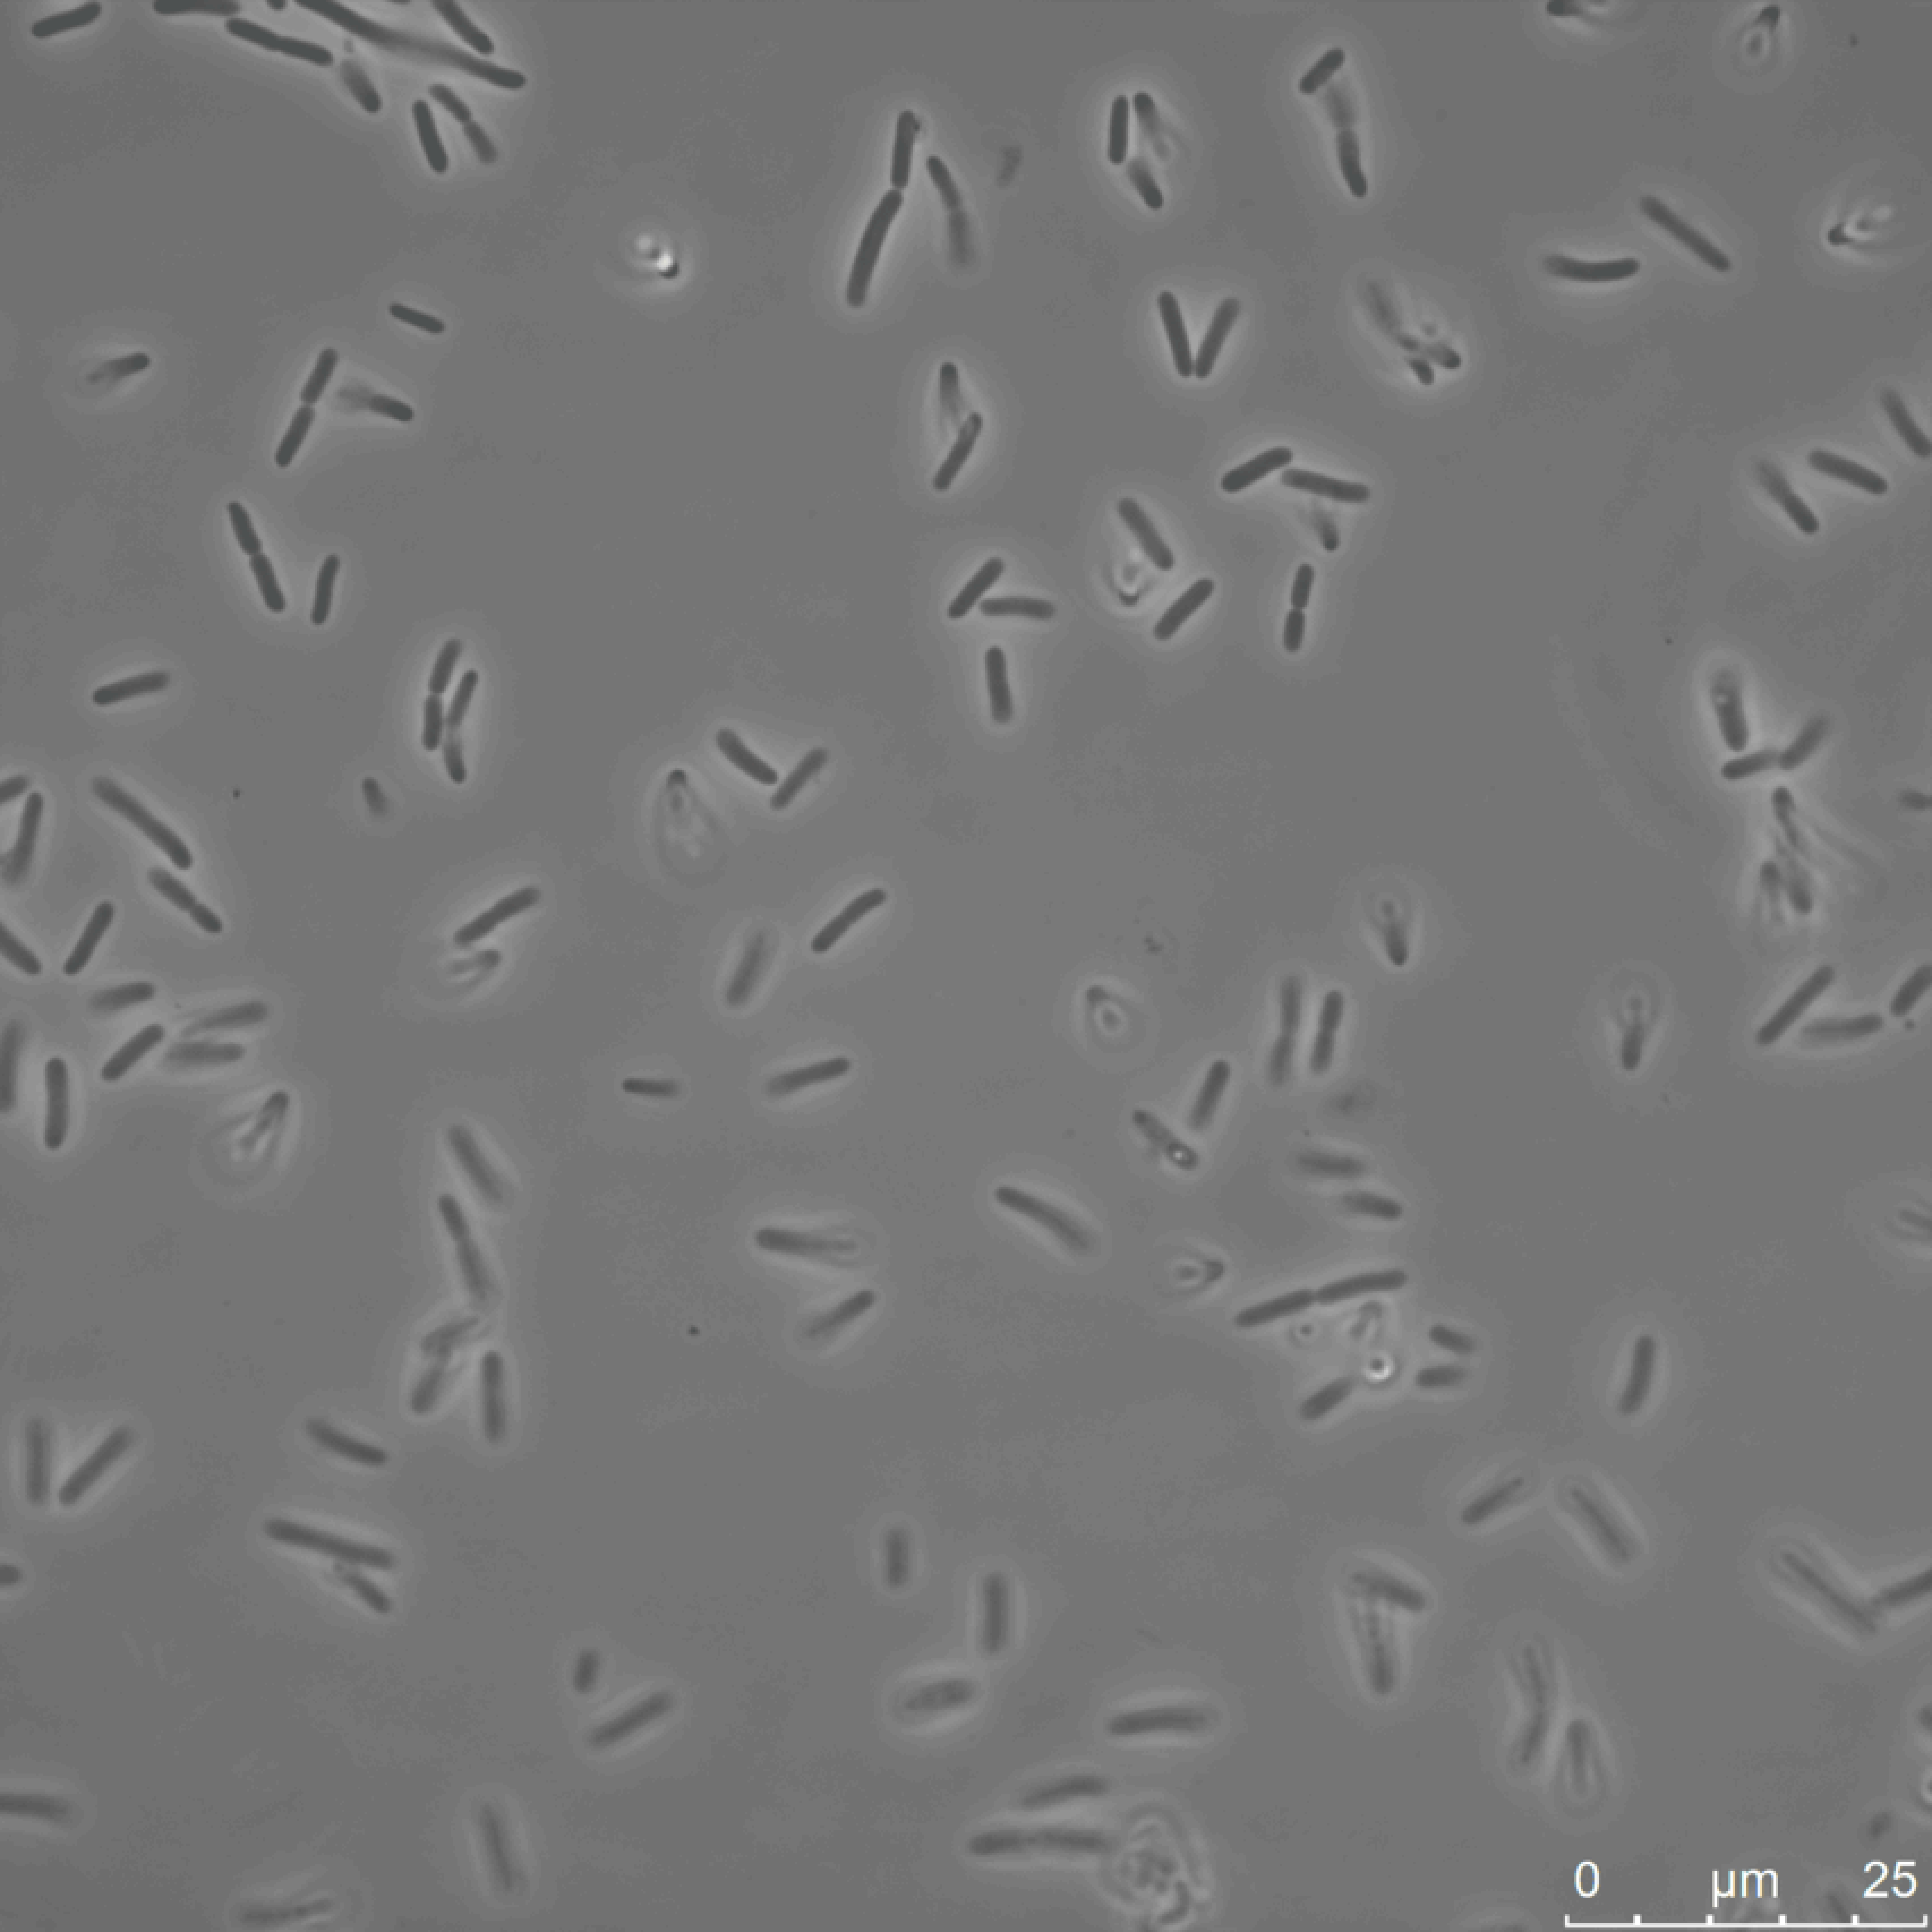
\includegraphics{TT01U1_1_NOGREEN-crunch-lighter-resample.pdf} &%
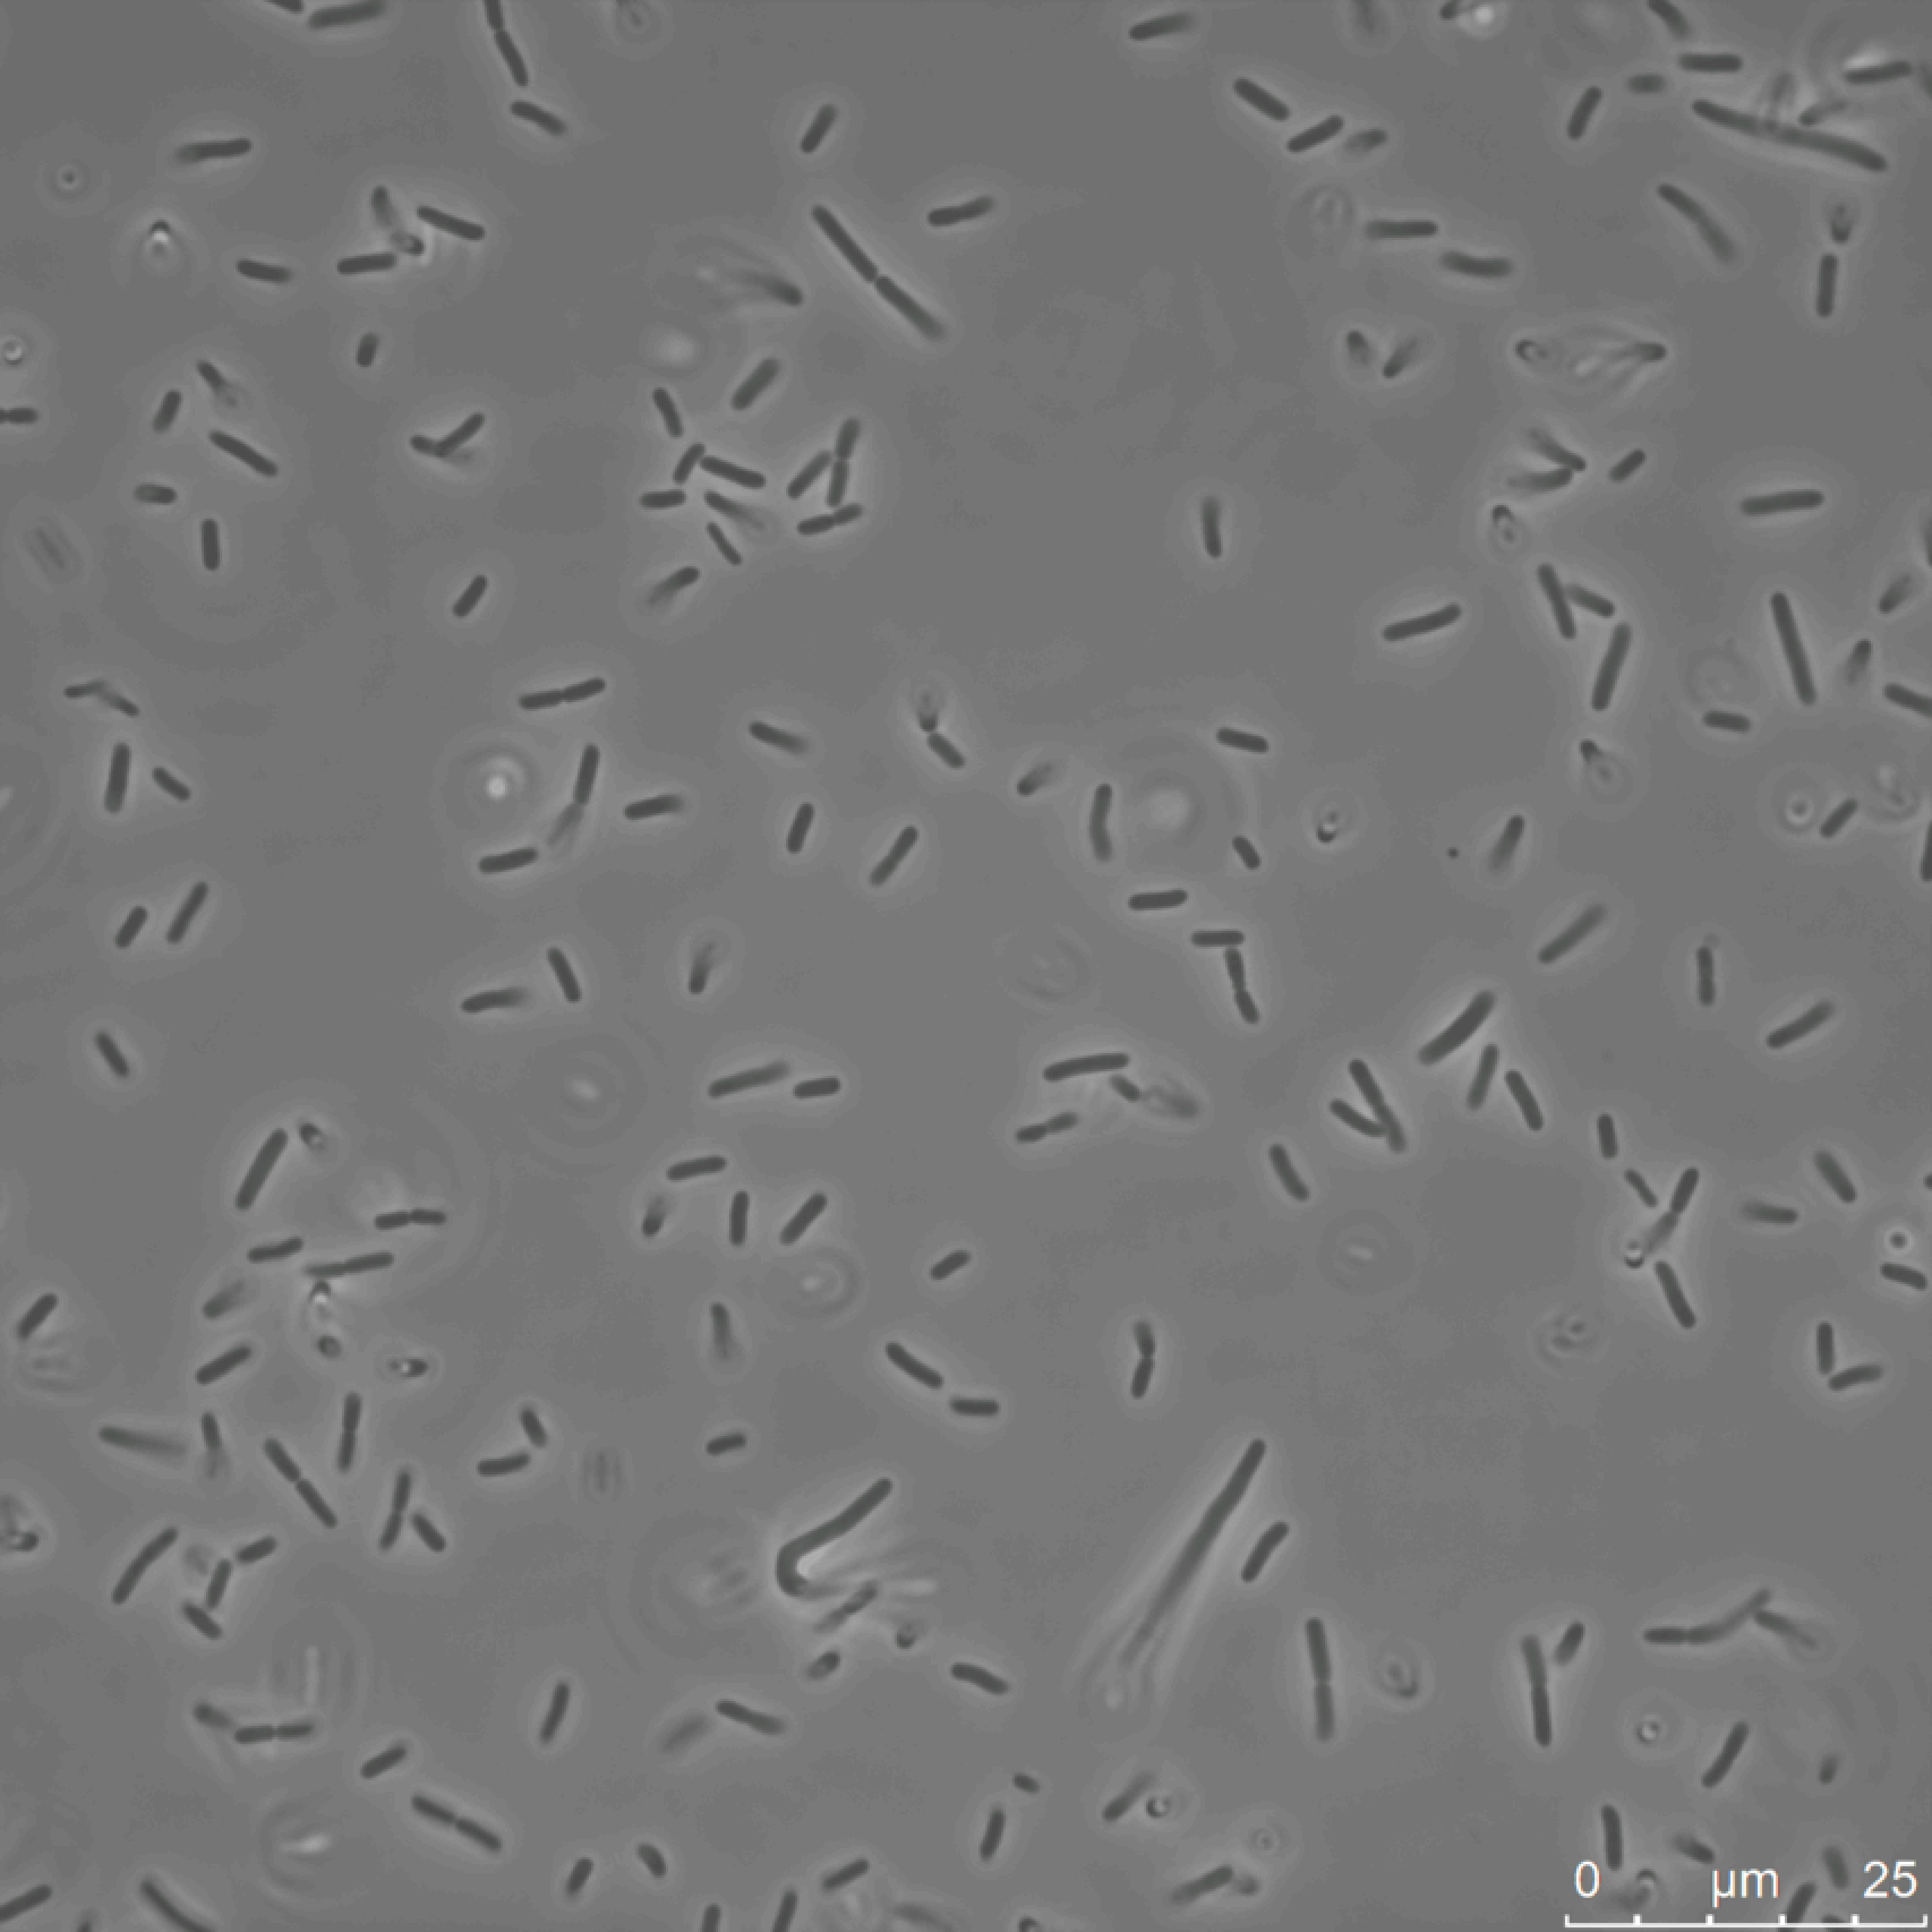
\includegraphics{TT01U1_5HR_5_LOWGREEN-crunch-lighter-resample.pdf} &%
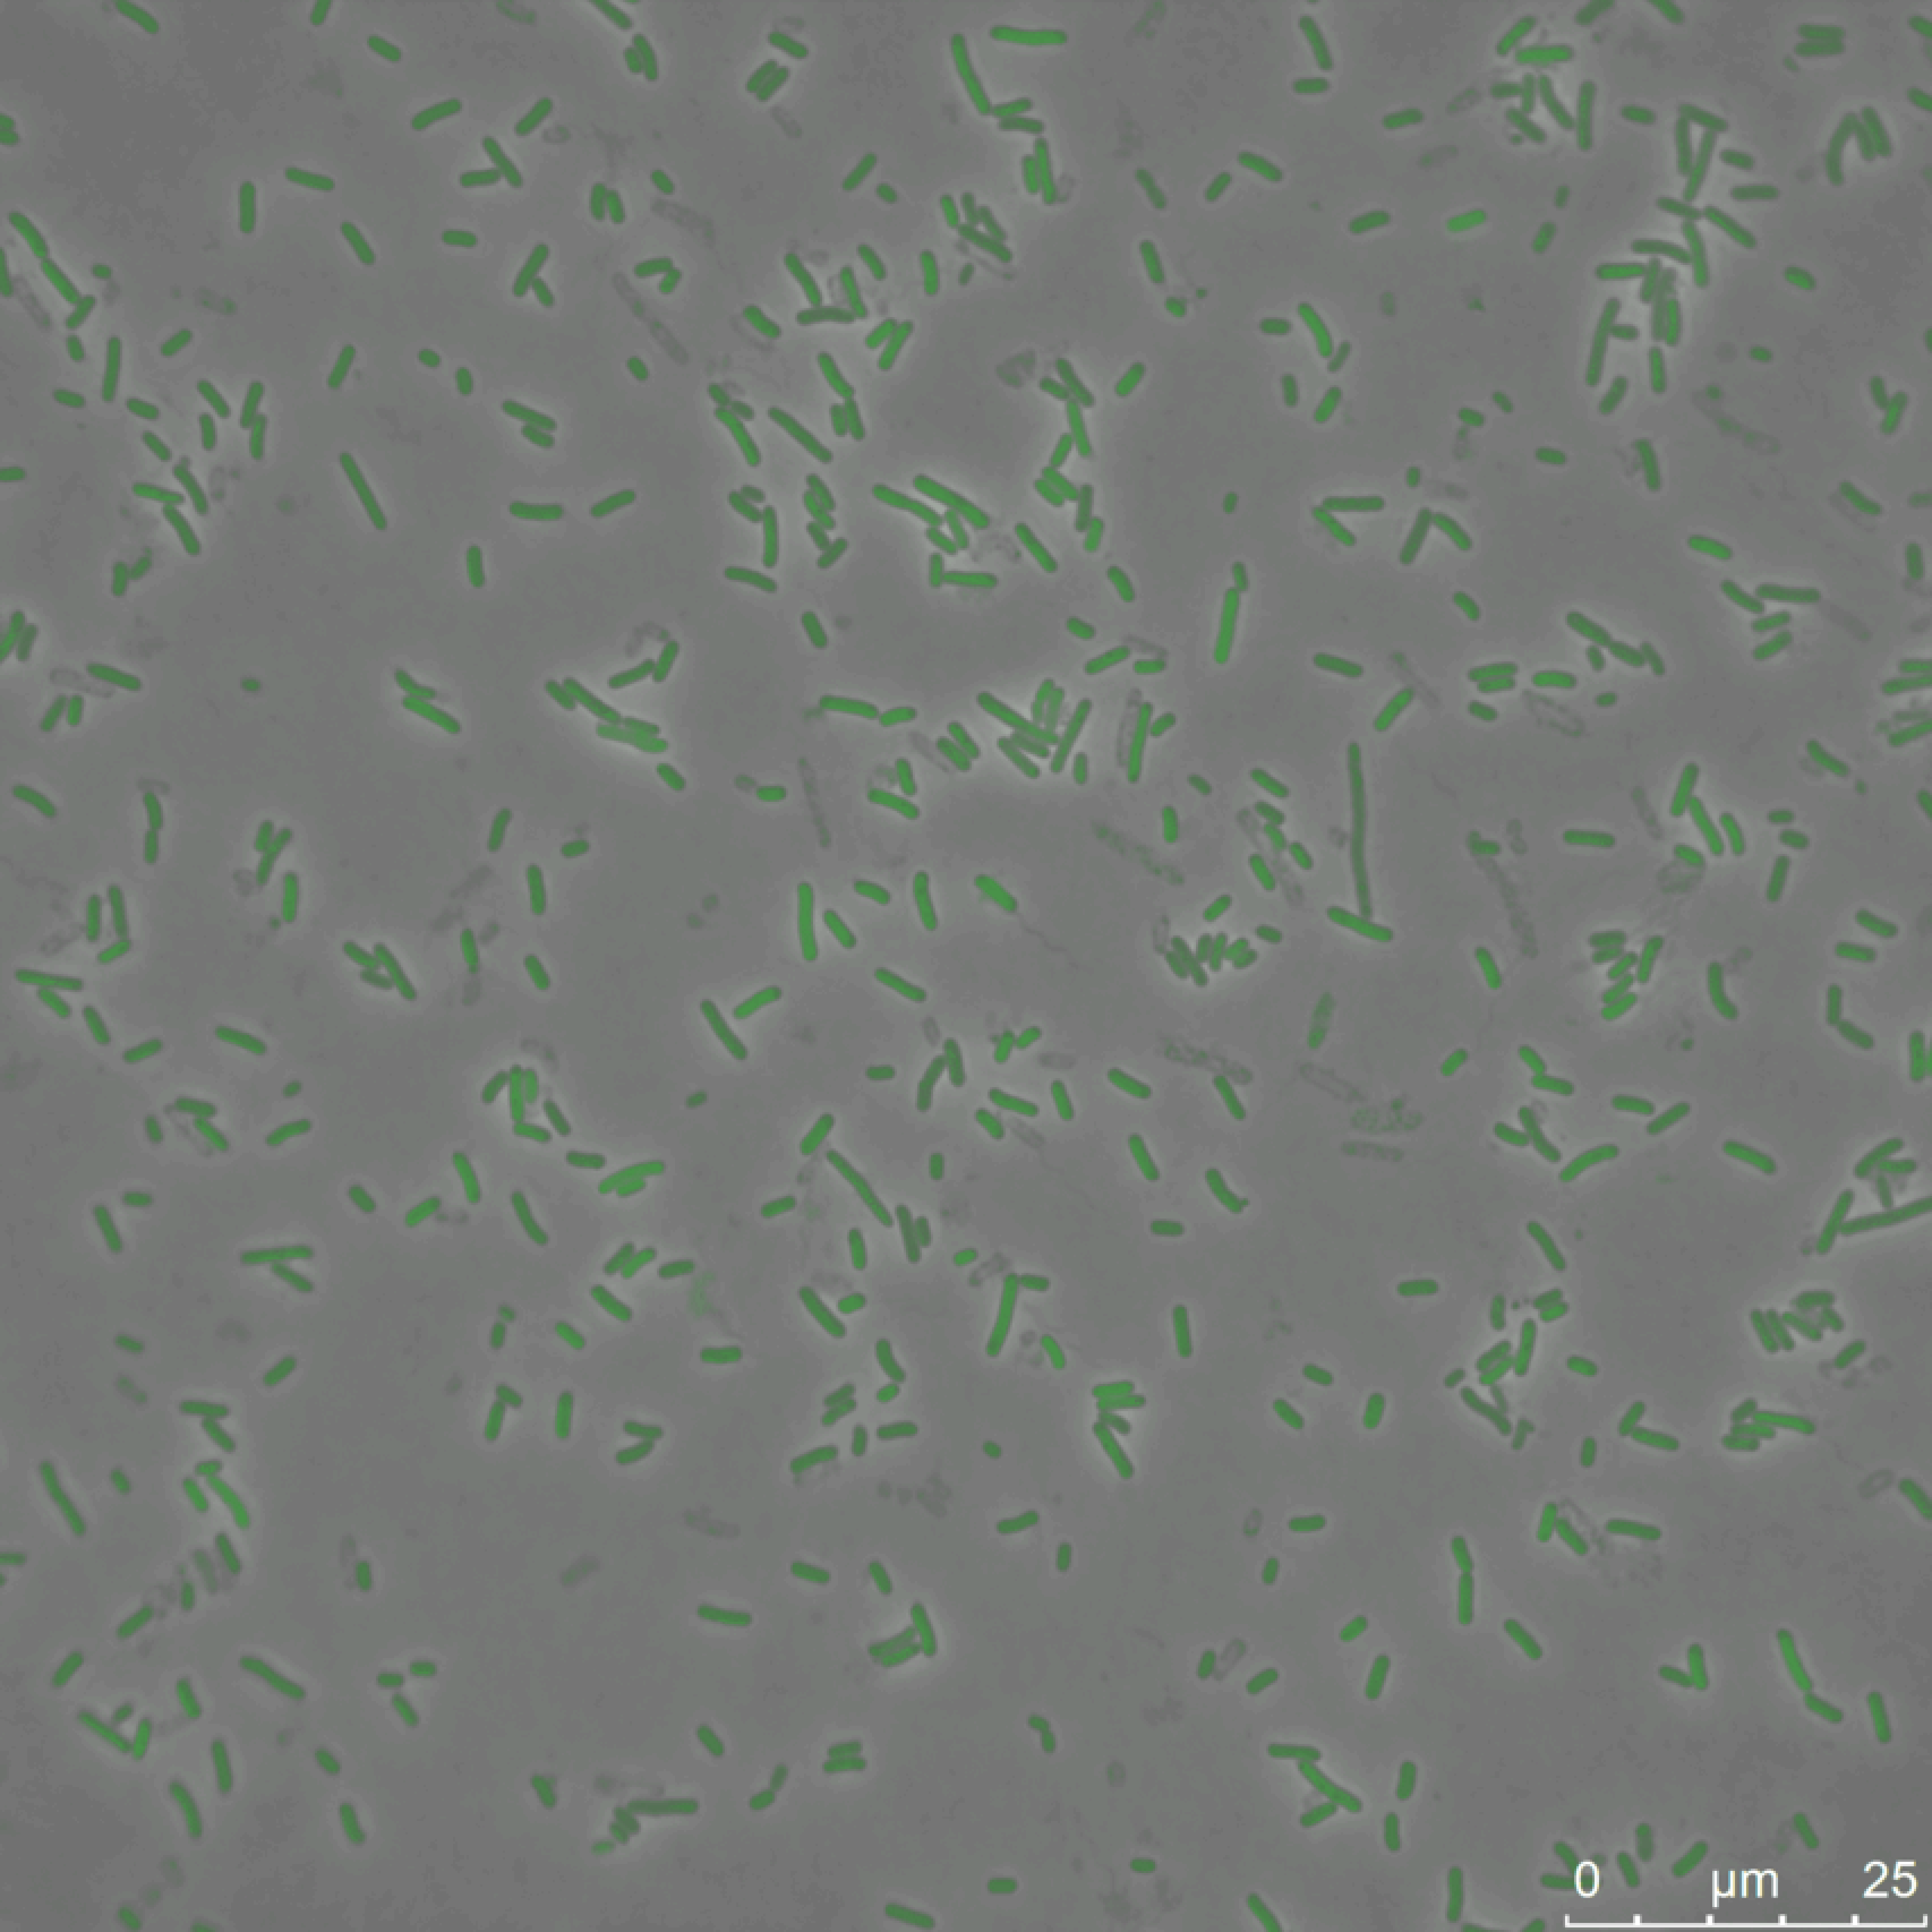
\includegraphics{TT01U1_24HR_1_GREEN-crunch-lighter-resample.pdf} &%
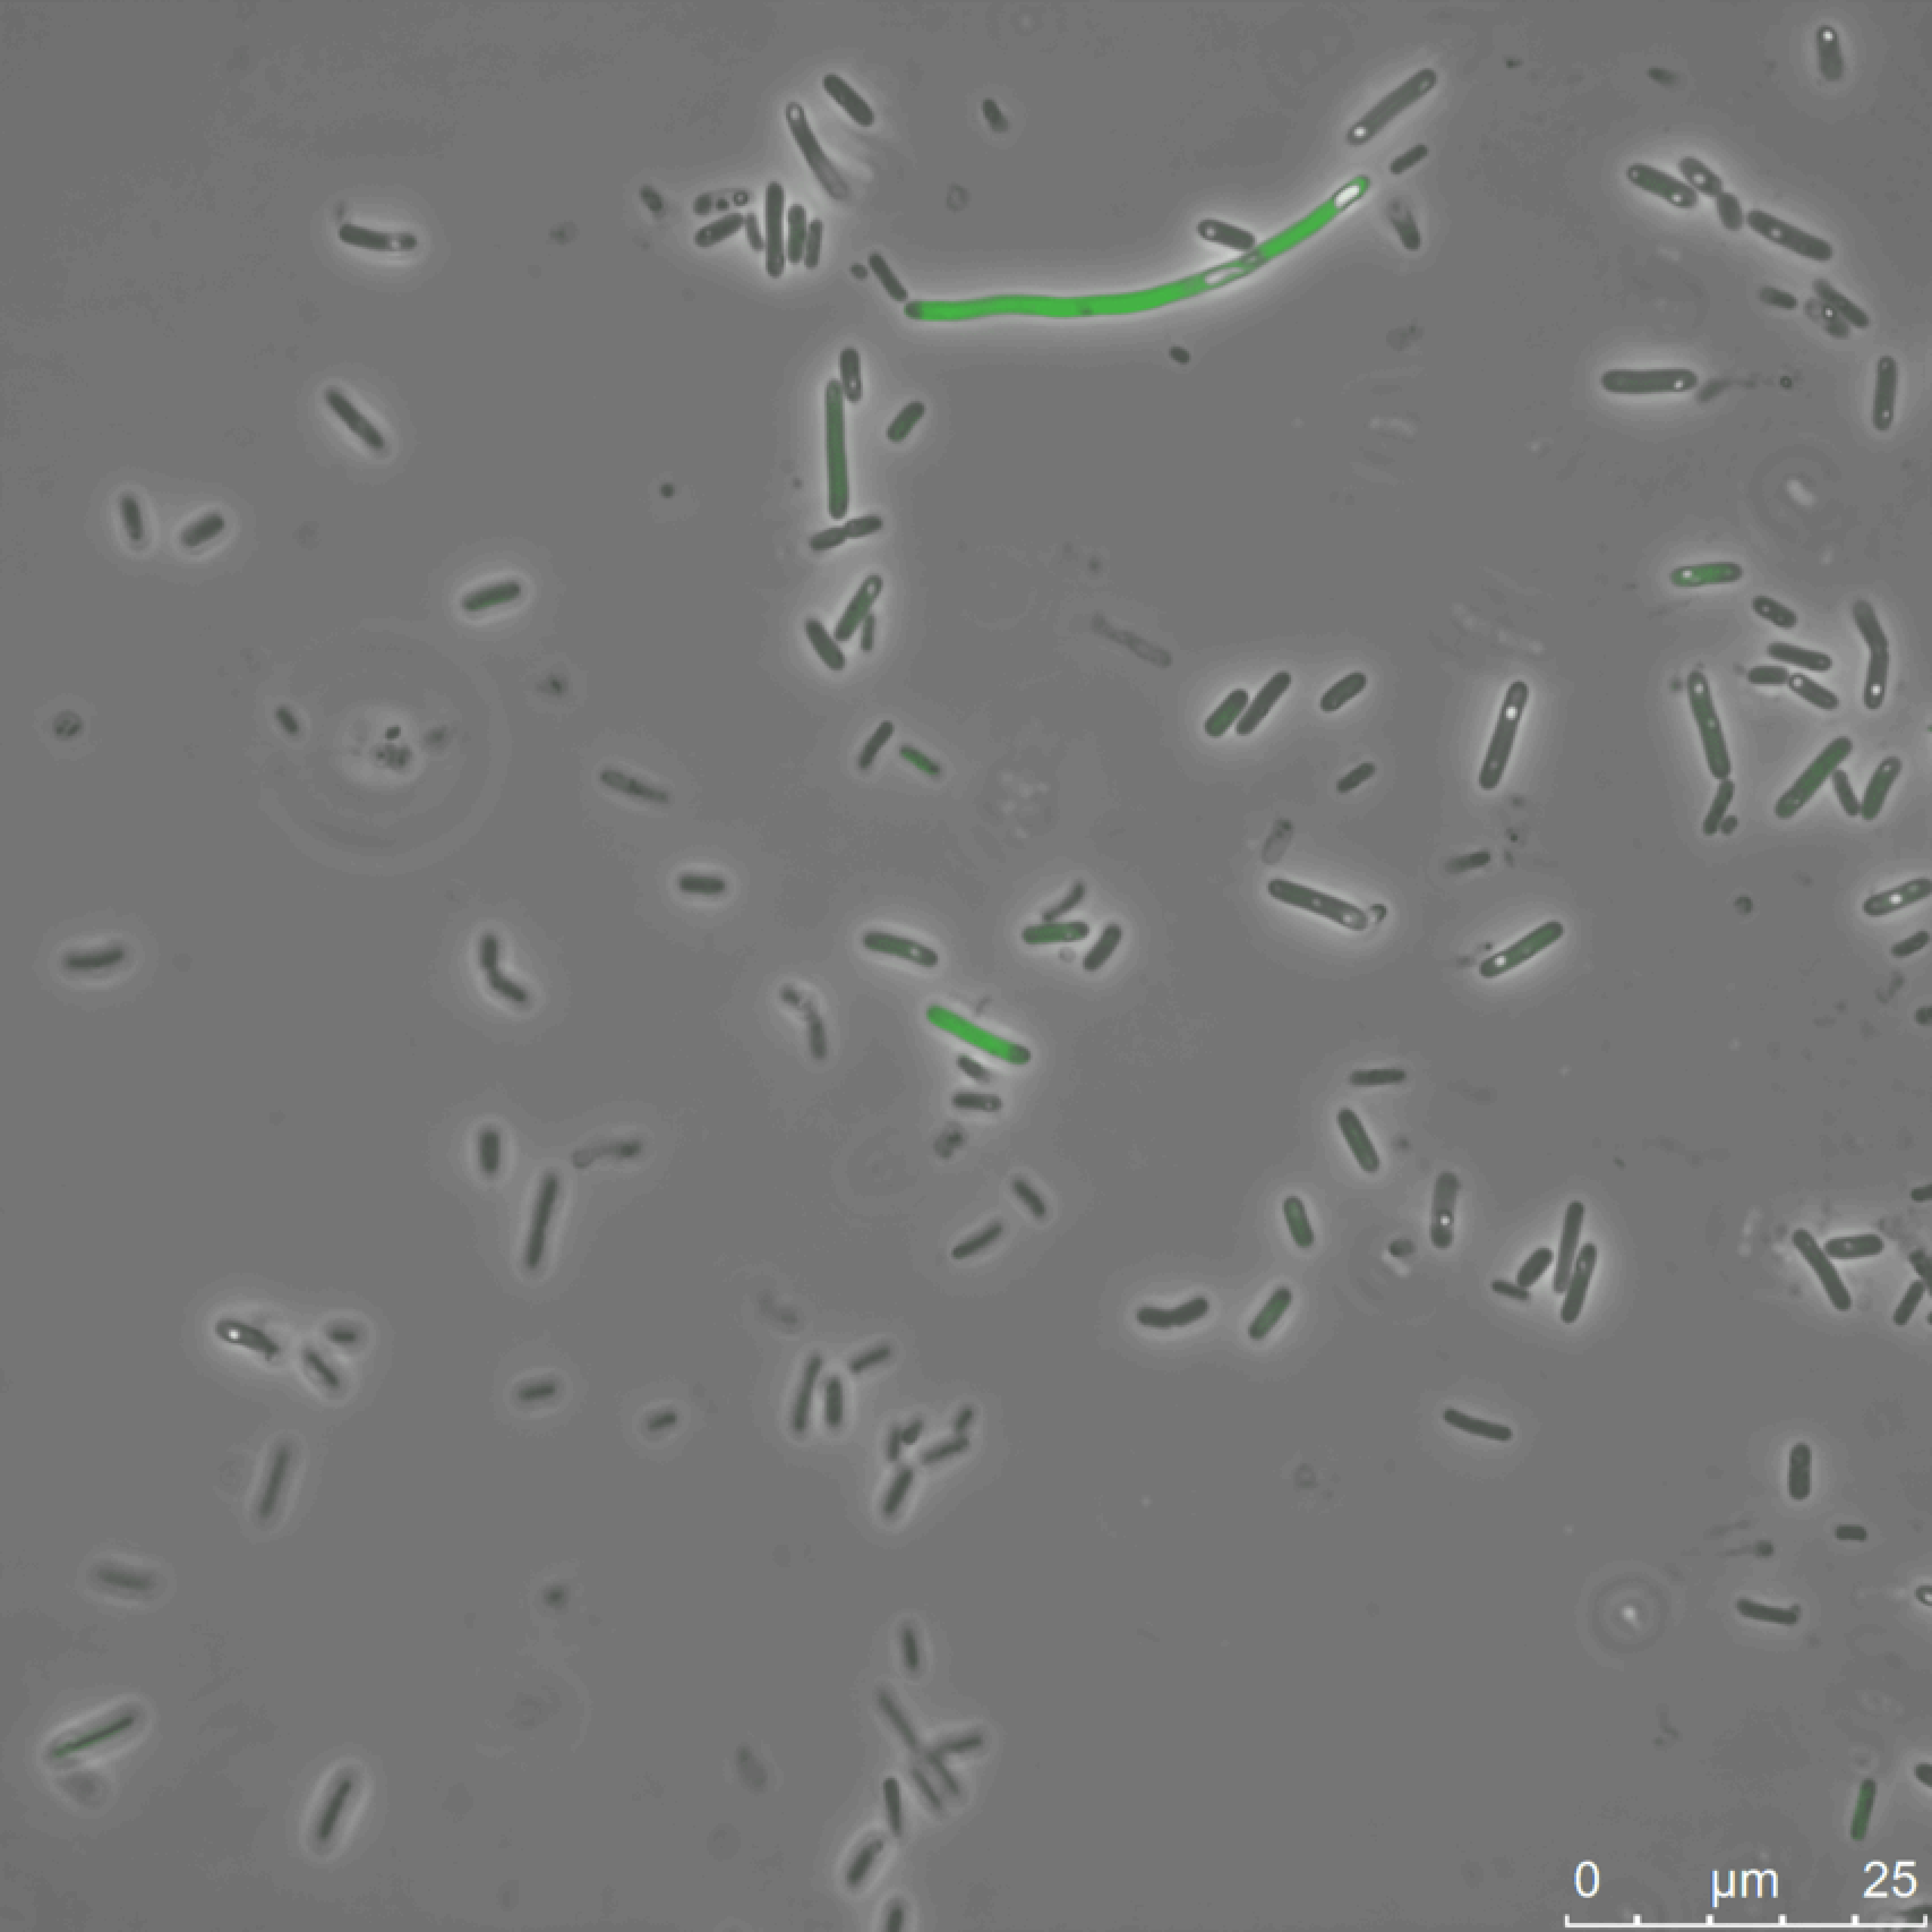
\includegraphics{TT01U1_72HR_1_GREEN-crunch-lighter-resample.pdf} \\[-0.5ex]

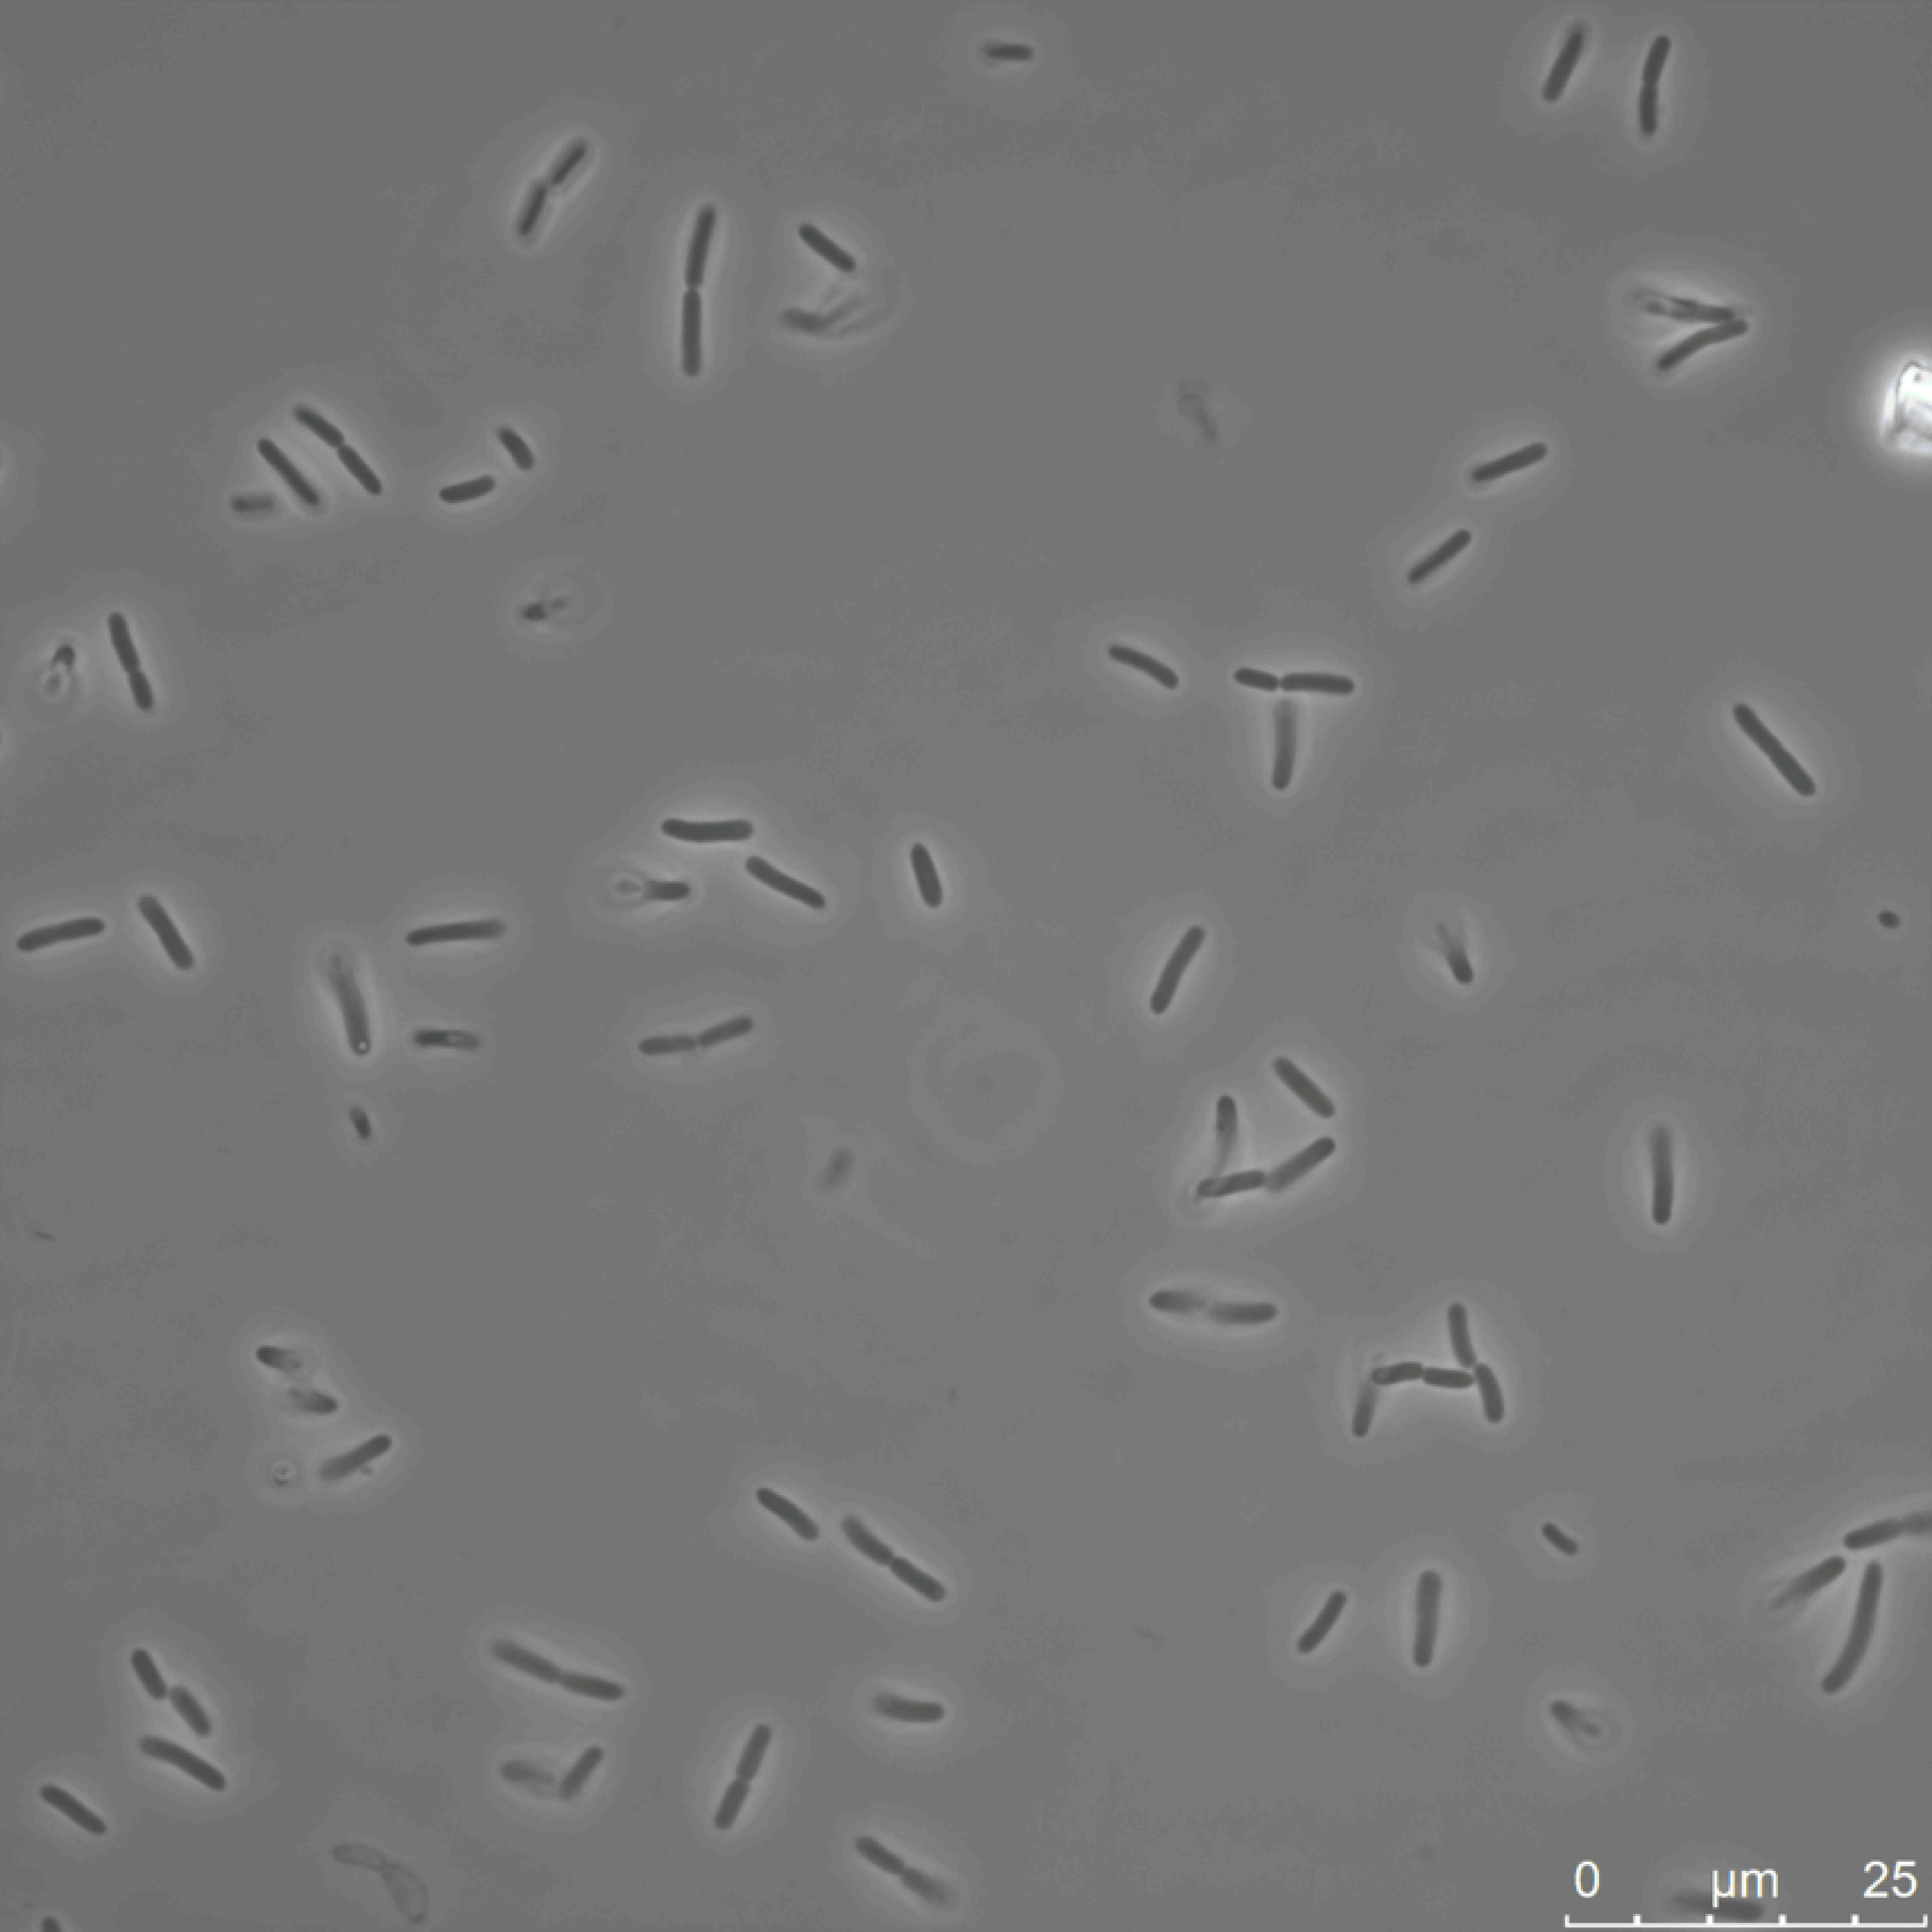
\includegraphics{TT01U1_2_NOGREEN-crunch-lighter-resample.pdf} &%
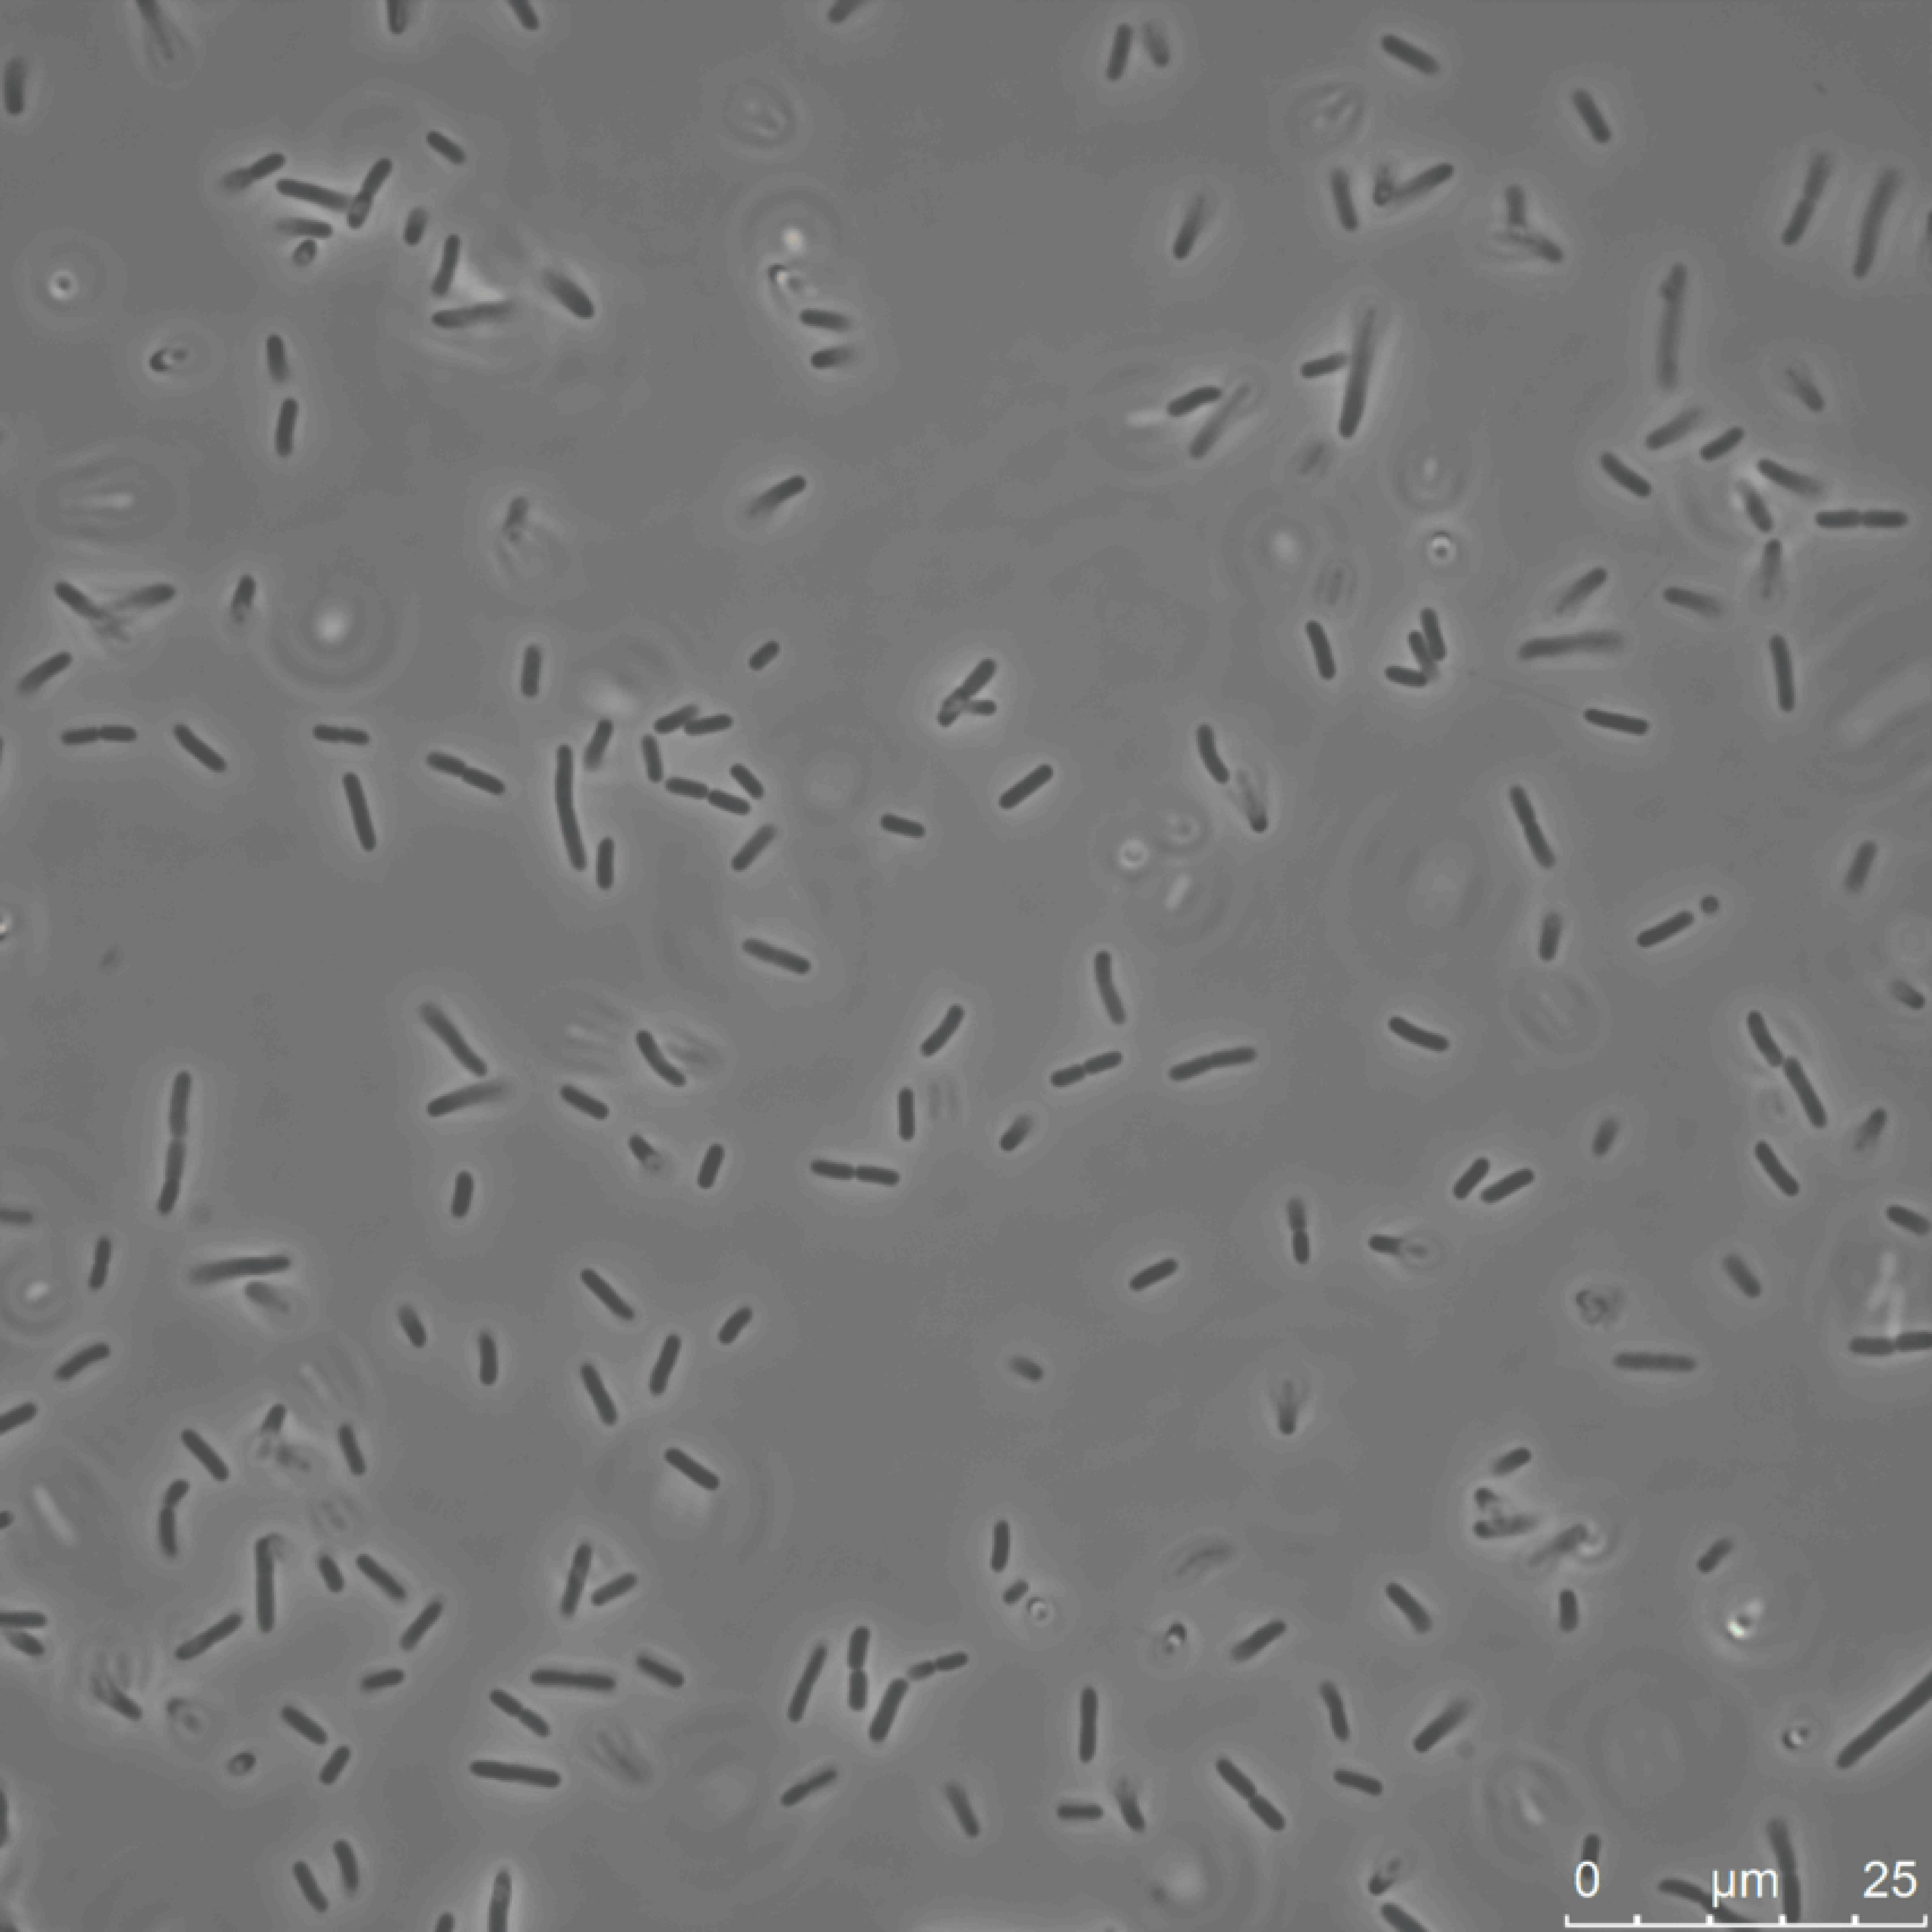
\includegraphics{TT01U1_5HR_2_NOGREEN-crunch-lighter-resample.pdf} &%
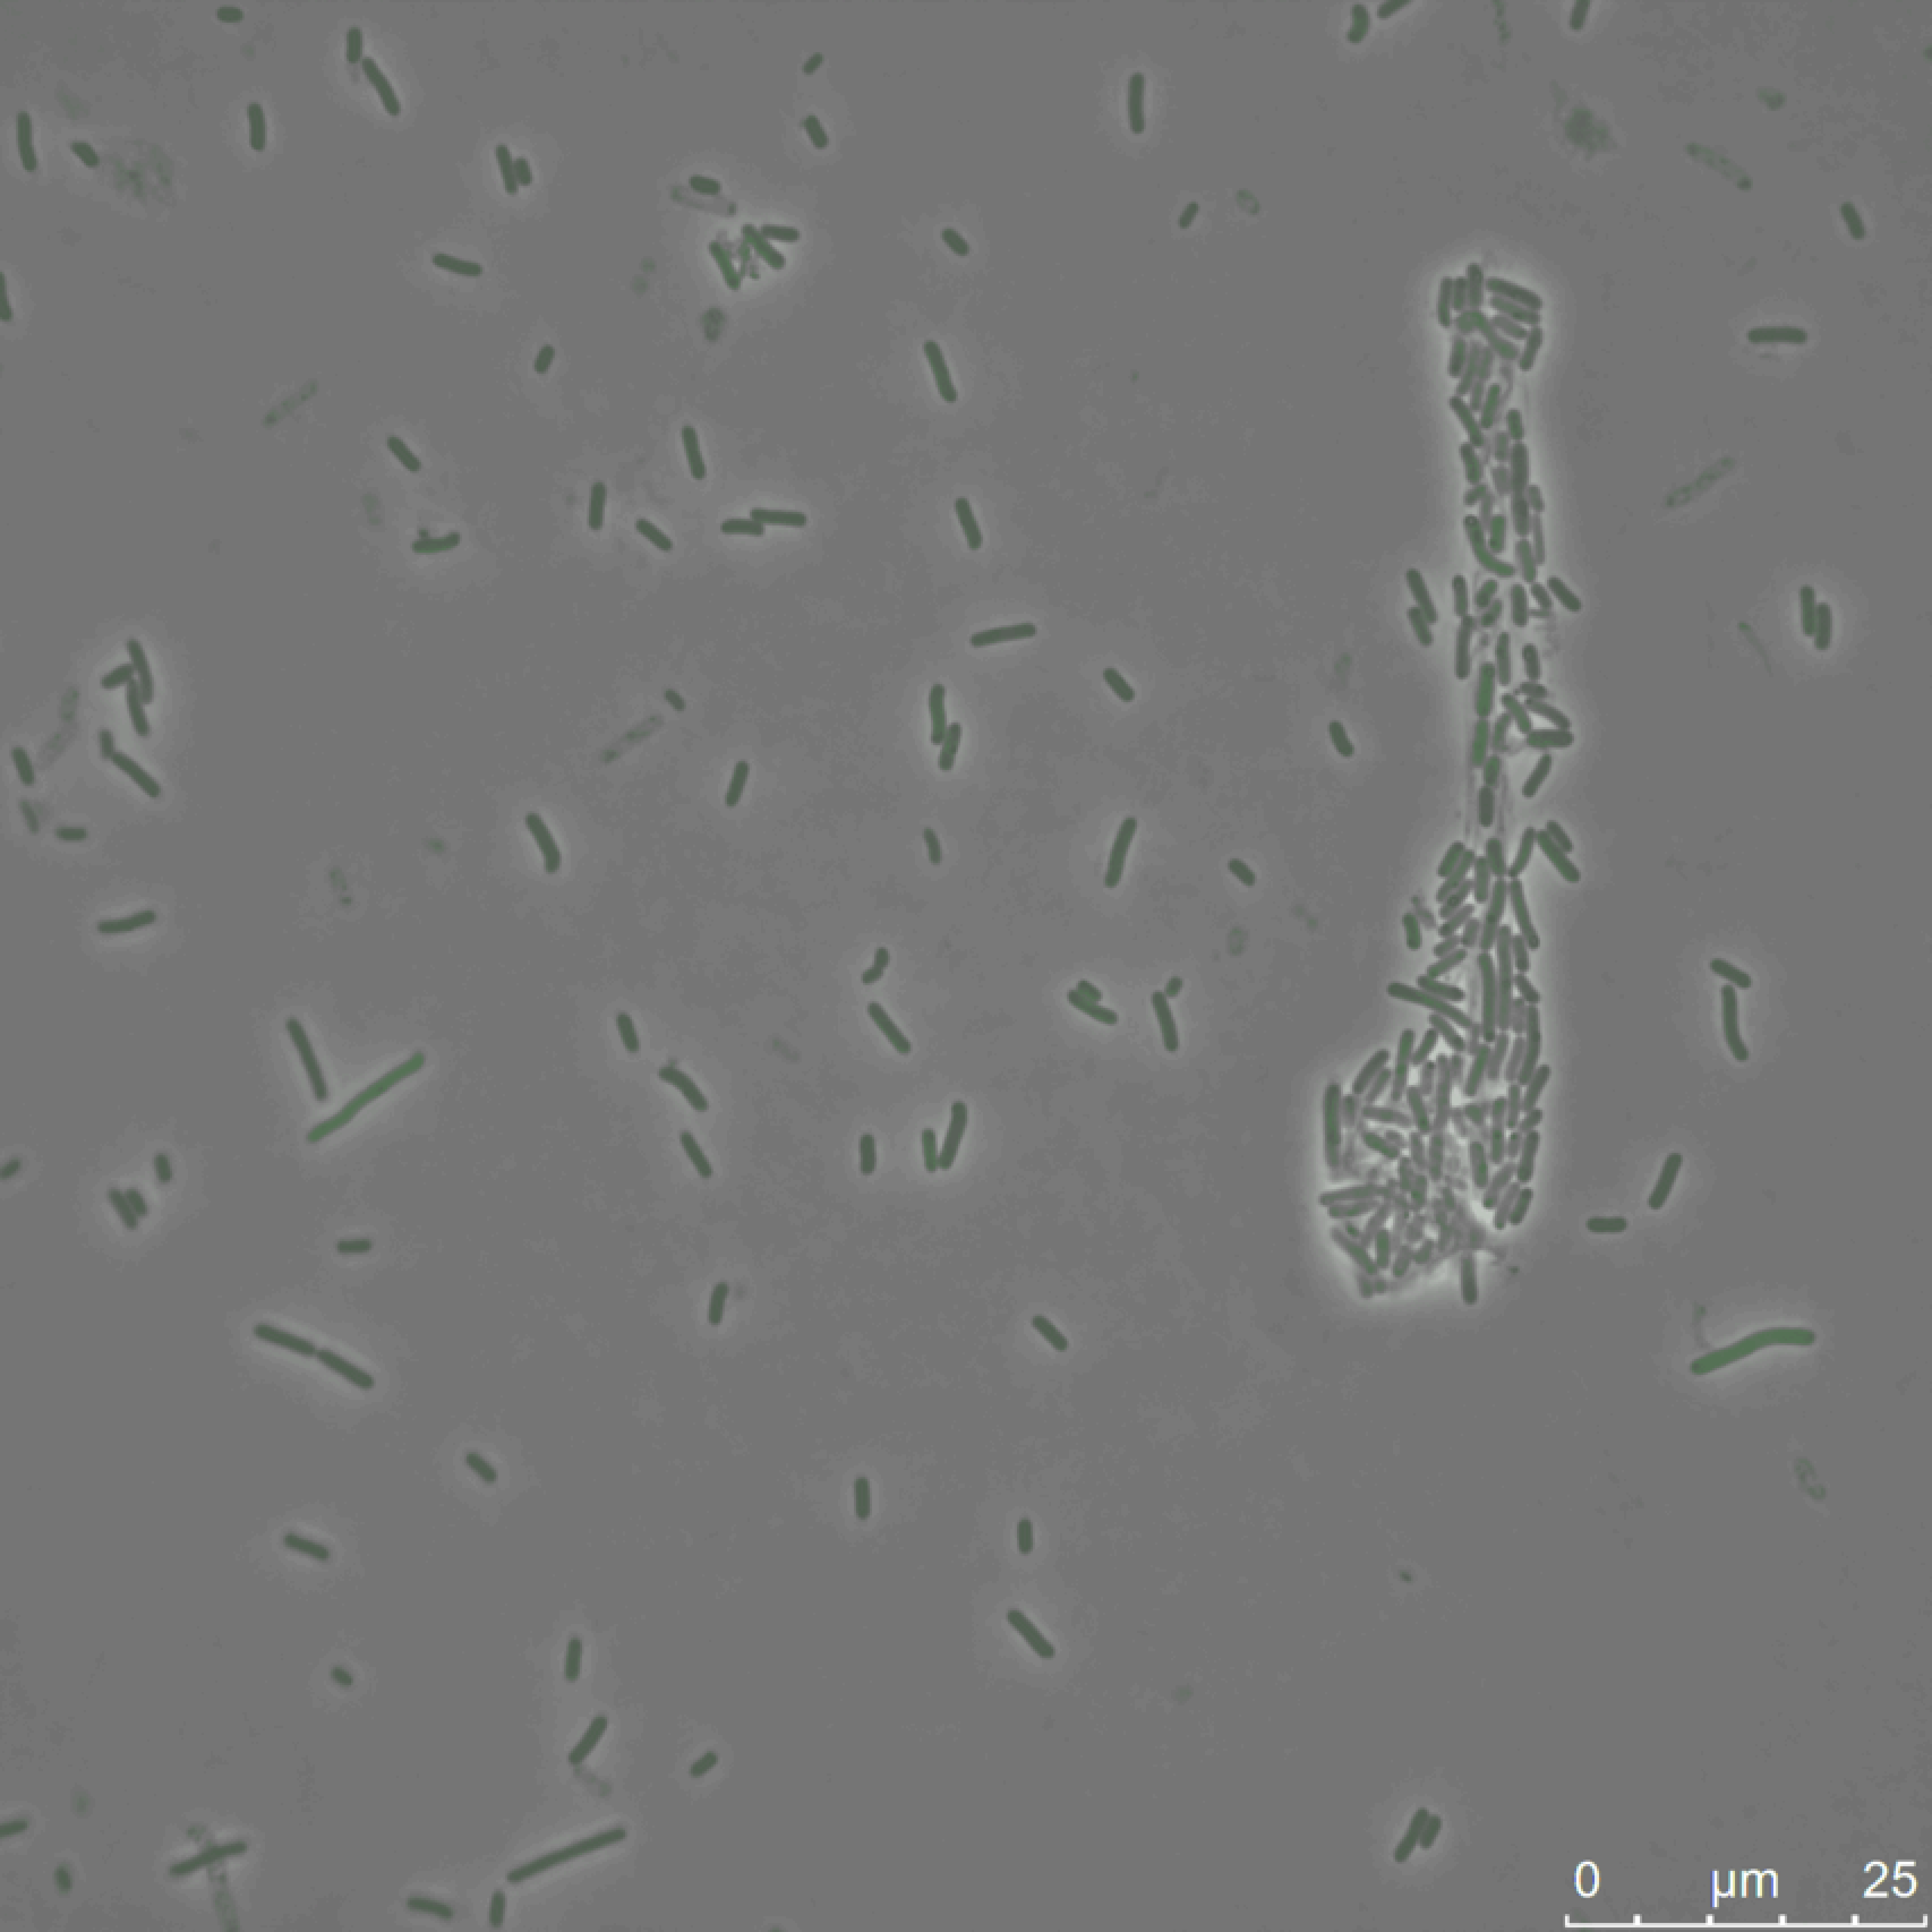
\includegraphics{TT01U1_24HR_2_LOWGREEN-crunch-lighter-resample.pdf} &%
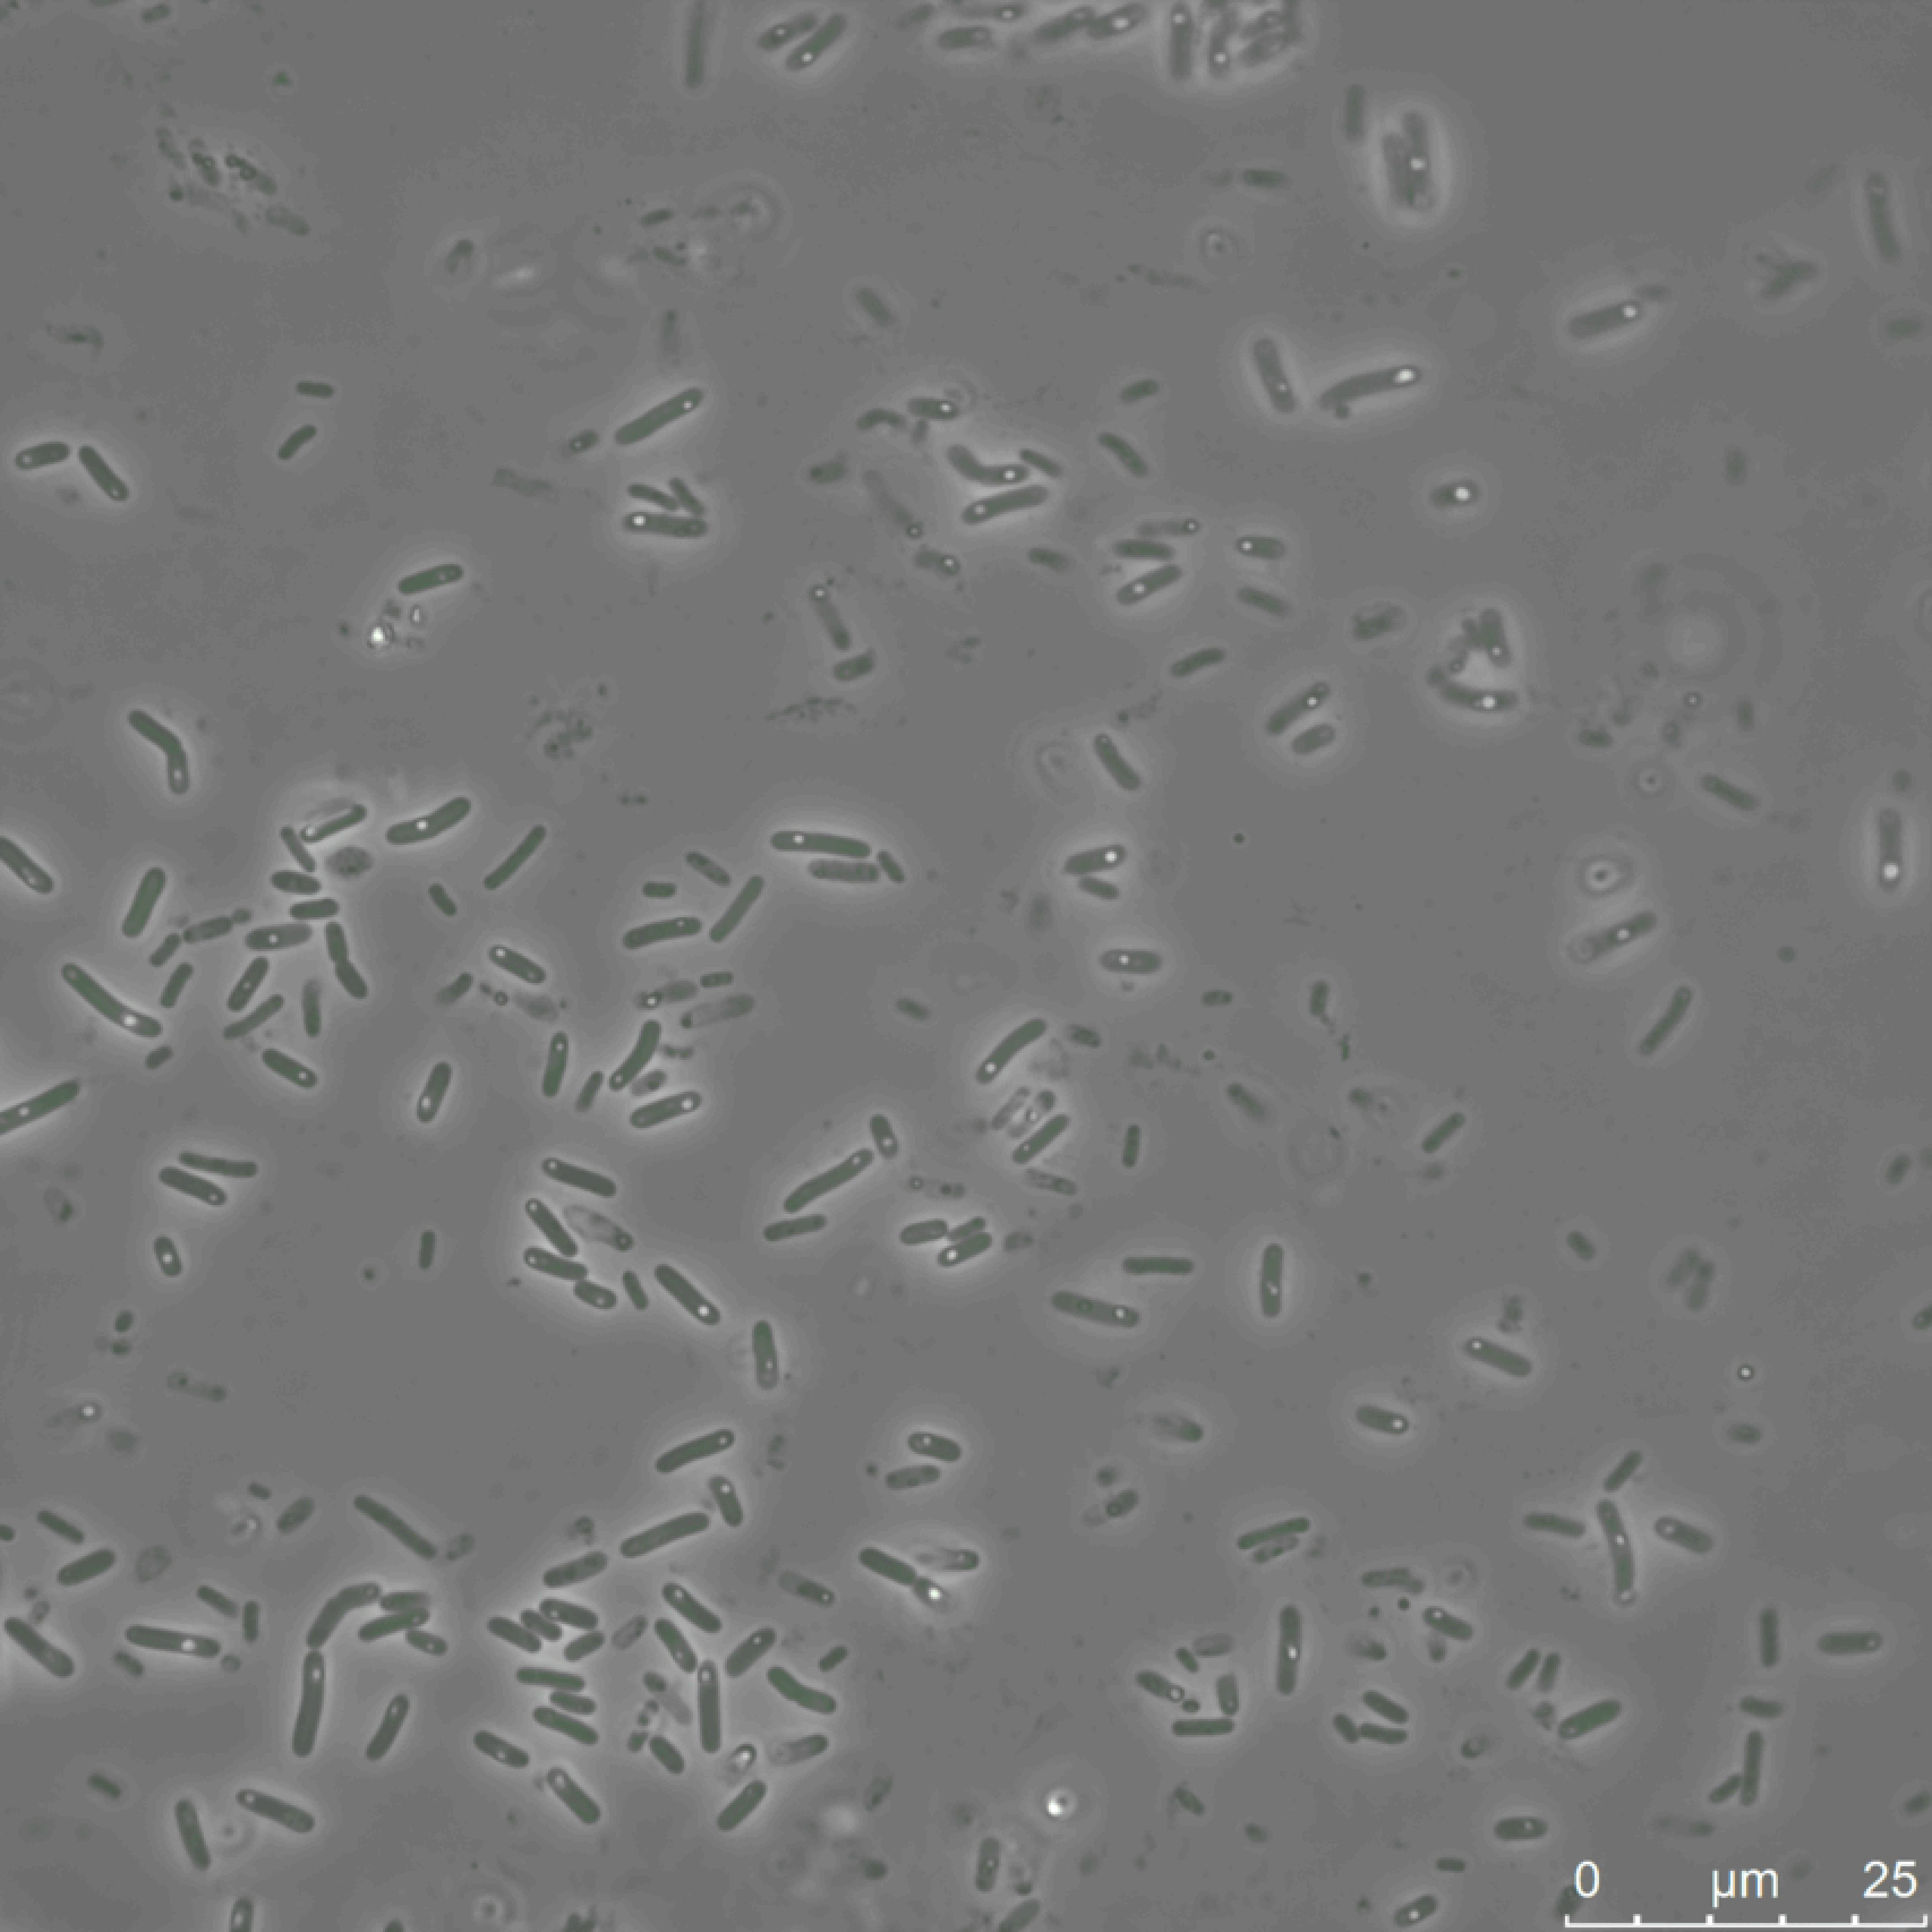
\includegraphics{TT01U1_72HR_2_LOWGREEN-crunch-lighter-resample.pdf} \\[-0.5ex]

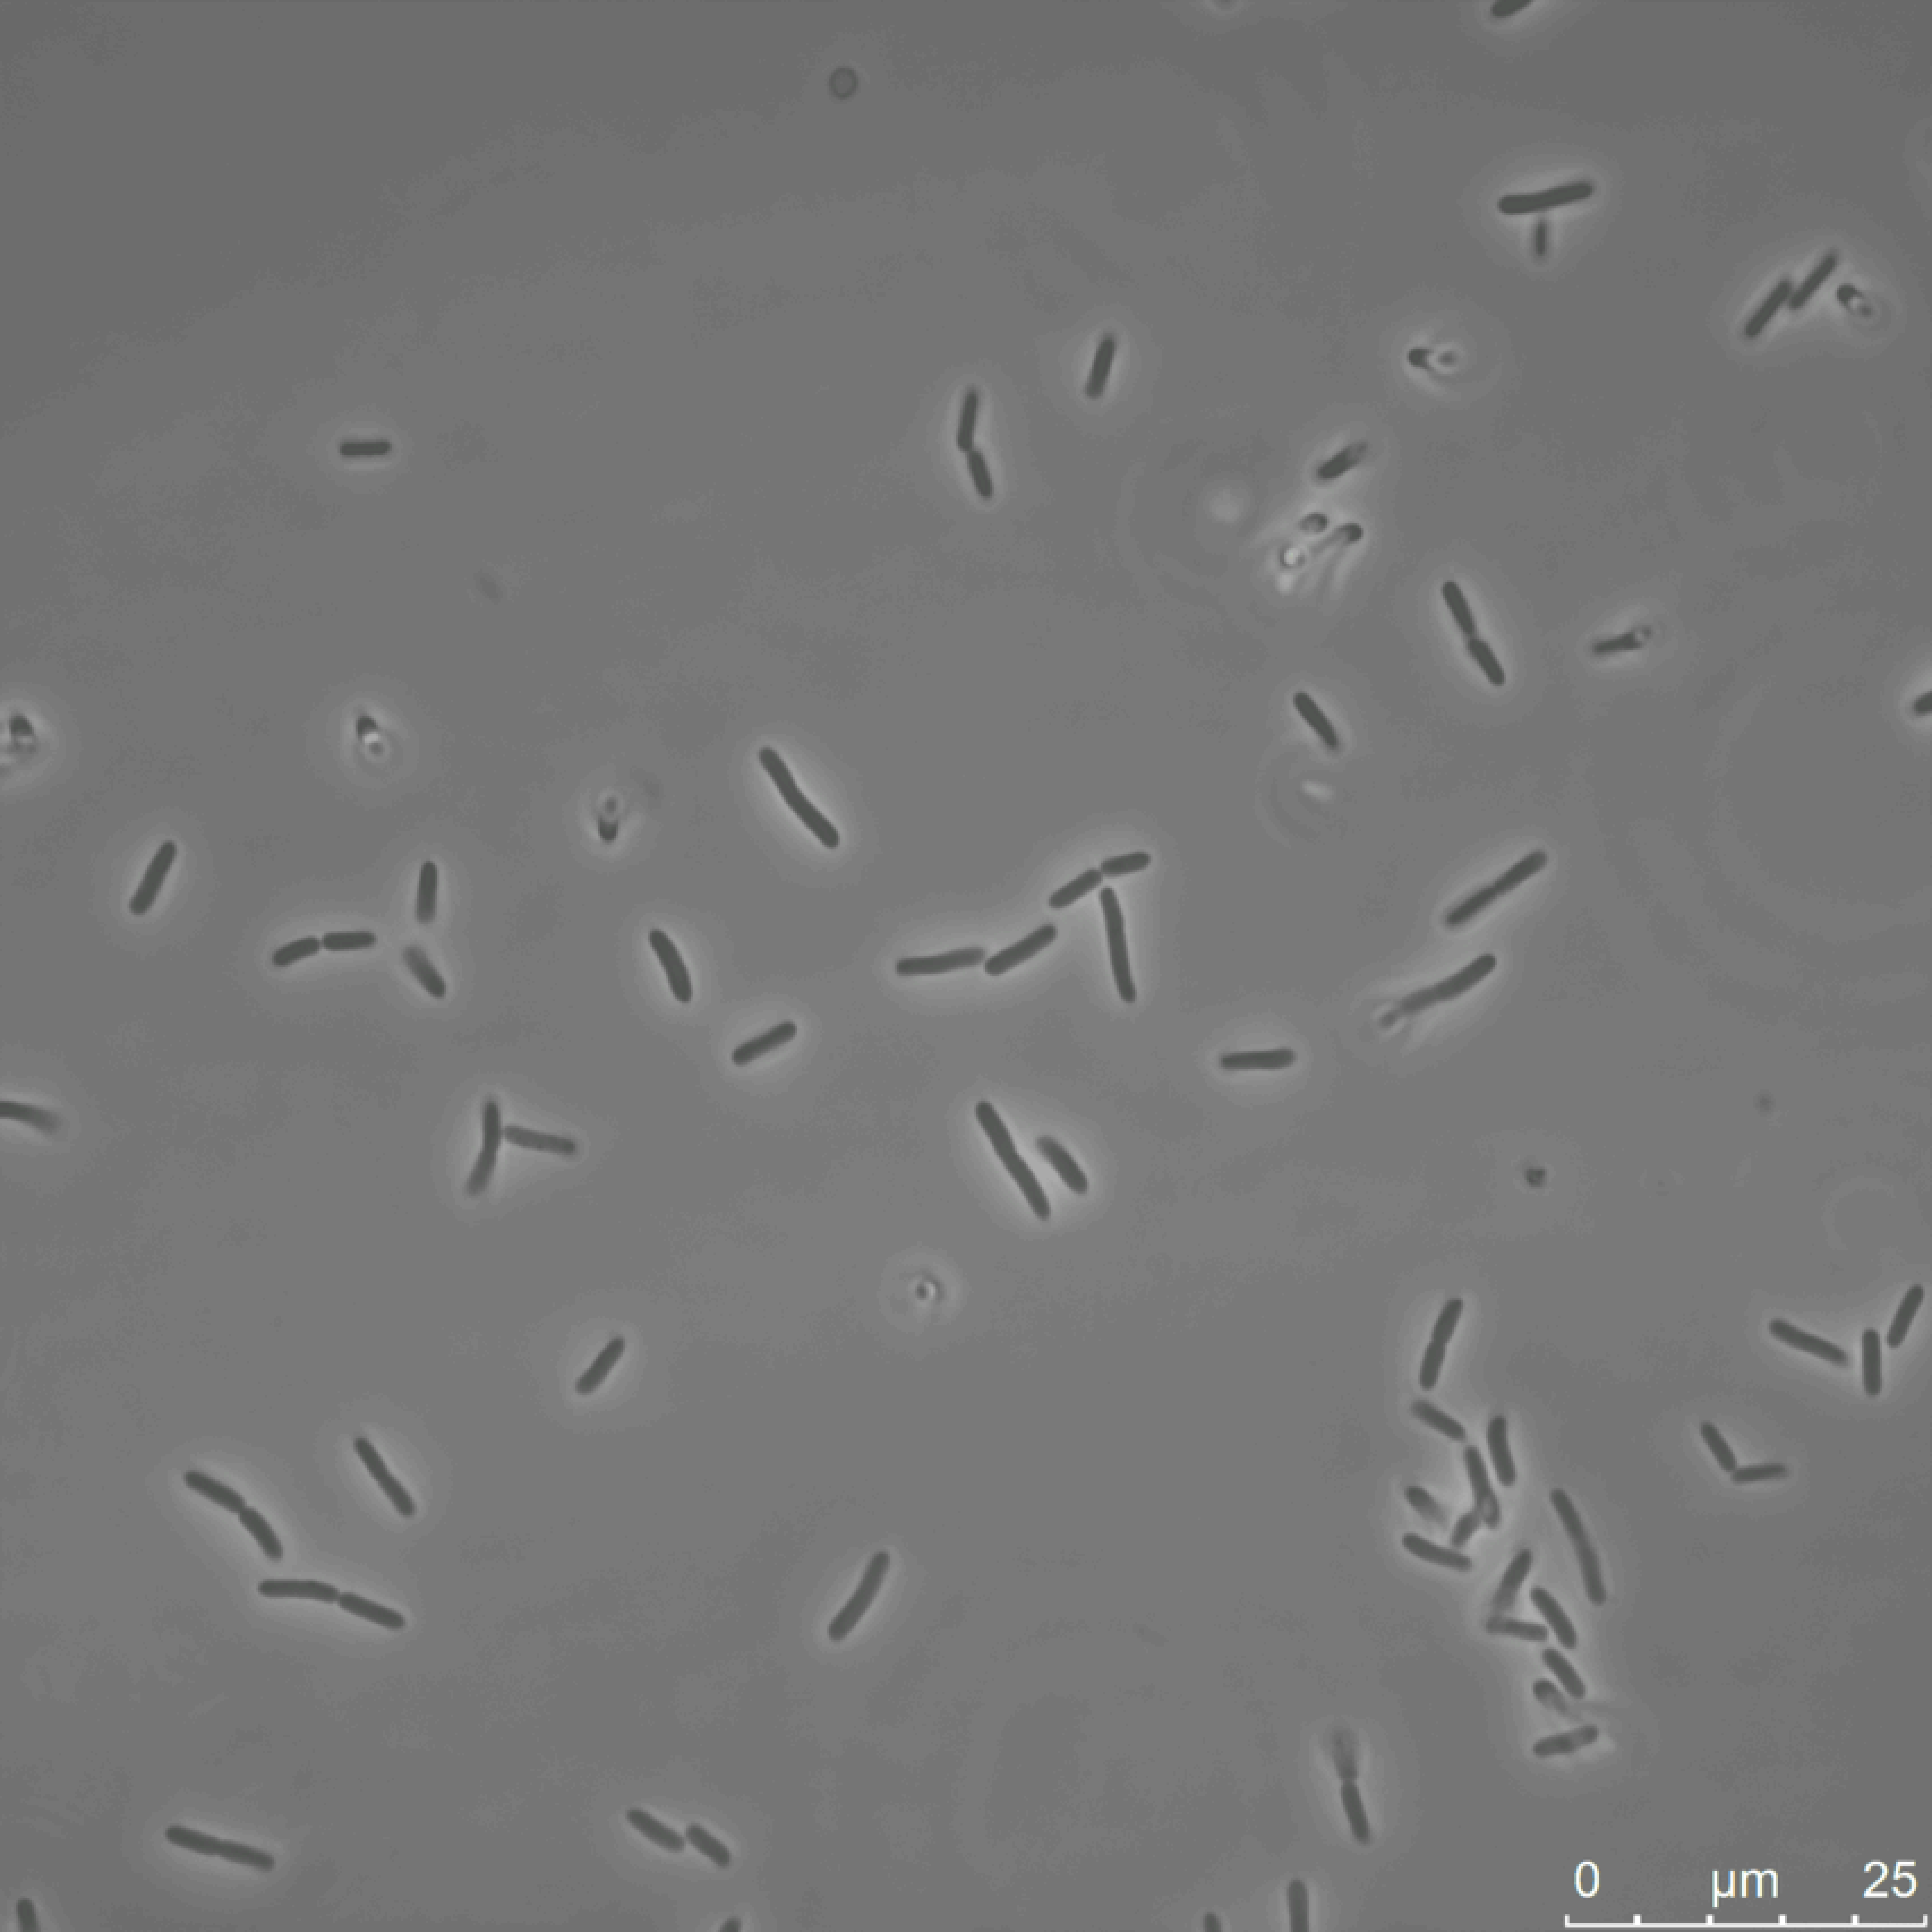
\includegraphics{TT01U1_3_NOGREEN-crunch-lighter-resample.pdf} &%
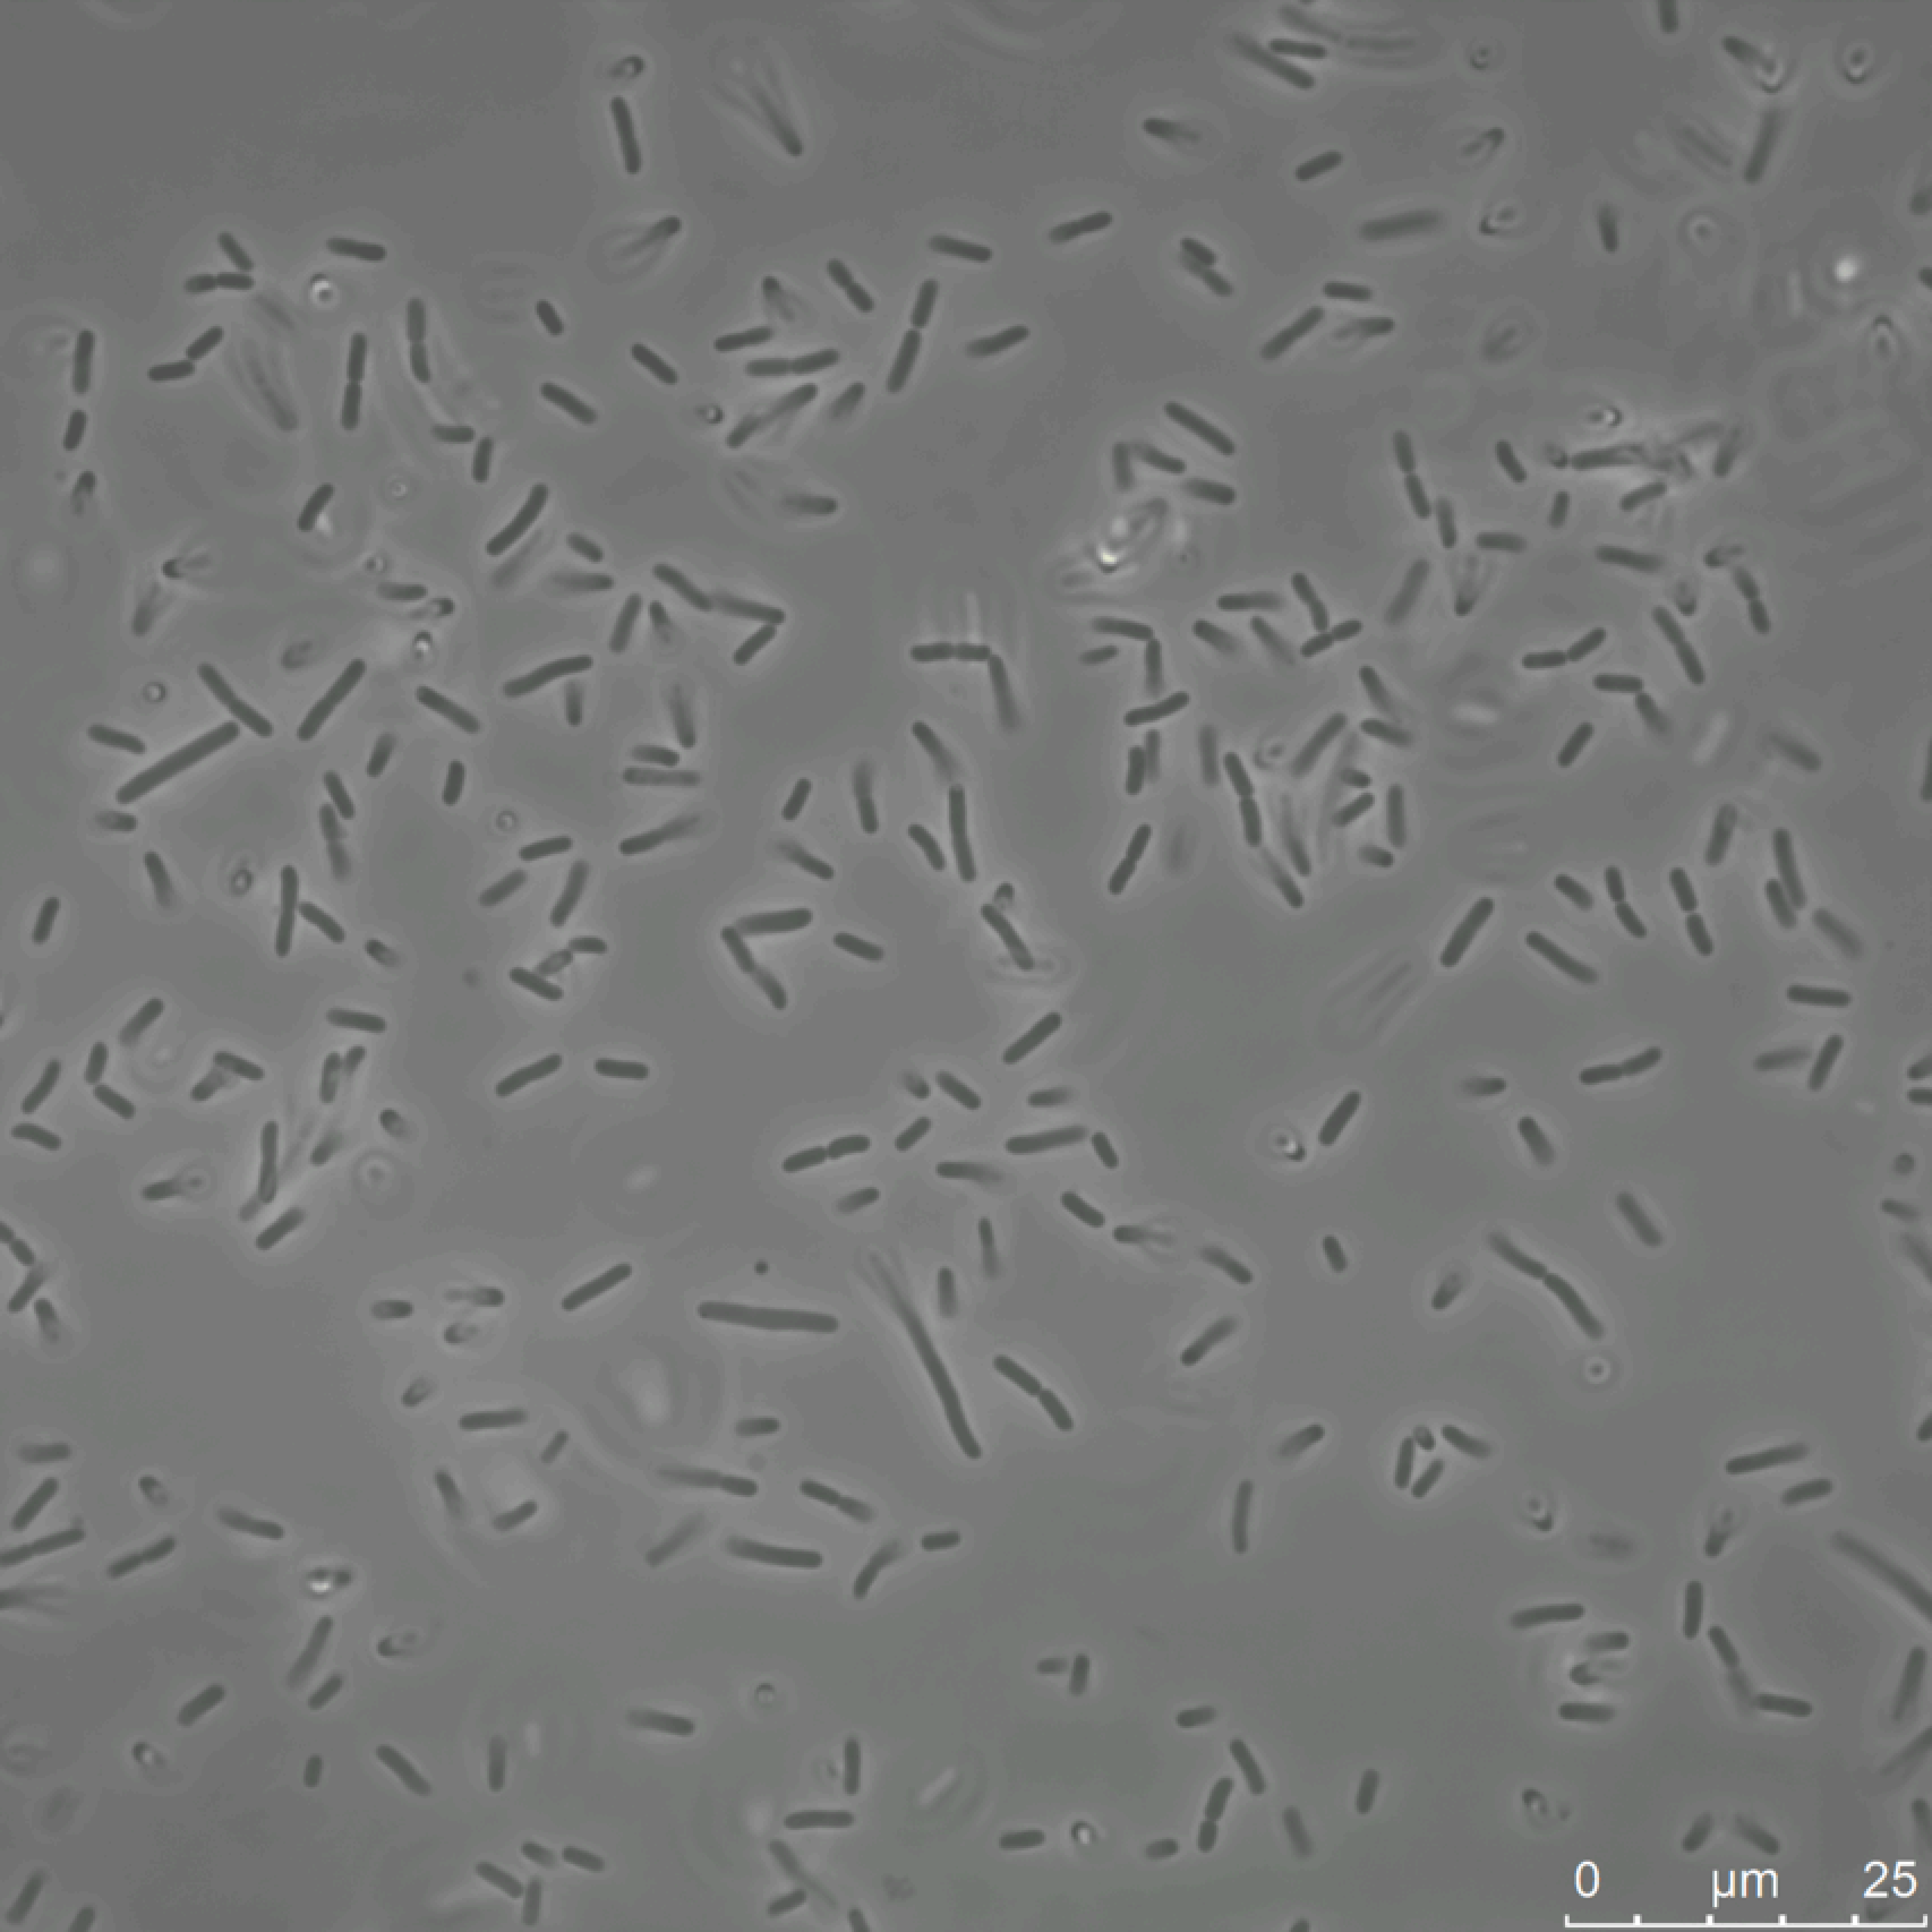
\includegraphics{TT01U1_5HR_3_LOWGREEN-crunch-lighter-resample.pdf} &%
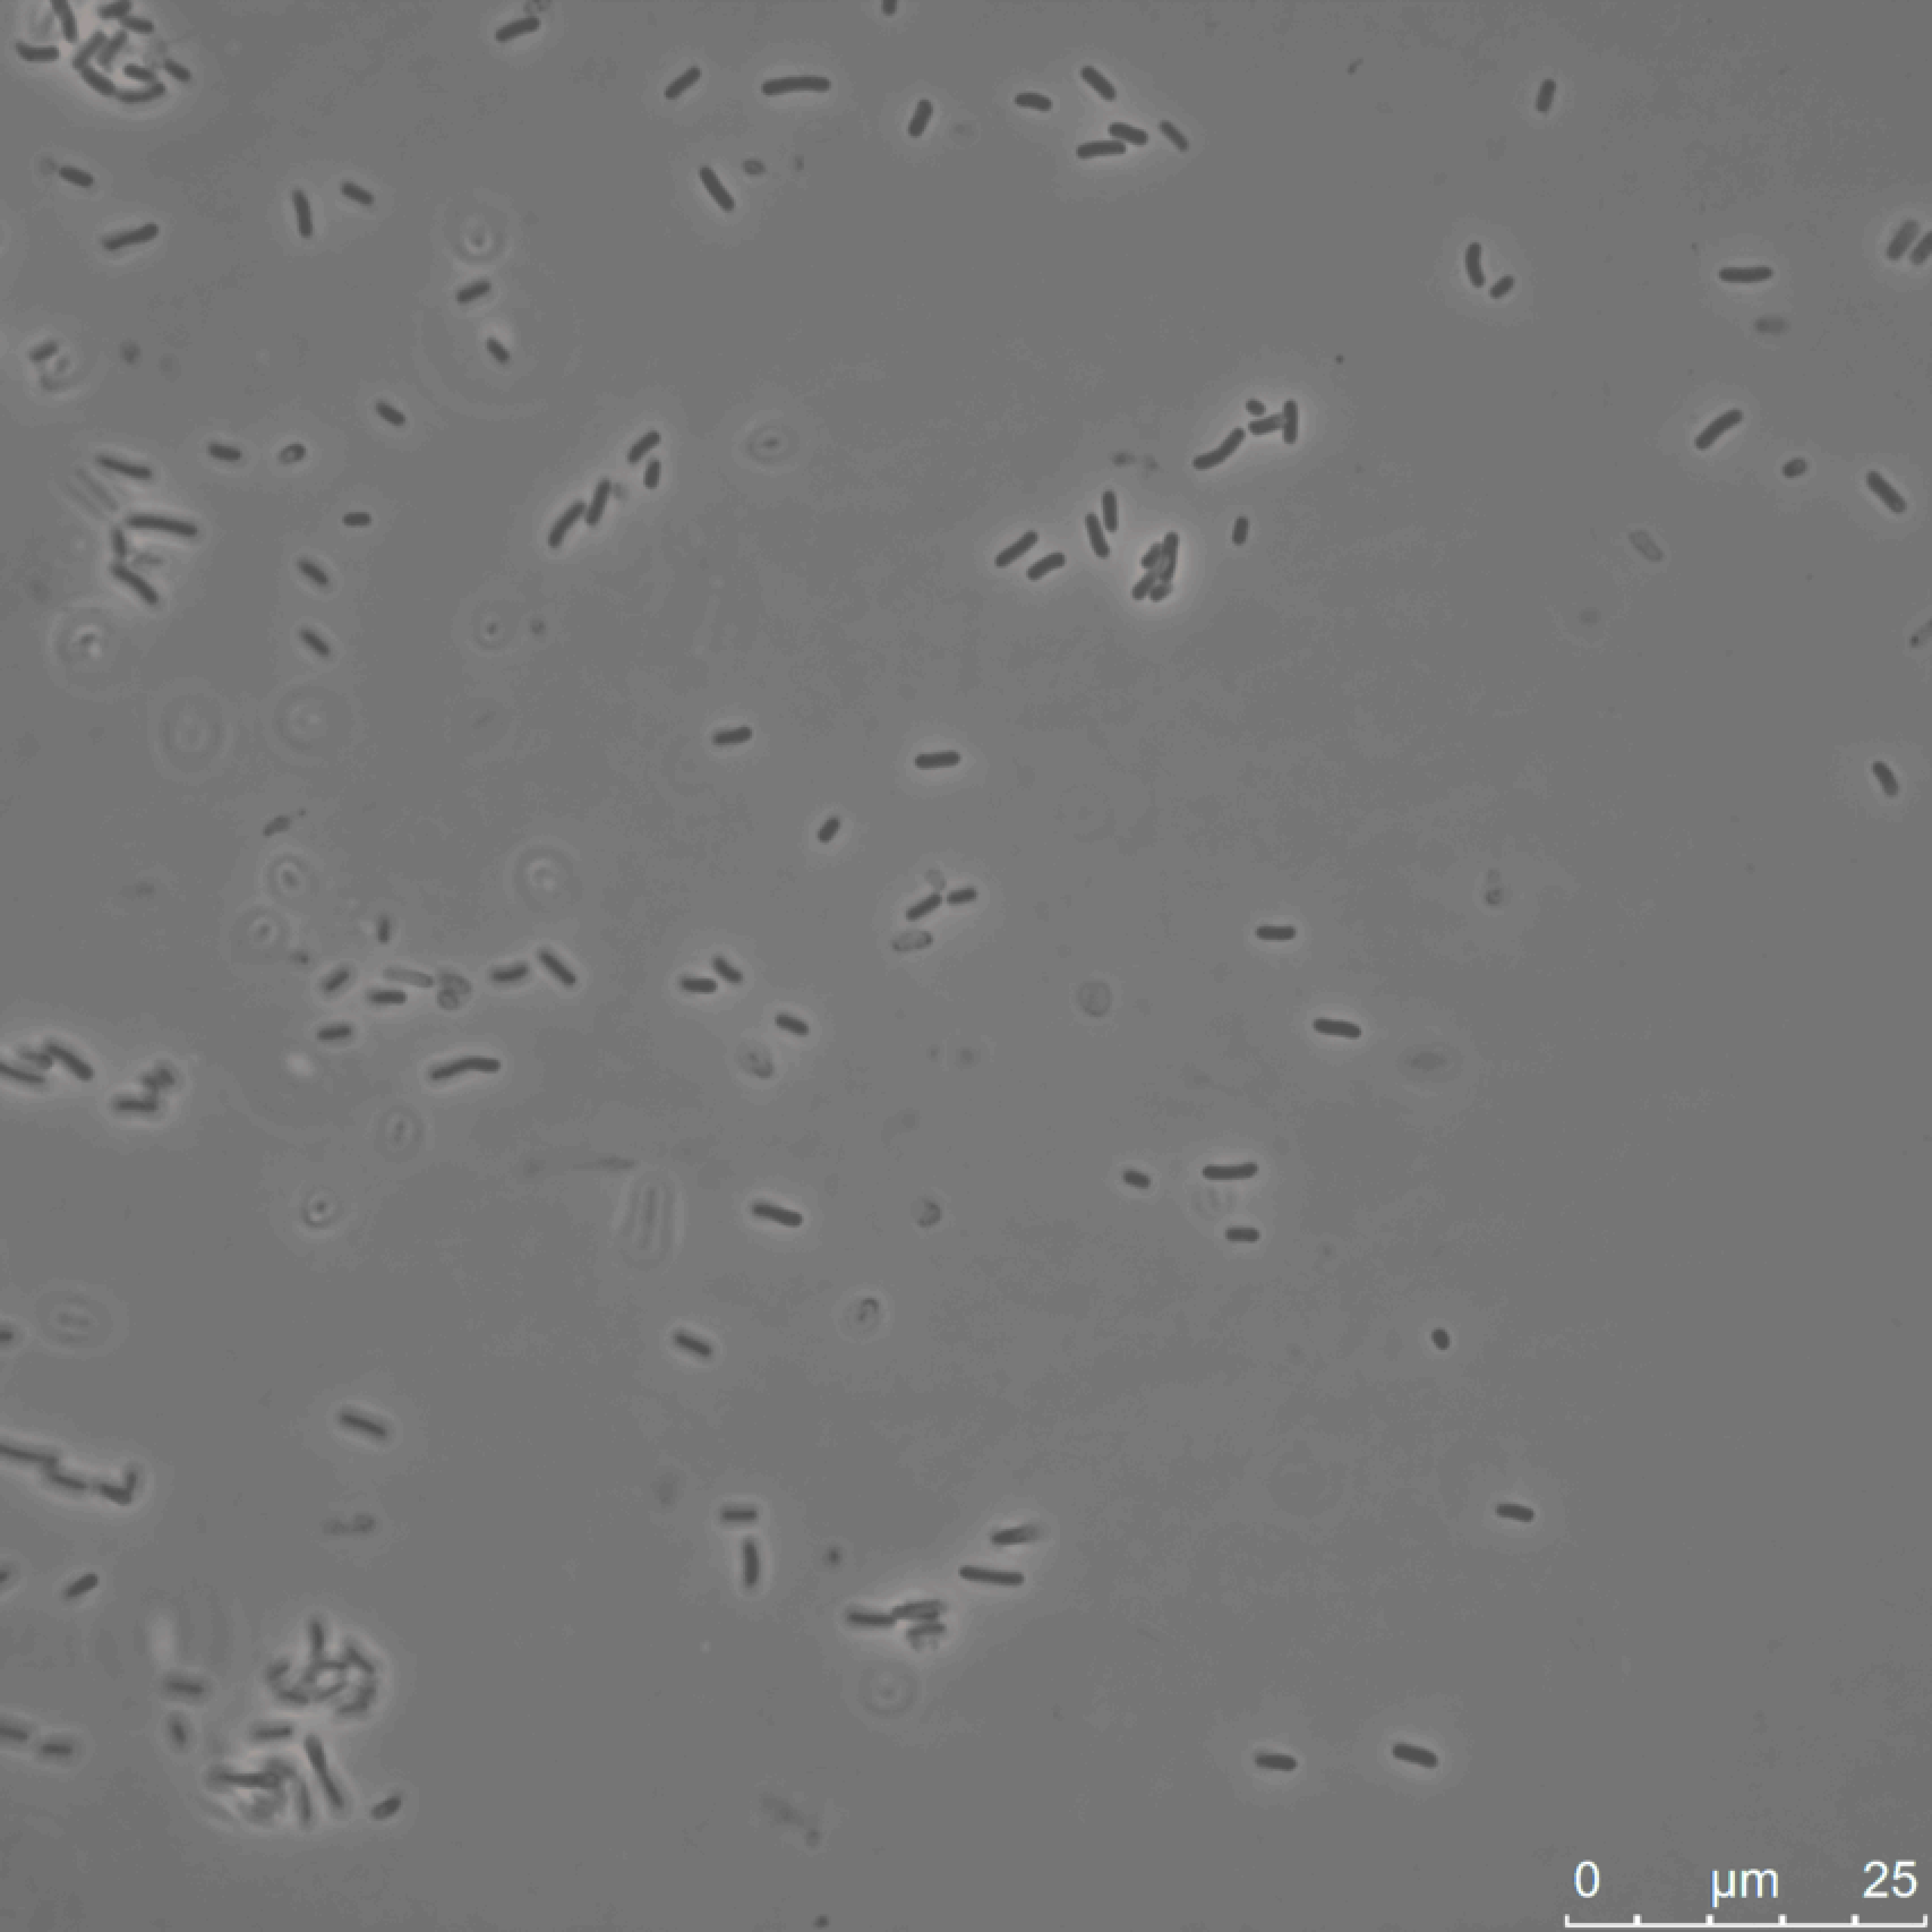
\includegraphics{TT01U1_24HR_3_GREEN-crunch-lighter-resample.pdf} &%
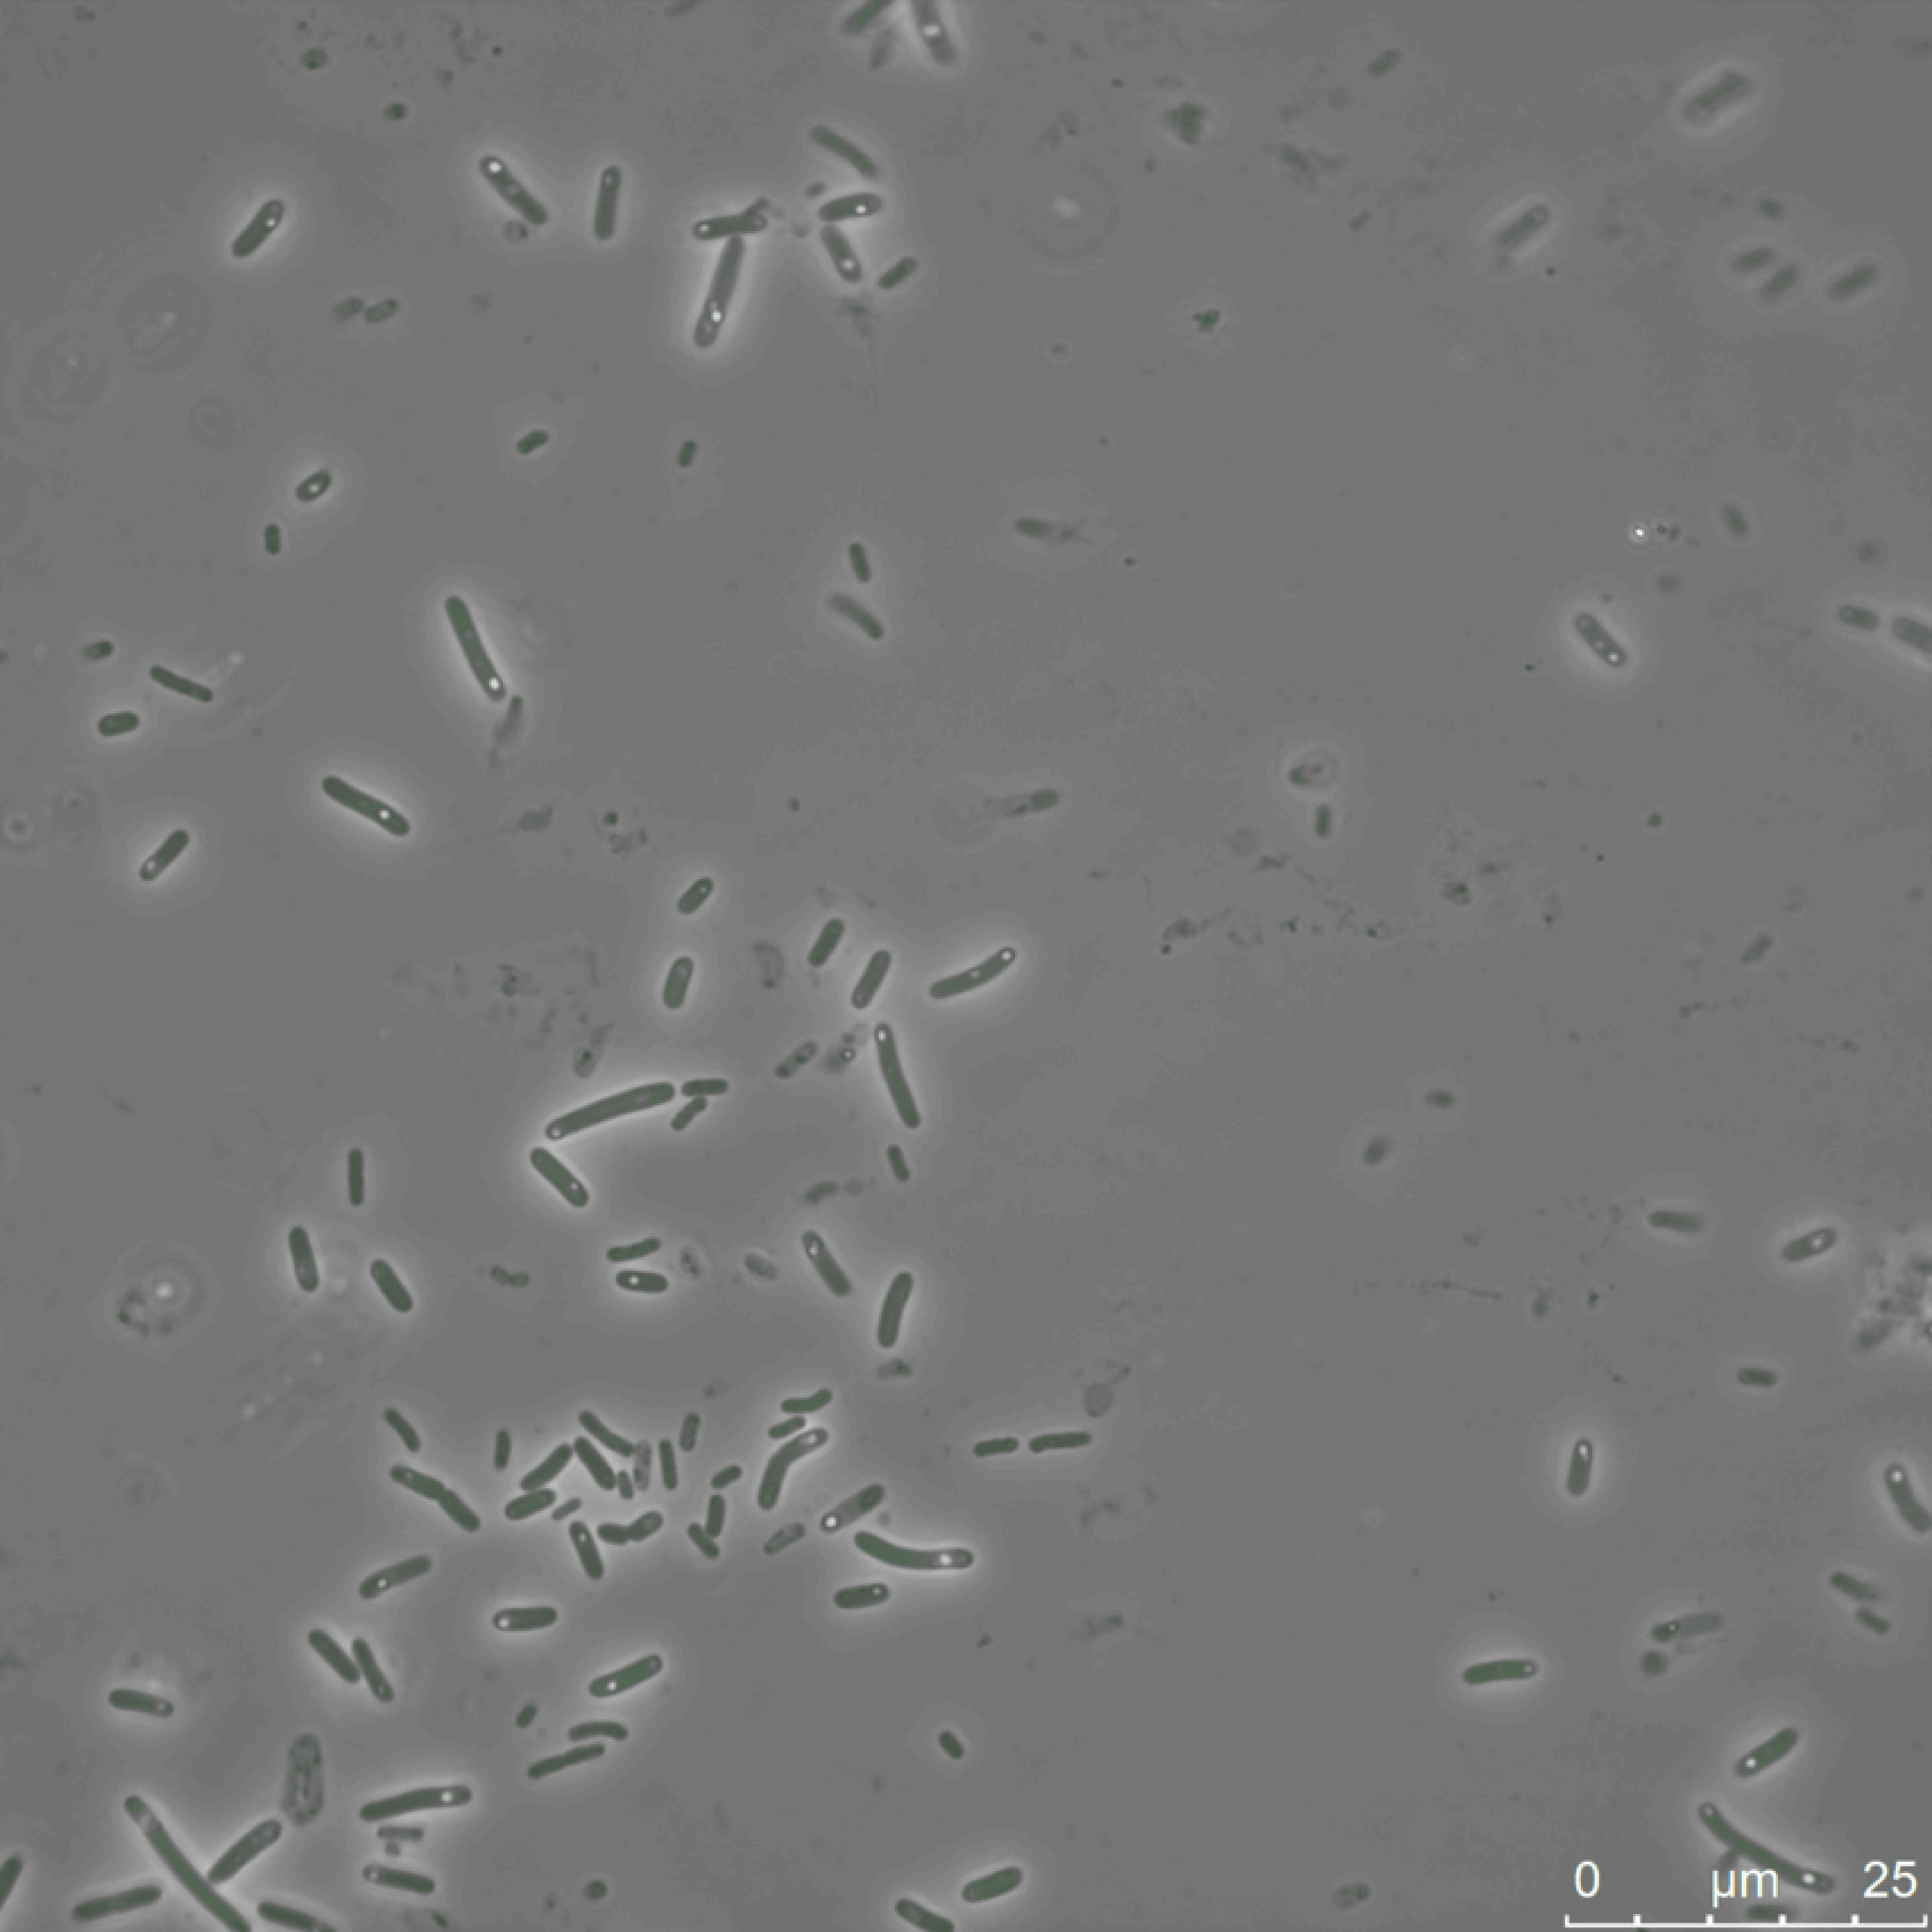
\includegraphics{TT01U1_72HR_3_LOWGREEN-crunch-lighter-resample.pdf} \\[-0.5ex]

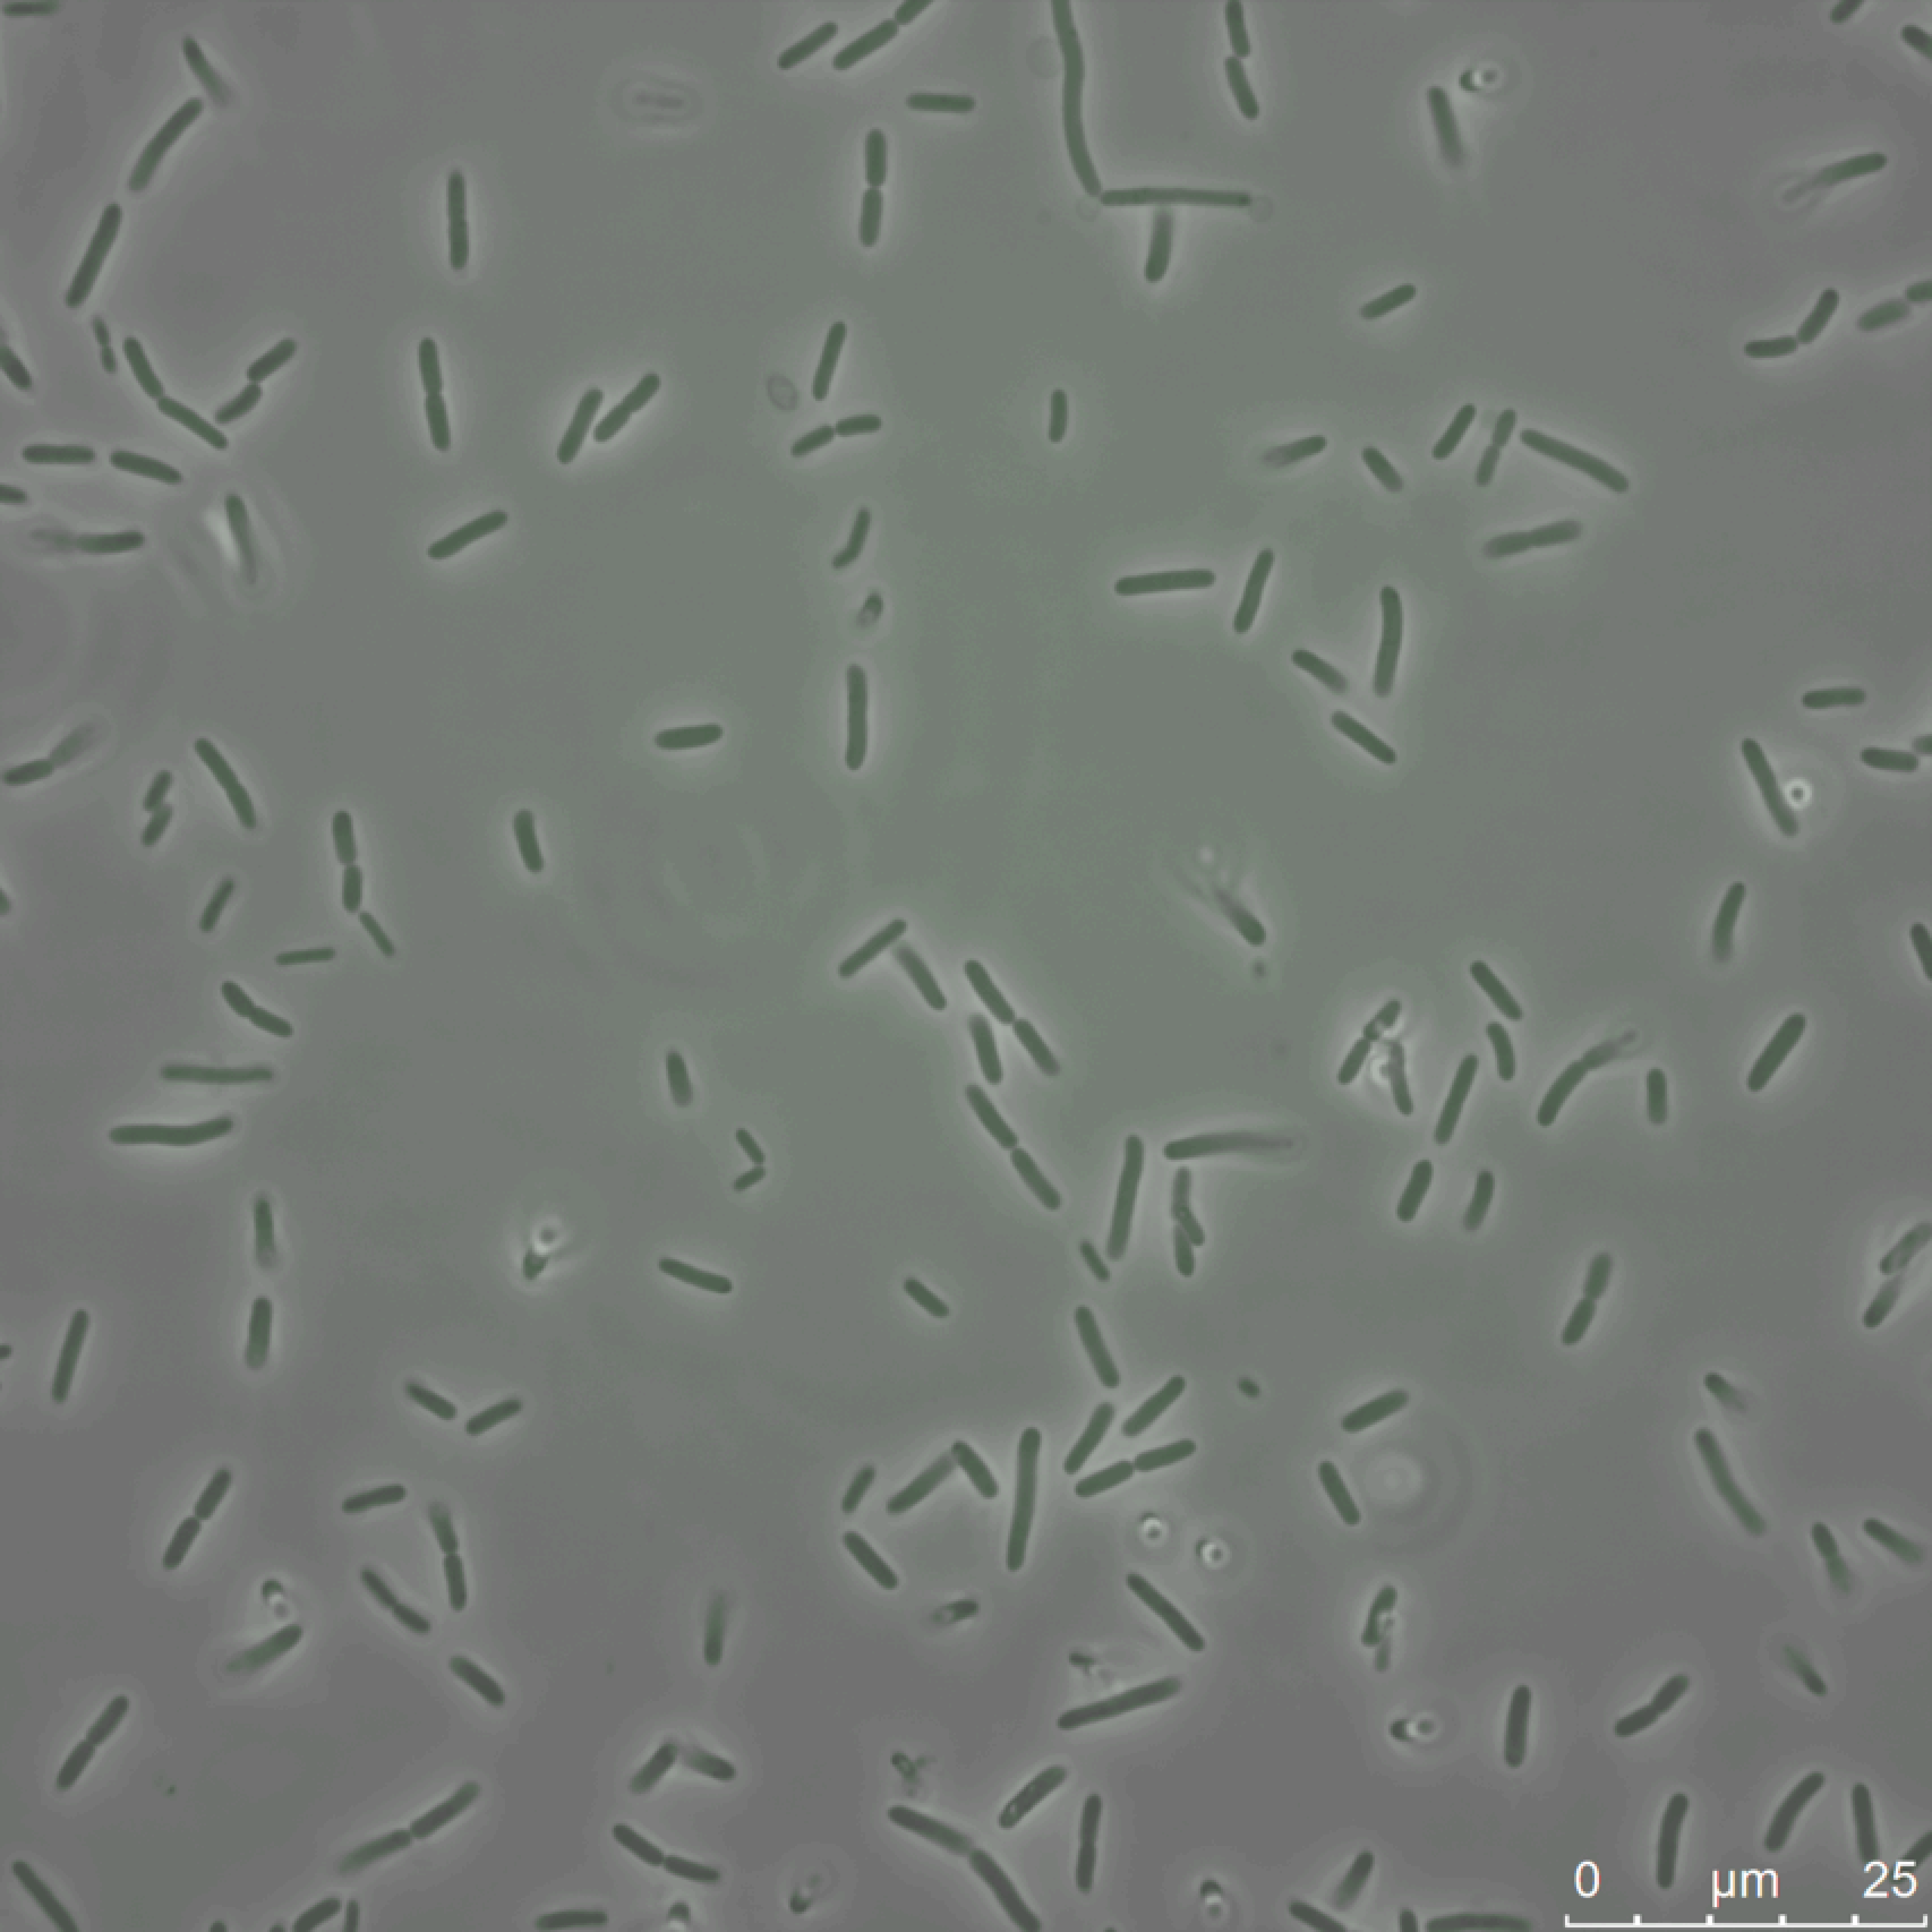
\includegraphics{TT01U1_4_NOGREEN-crunch-lighter-resample.pdf} &%
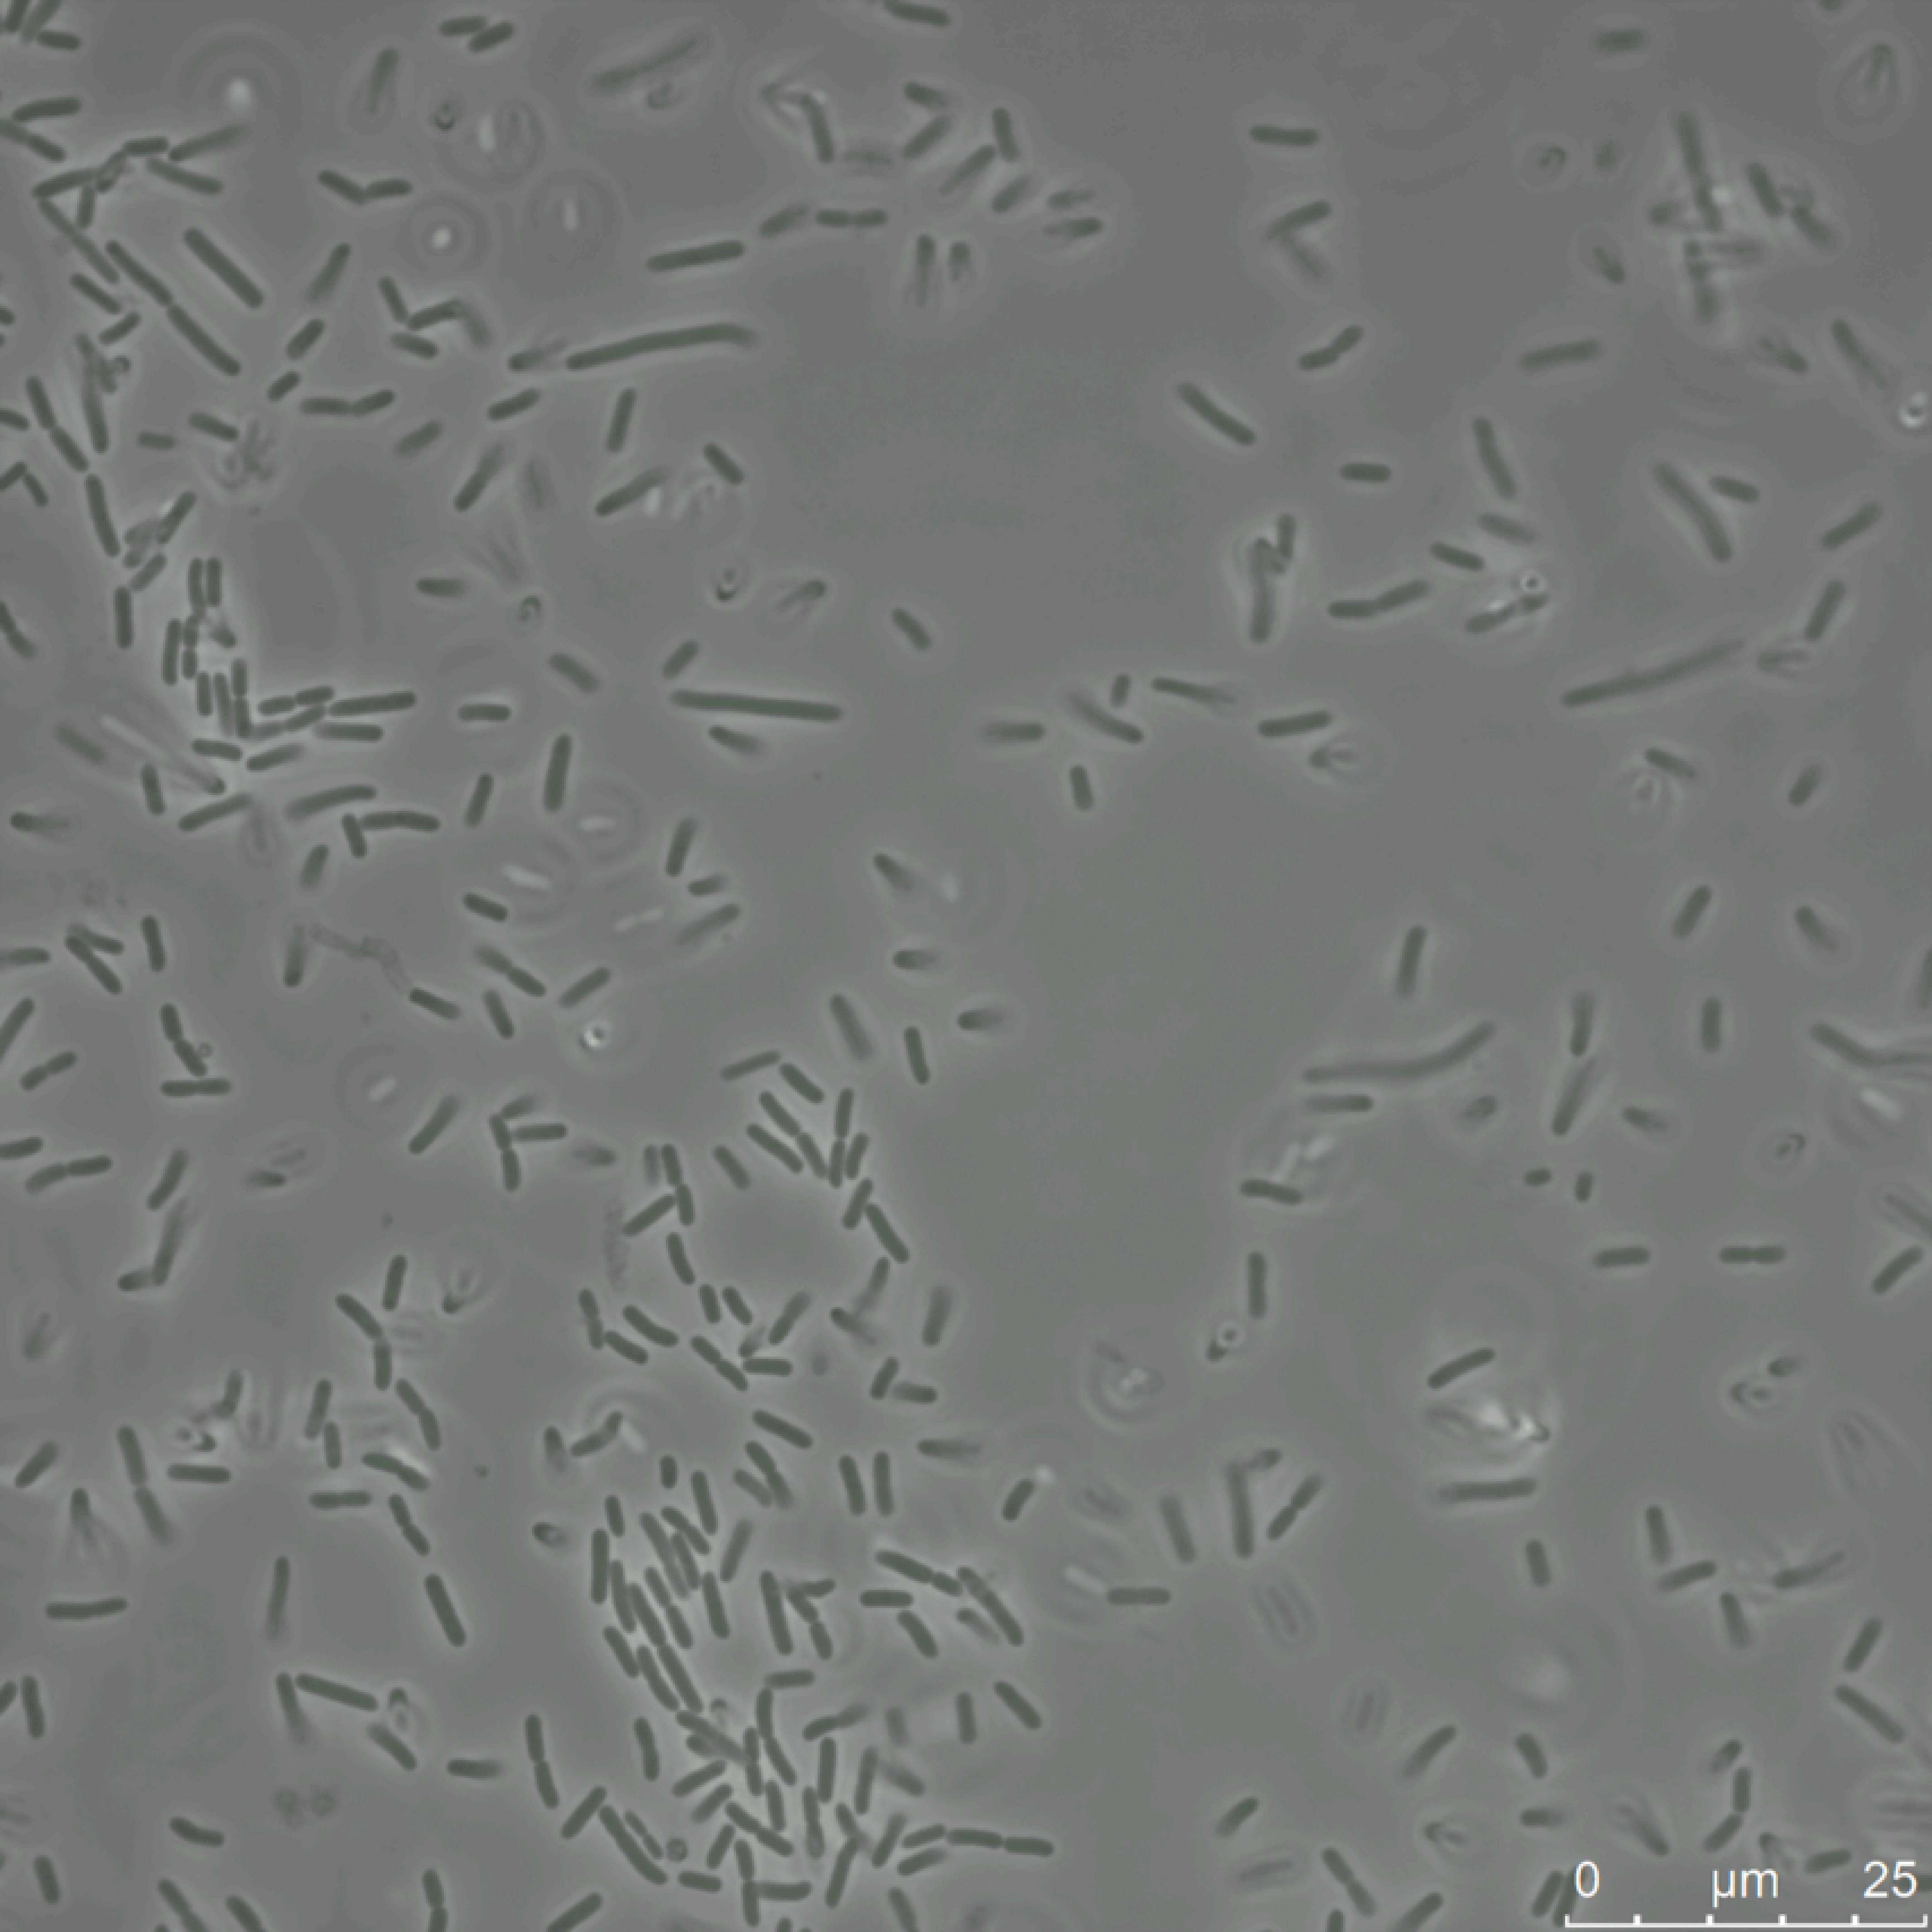
\includegraphics{TT01U1_5HR_4_LOWGREEN-crunch-lighter-resample.pdf} &%
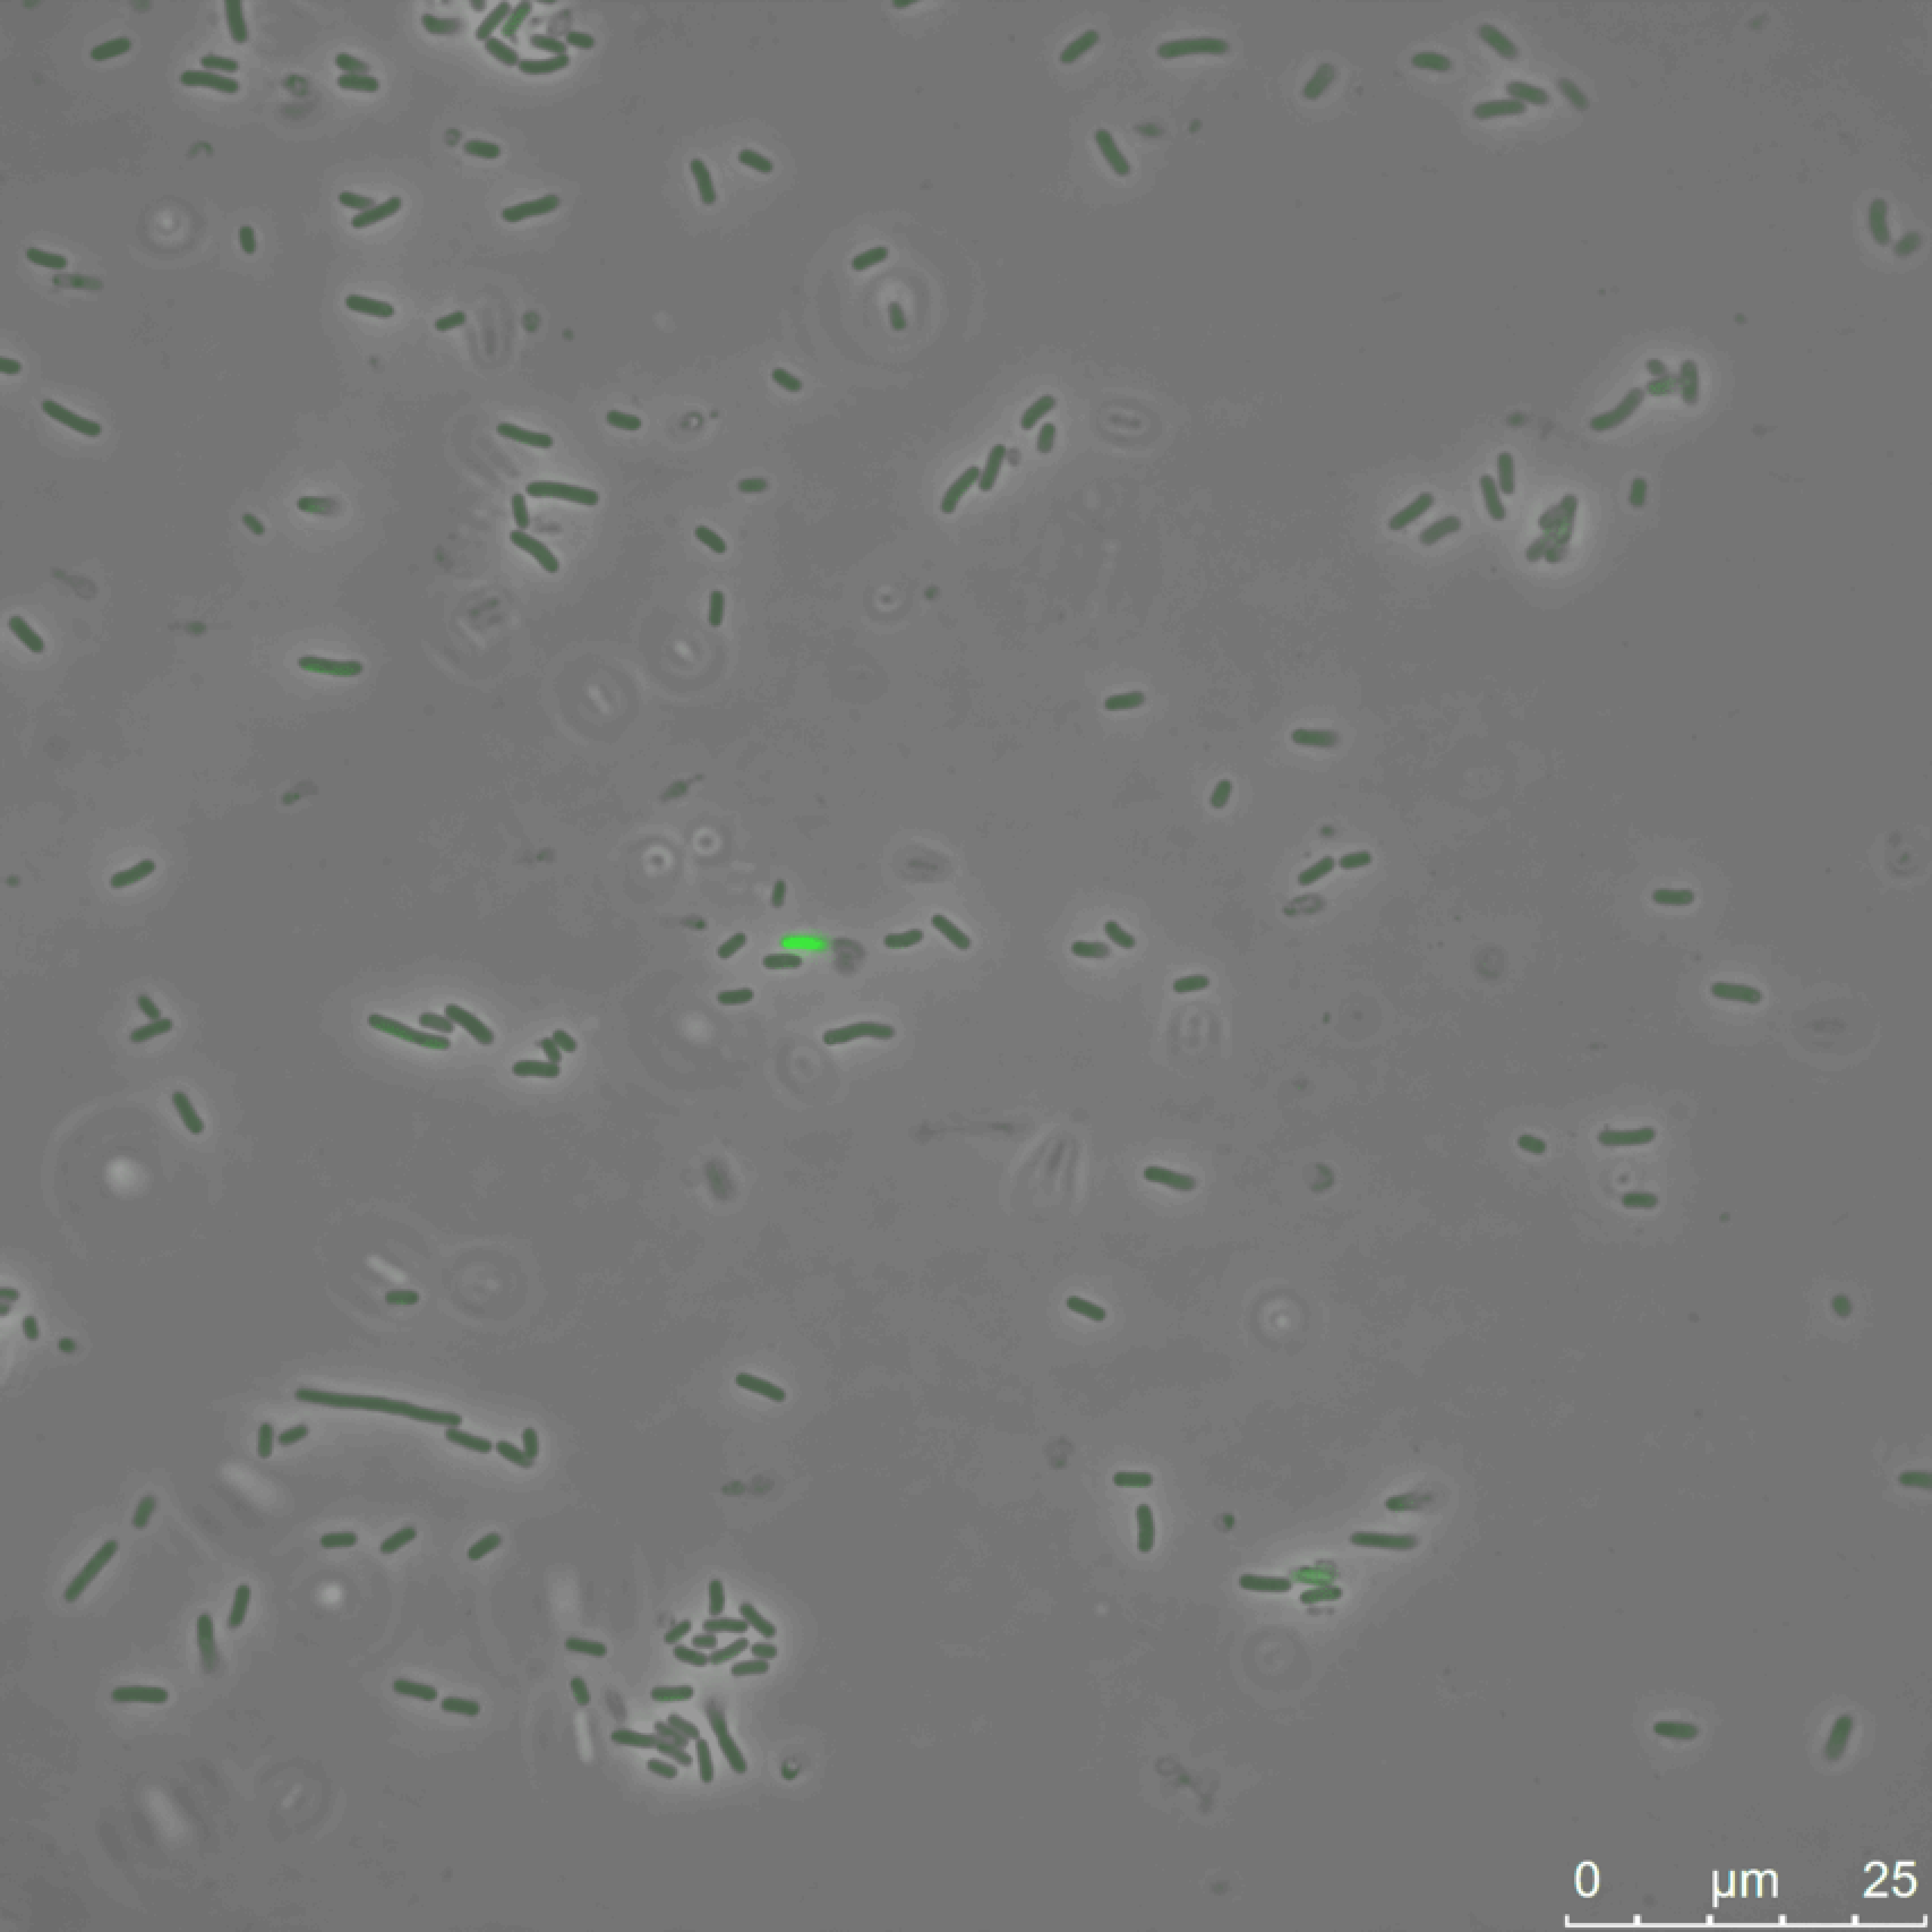
\includegraphics{TT01U1_24HR_4_GREEN-crunch-lighter-resample.pdf} &%
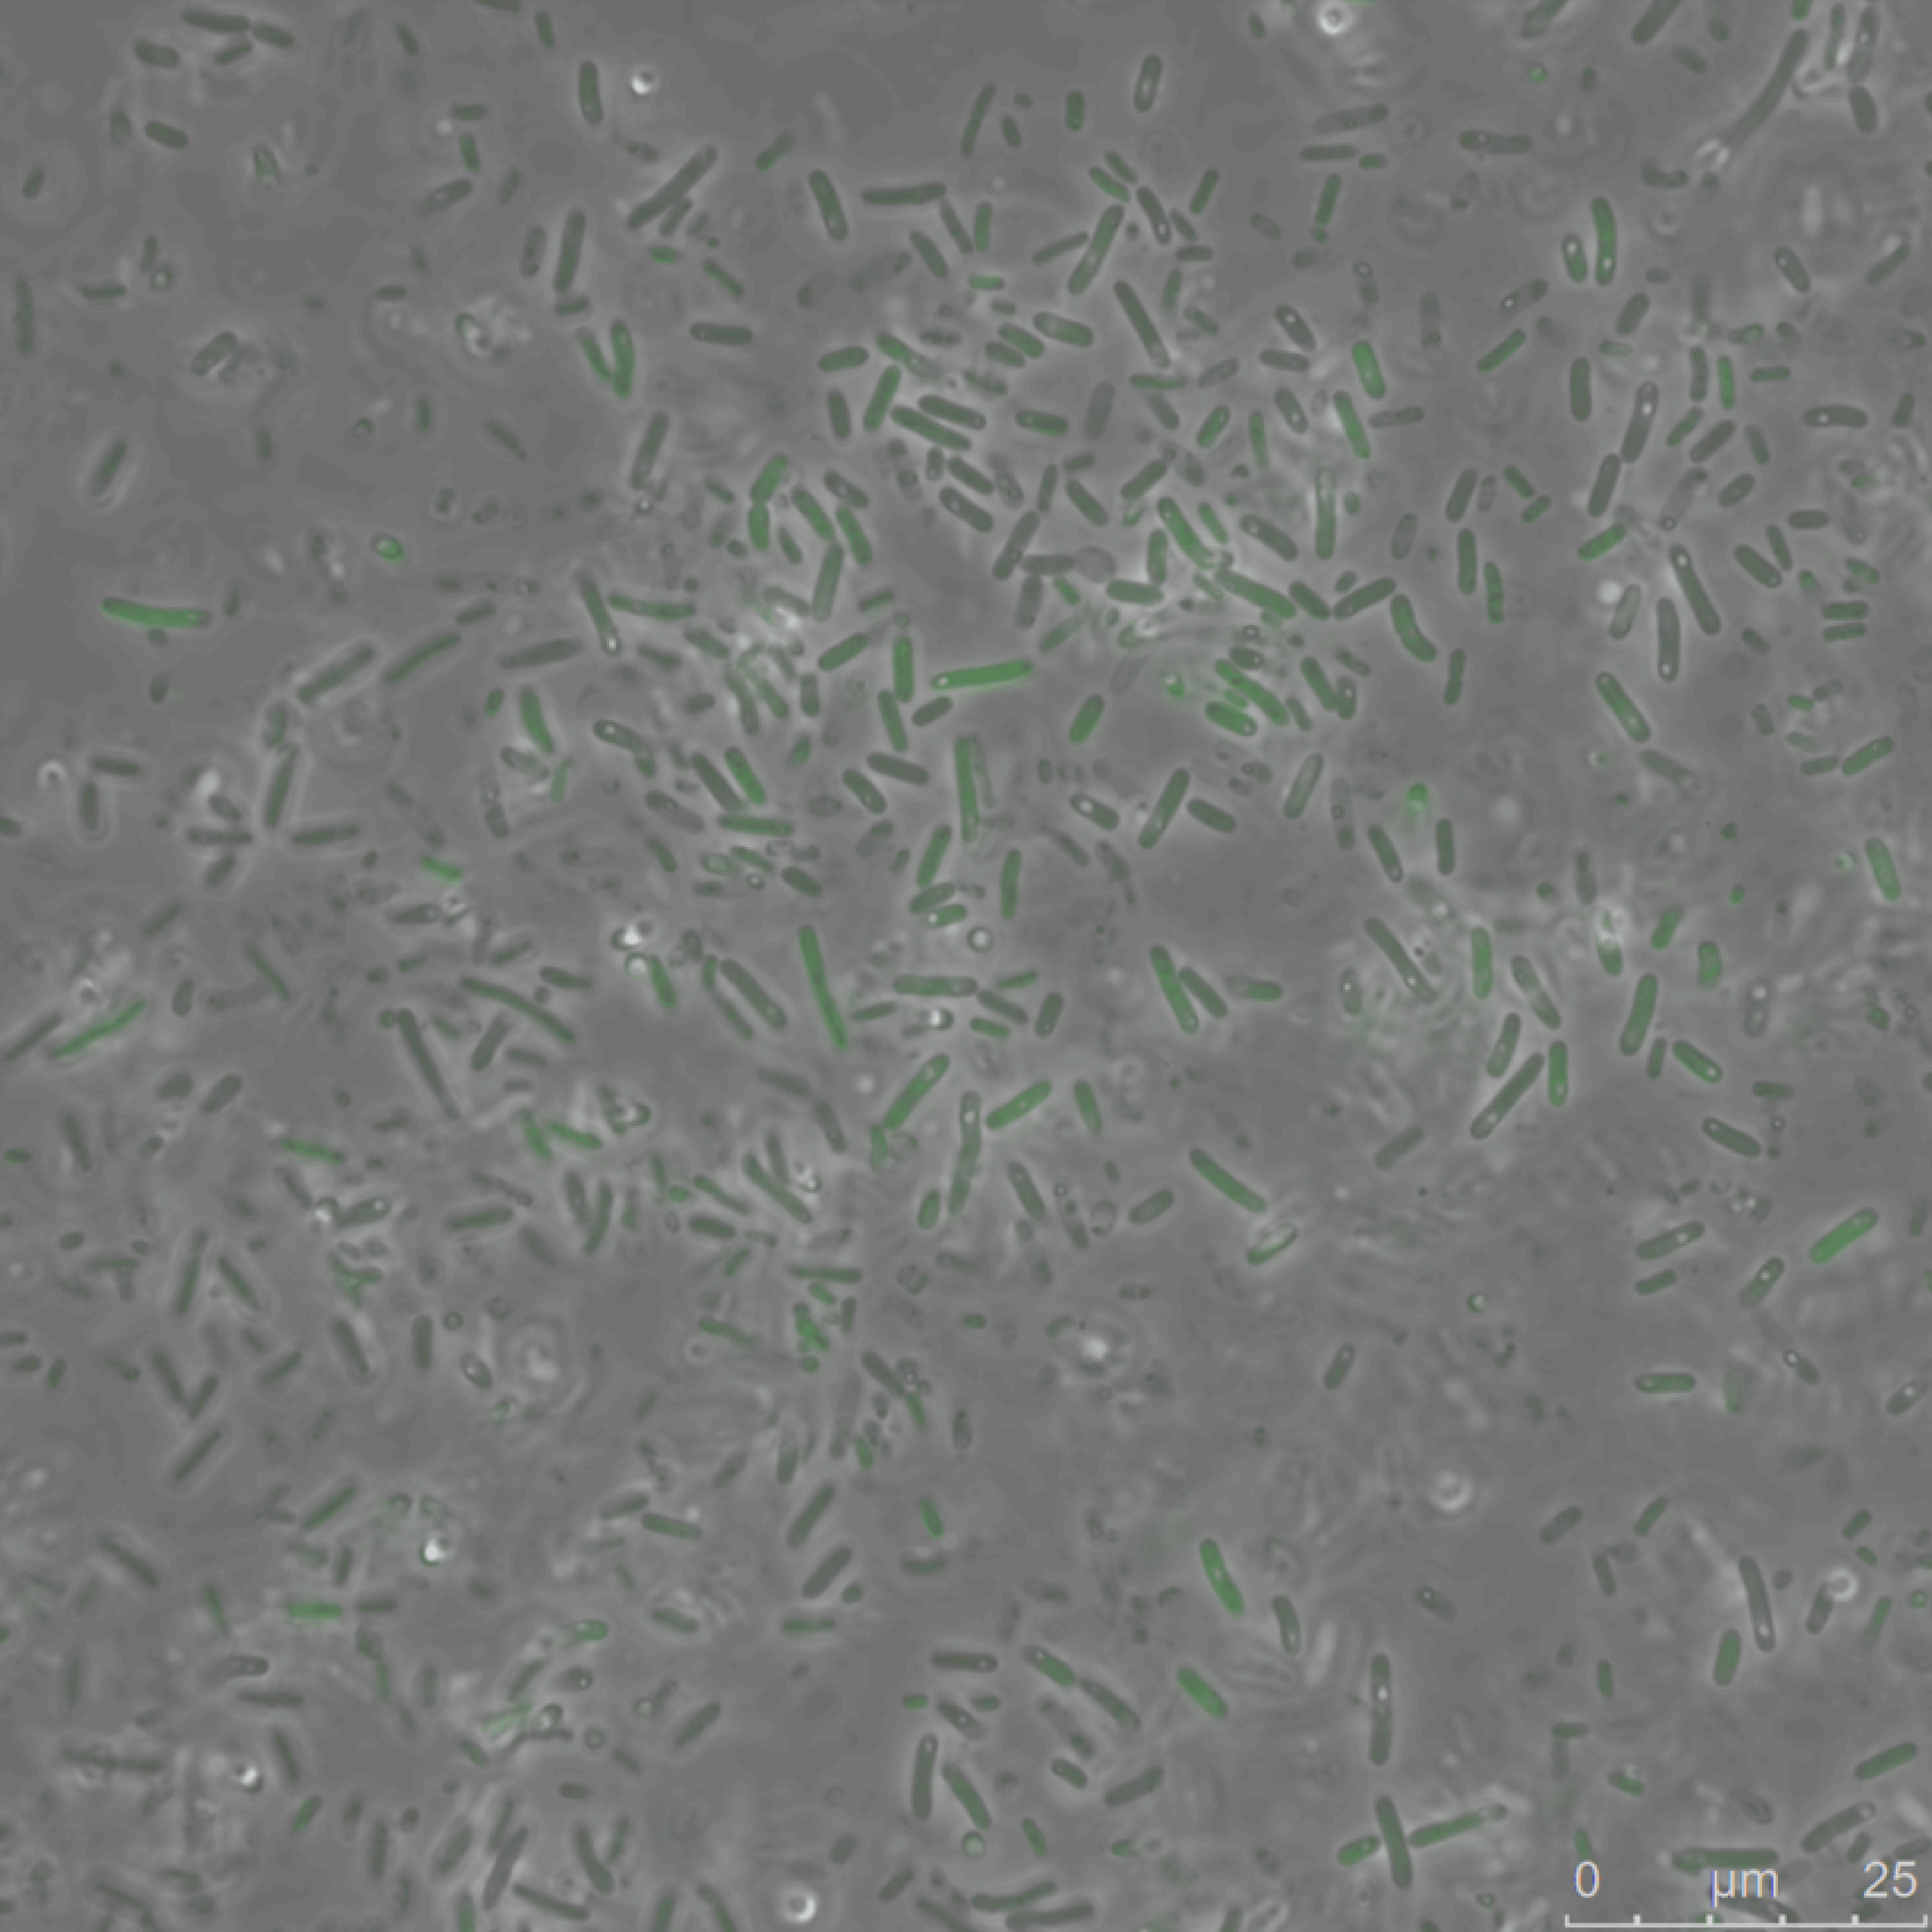
\includegraphics{TT01U1_72HR_5_GREEN-crunch-lighter-resample.pdf} \\
 - & - &  ++ & ++ \\[1ex]

\end{tabularx}

\captionsetup{singlelinecheck=off, justification=justified, font=footnotesize, aboveskip=20pt}
\caption[Reporter microscopy - TT01 Unit 1]{\textsc{\normalsize Reporter microscopy for the \emph{P. luminescens} TT01 ``Unit 1" promoter.}\vspace{0.1cm} \newline A representative selection of images for 4 time points, for the PVC ``Unit 1" promoter fusion. Quadruplicate images are displayed vertically as representative of the whole slide sample. Key to qualitative fluorescence indication: ``-" - no fluorescence, ``+" - low level fluorescence in isolated cells. ``++" - low level fluorescence in many cells or few brighter cells, ``+++" - intermediate to high fluorescence in almost all cells, or very bright isolated cells.}
\end{figure}\label{RMTT01U1}
\endgroup

%%%%%%%%%%%%%%%%%%%%%%%%%%%%%%%%%%%%%%%%%%%%%%%%%%%%%%%%%%%%%%%%%%%%

\begingroup
\renewcommand{\arraystretch}{0.8}%
\setlength{\tabcolsep}{0.3pt}
\begin{figure}[p]
\setkeys{Gin}{width=\linewidth}
\Huge
\begin{tabularx}{\textwidth}{CCCC}
\multicolumn{4}{p{\linewidth}}{\large \centering \textbf{\emph{P. asymbiotica} PB68.1 (``THAI") PVC ``Unit 1"}} \\
\hiderowcolors
& & & \\[-1.5ex]
\Large 2 Hours &\Large 5 Hours &\Large 24 Hours &\Large 72 Hours \\[1ex]

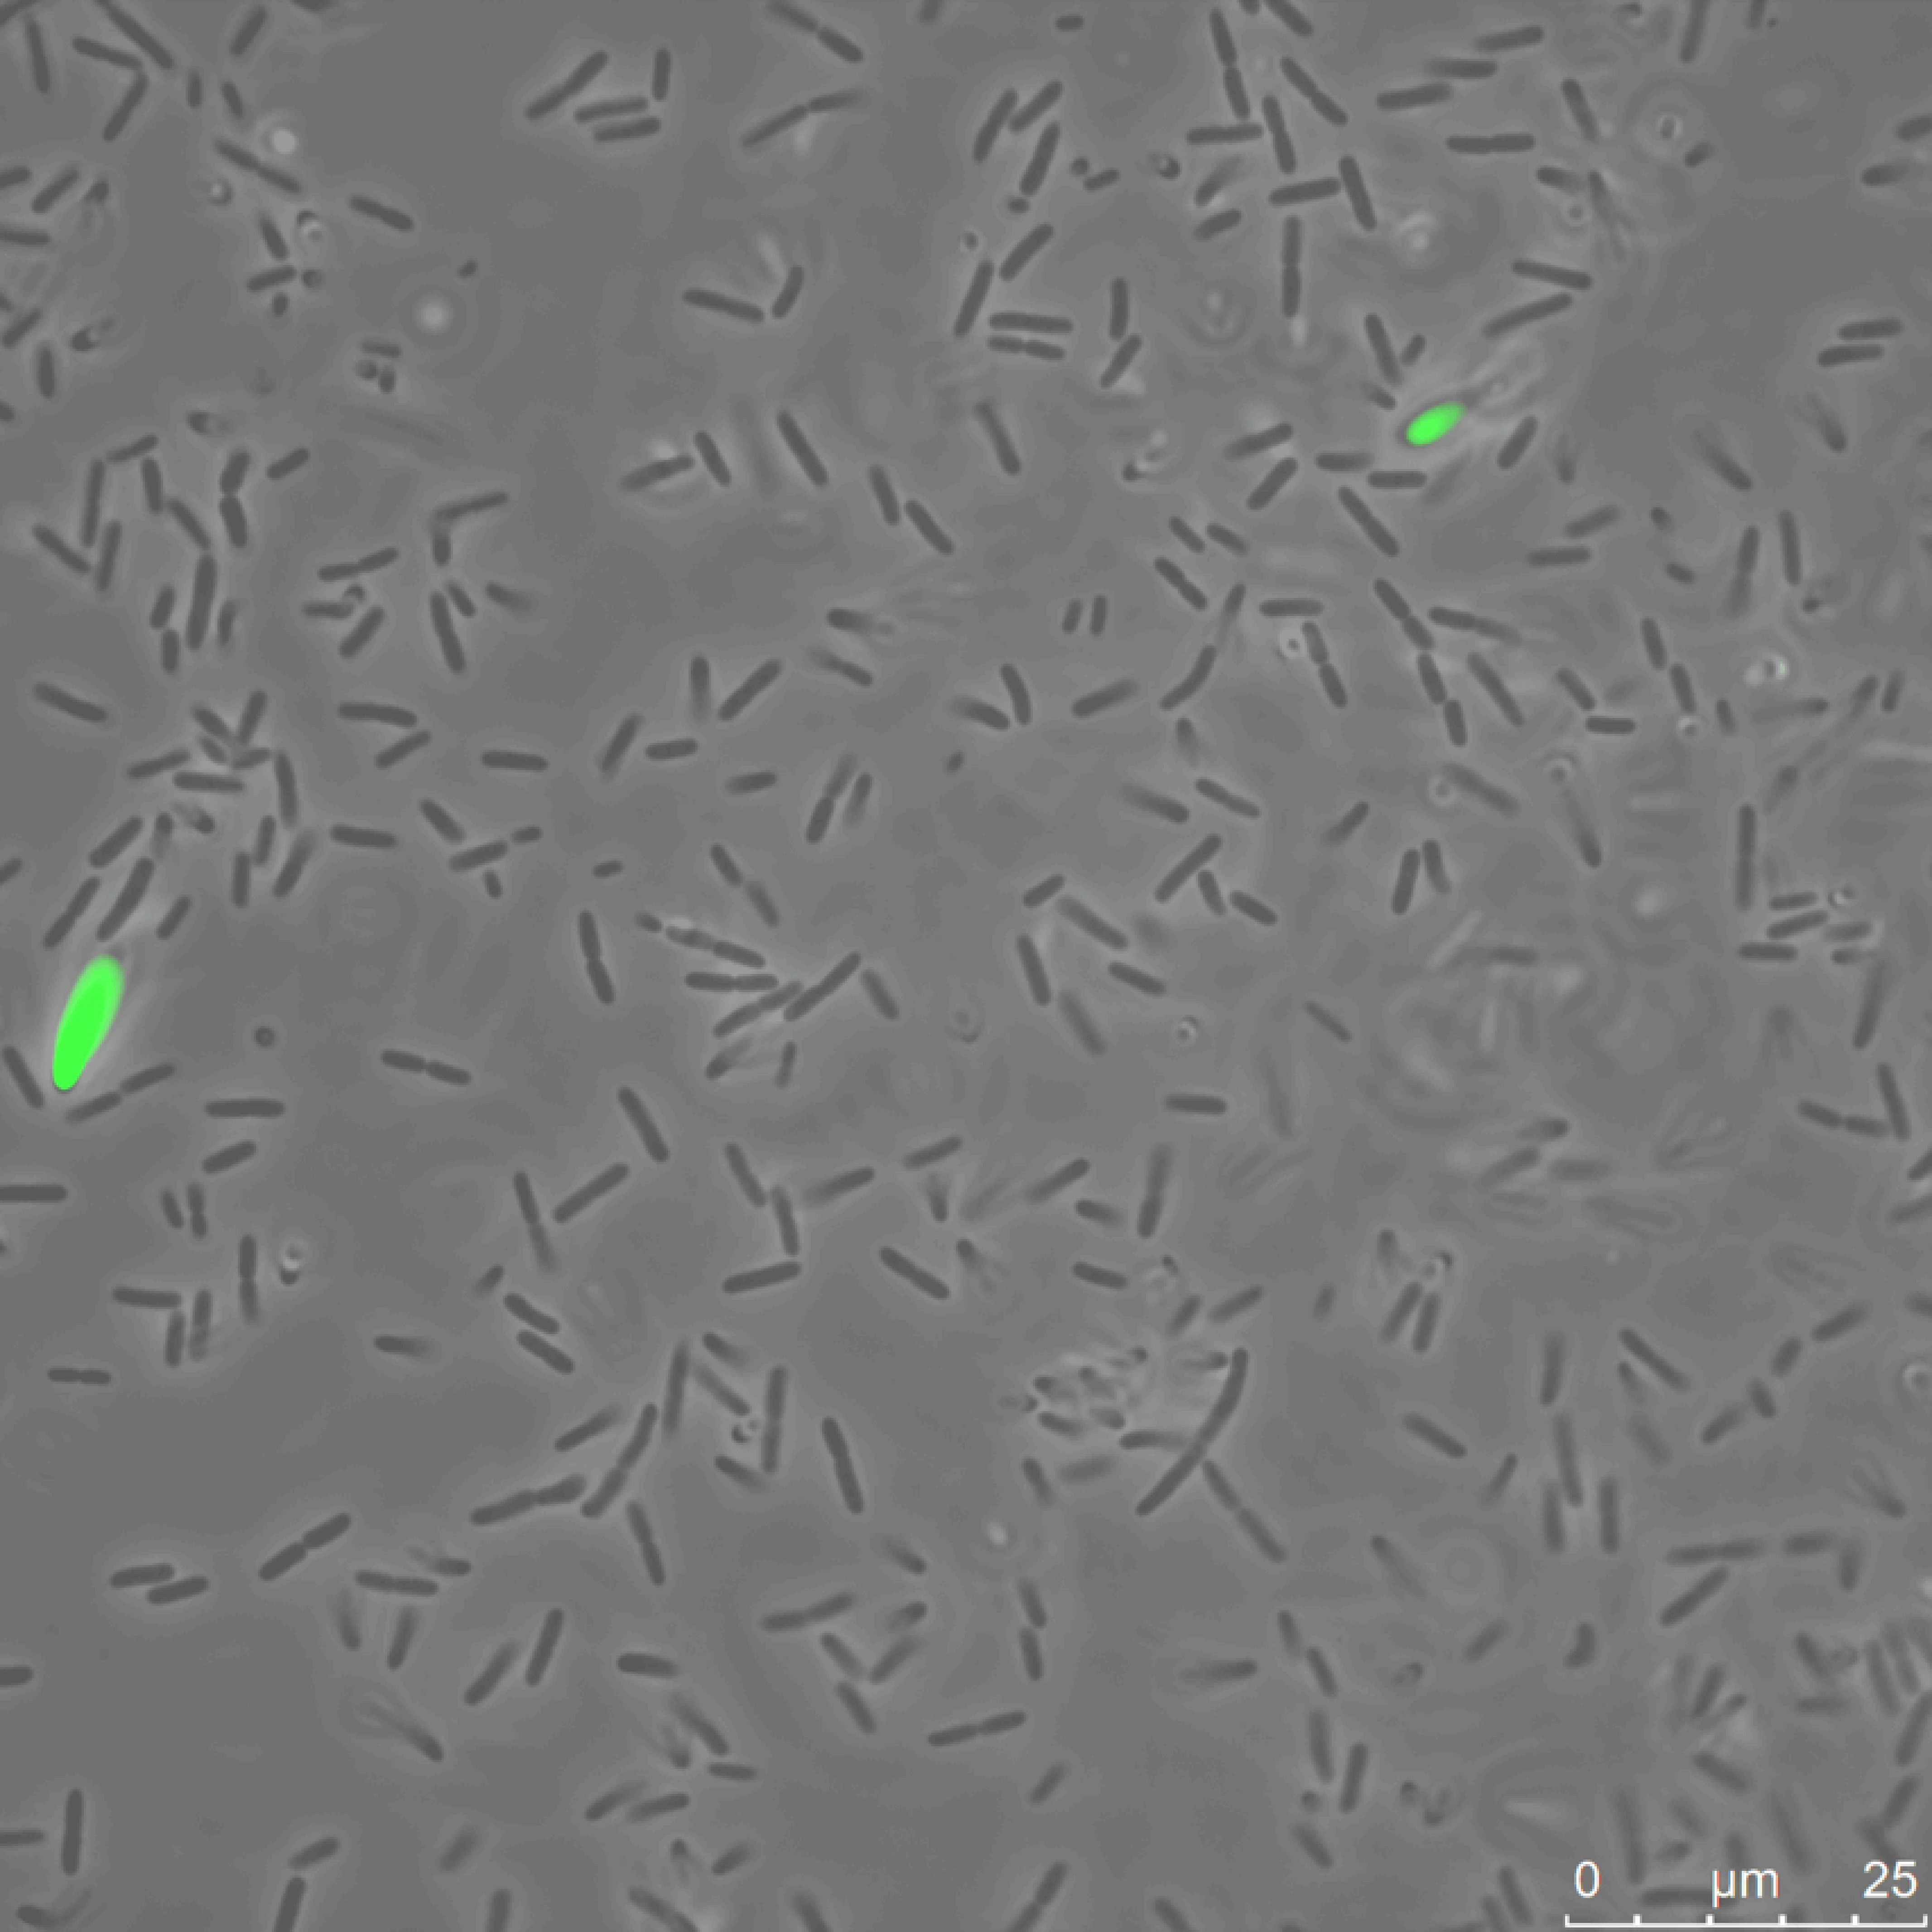
\includegraphics{THAIU1_1_GREEN-crunch-lighter-resample.pdf} &%
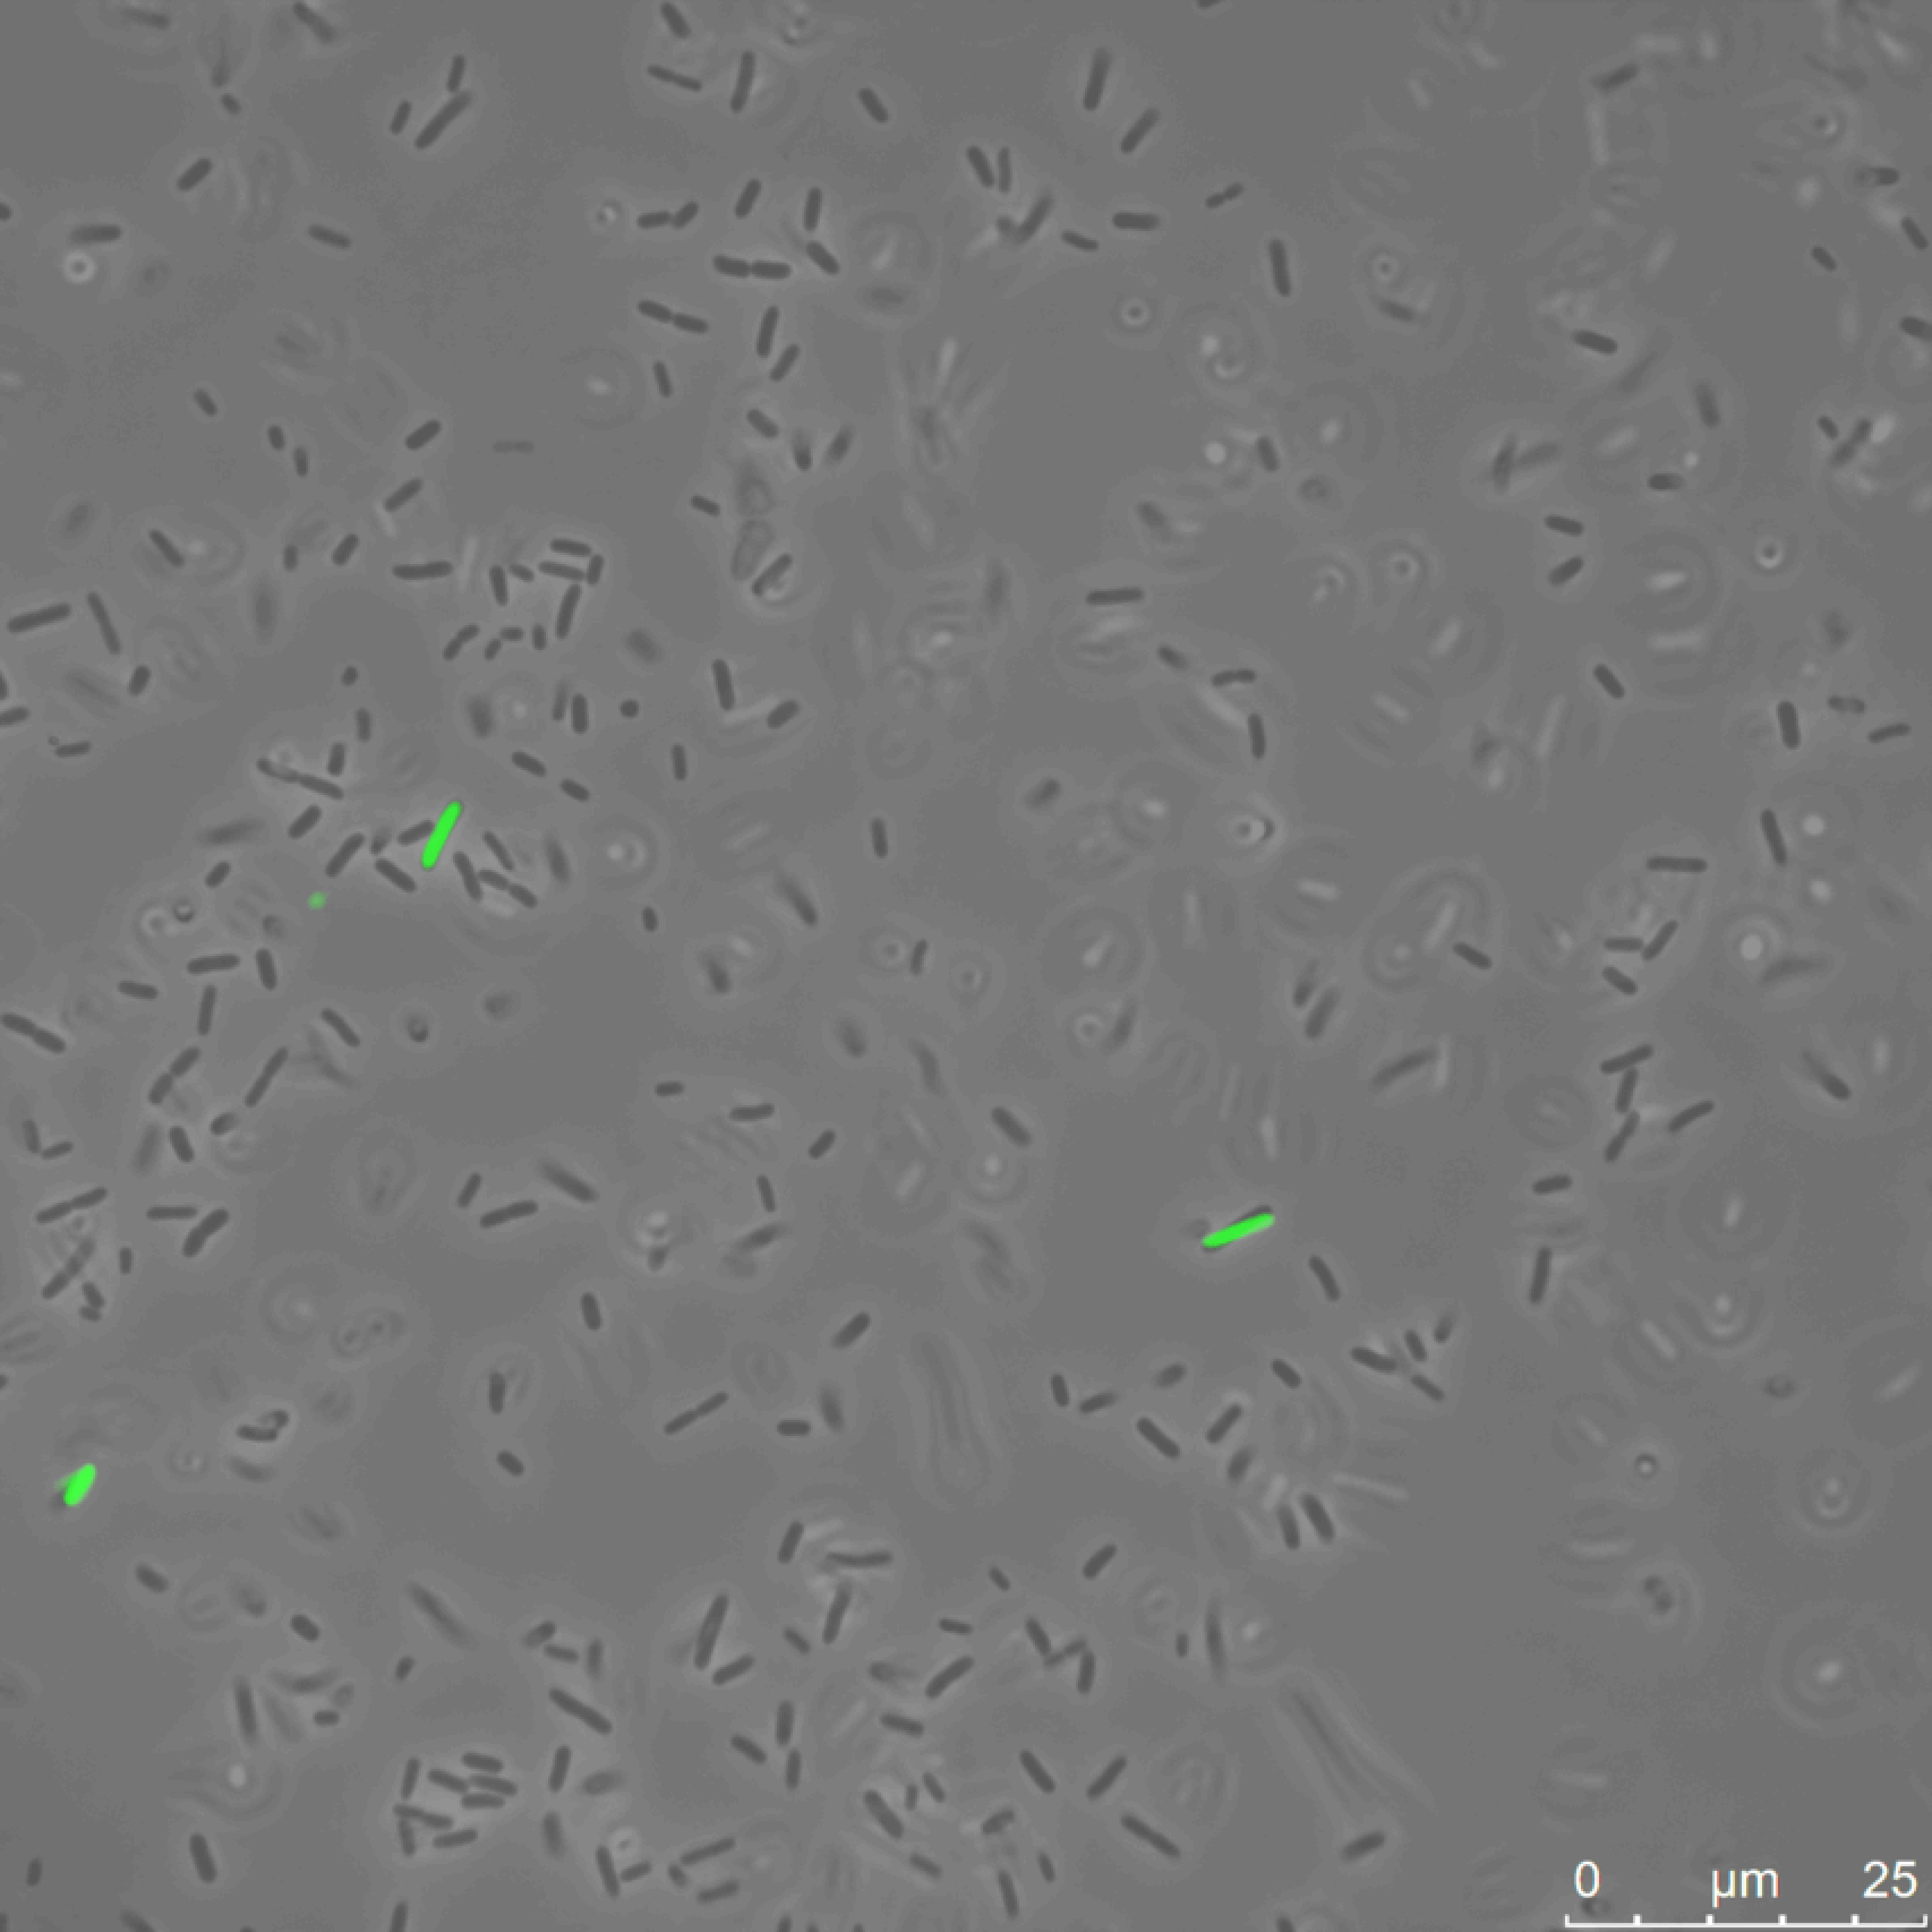
\includegraphics{THAIU1_5HR_5_GREEN-crunch-lighter-resample.pdf} &%
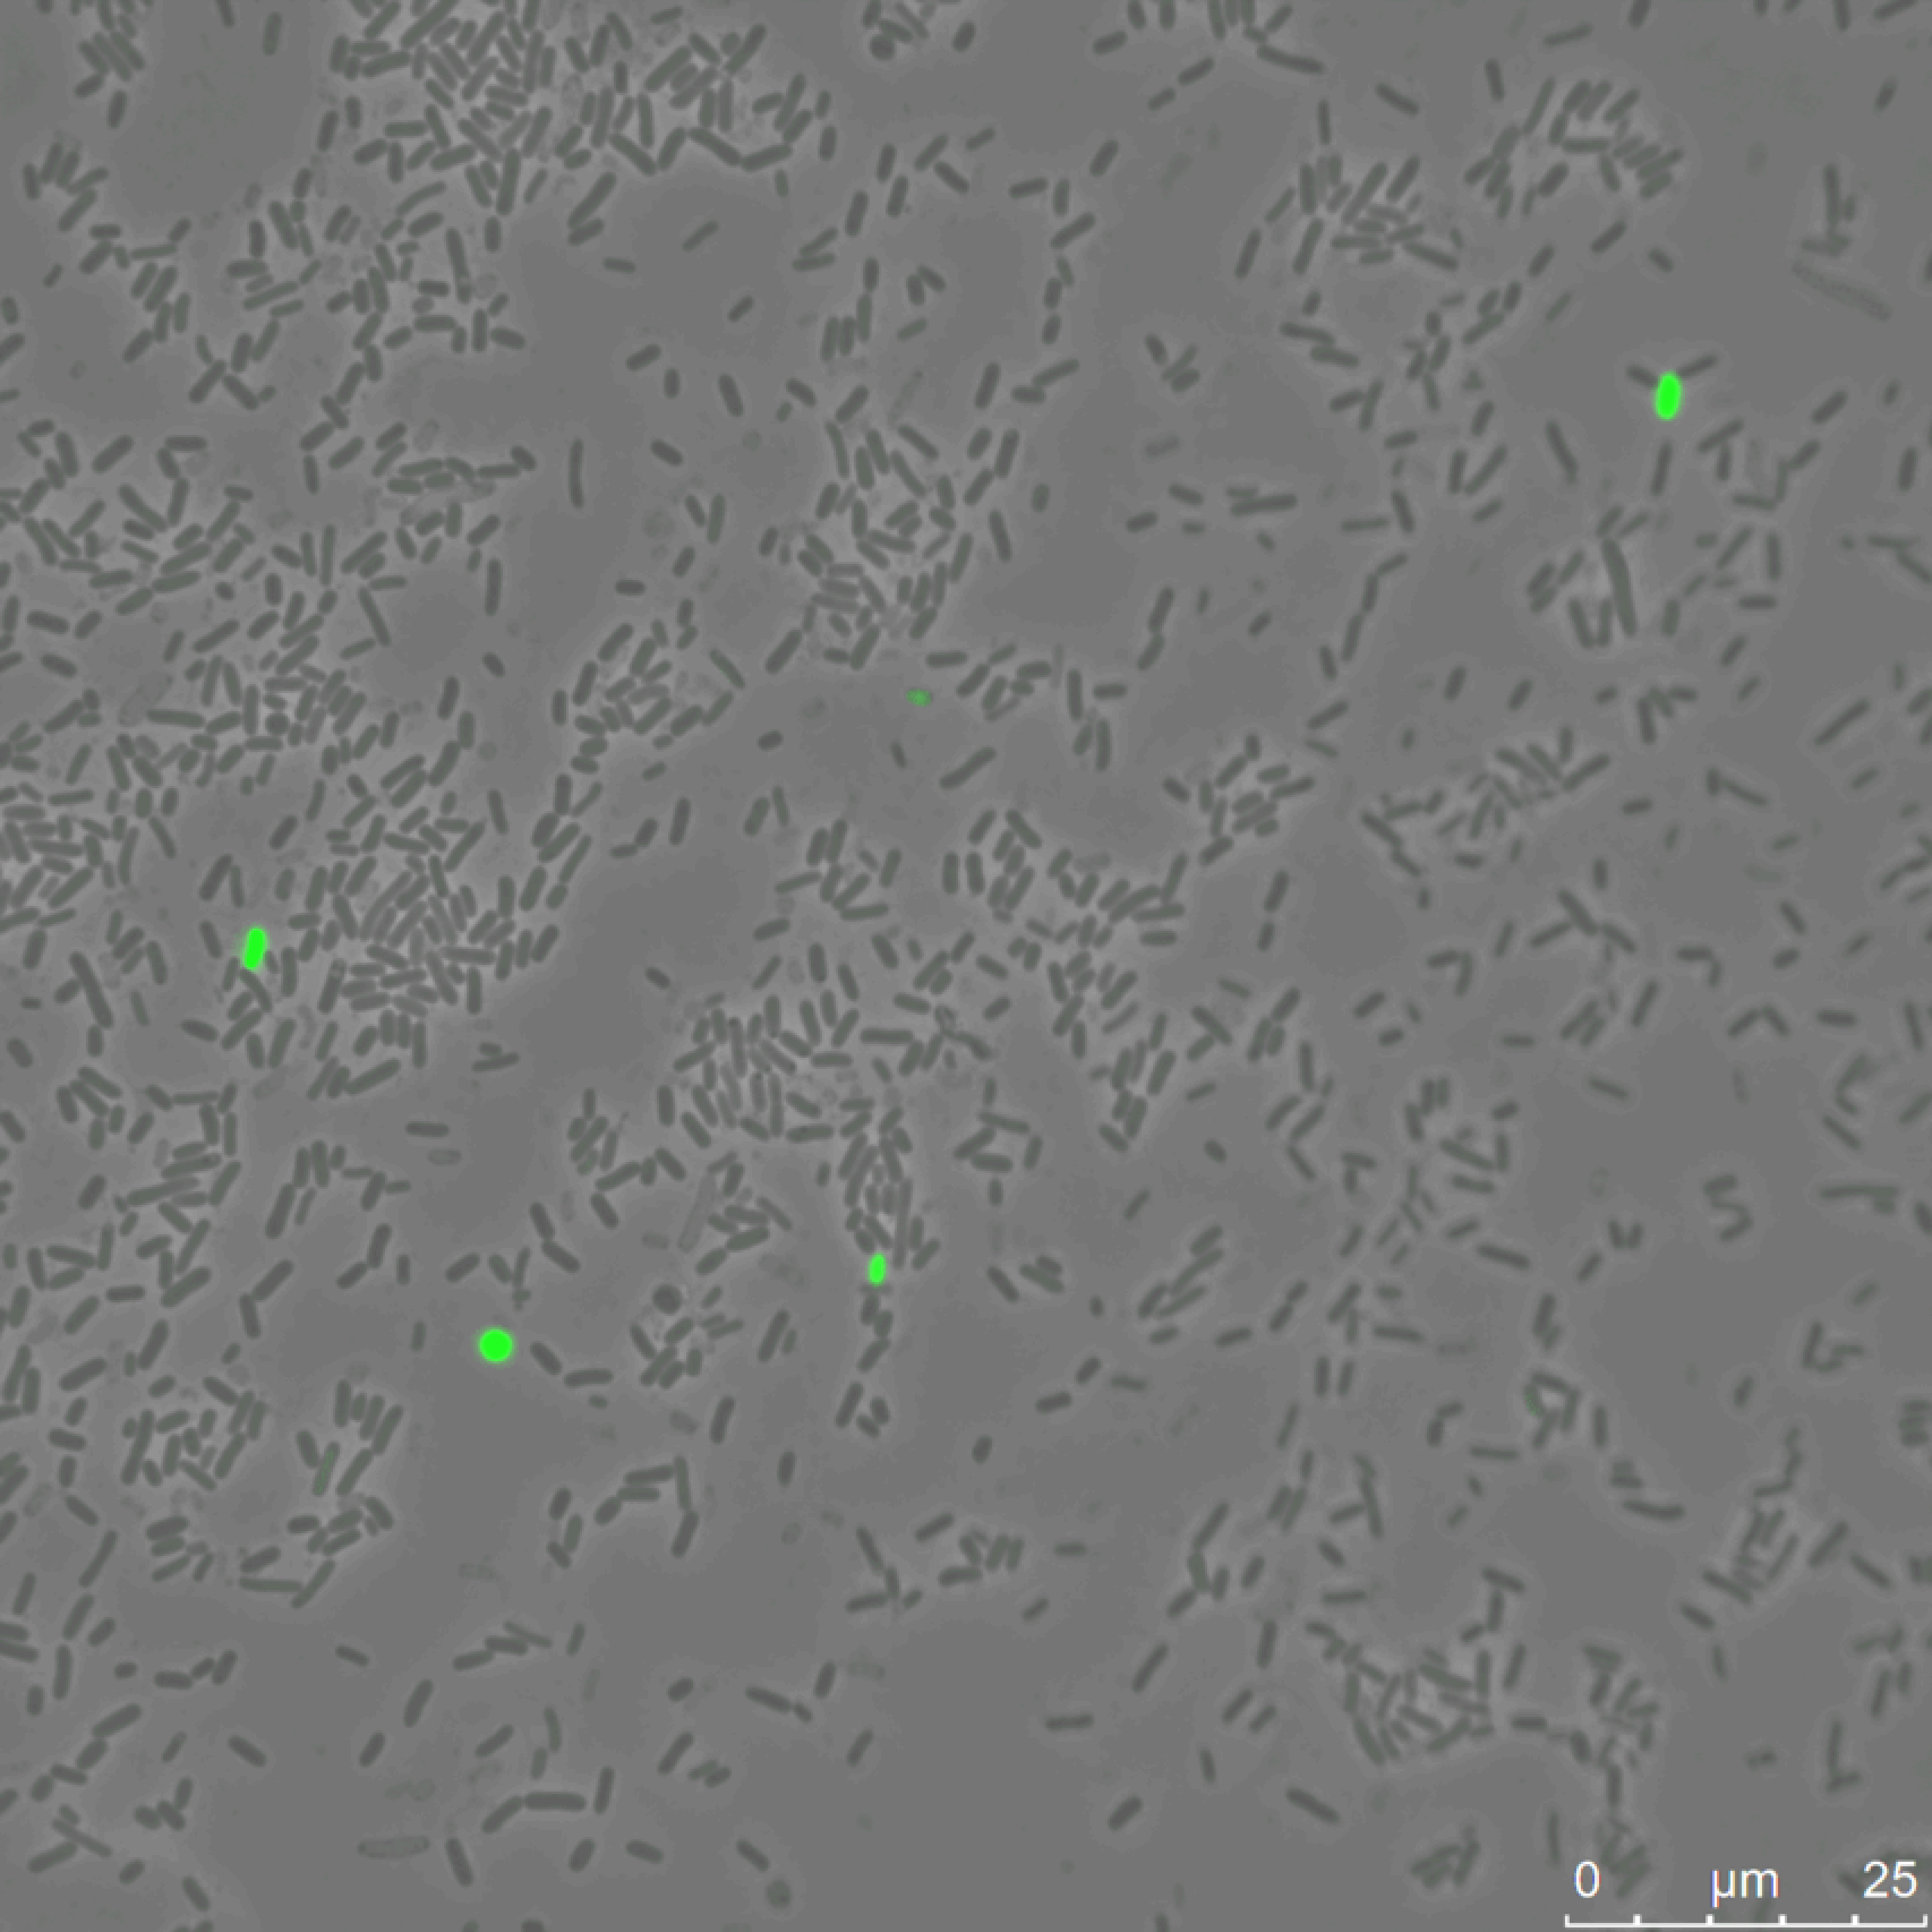
\includegraphics{THAIU1_24HR_1_GREEN-crunch-lighter-resample.pdf} &%
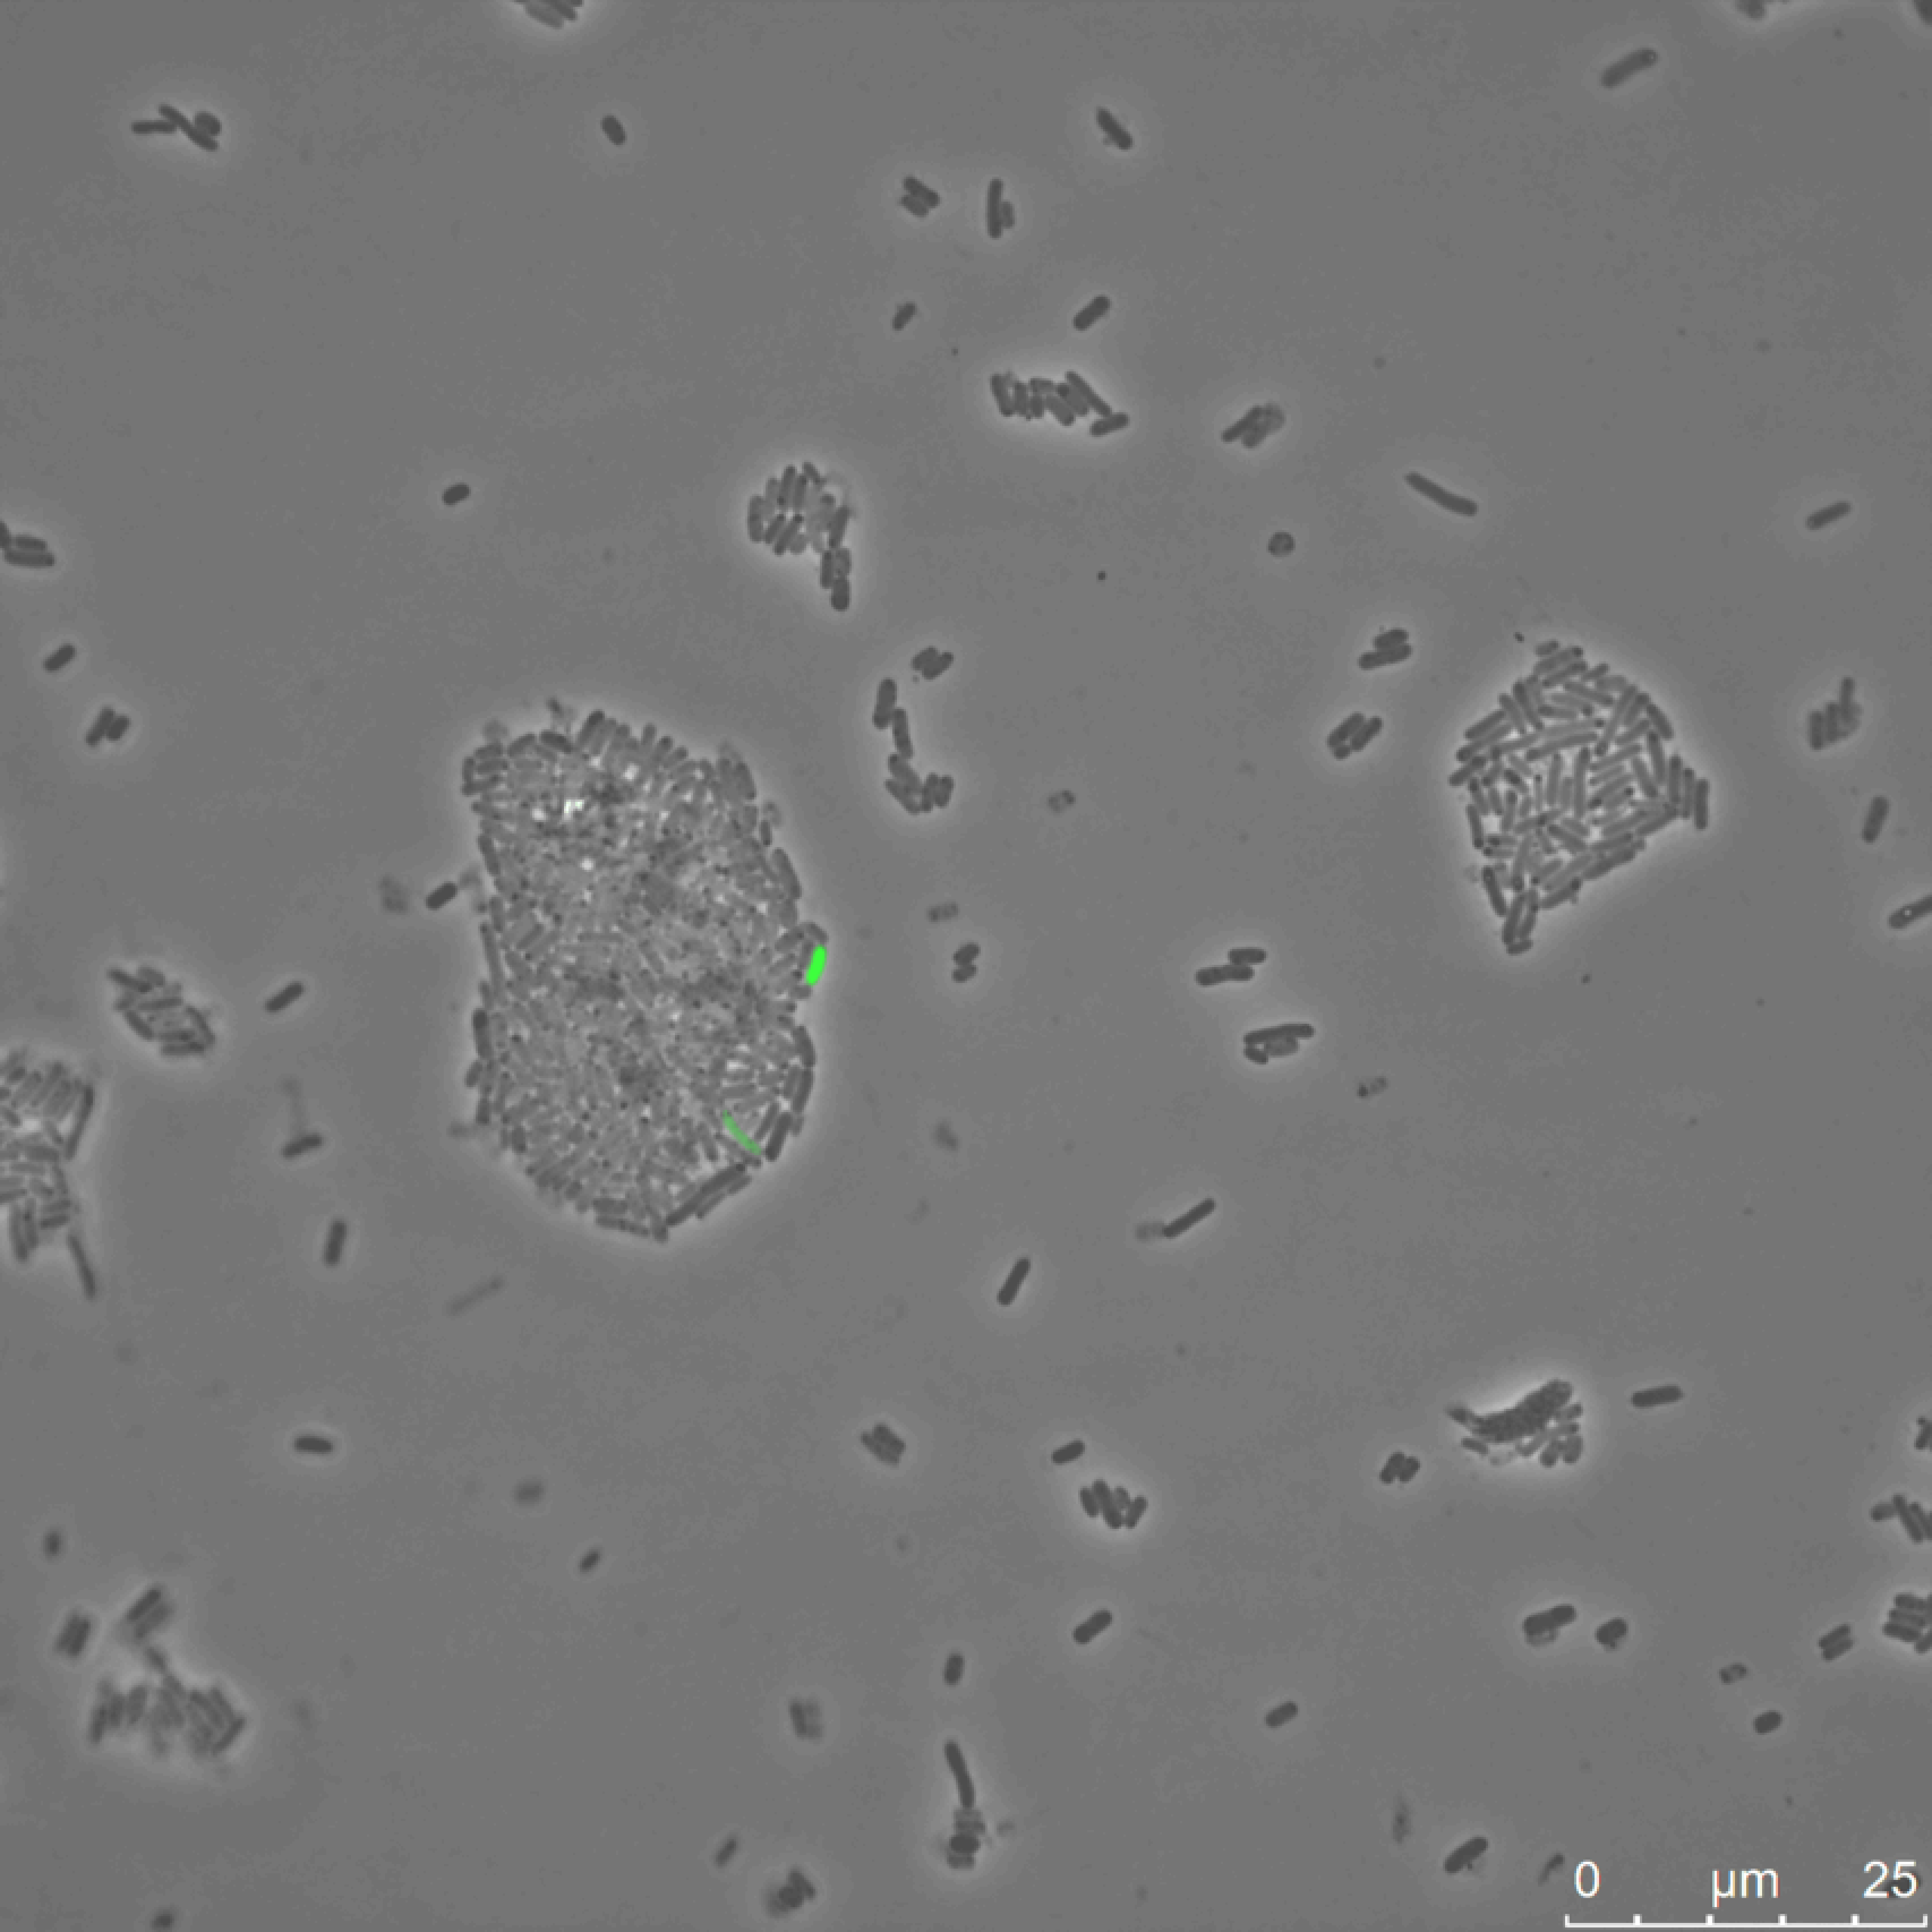
\includegraphics{THAIU1_72HR_1_GREEN-crunch-lighter-resample.pdf} \\[-0.5ex]

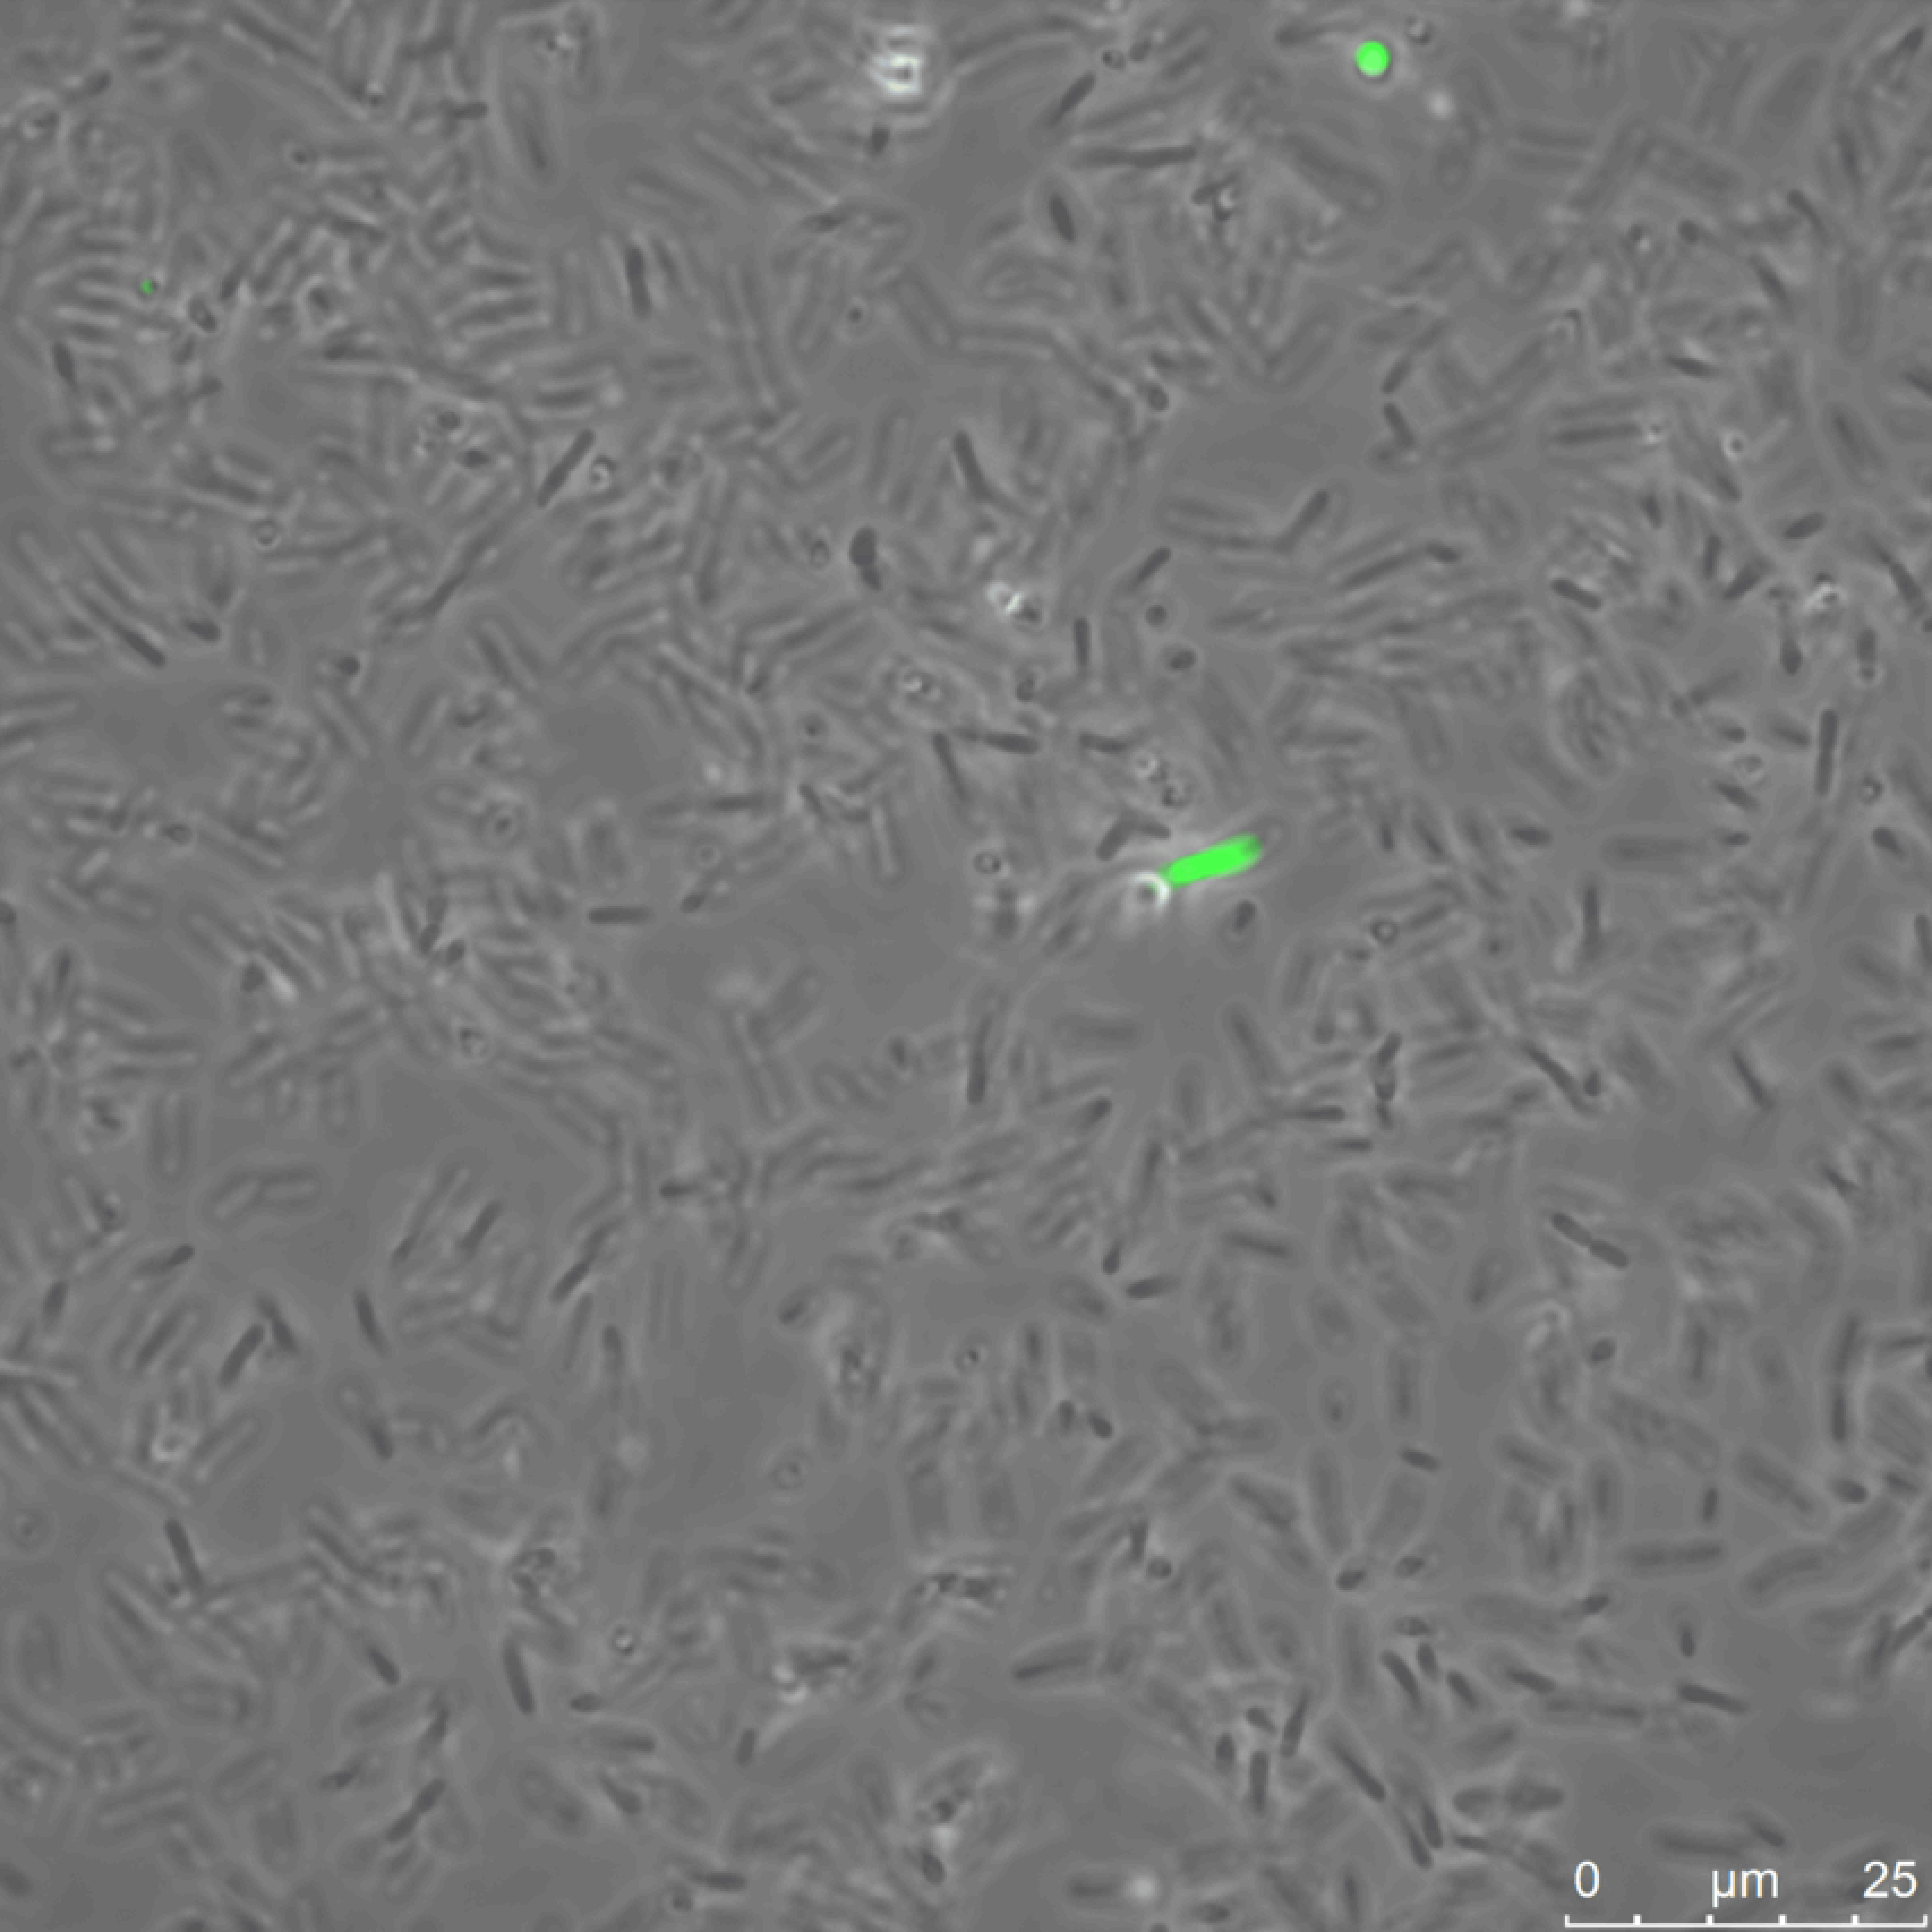
\includegraphics{THAIU1_2_GREEN-crunch-lighter-resample.pdf} &%
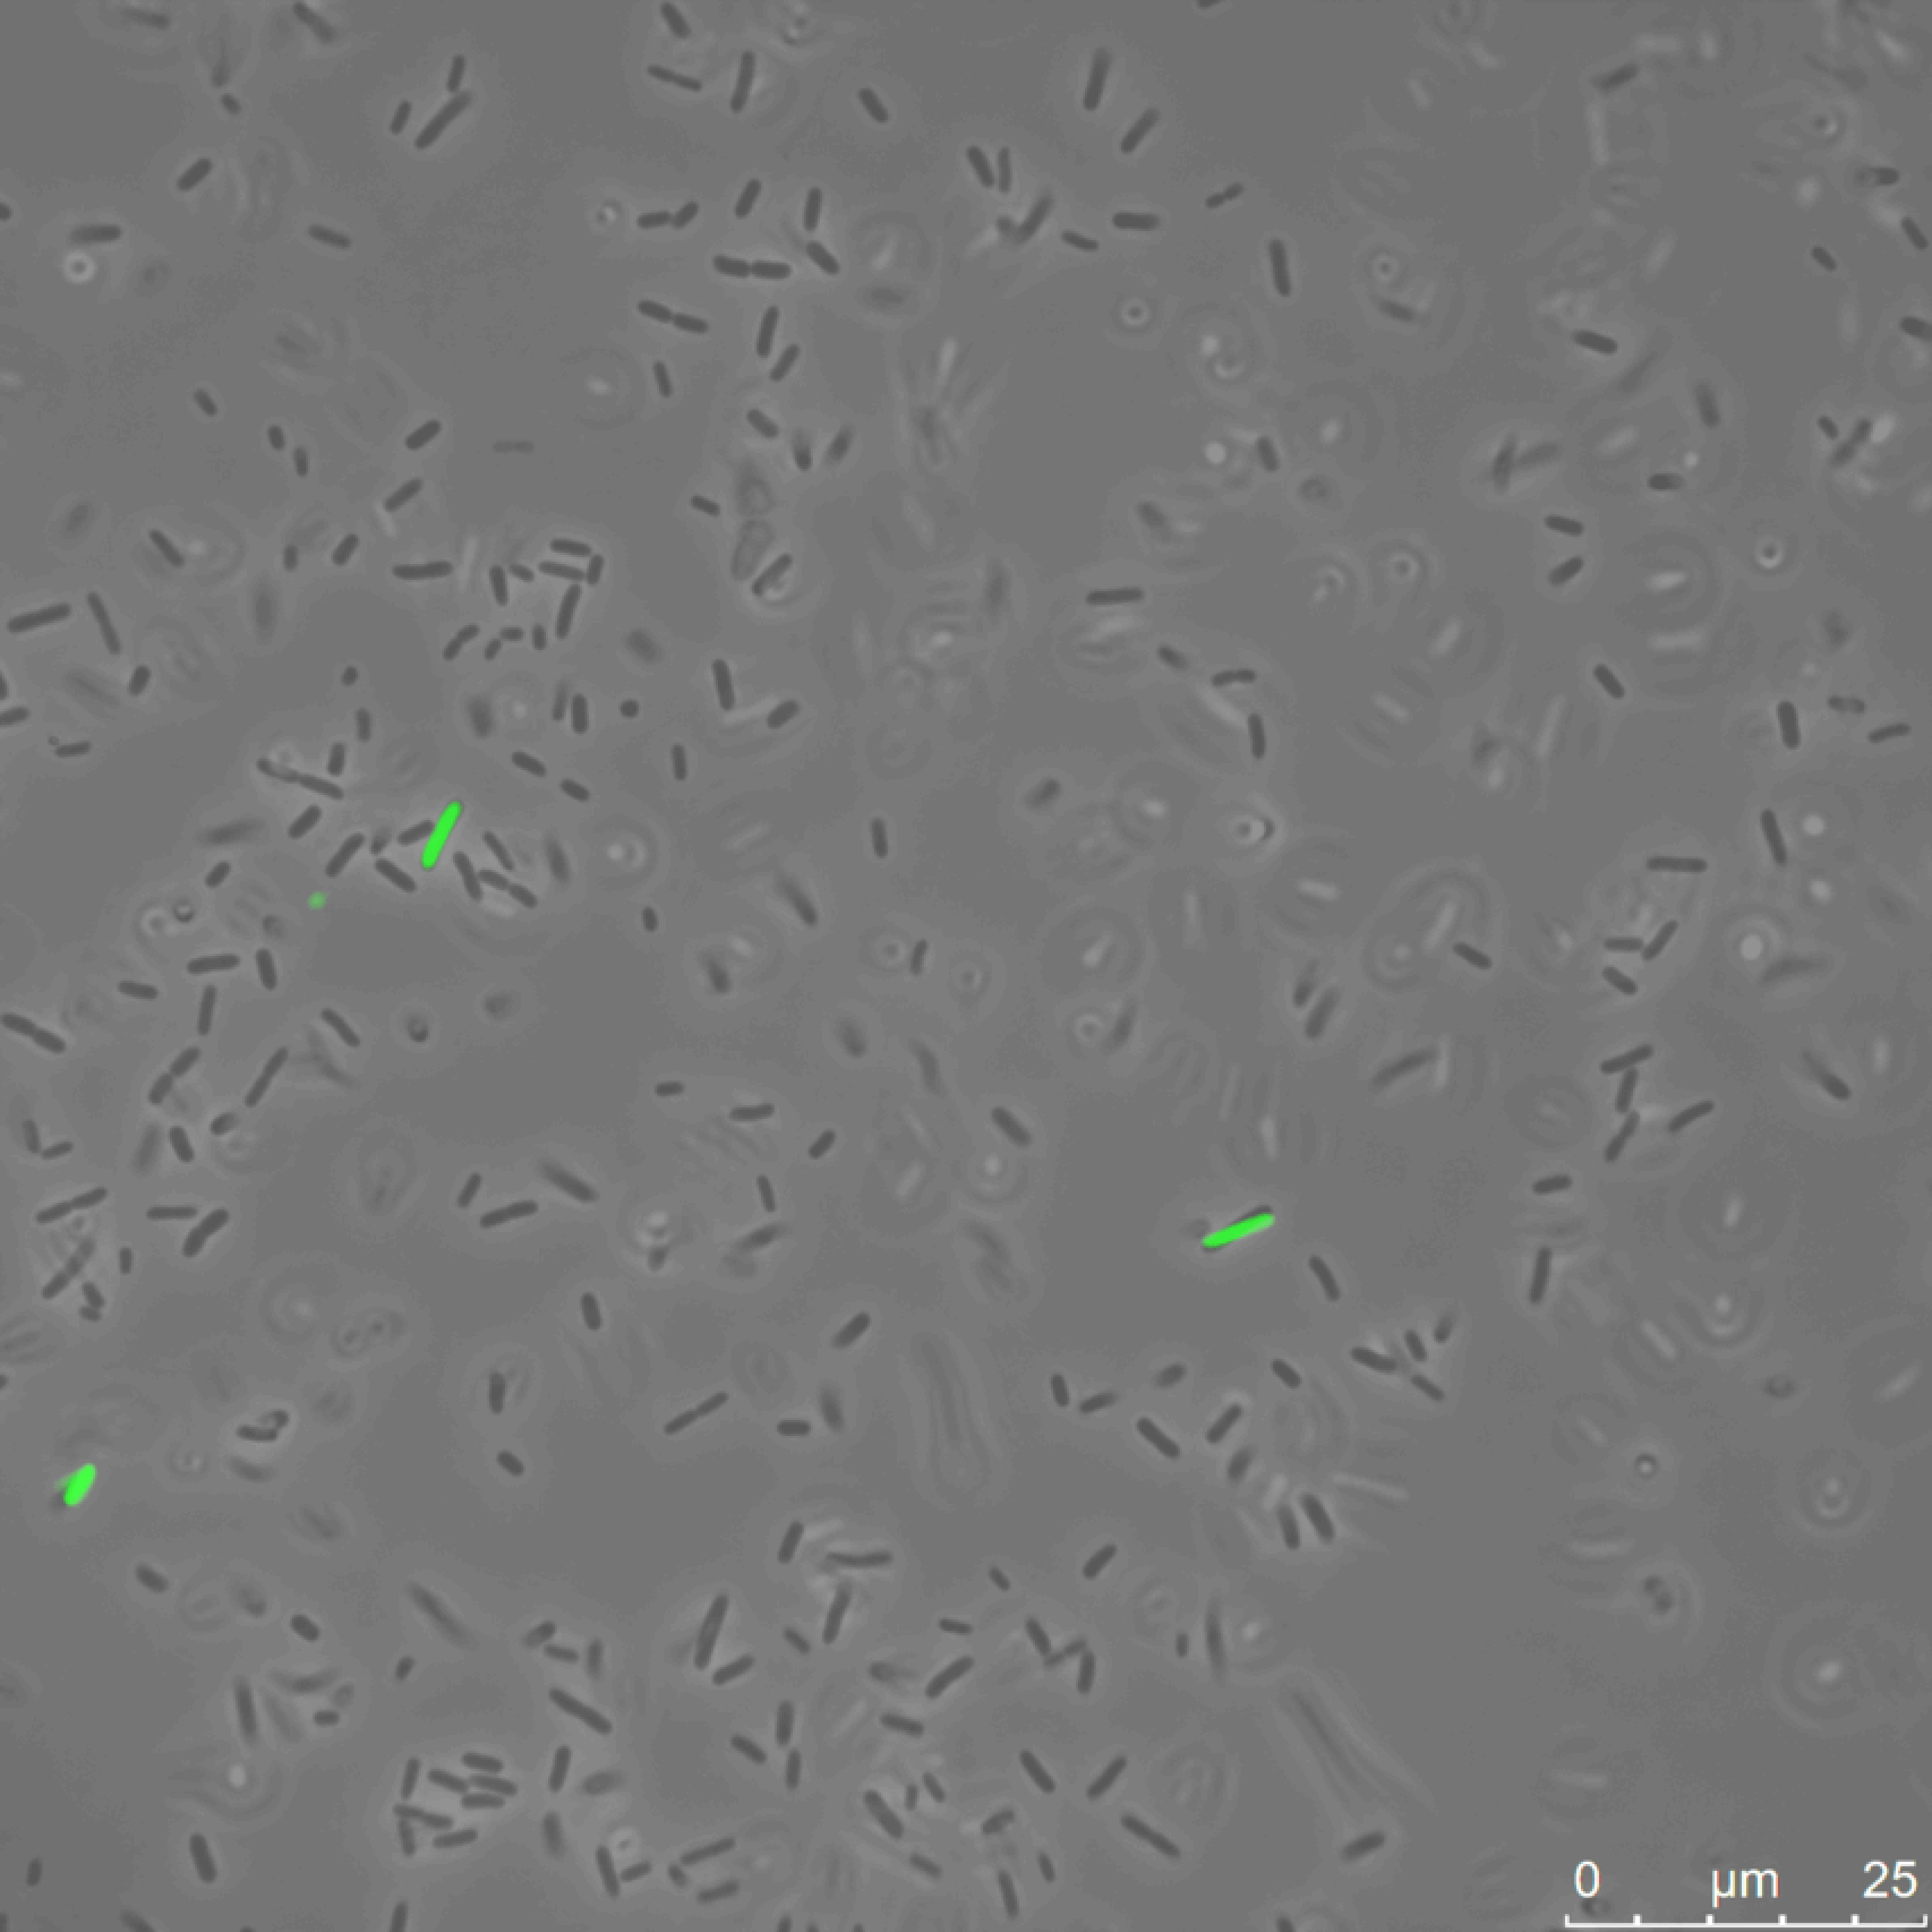
\includegraphics{THAIU1_5HR_5_GREEN-crunch-lighter-resample.pdf} &%
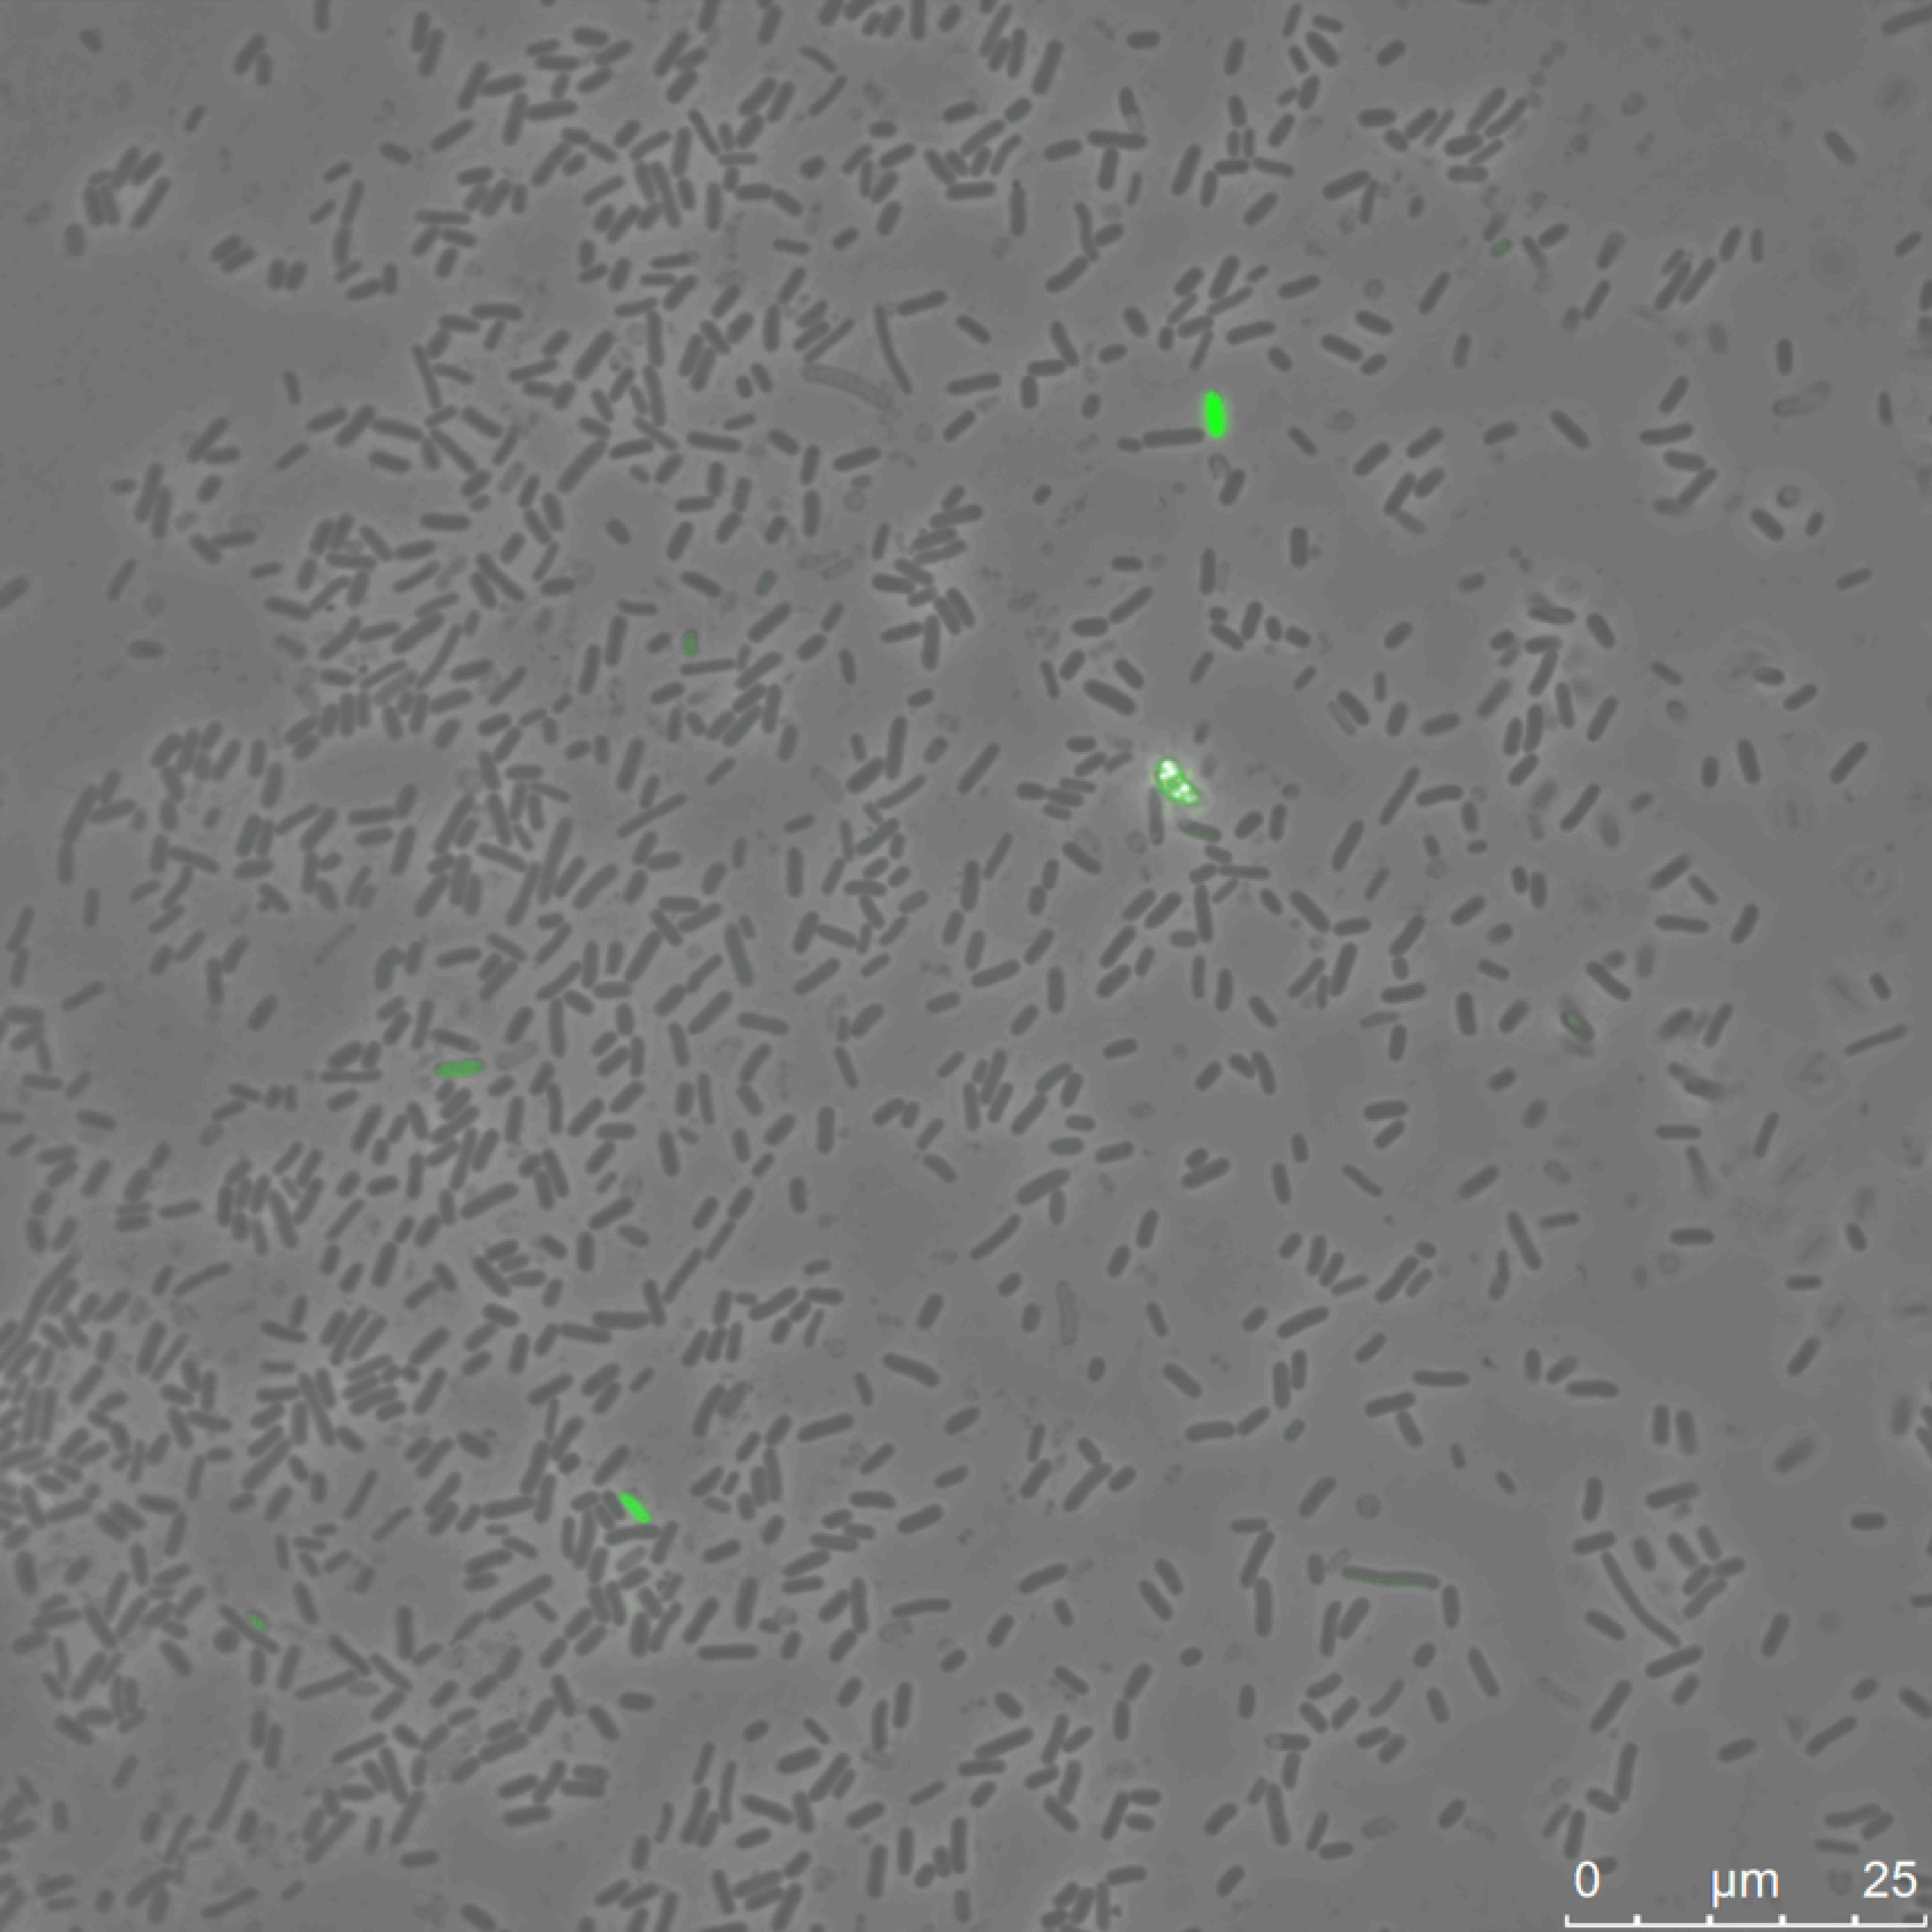
\includegraphics{THAIU1_24HR_2_GREEN-crunch-lighter-resample.pdf} &%
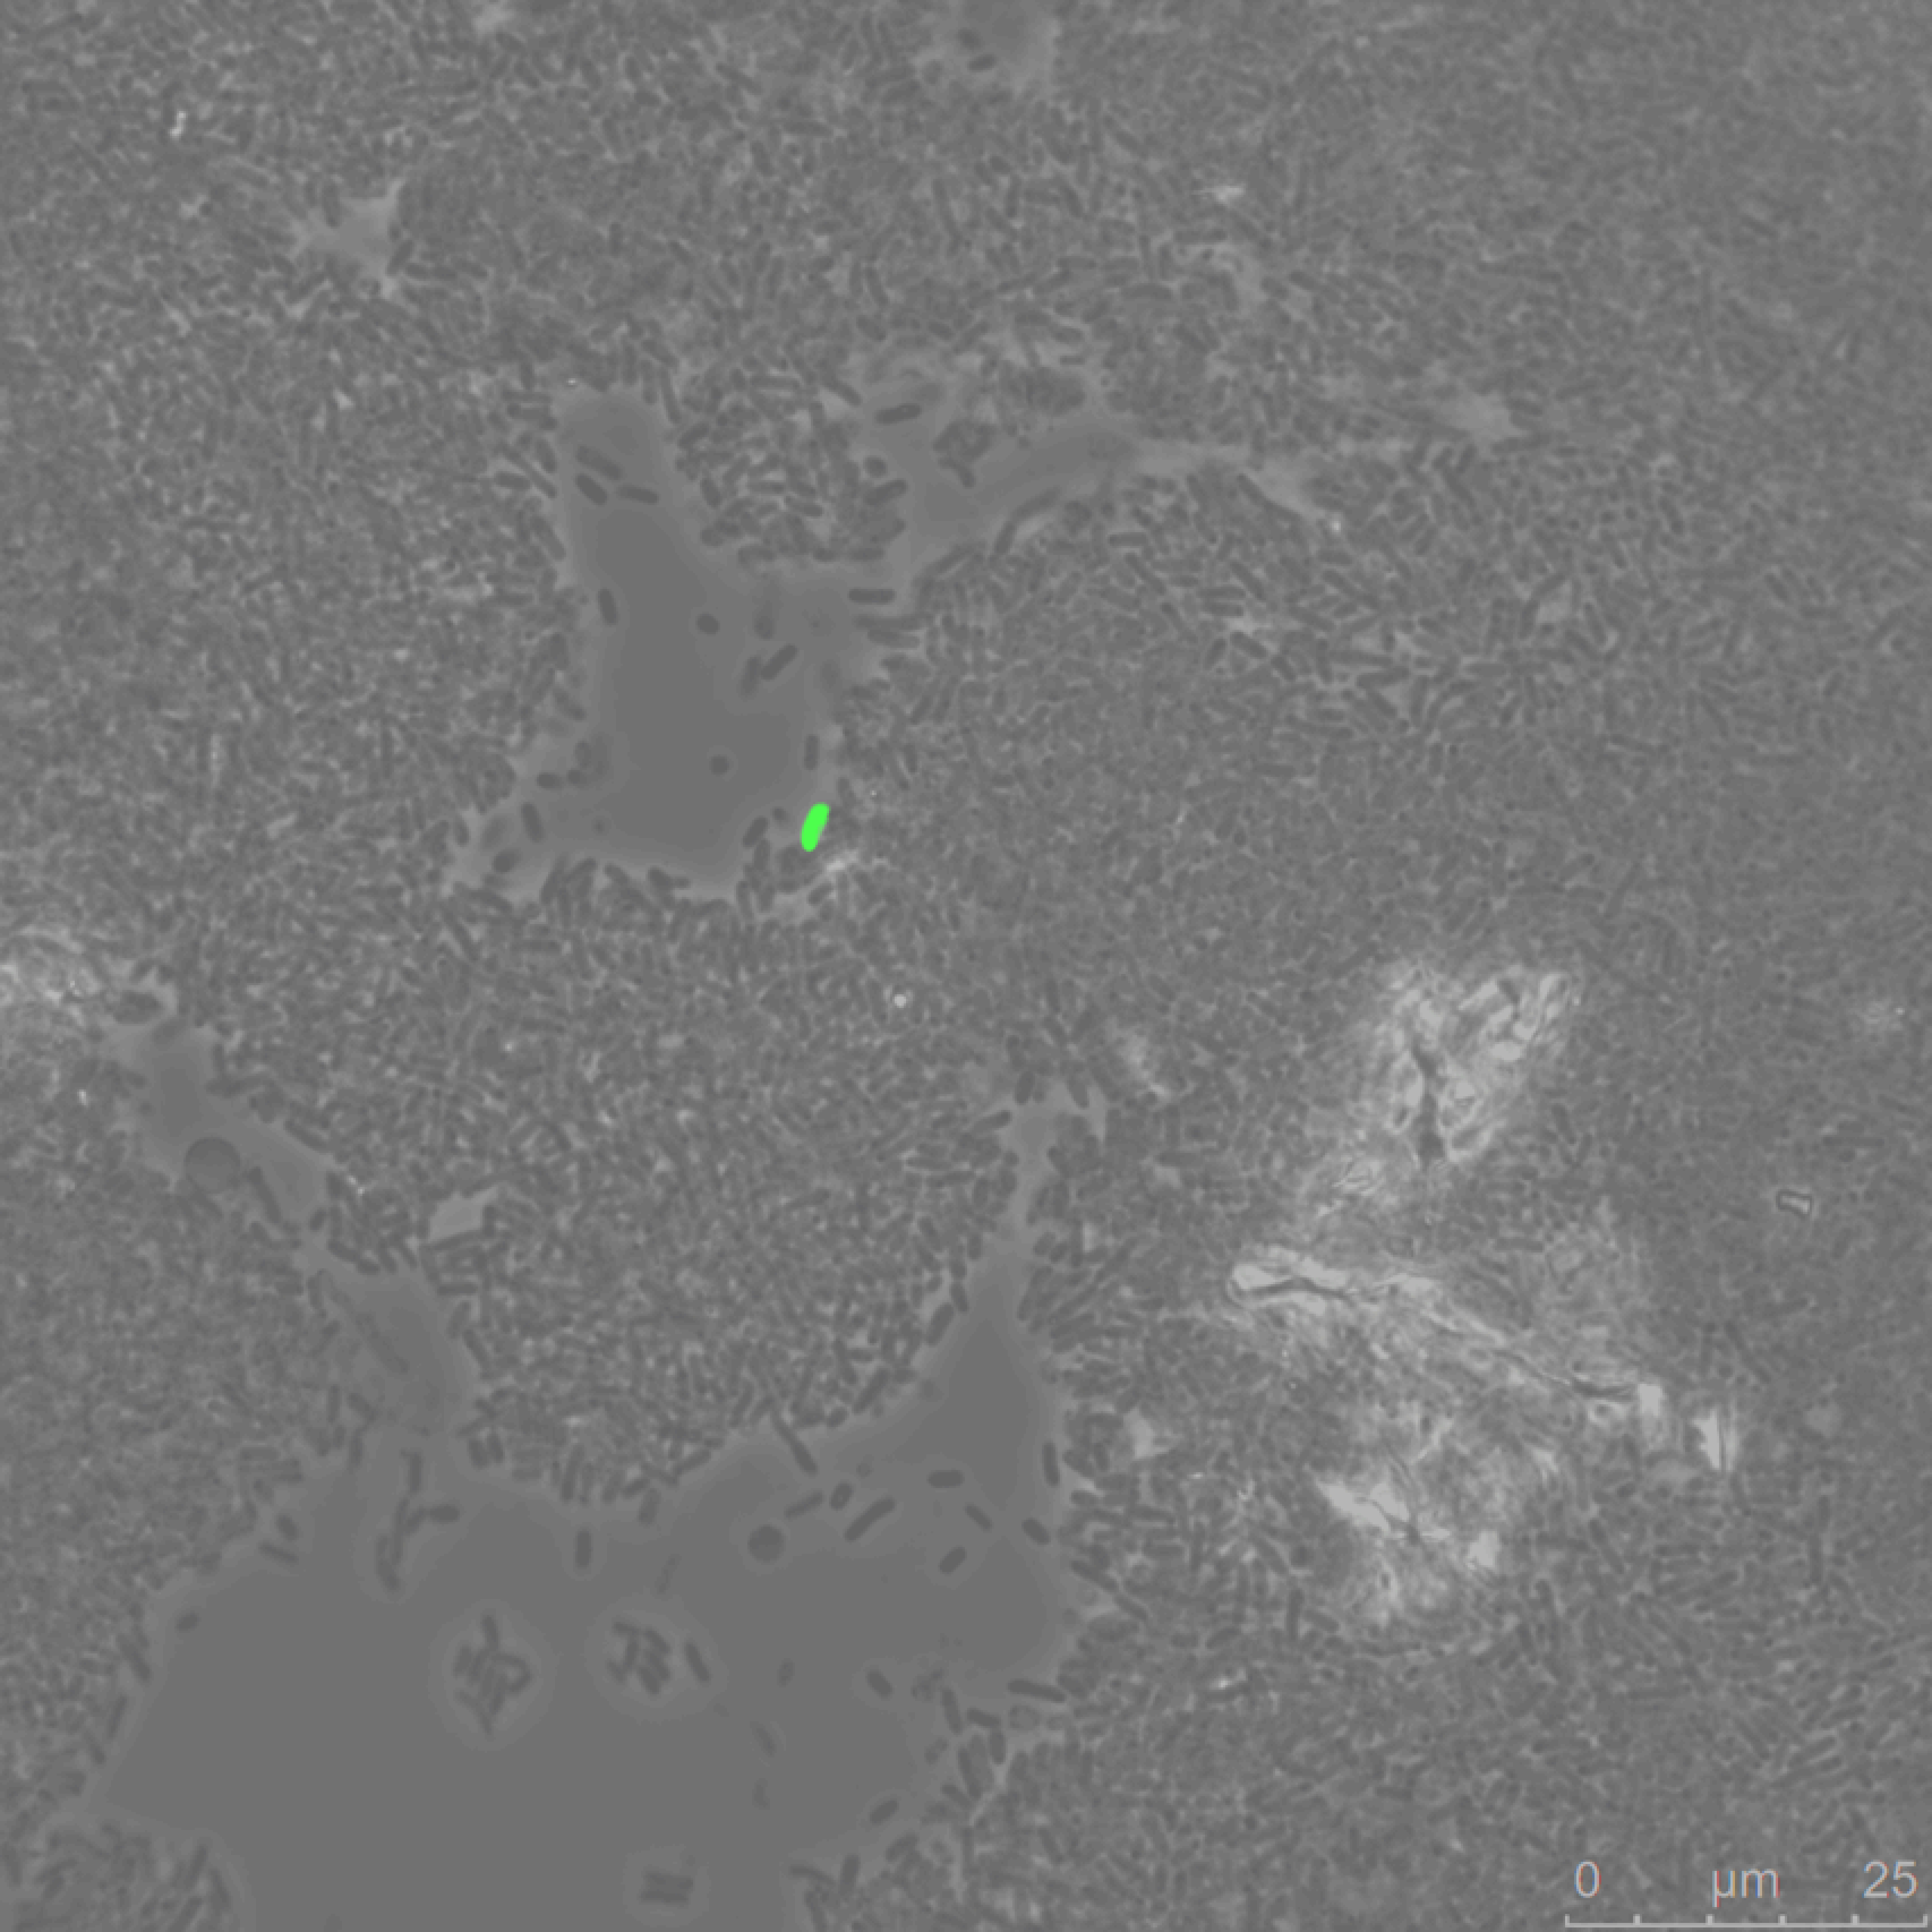
\includegraphics{THAIU1_72HR_2_GREEN-crunch-lighter-resample.pdf} \\[-0.5ex]

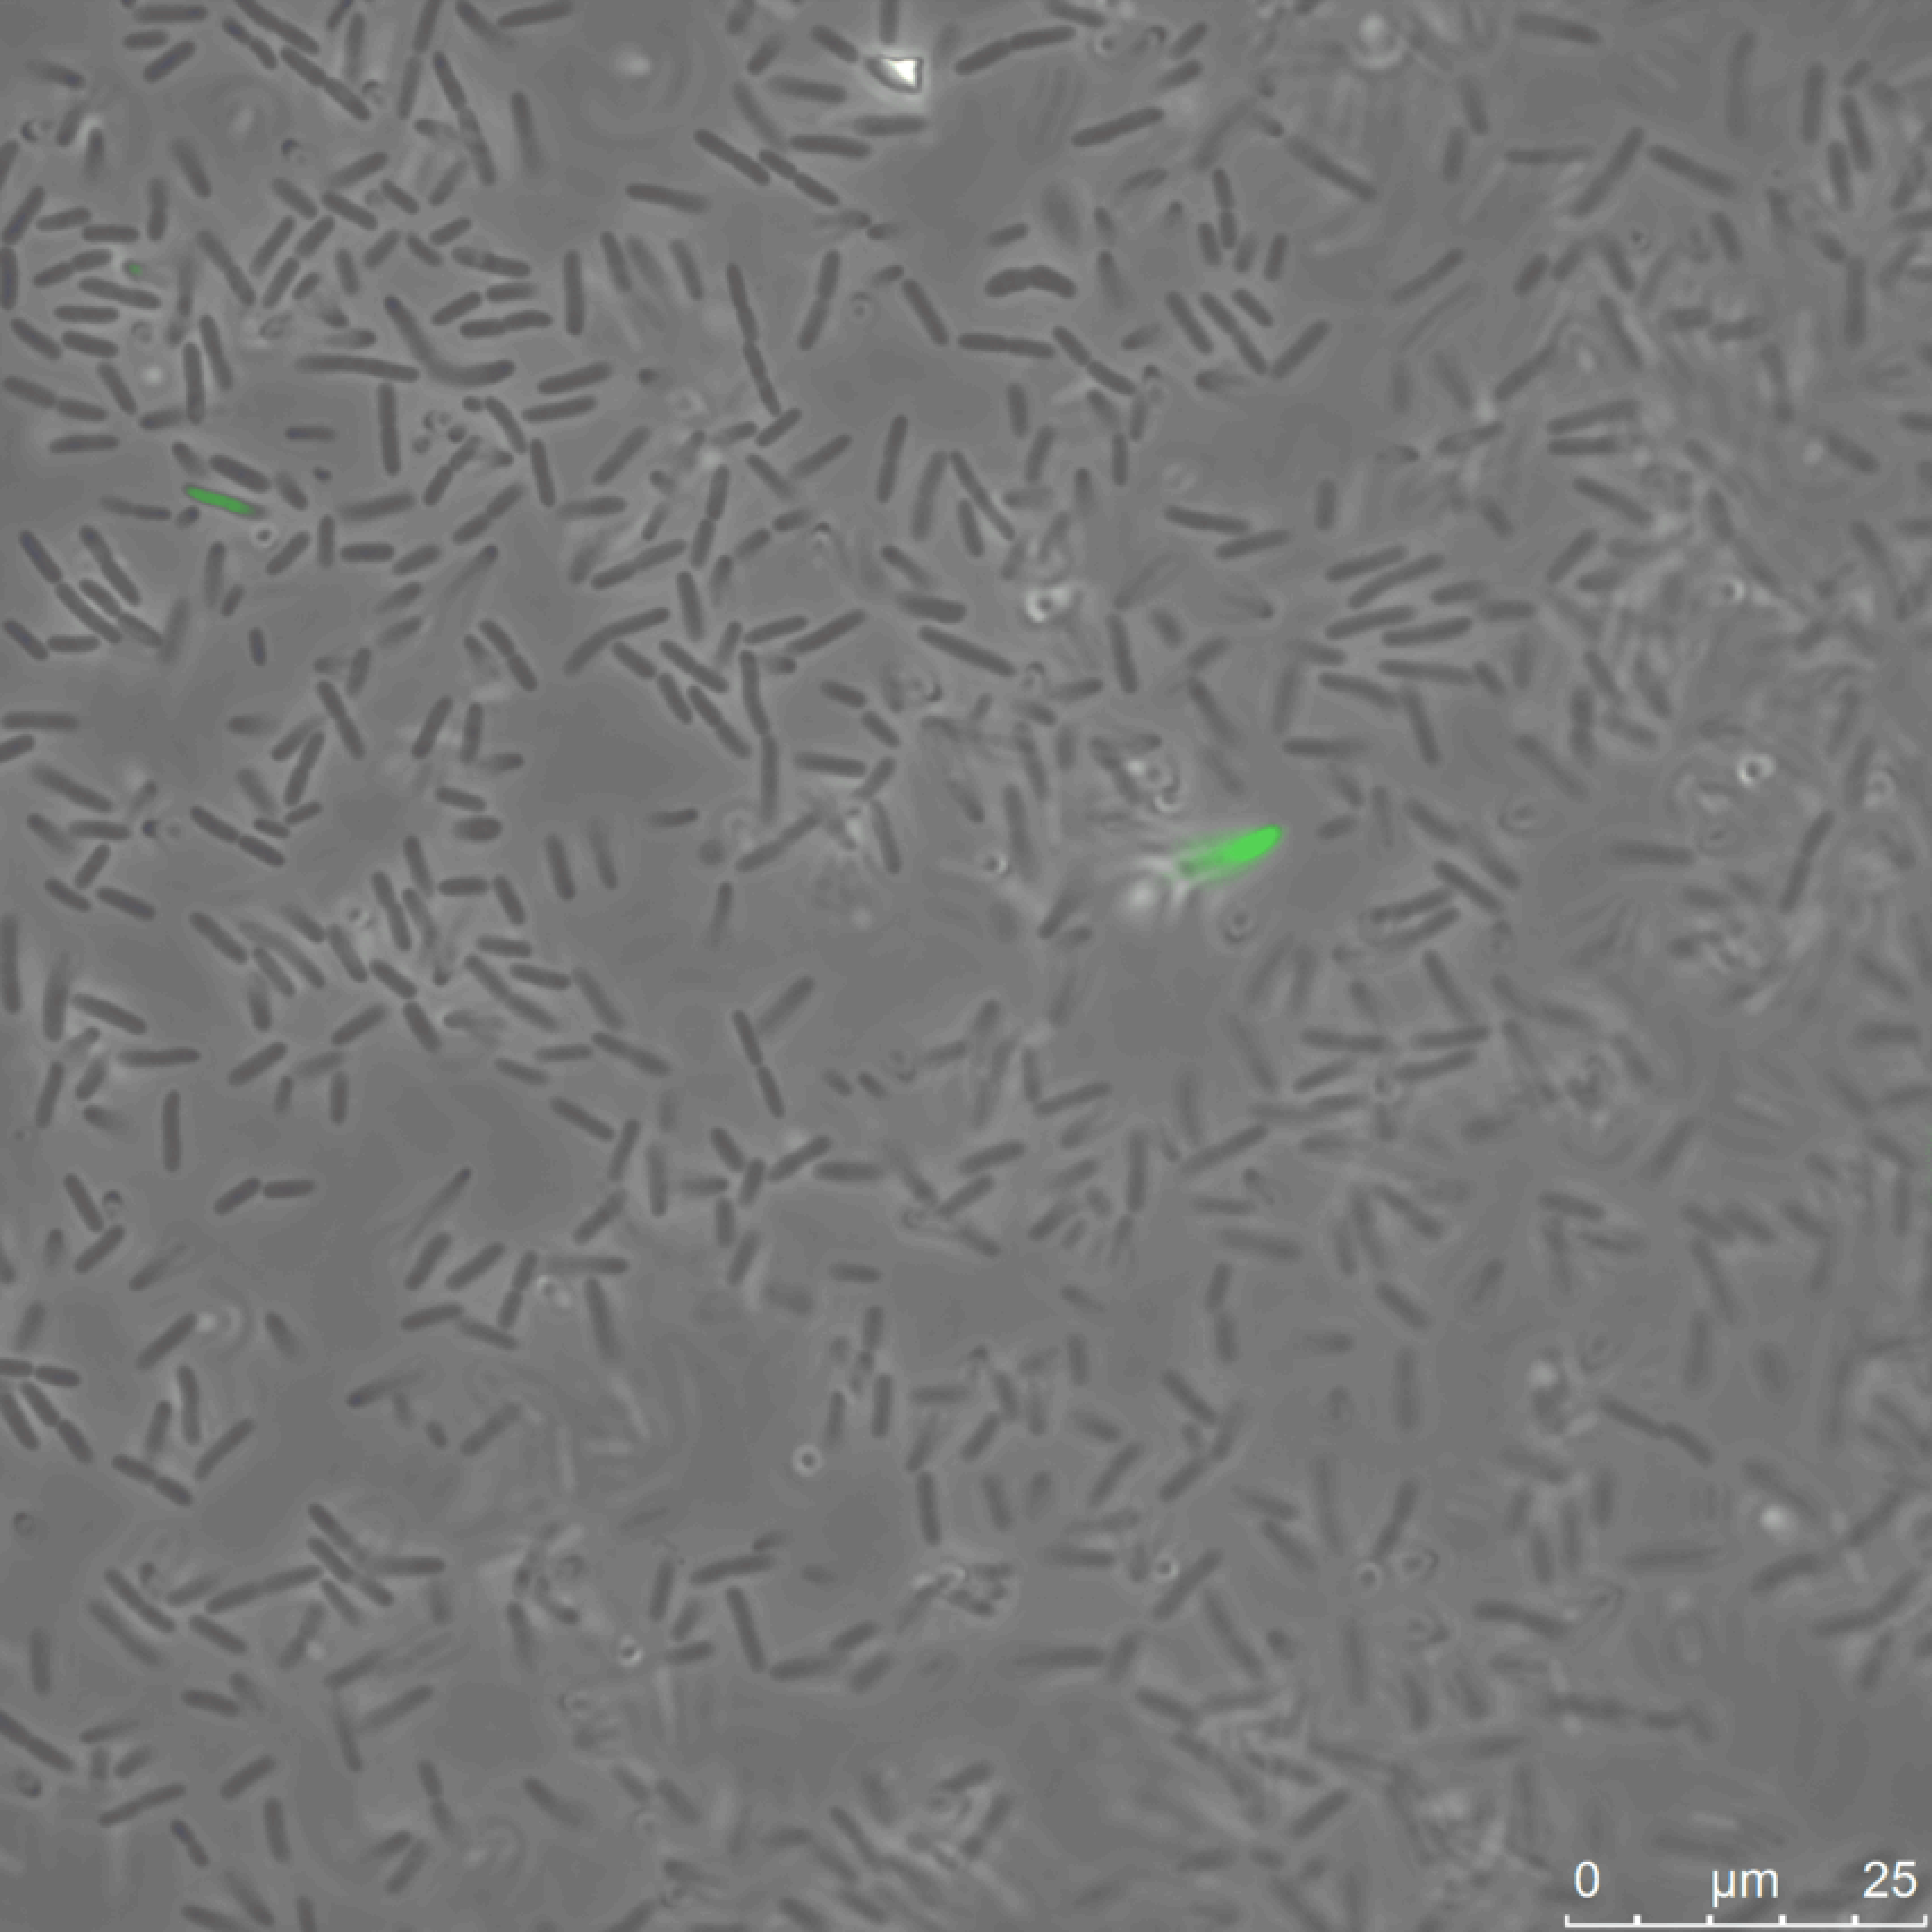
\includegraphics{THAIU1_3_GREEN-crunch-lighter-resample.pdf} &%
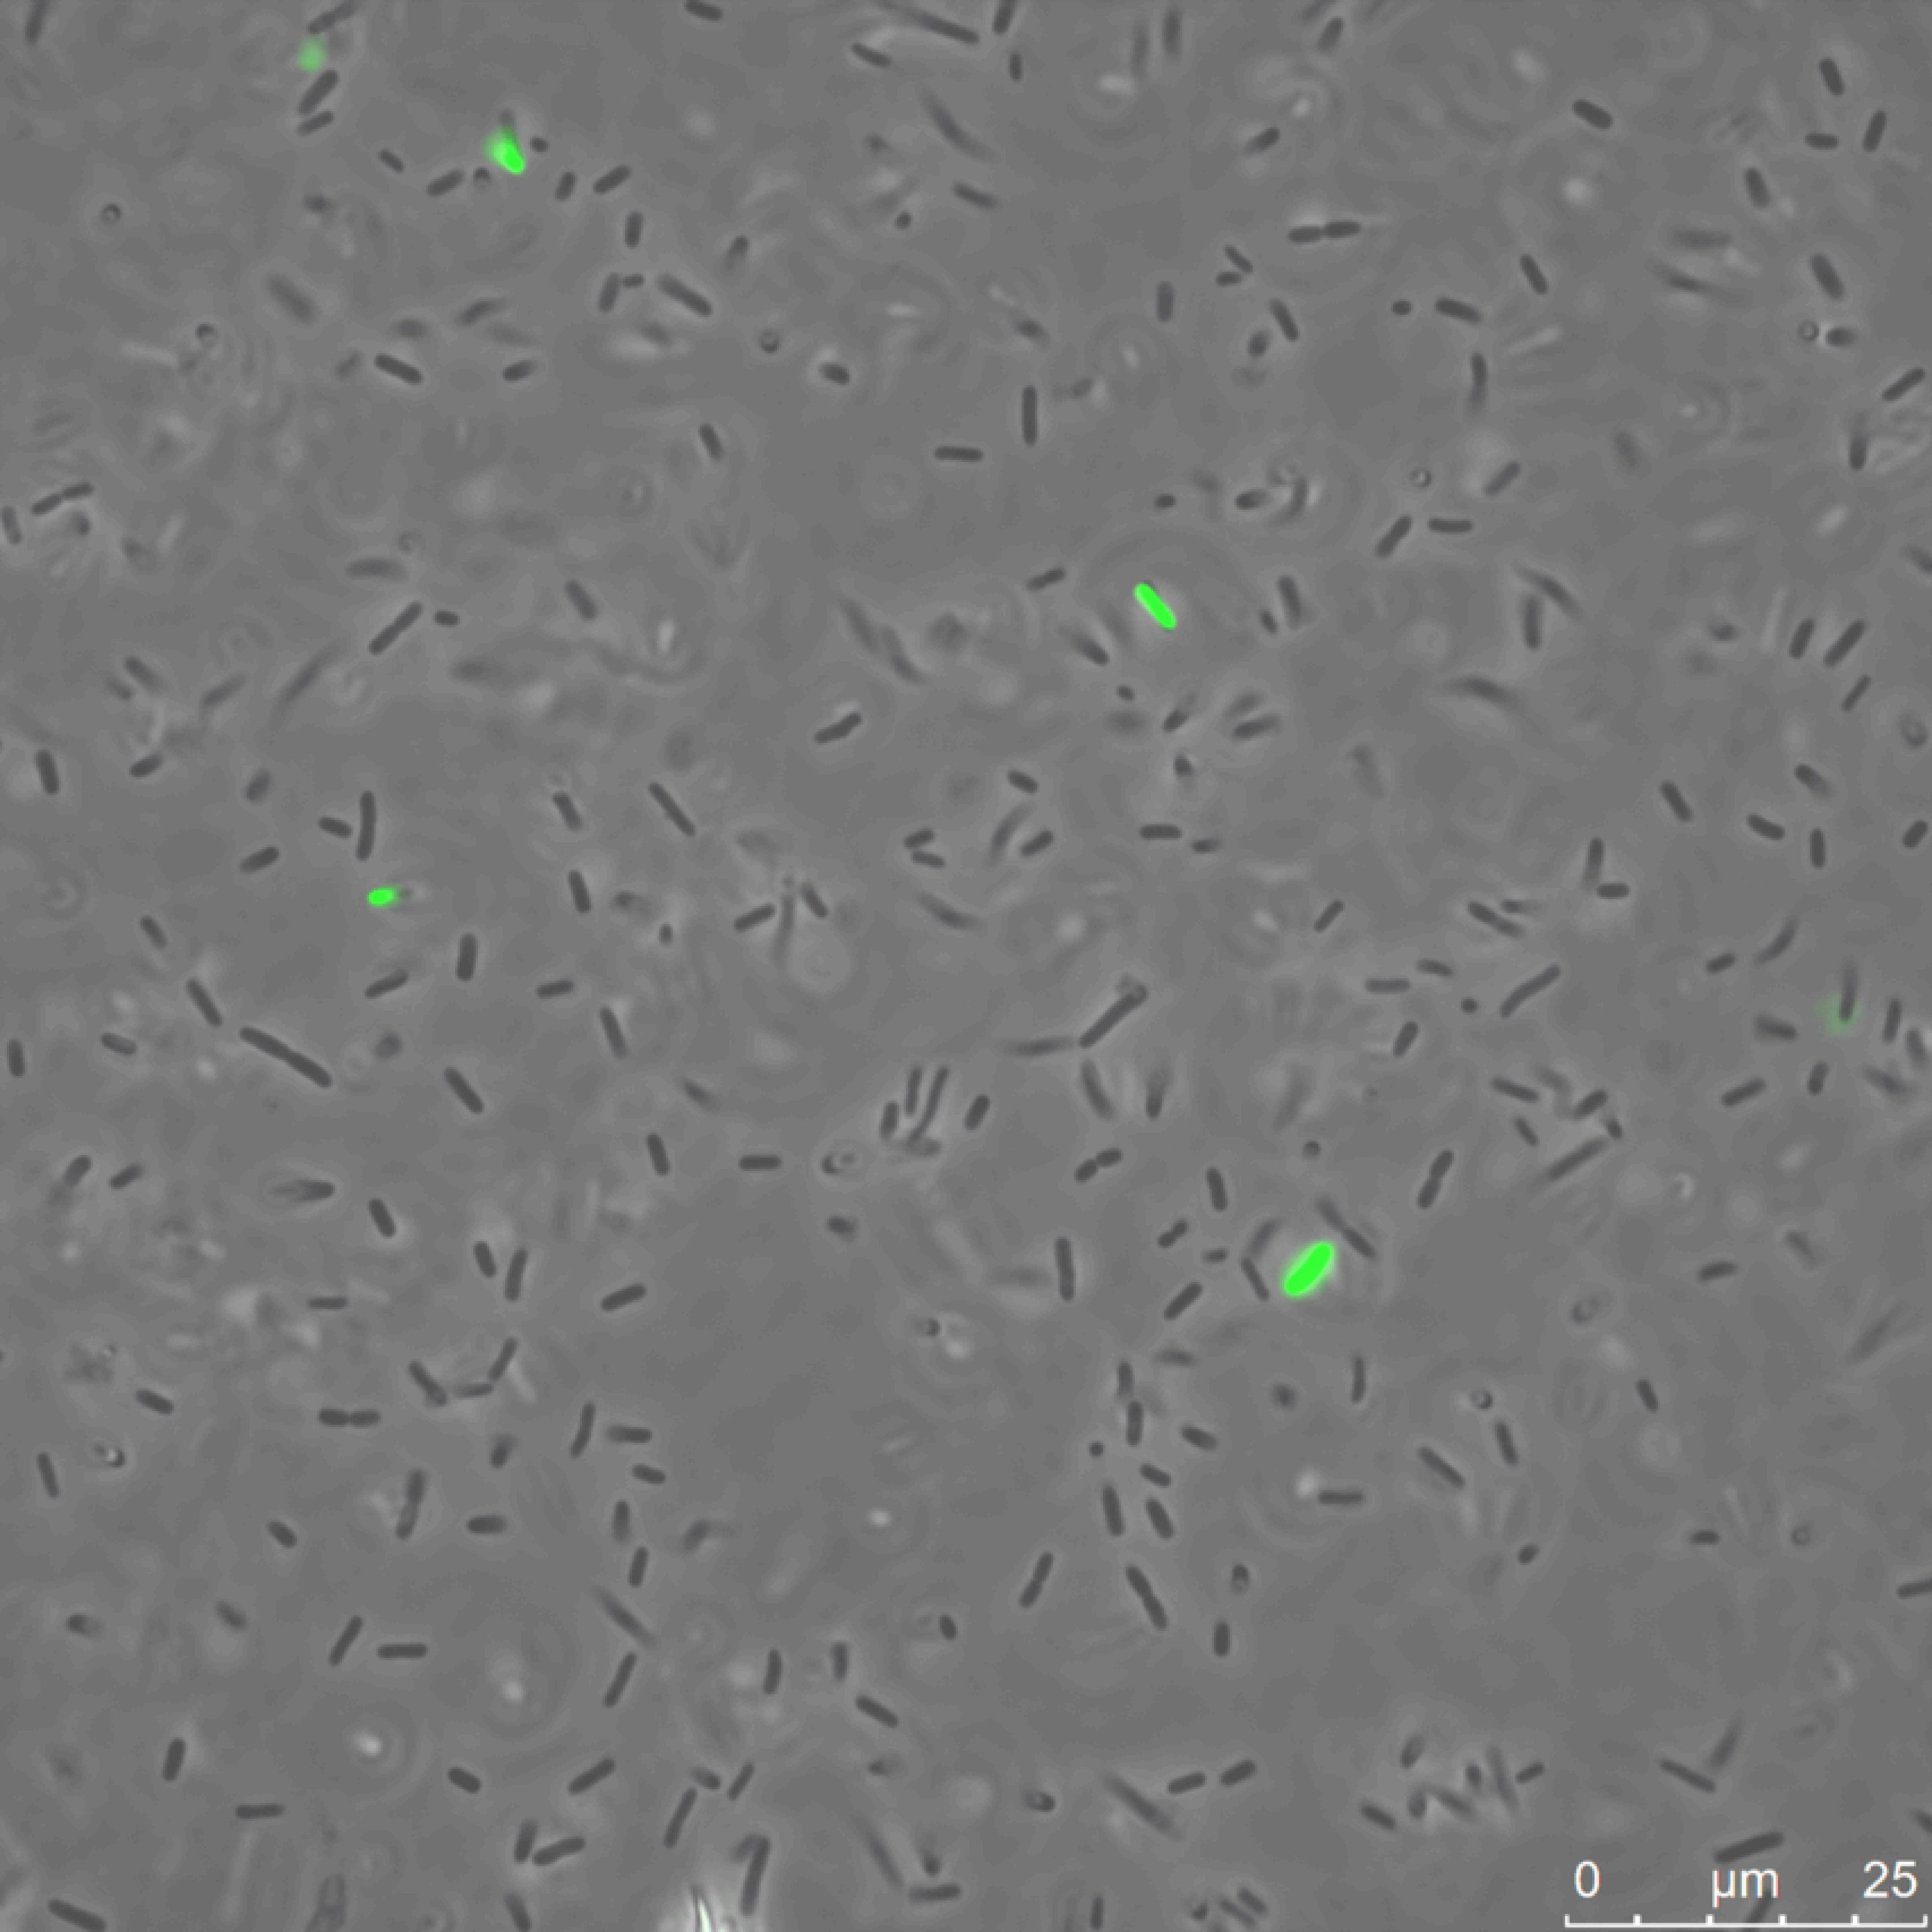
\includegraphics{THAIU1_5HR_3_GREEN-crunch-lighter-resample.pdf} &%
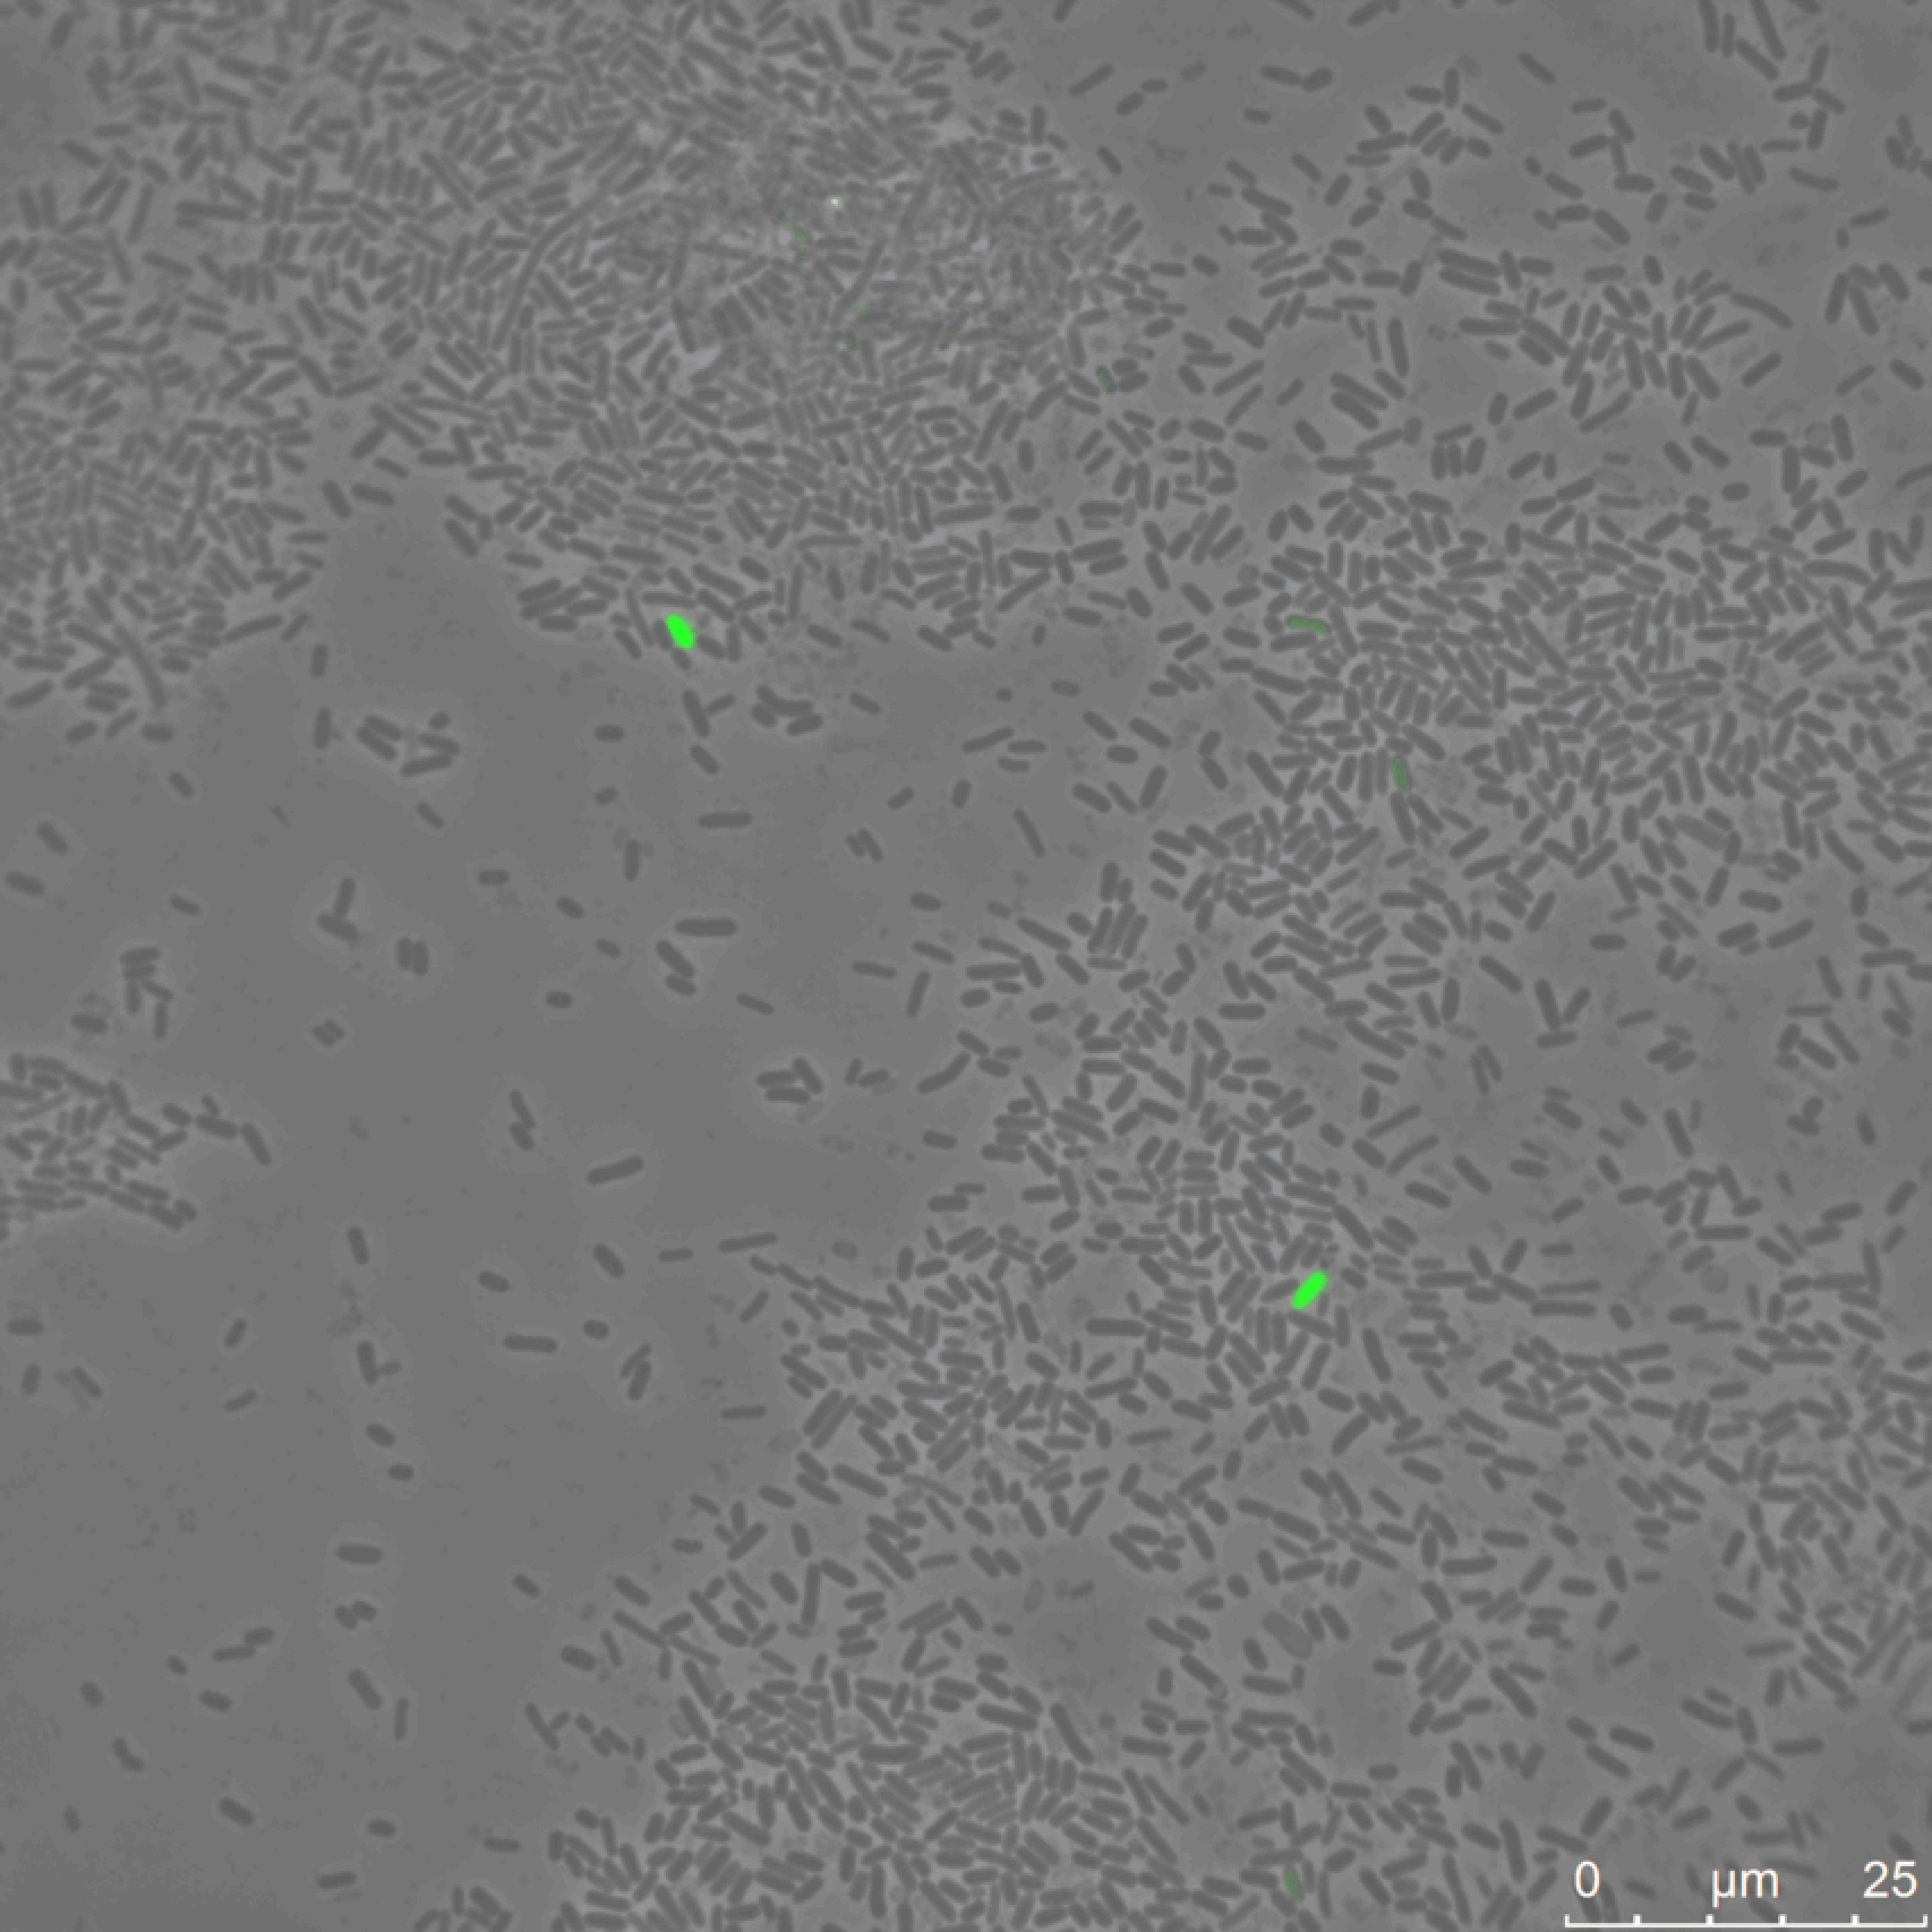
\includegraphics{THAIU1_24HR_6_GREEN-crunch-lighter-resample.pdf} &%
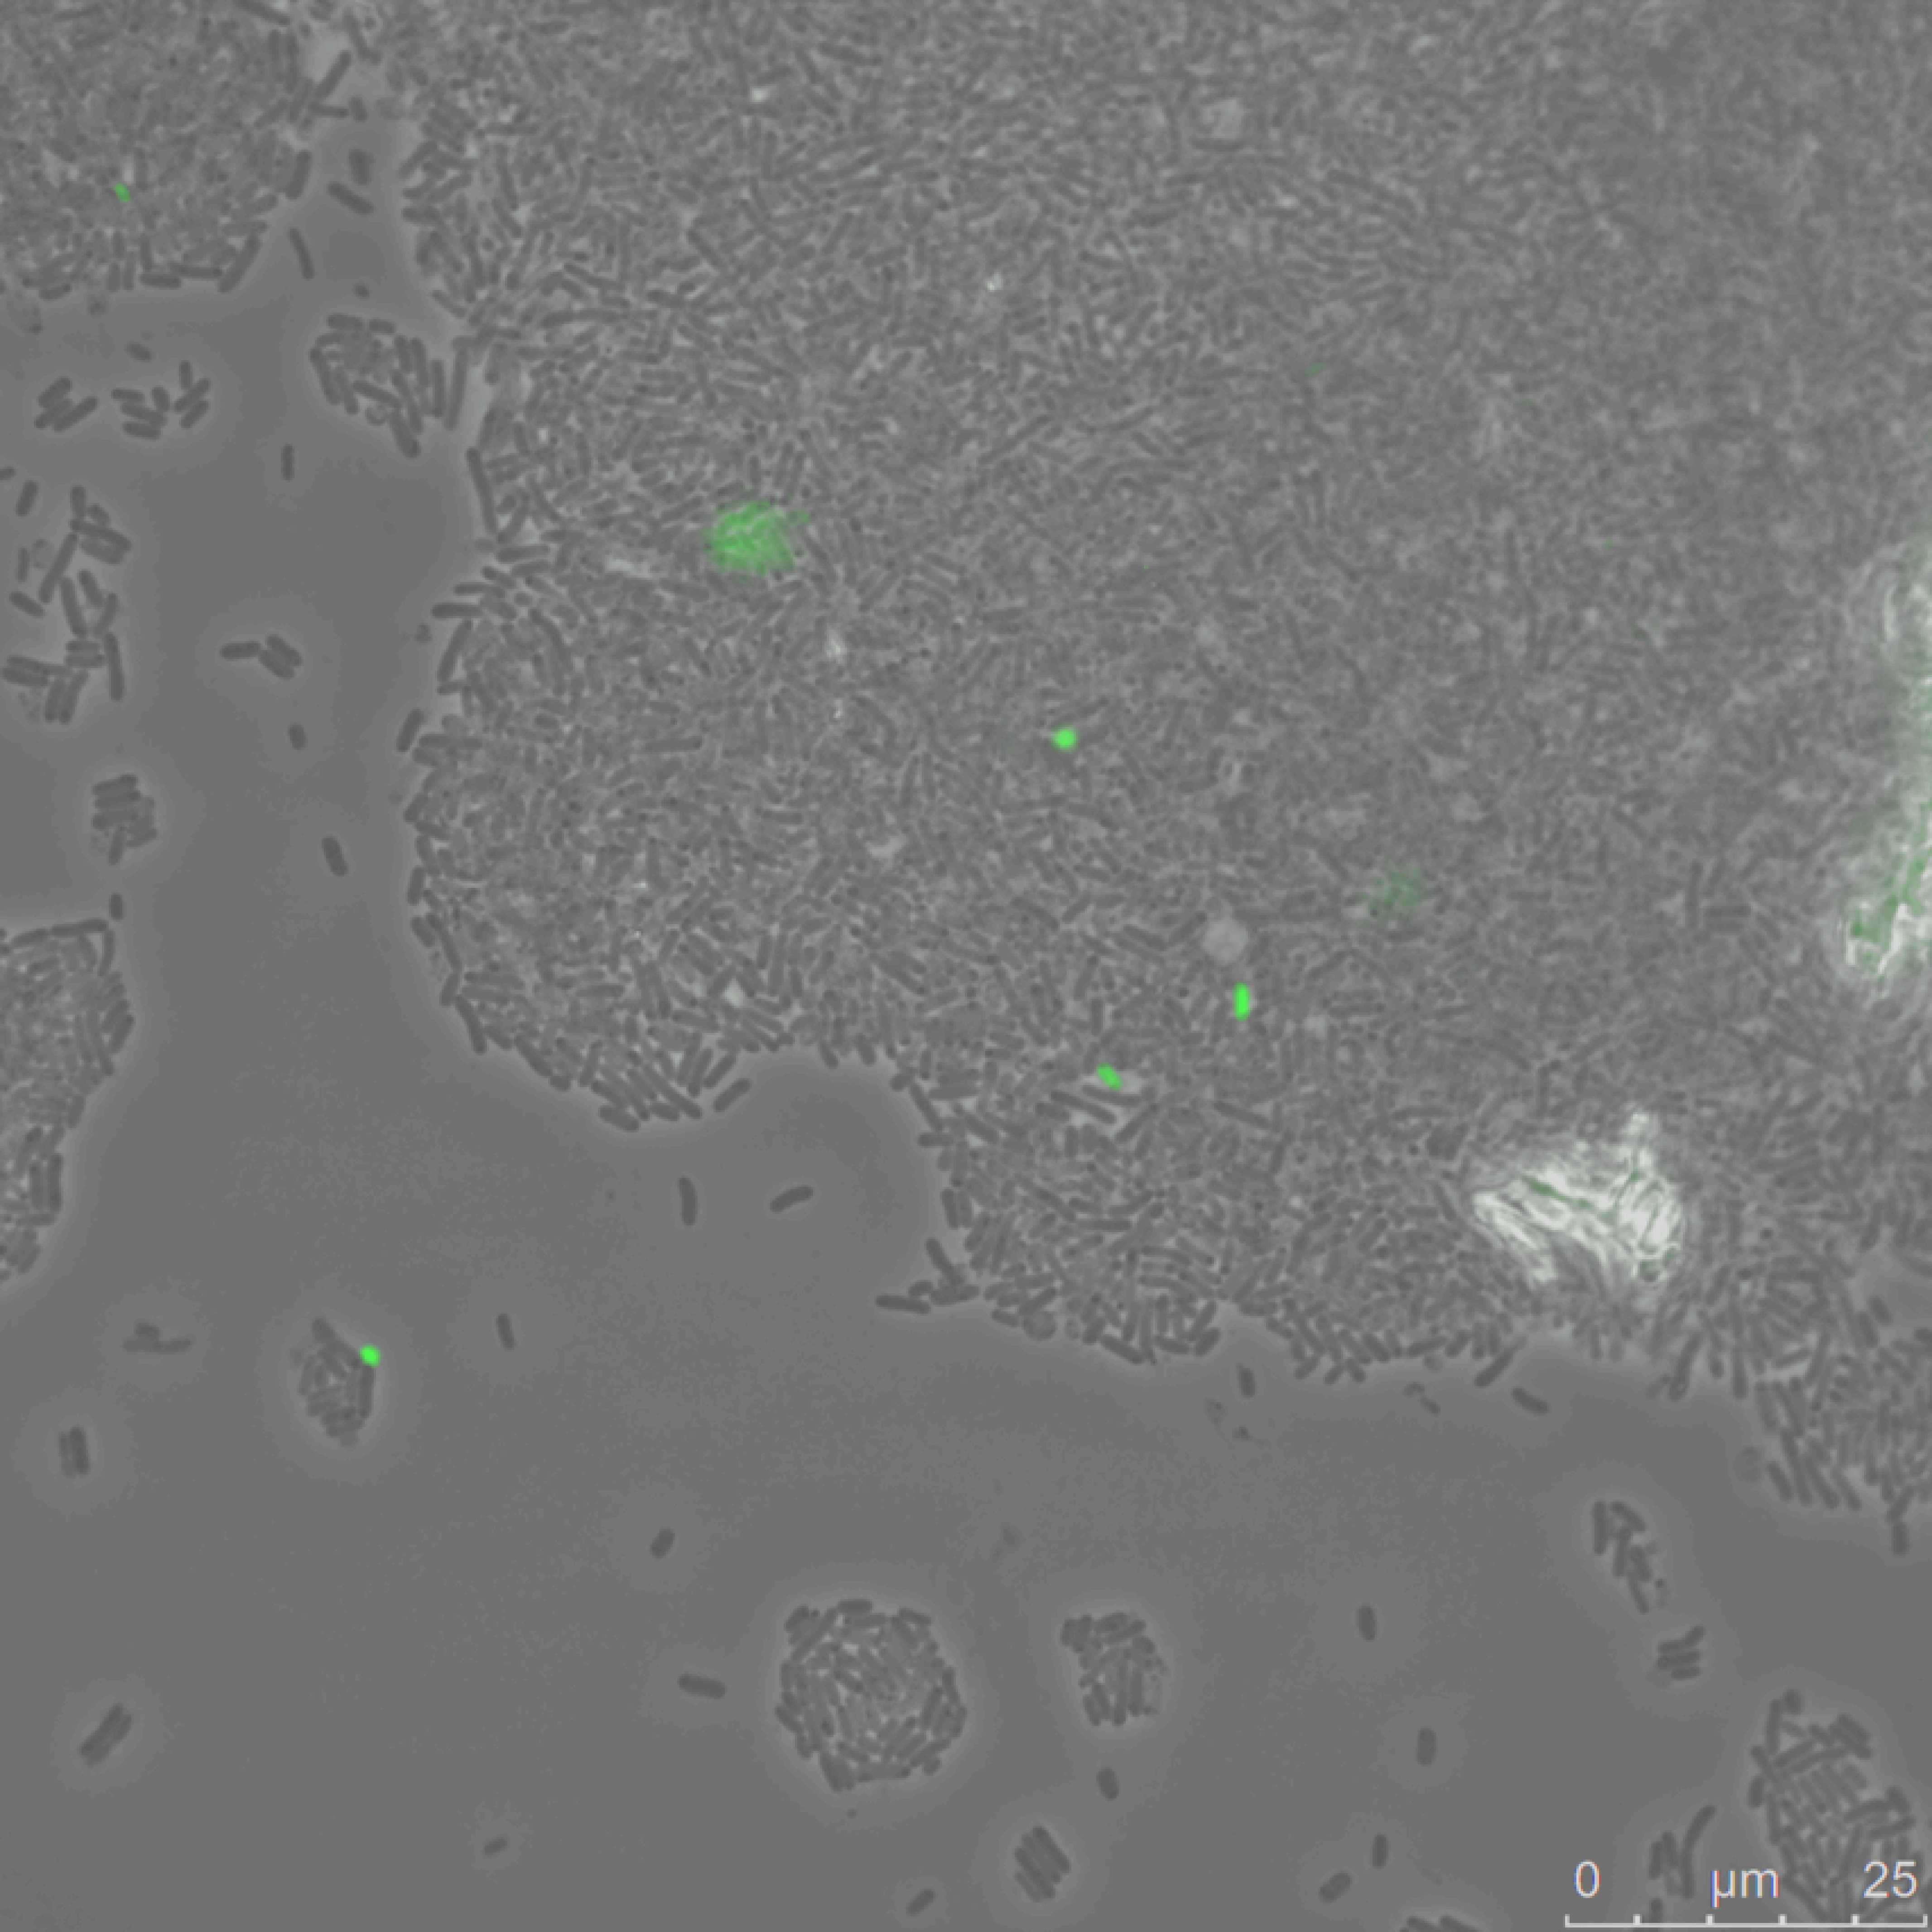
\includegraphics{THAIU1_72HR_3_GREEN-crunch-lighter-resample.pdf} \\[-0.5ex]

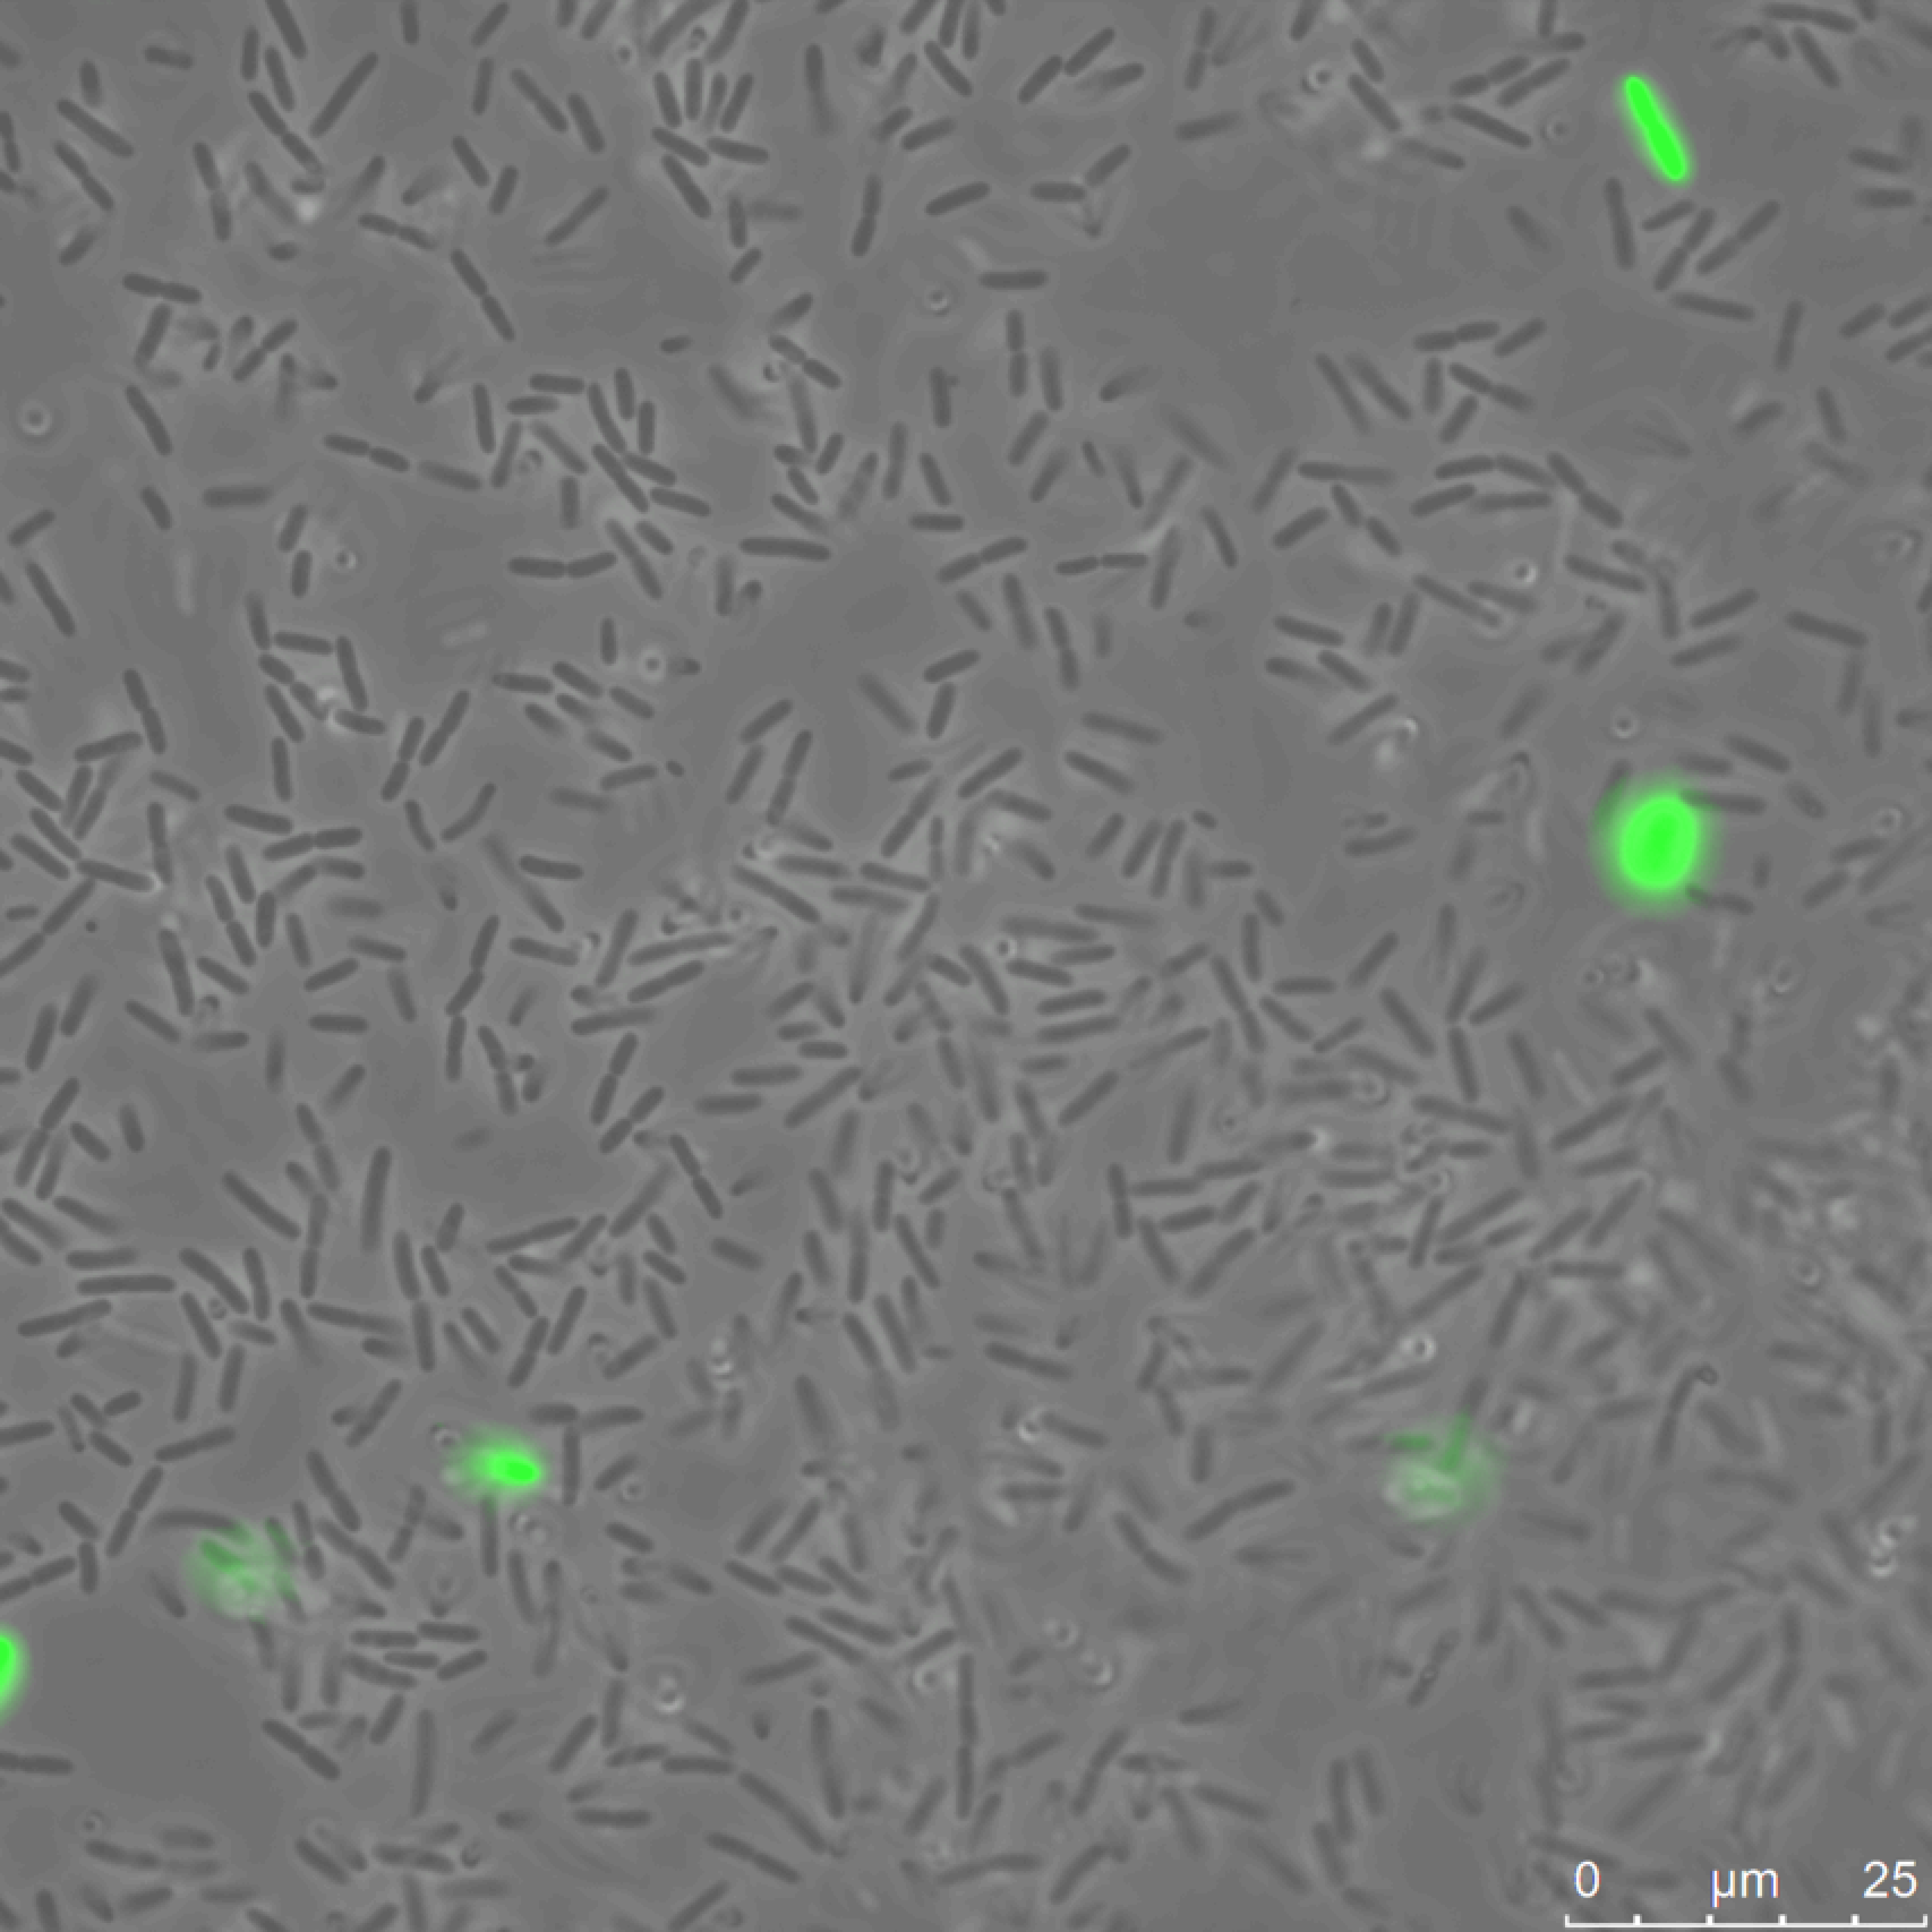
\includegraphics{THAIU1_4_GREEN-crunch-lighter-resample.pdf} &%
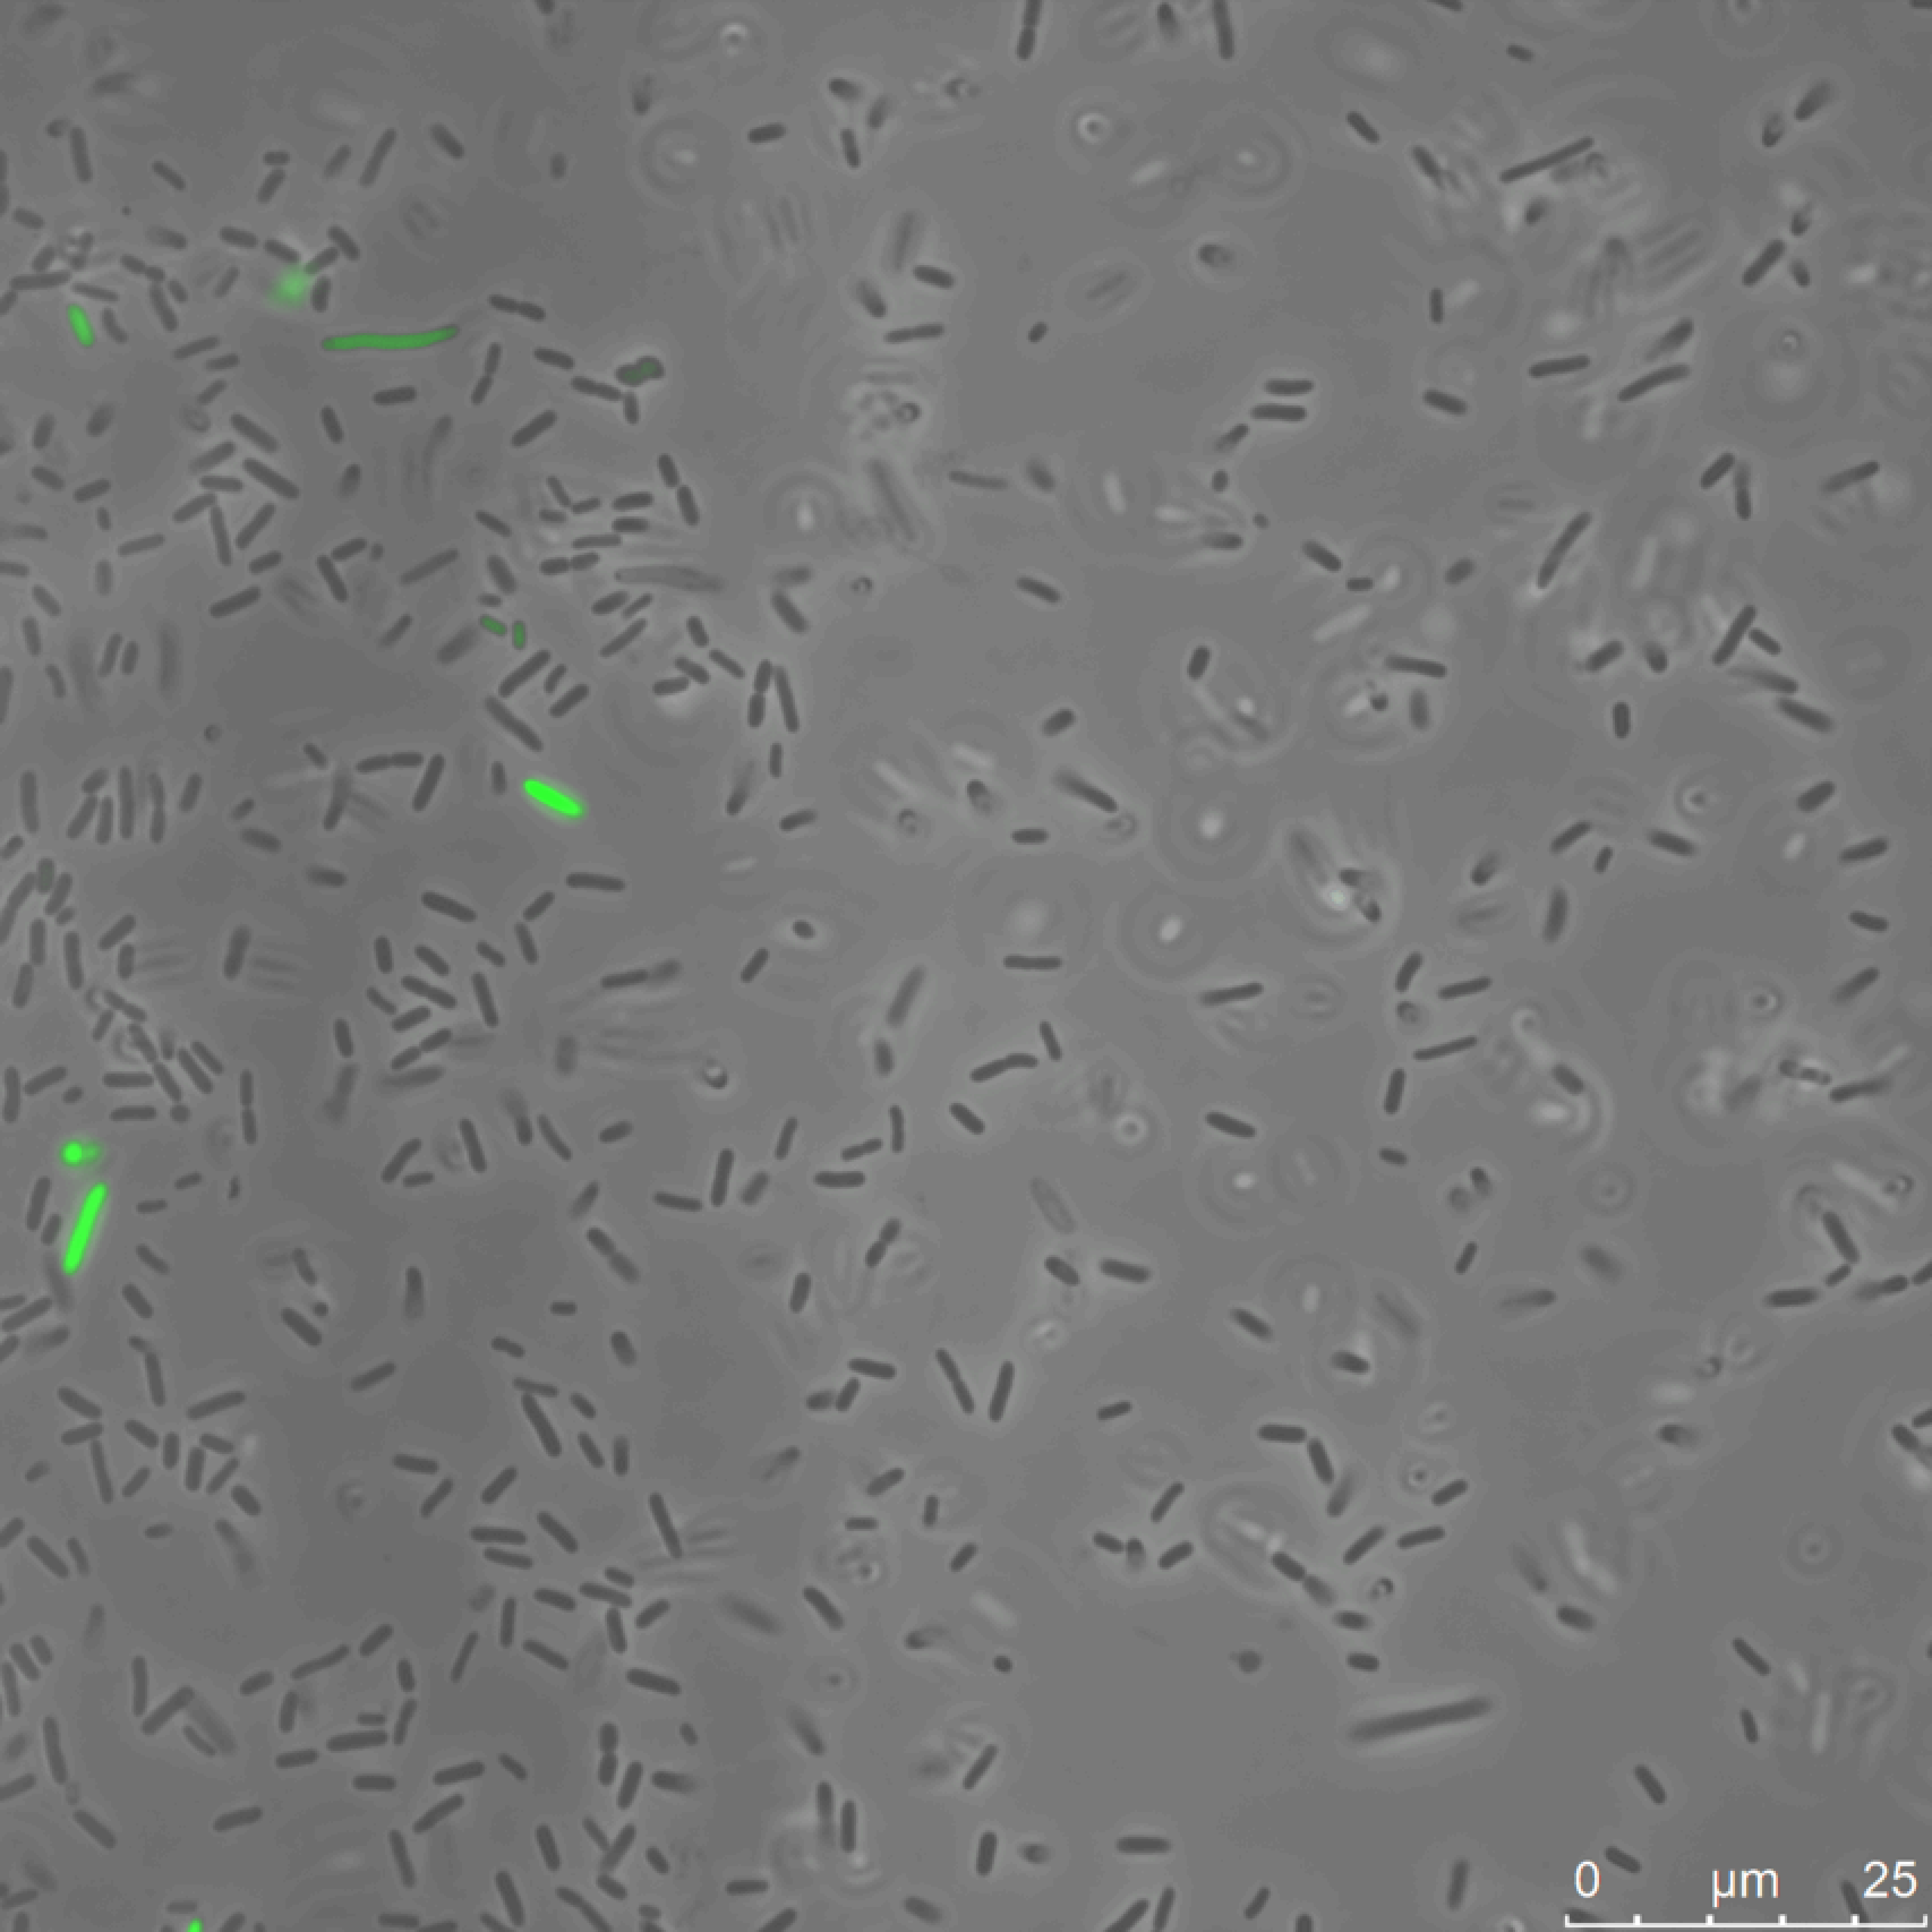
\includegraphics{THAIU1_5HR_6_GREEN-crunch-lighter-resample.pdf} &%
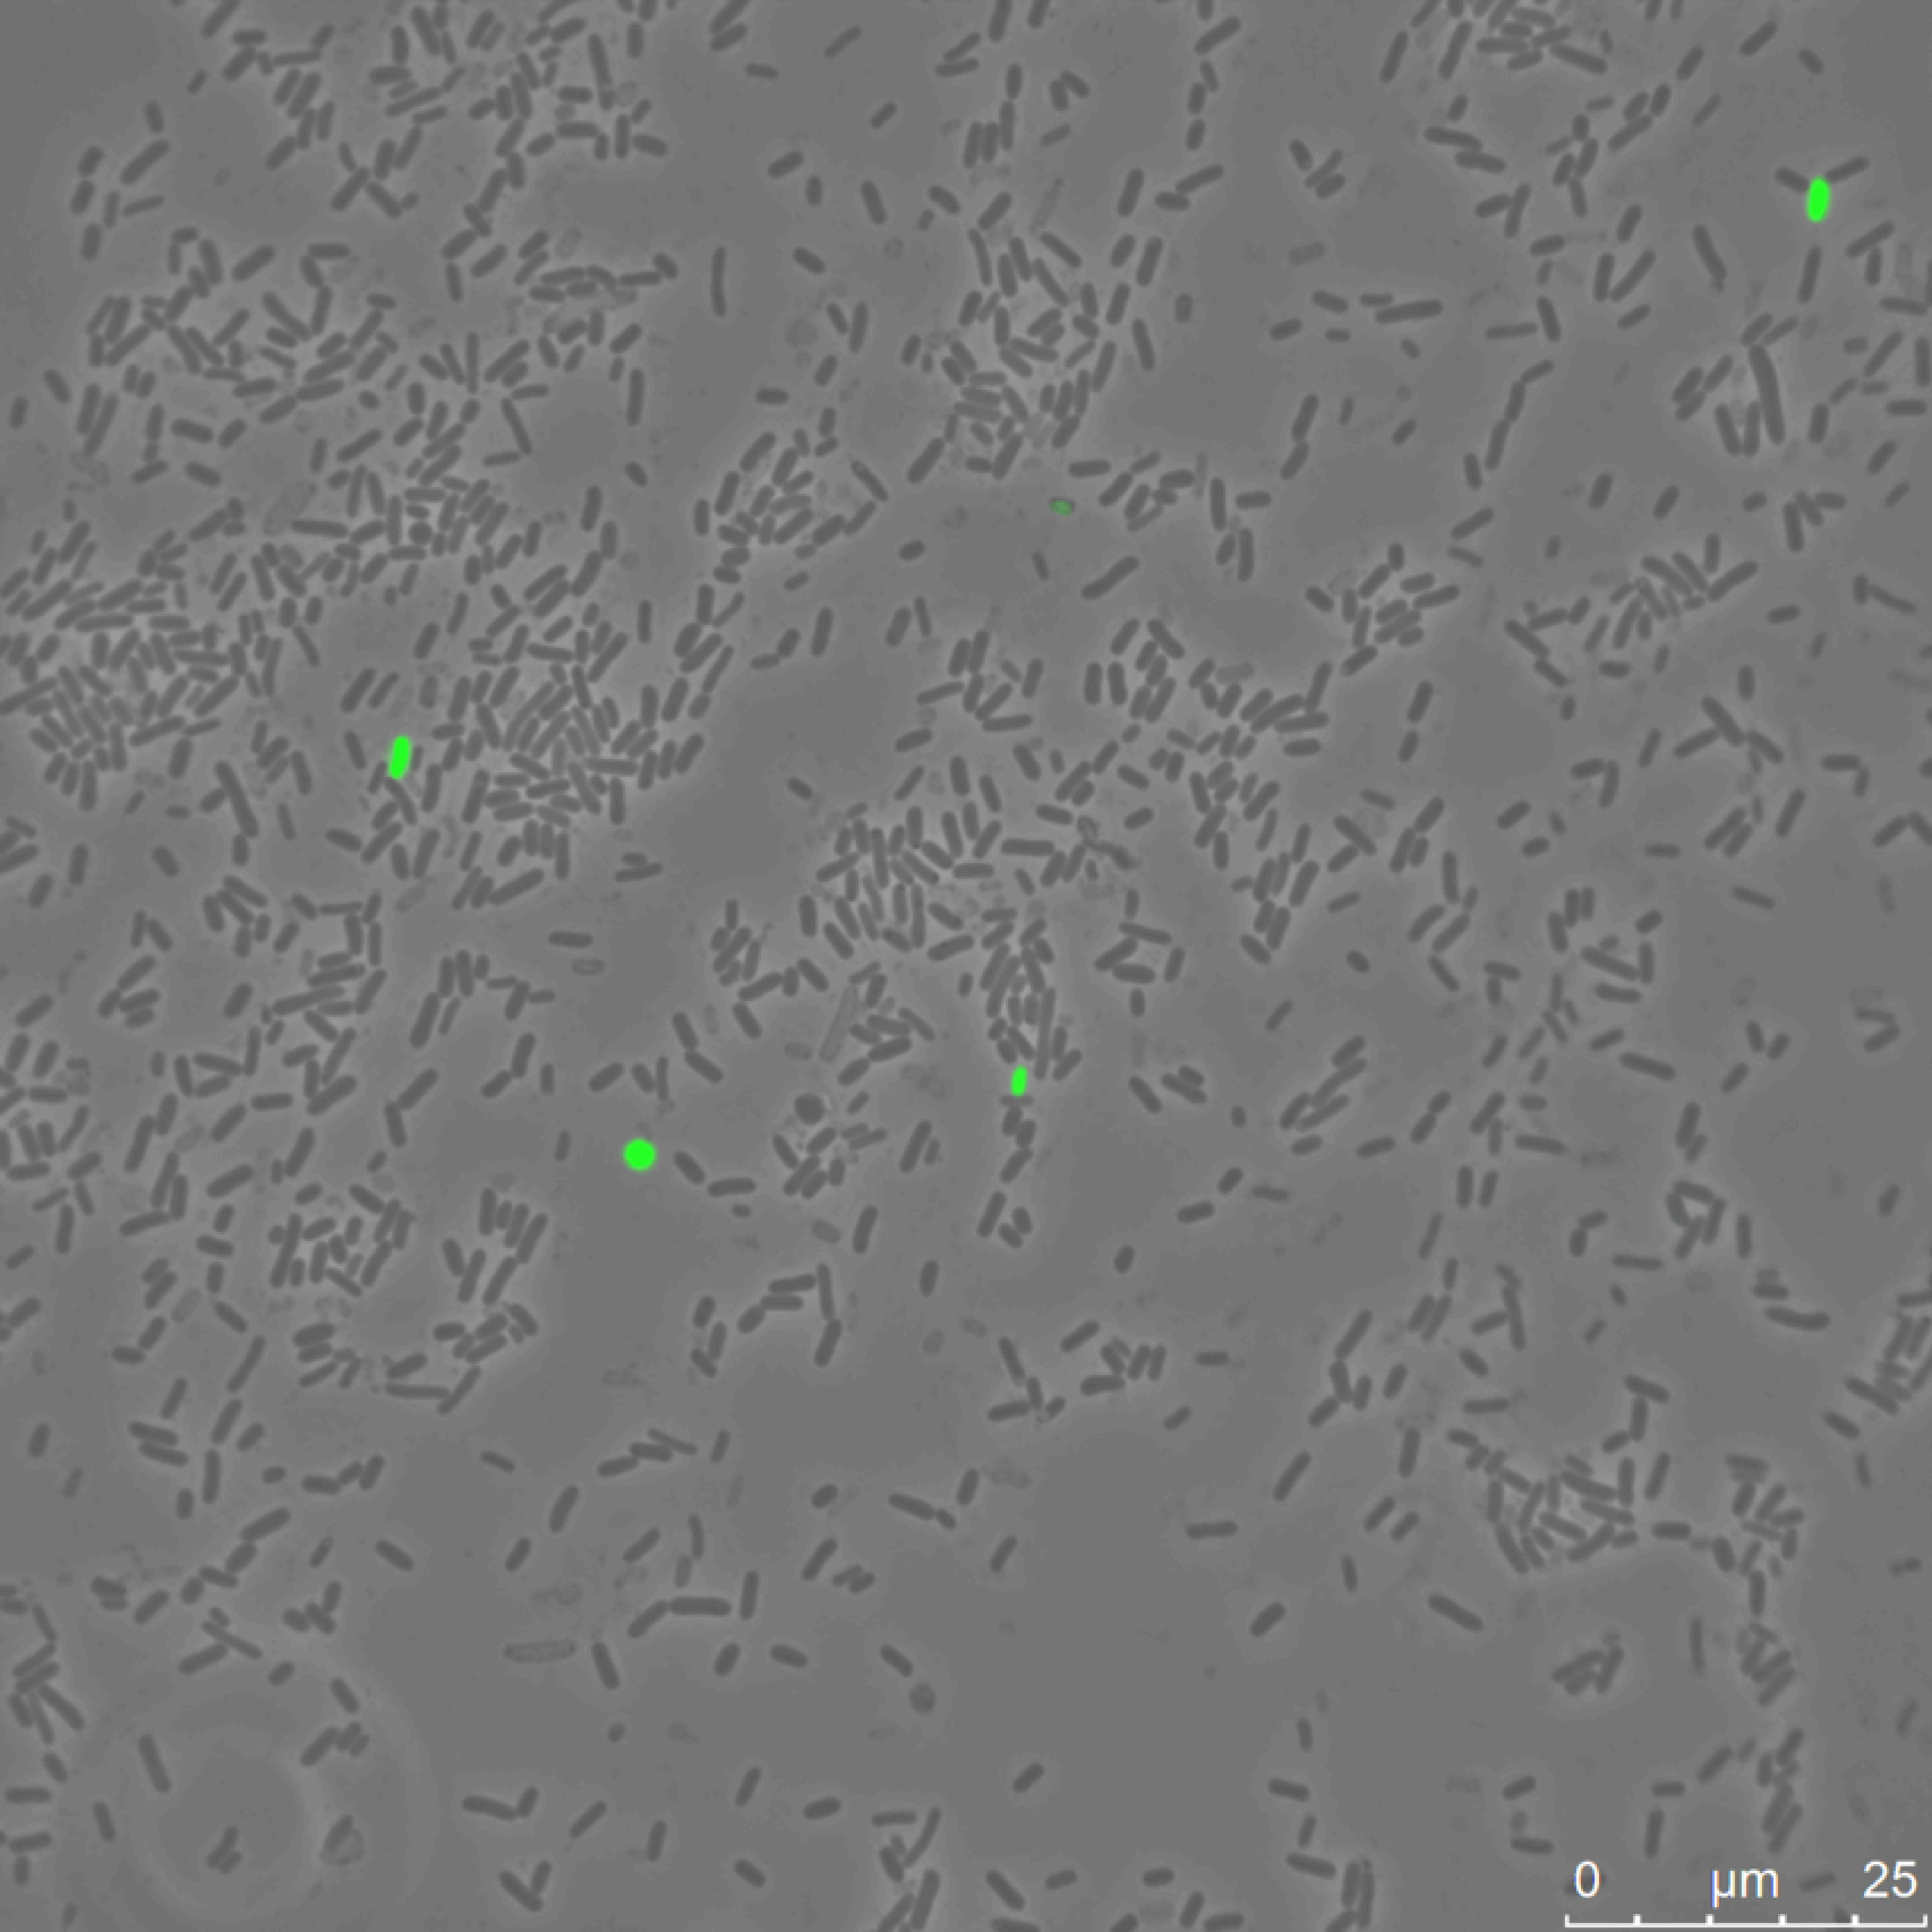
\includegraphics{THAIU1_24HR_8_GREEN-crunch-lighter-resample.pdf} &%
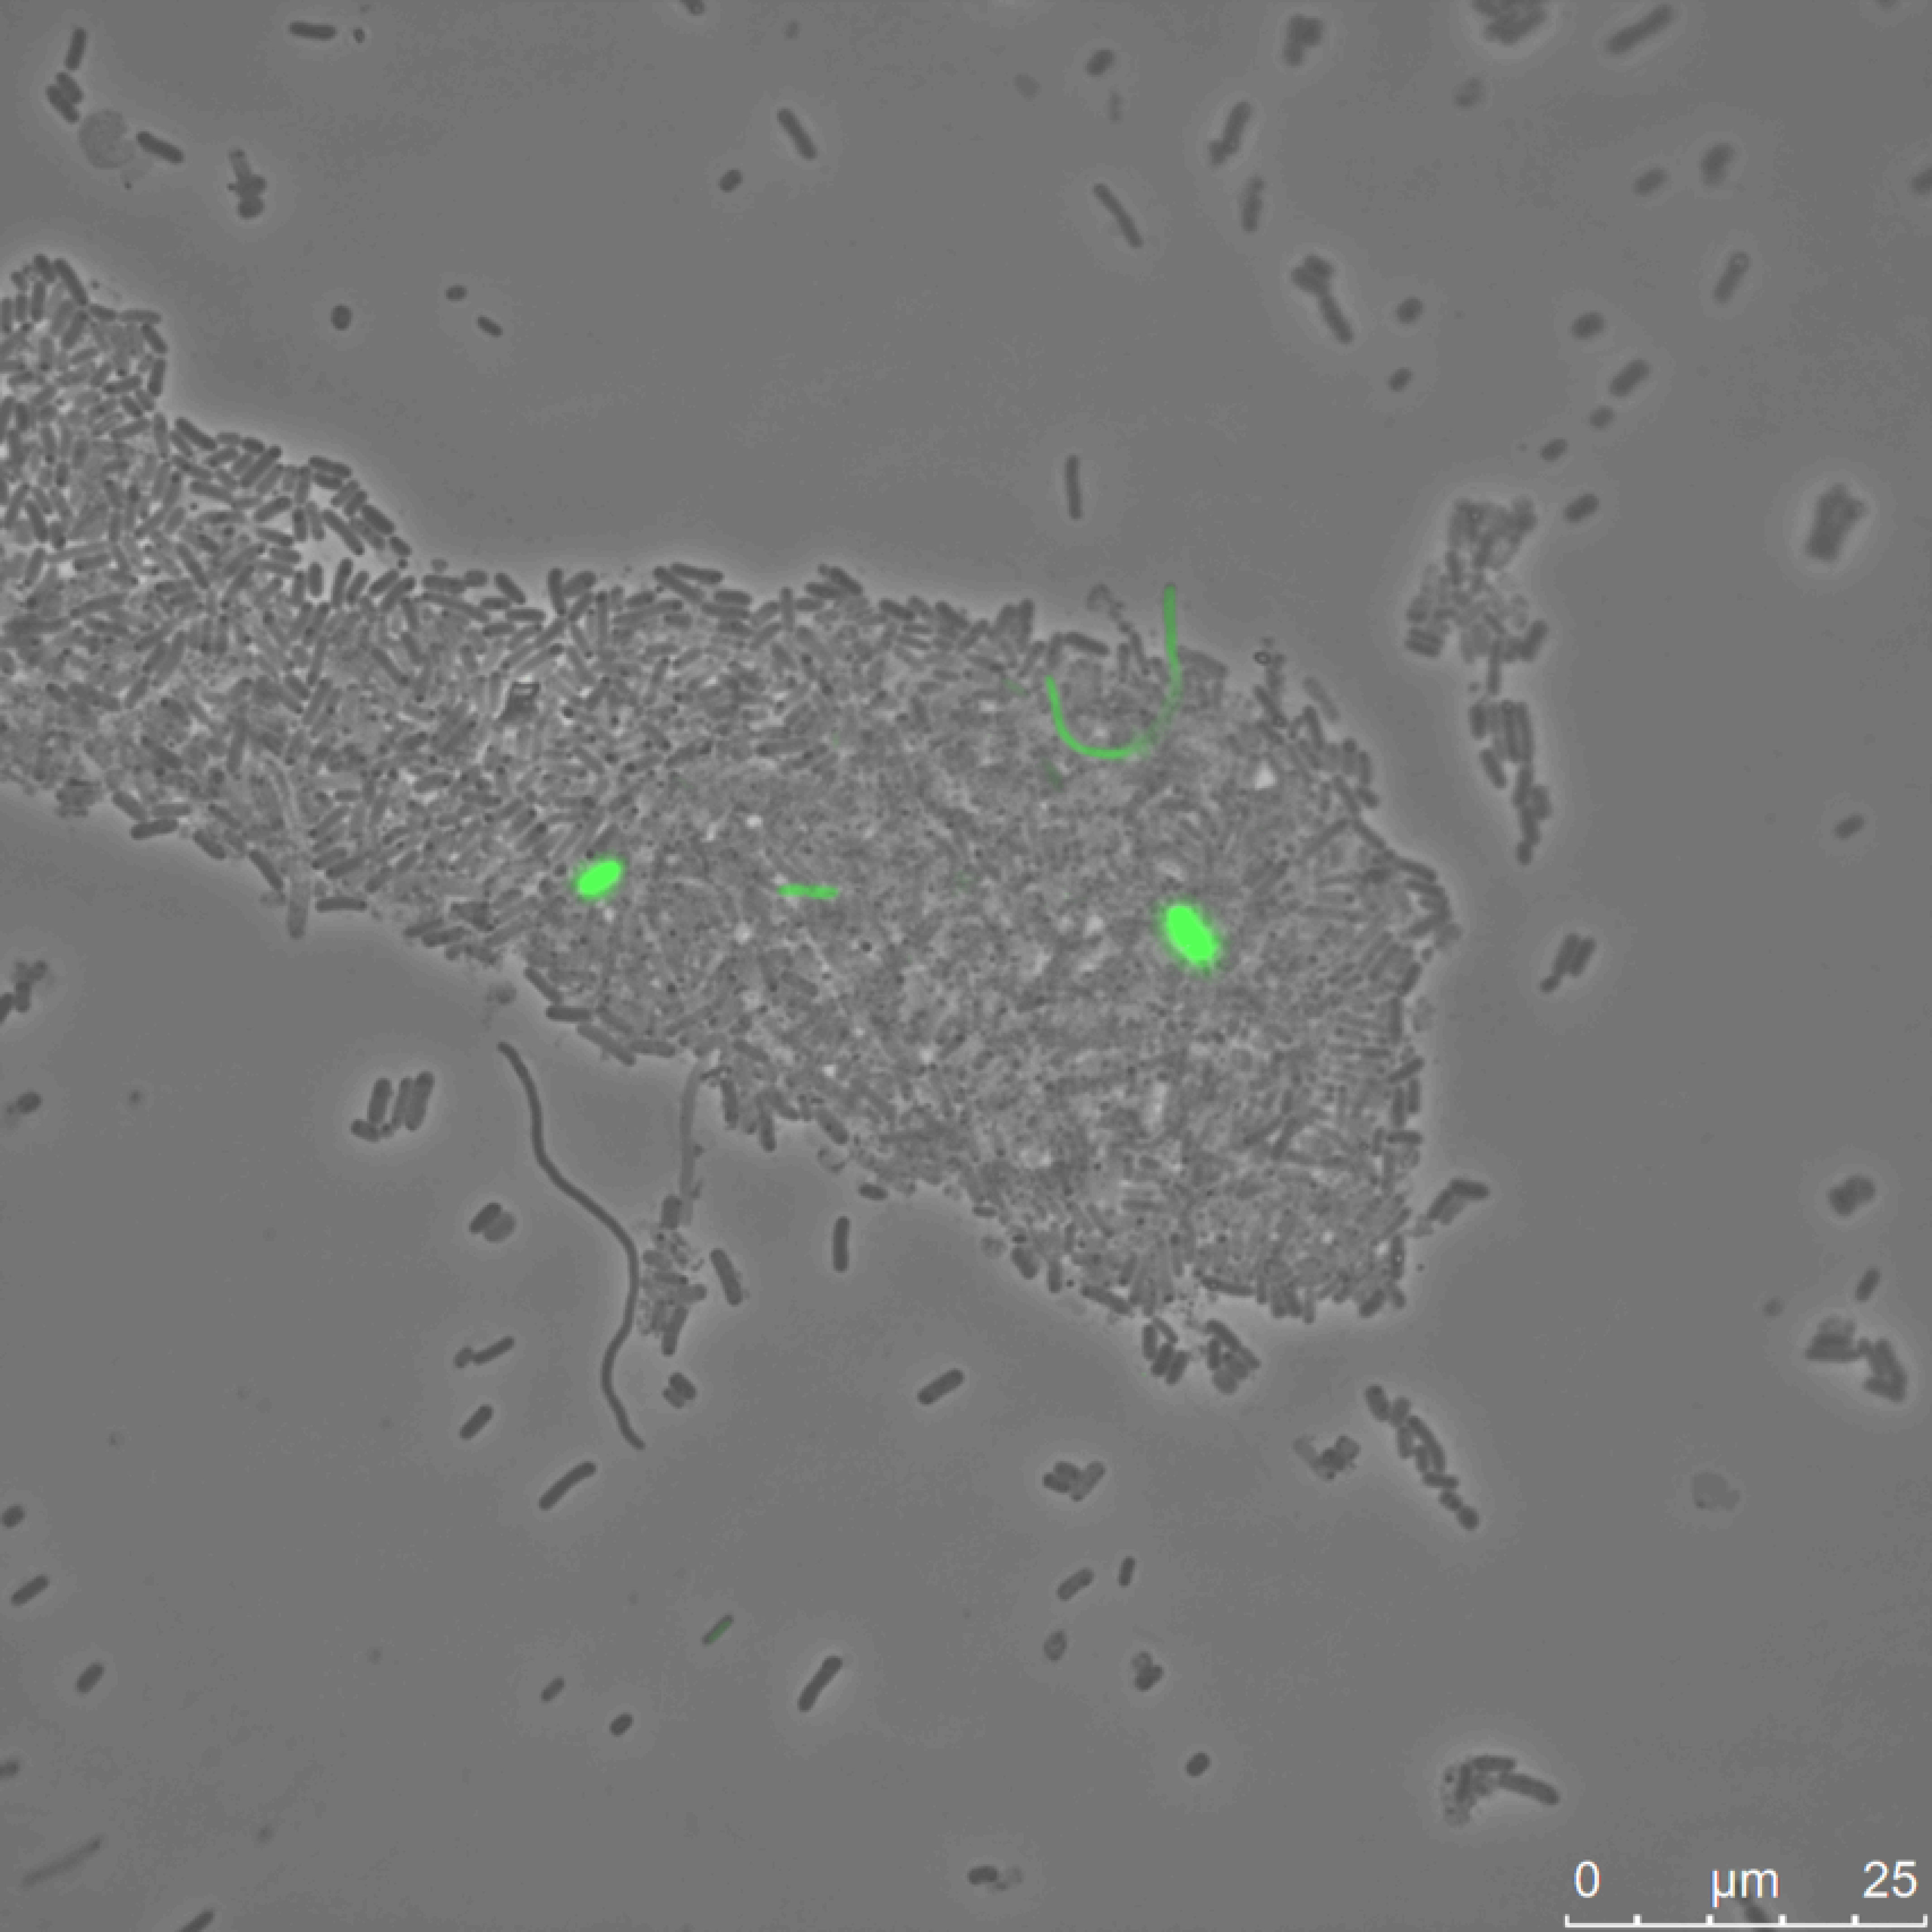
\includegraphics{THAIU1_72HR_4_GREEN-crunch-lighter-resample.pdf} \\
 ++ & ++ & ++ & ++ \\[1ex]

\end{tabularx}
\captionsetup{singlelinecheck=off, justification=justified, font=footnotesize, aboveskip=20pt}
\caption[Reporter microscopy - PB68.1 Unit 1]{\textsc{\normalsize Reporter microscopy for the \emph{P. asymbiotica} PB68.1 ``Unit 1" promoter.}\vspace{0.1cm} \newline A representative selection of images for 4 time points, for the PVC ``Unit 1" promoter fusion. Quadruplicate images are displayed vertically as representative of the whole slide sample. Key to qualitative fluorescence indication: ``-" - no fluorescence, ``+" - low level fluorescence in isolated cells. ``++" - low level fluorescence in many cells or few brighter cells, ``+++" - intermediate to high fluorescence in almost all cells, or very bright isolated cells.}
\end{figure}\label{RMTHAIU1}
\endgroup

%%%%%%%%%%%%%%%%%%%%%%%%%%%%%%%%%%%%%%%%%%%%%%%%%%%%%%%%%%%%%%%%%%%%

\begingroup
\renewcommand{\arraystretch}{0.8}%
\setlength{\tabcolsep}{0.3pt}
\begin{figure}[p]
\setkeys{Gin}{width=\linewidth}
\Huge
\begin{tabularx}{\textwidth}{CCCC}
\multicolumn{4}{p{\linewidth}}{\large \centering \textbf{\emph{P. luminescens} TT01 PVC ``Unit 4"}} \\
\hiderowcolors
& & & \\[-1.5ex]
\Large 2 Hours &\Large 5 Hours &\Large 24 Hours &\Large 72 Hours \\[1ex]

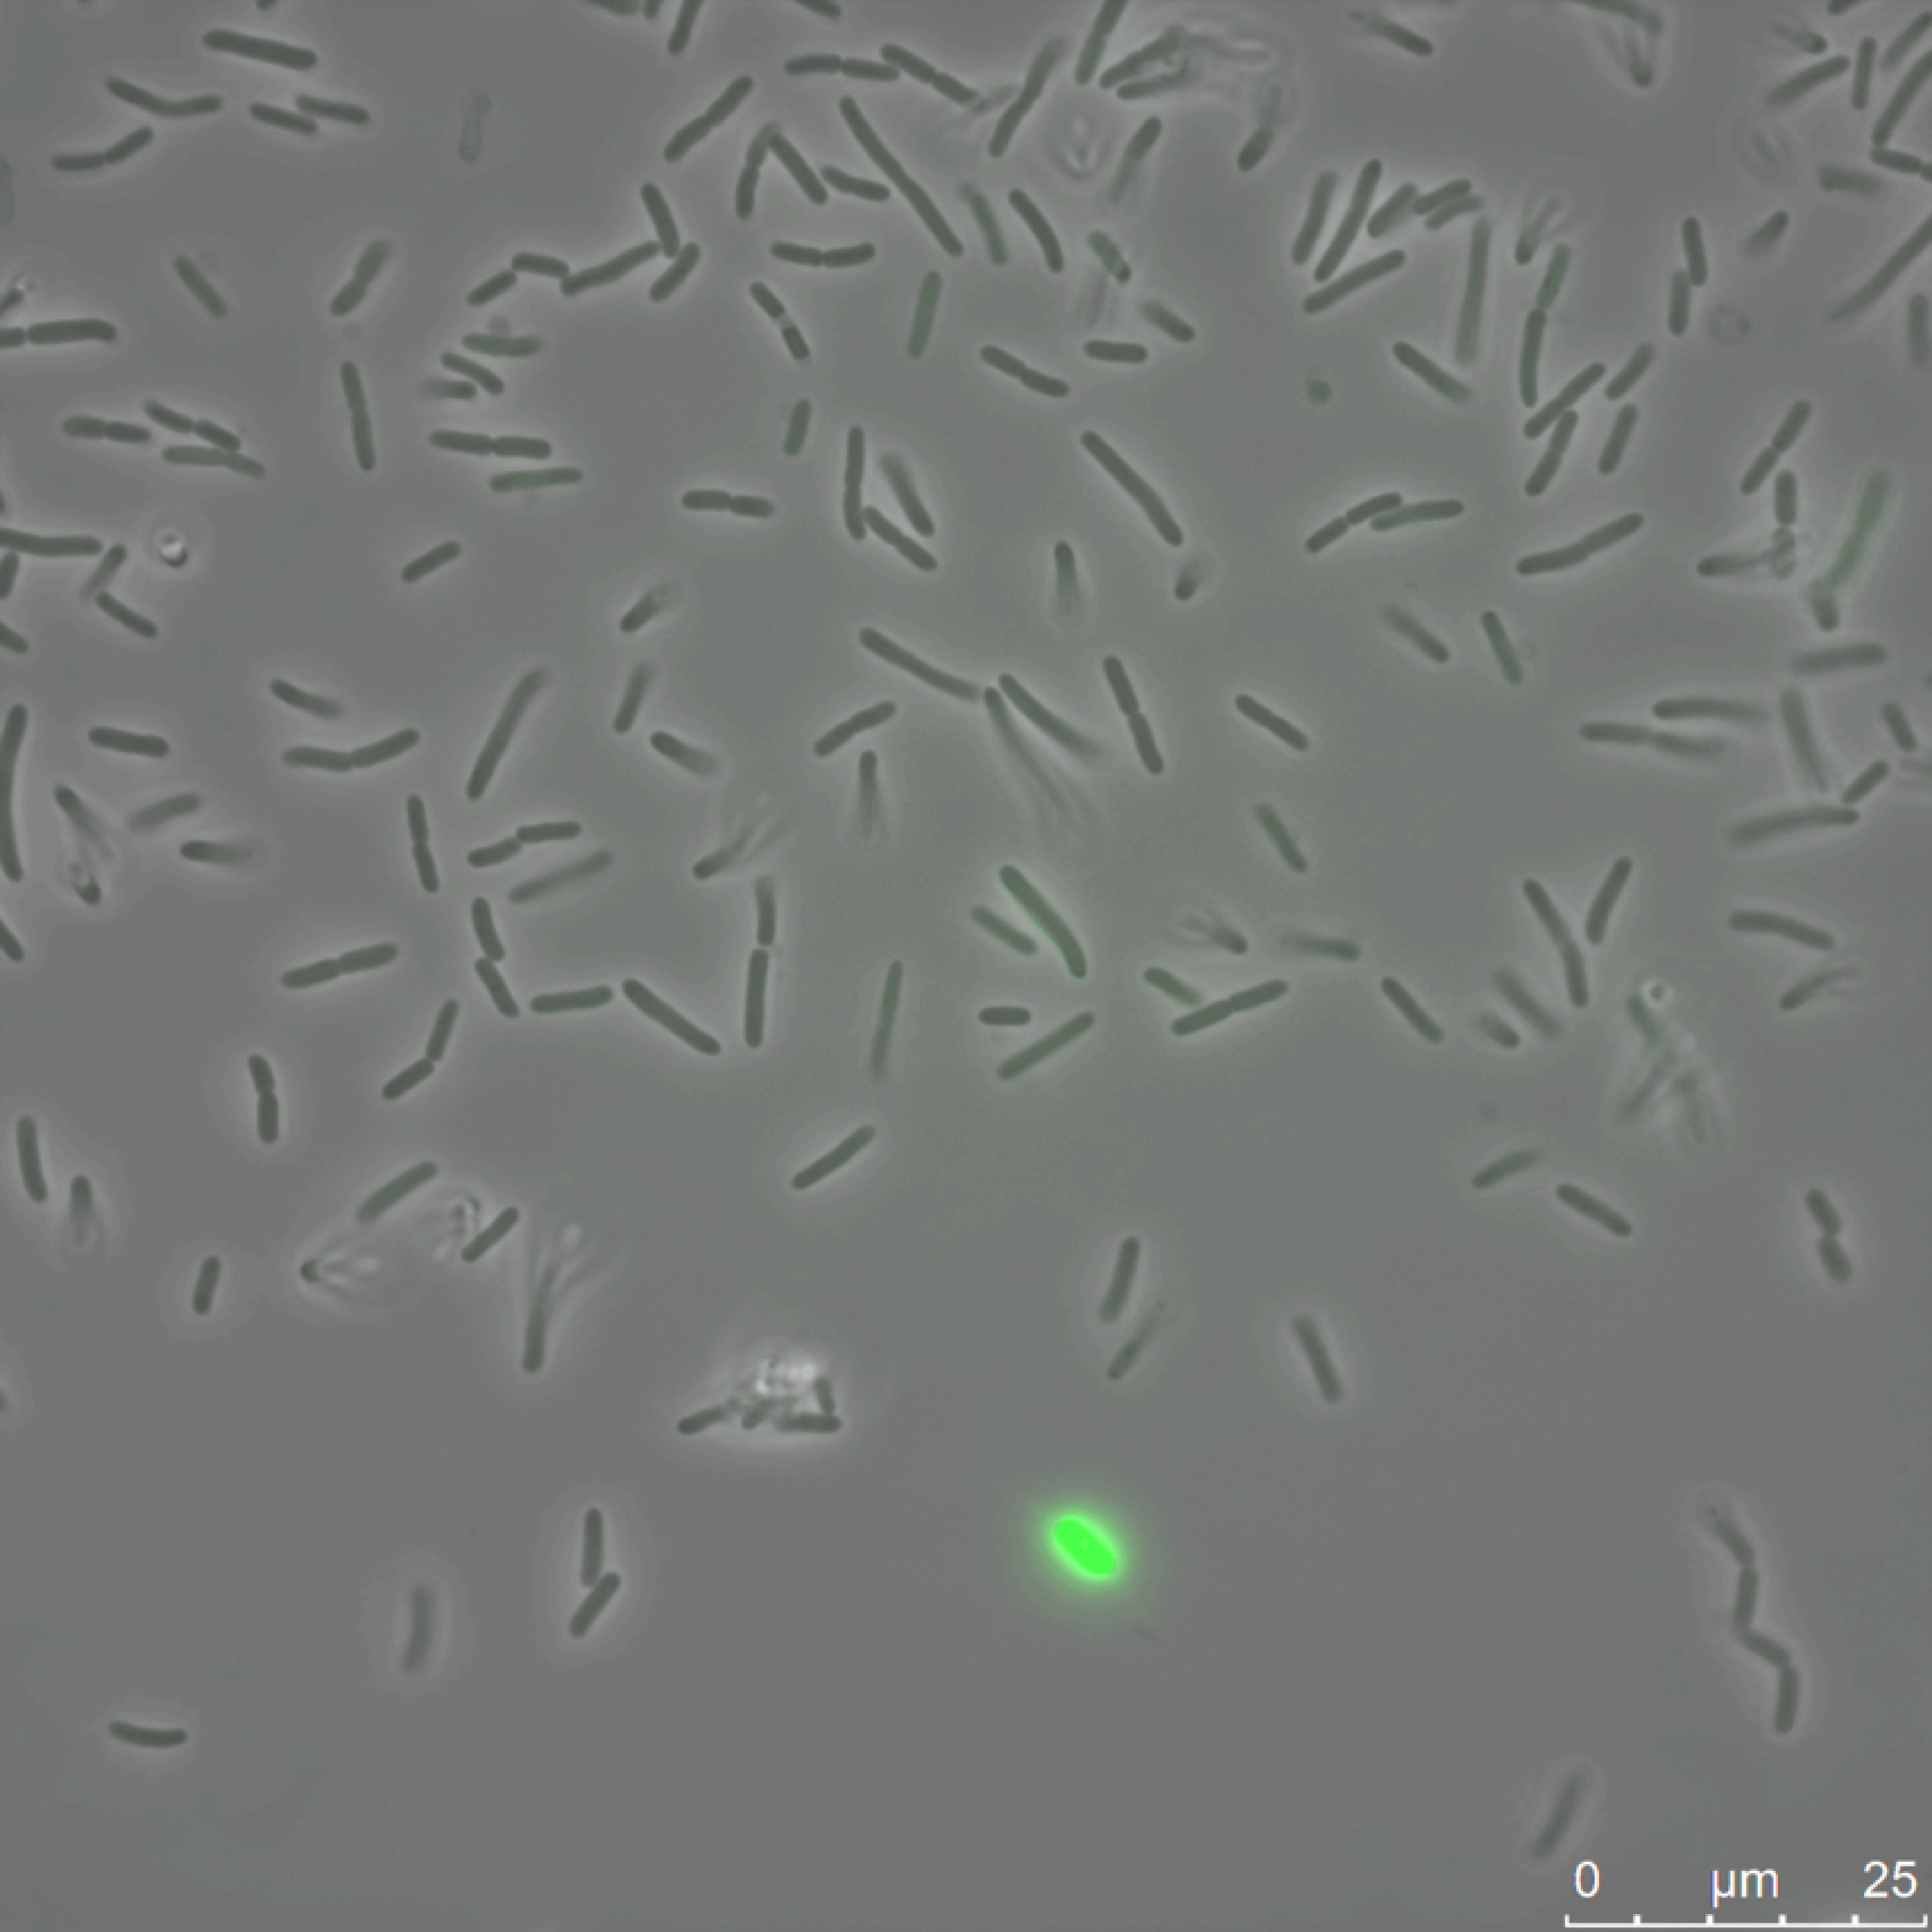
\includegraphics{TT01U4_1_GREEN-crunch-lighter-resample.pdf} &%
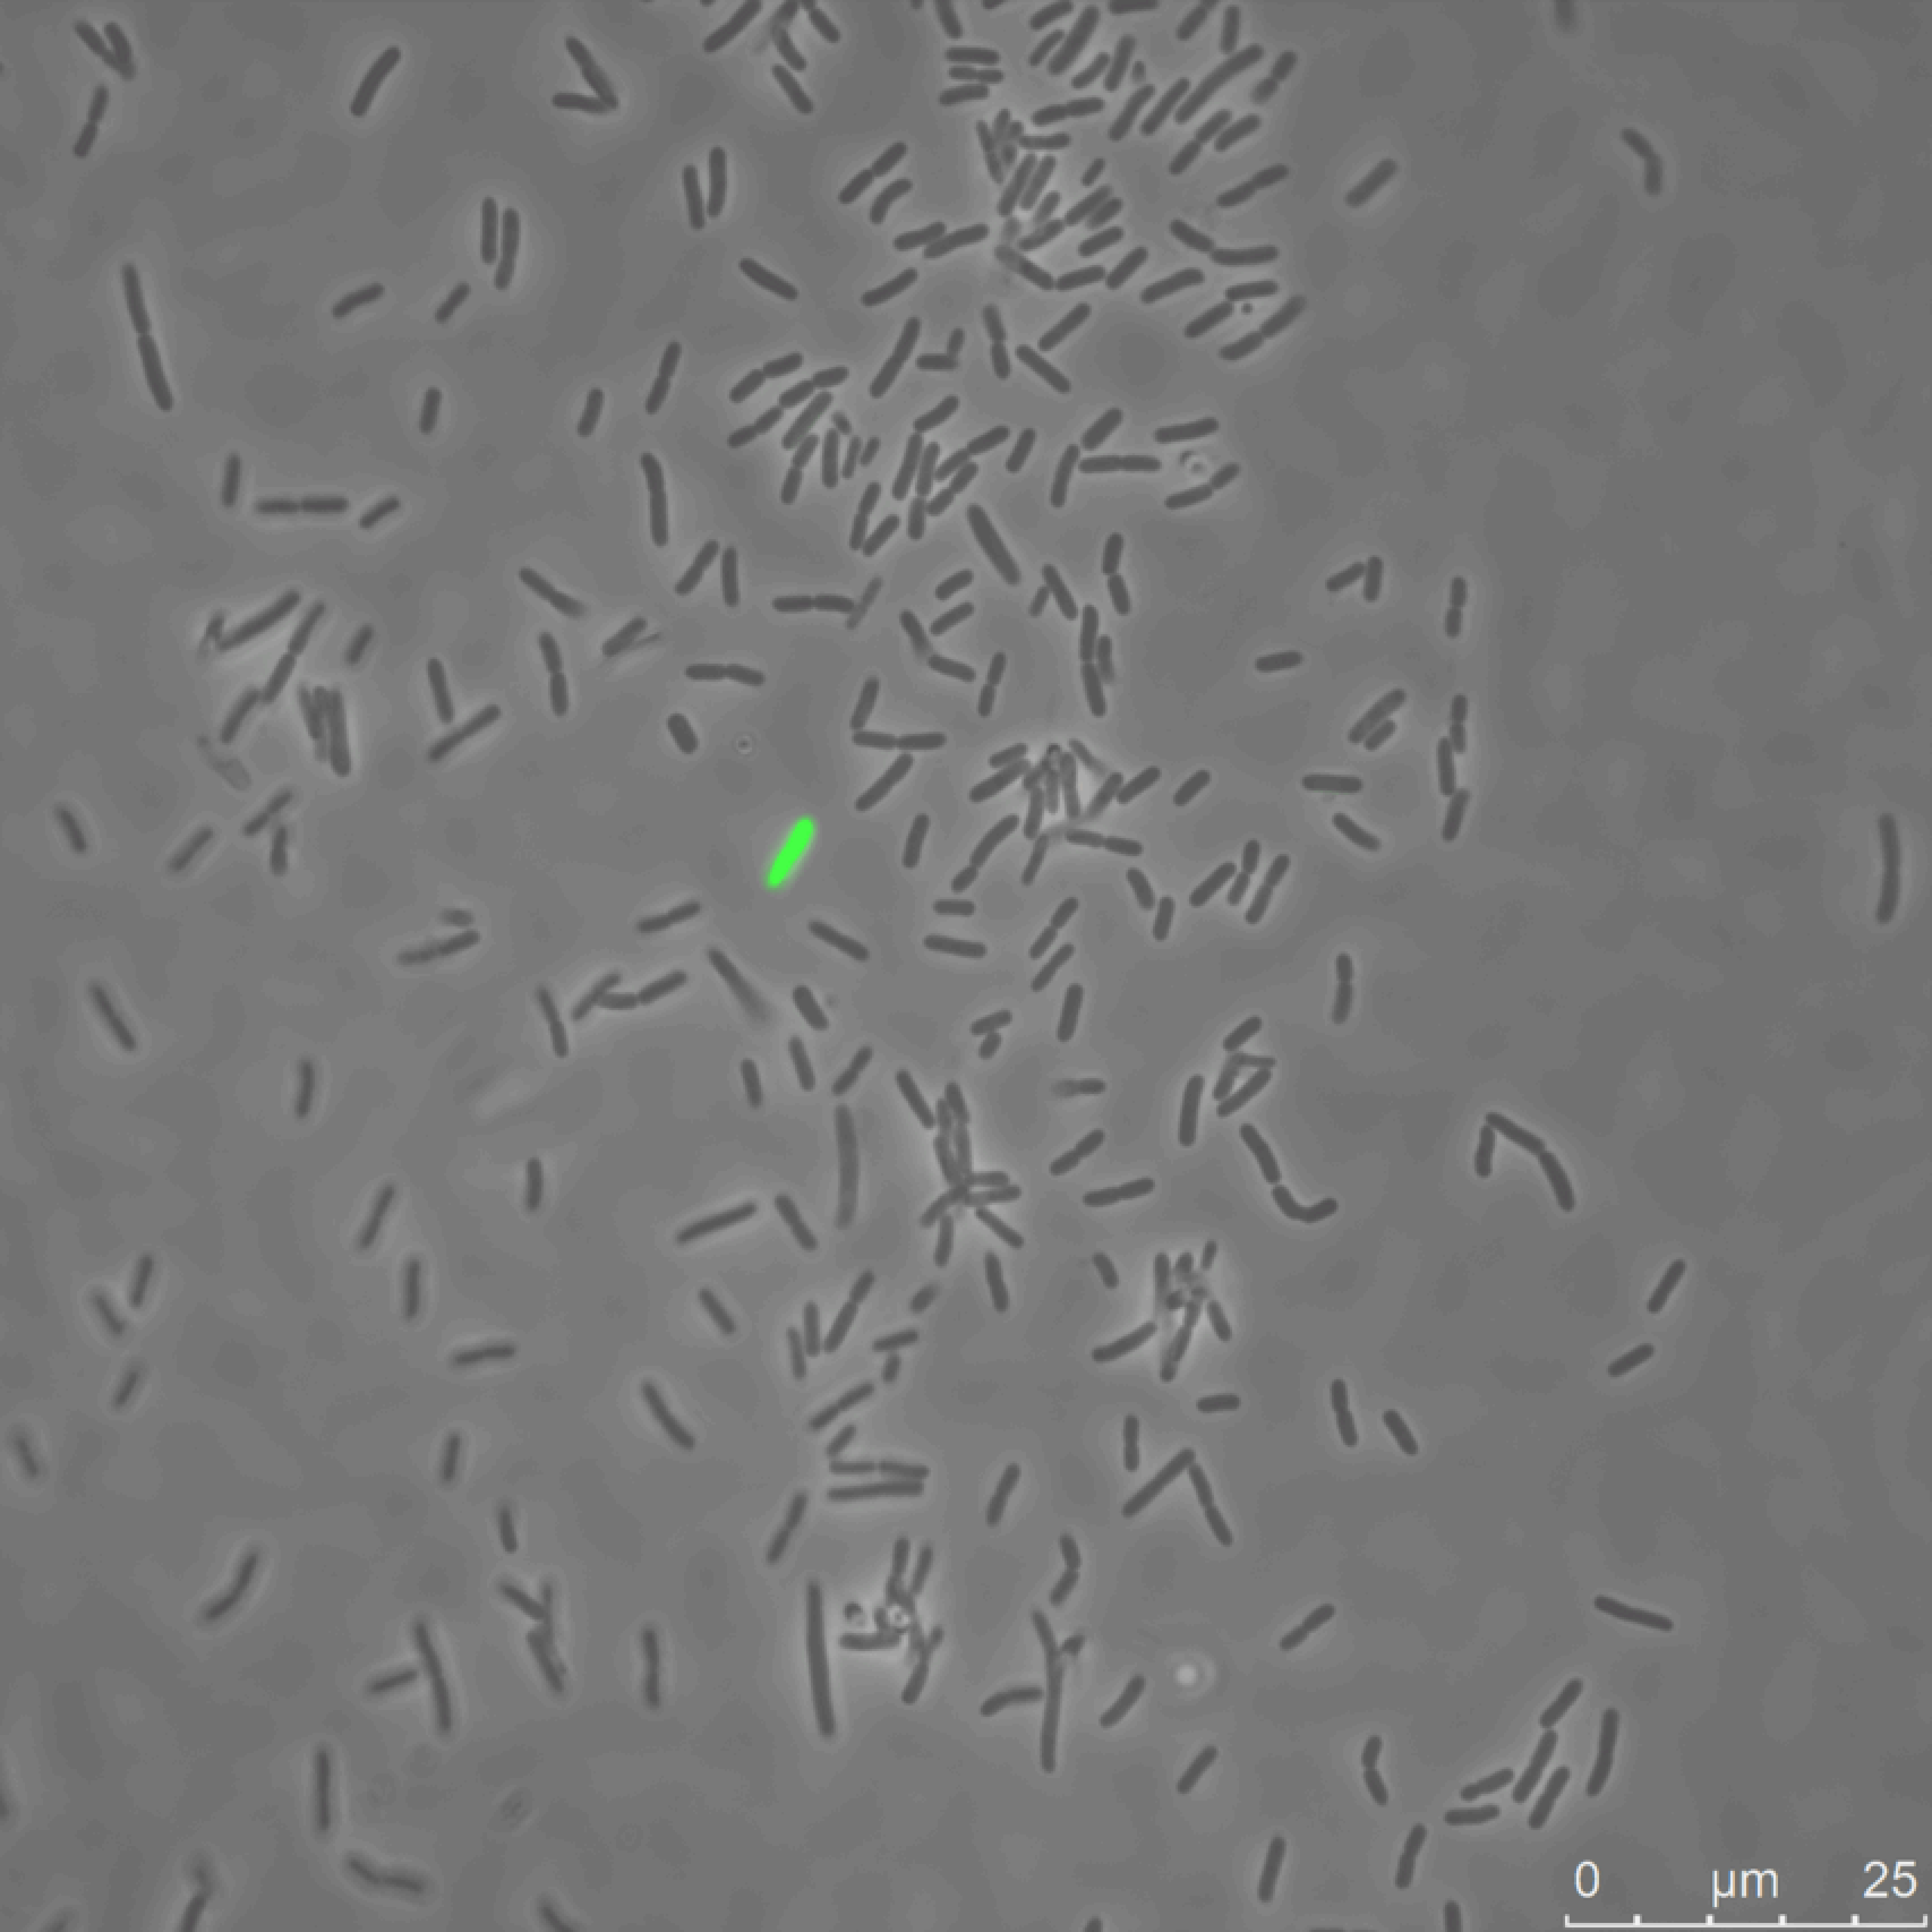
\includegraphics{TT01U4_5HR_1_GREEN-crunch-lighter-resample.pdf} &%
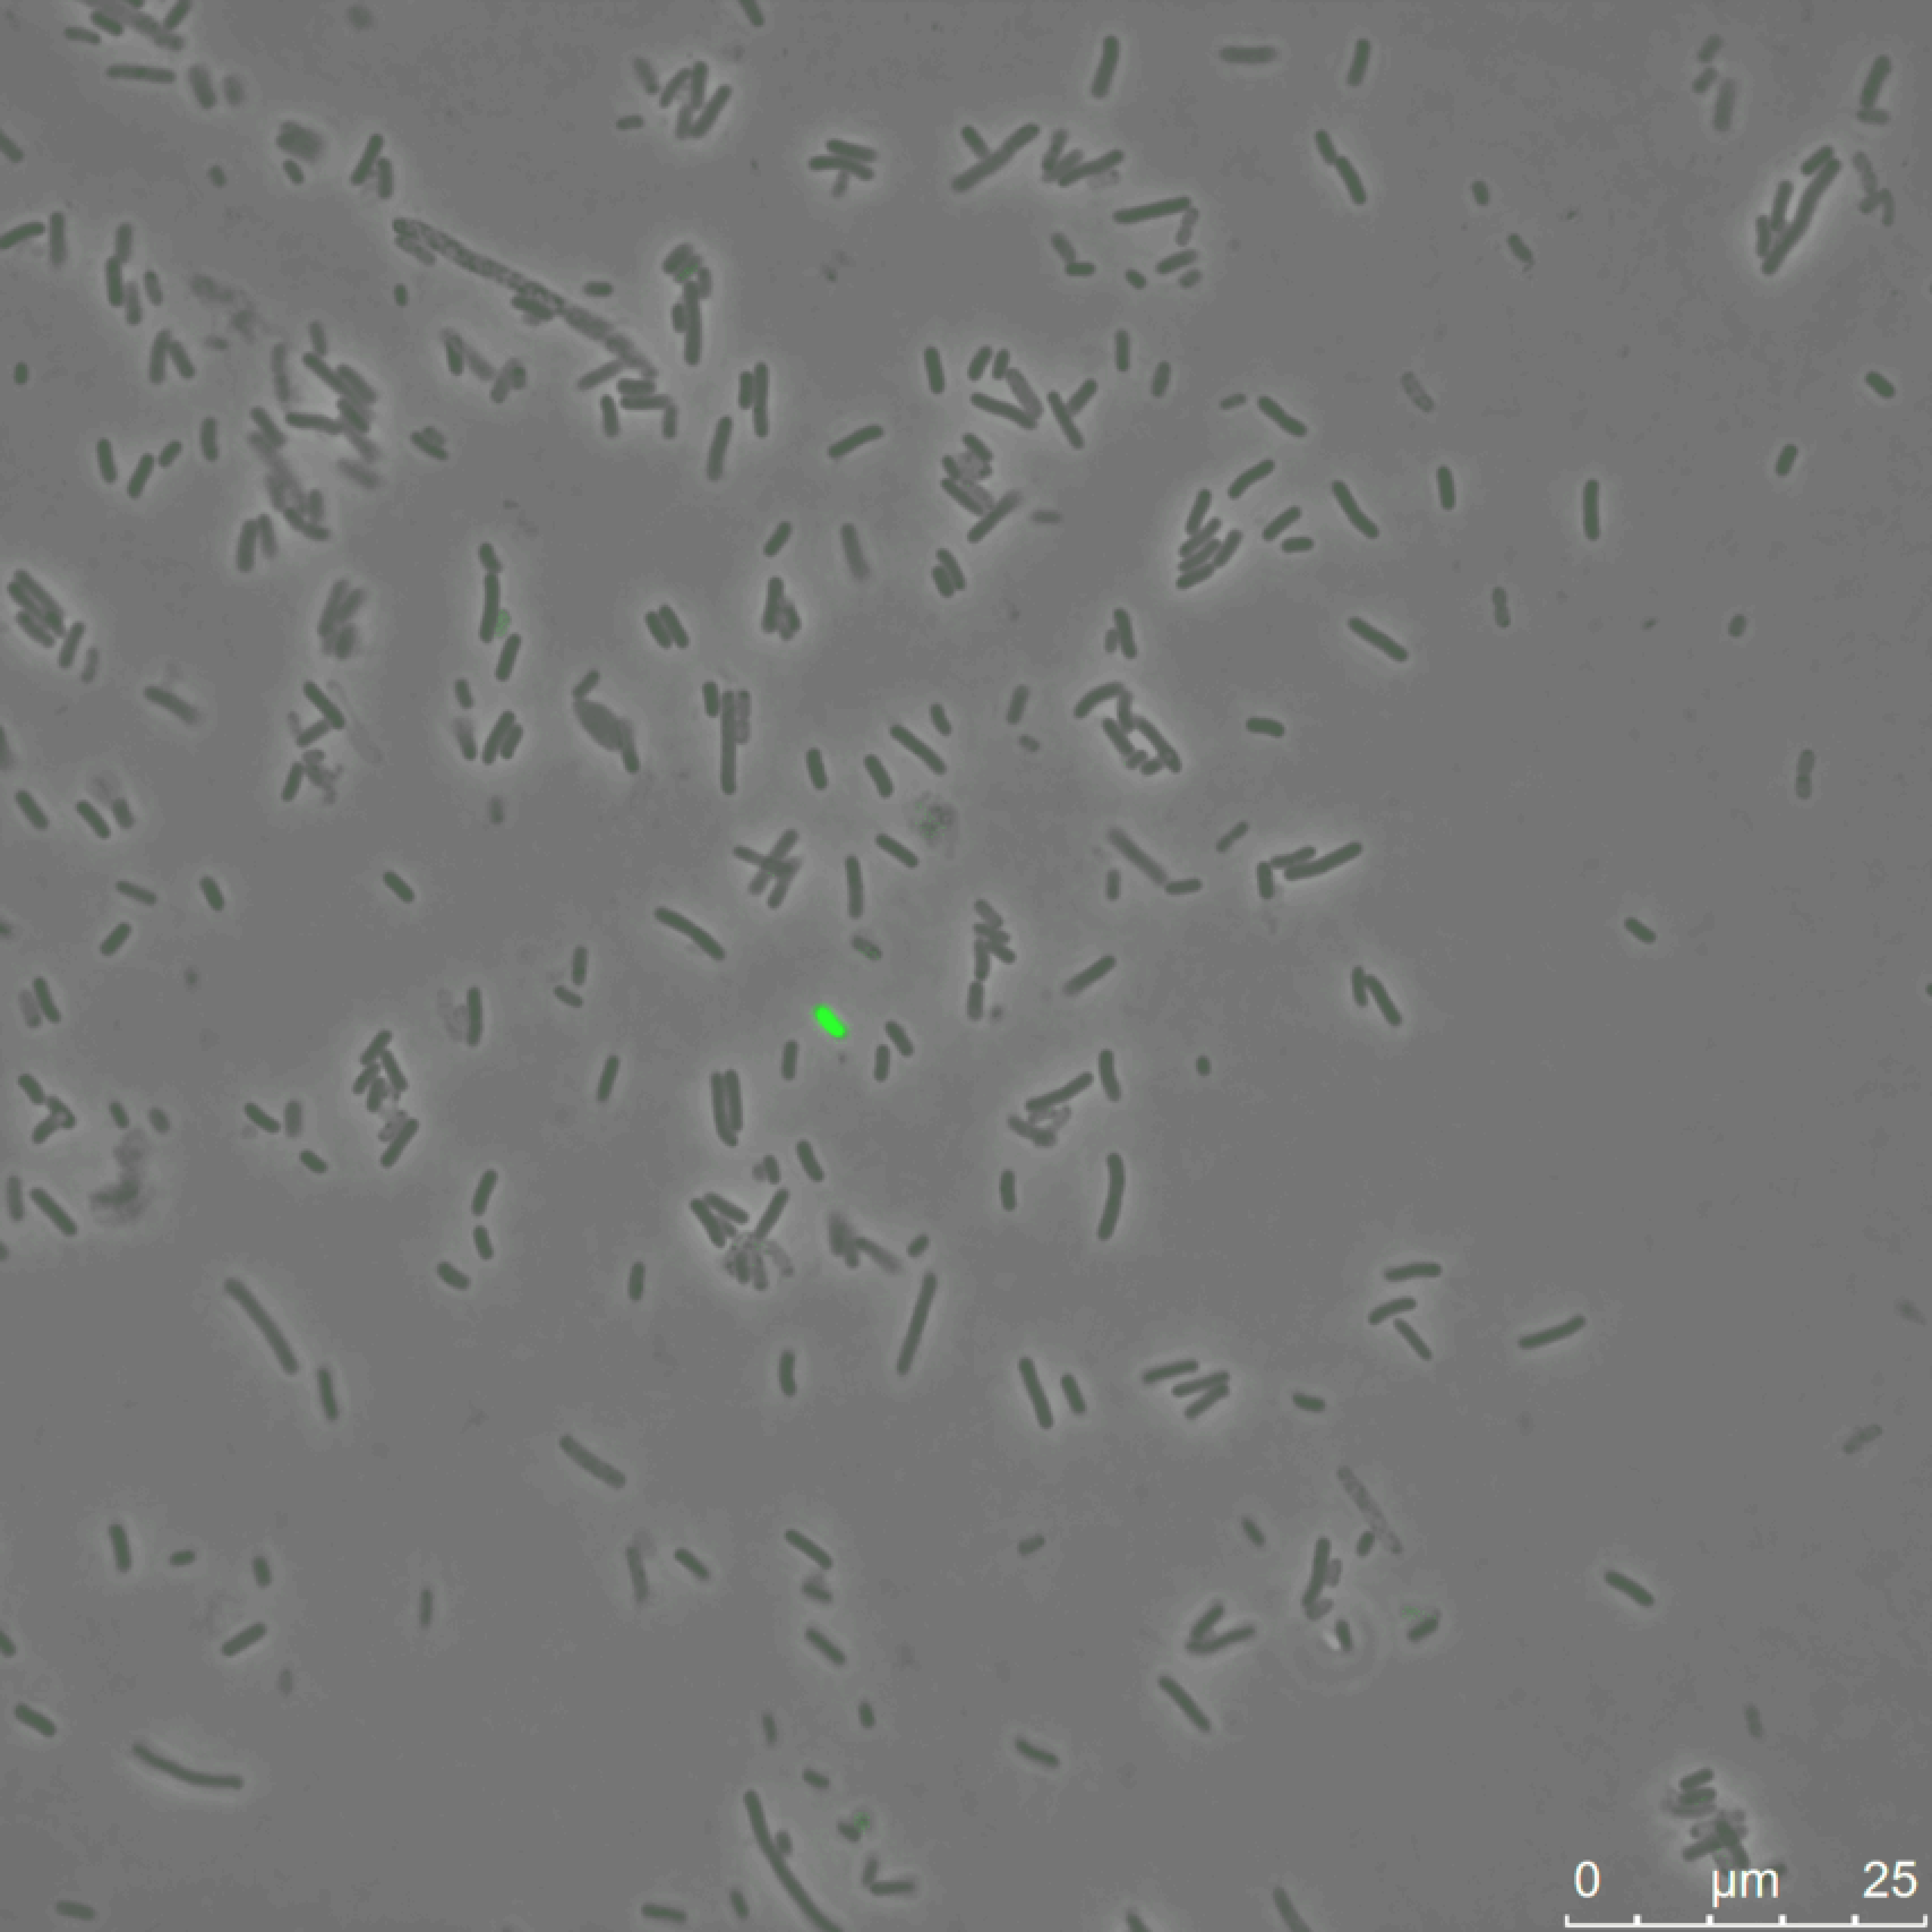
\includegraphics{TT01U4_24HR_1_GREEN-crunch-lighter-resample.pdf} &%
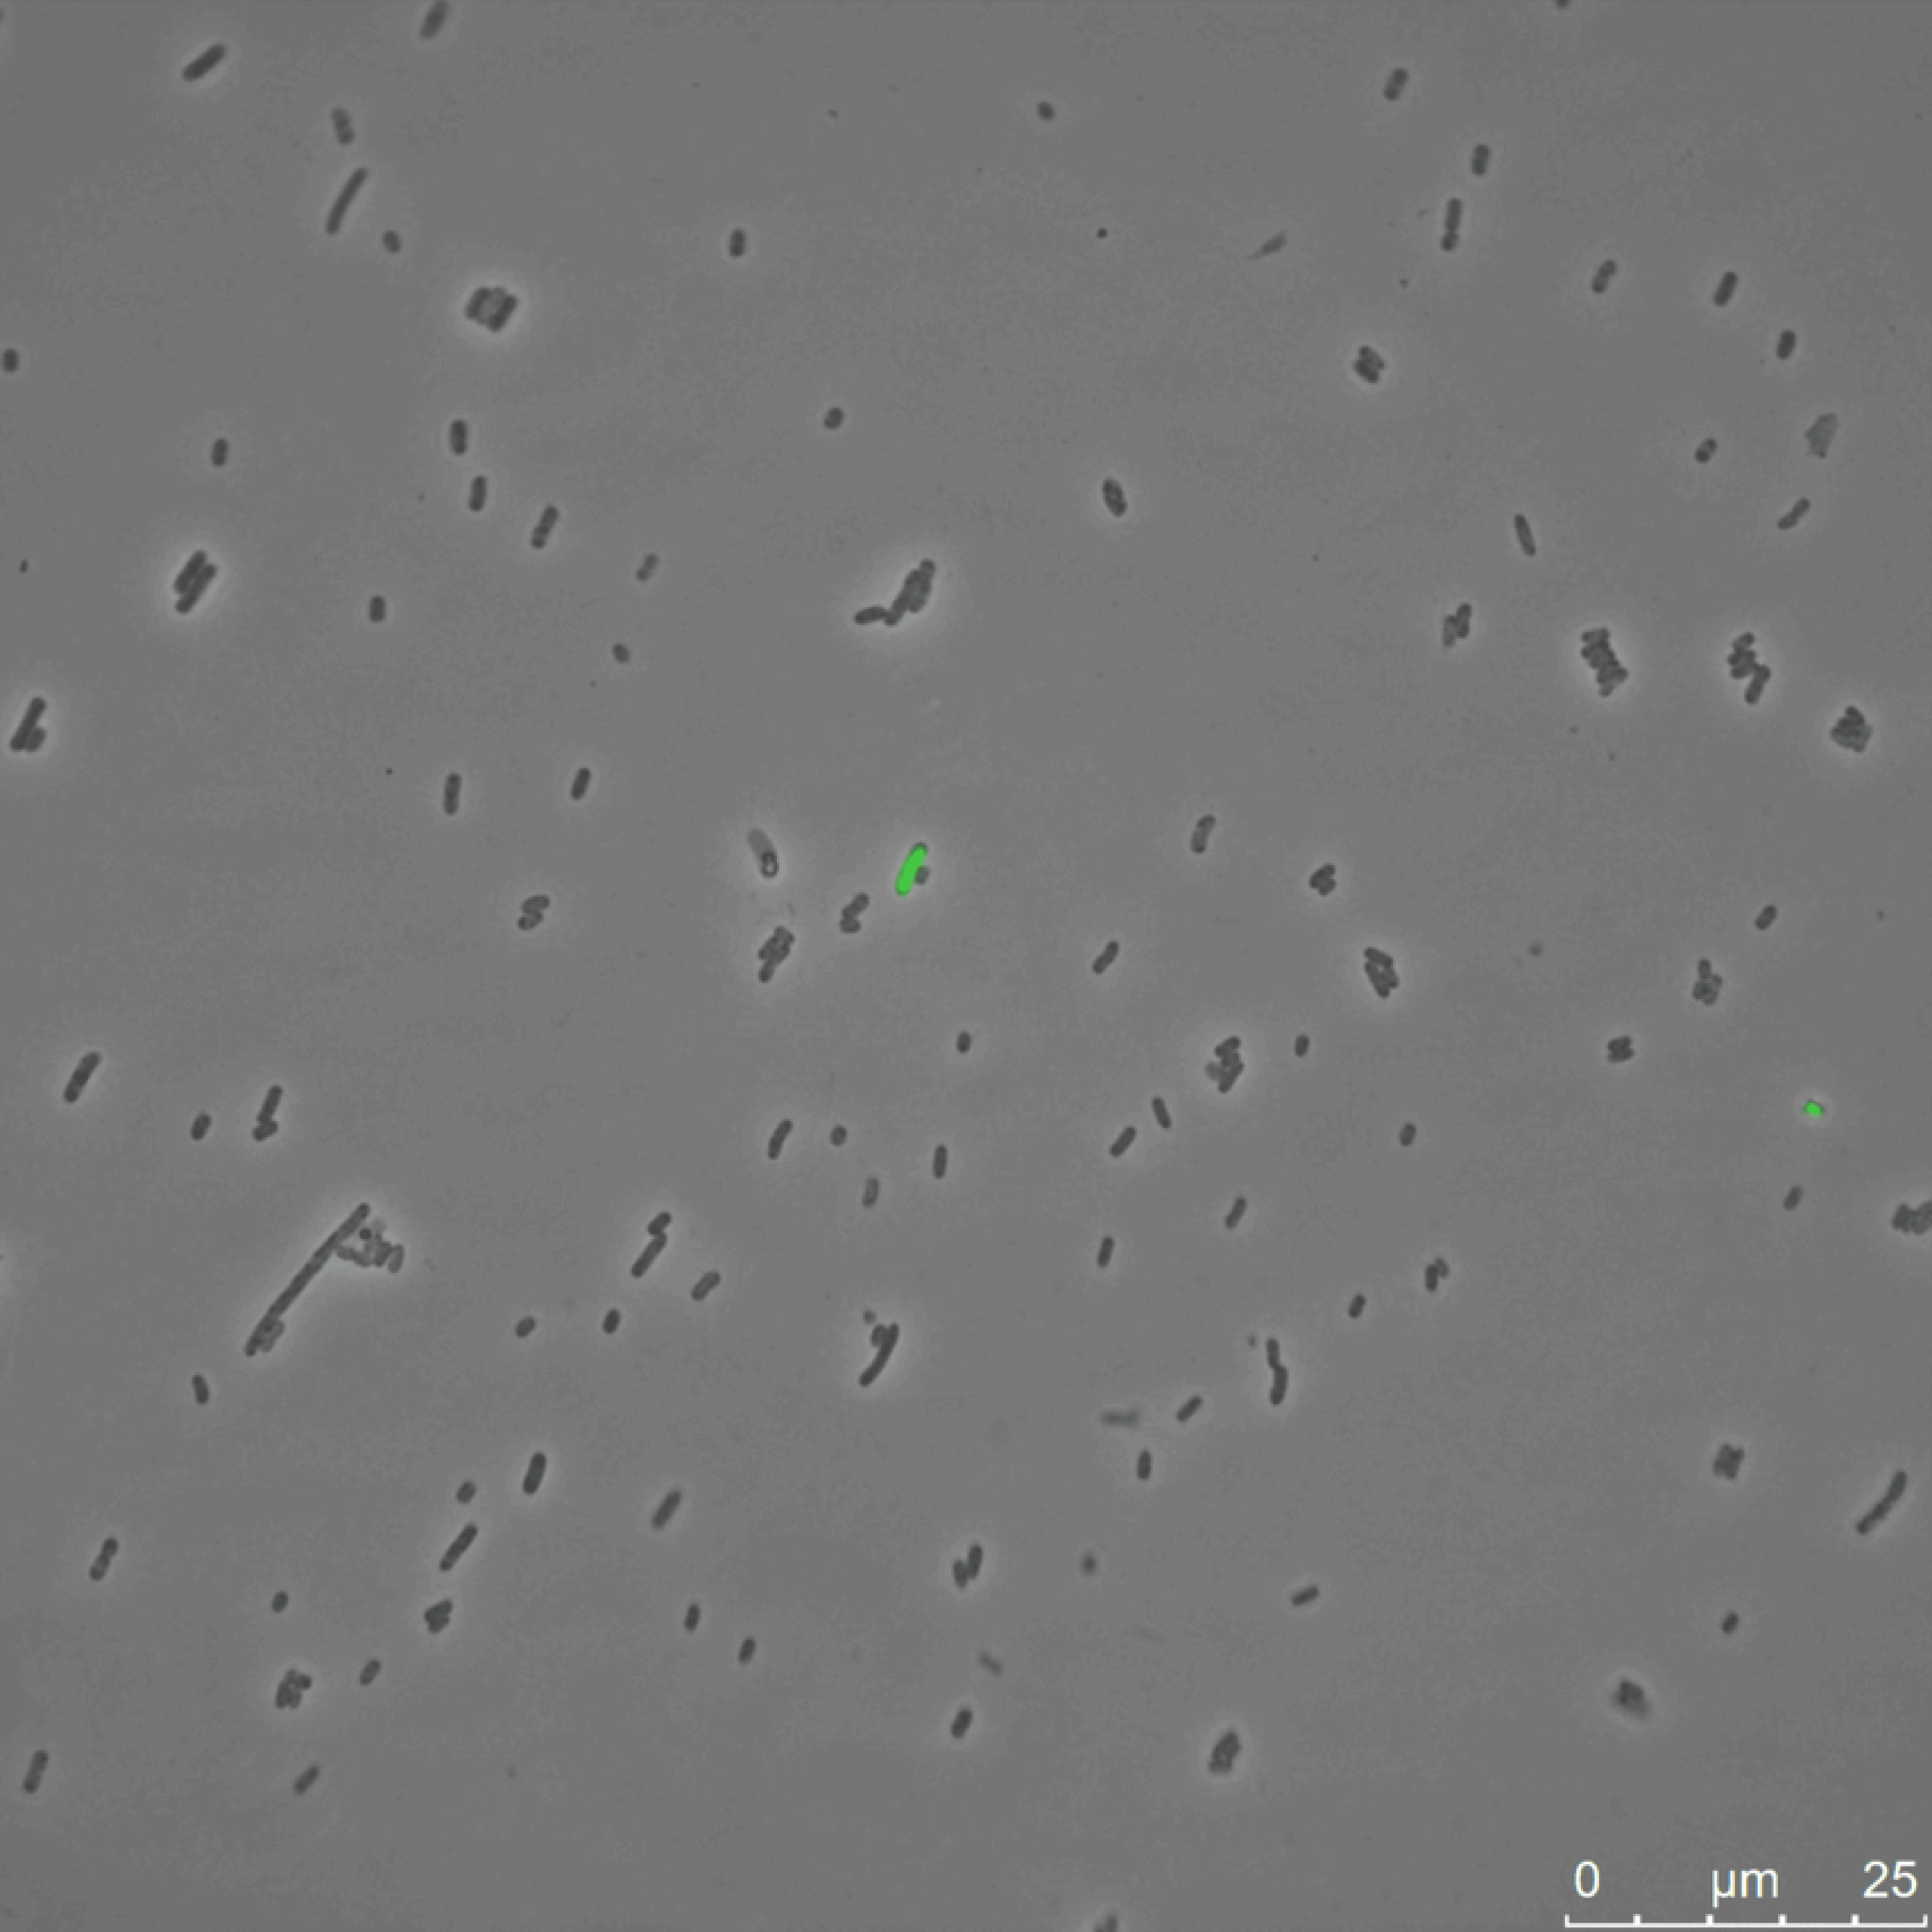
\includegraphics{TT01U4_72HR_1_GREEN-crunch-lighter-resample.pdf} \\[-0.5ex]

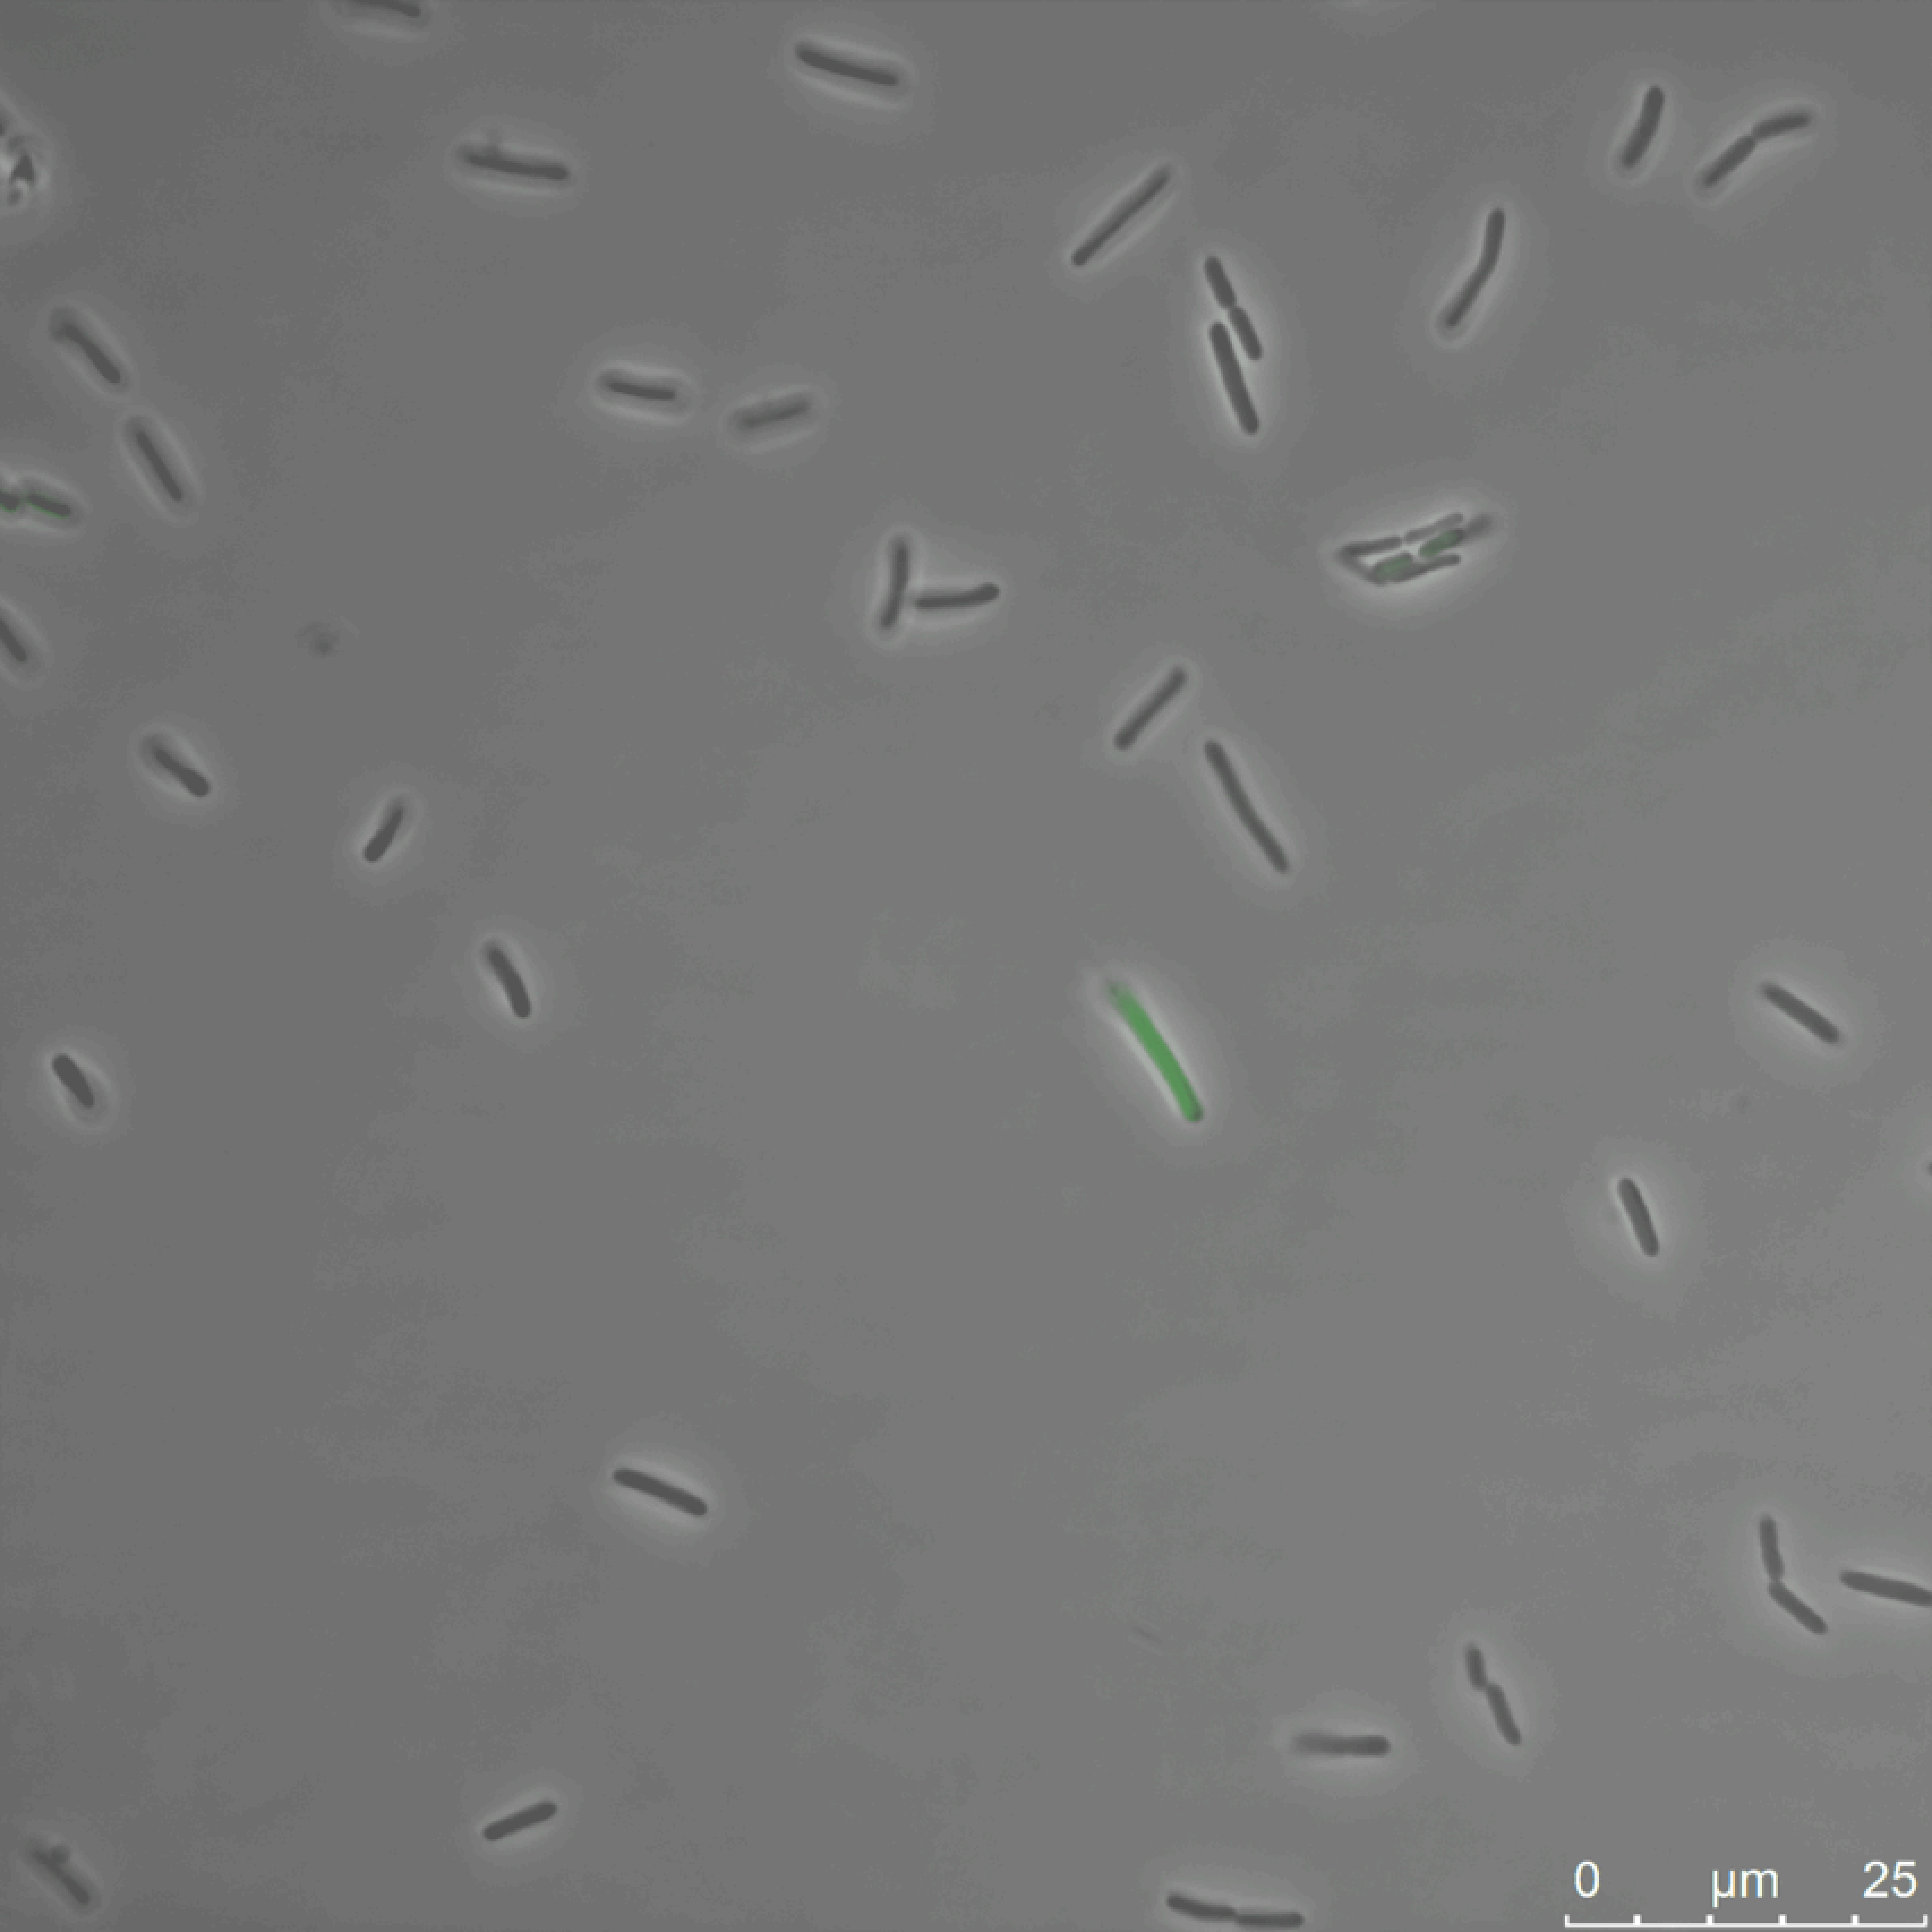
\includegraphics{TT01U4_2_GREEN-crunch-lighter-resample.pdf} &%
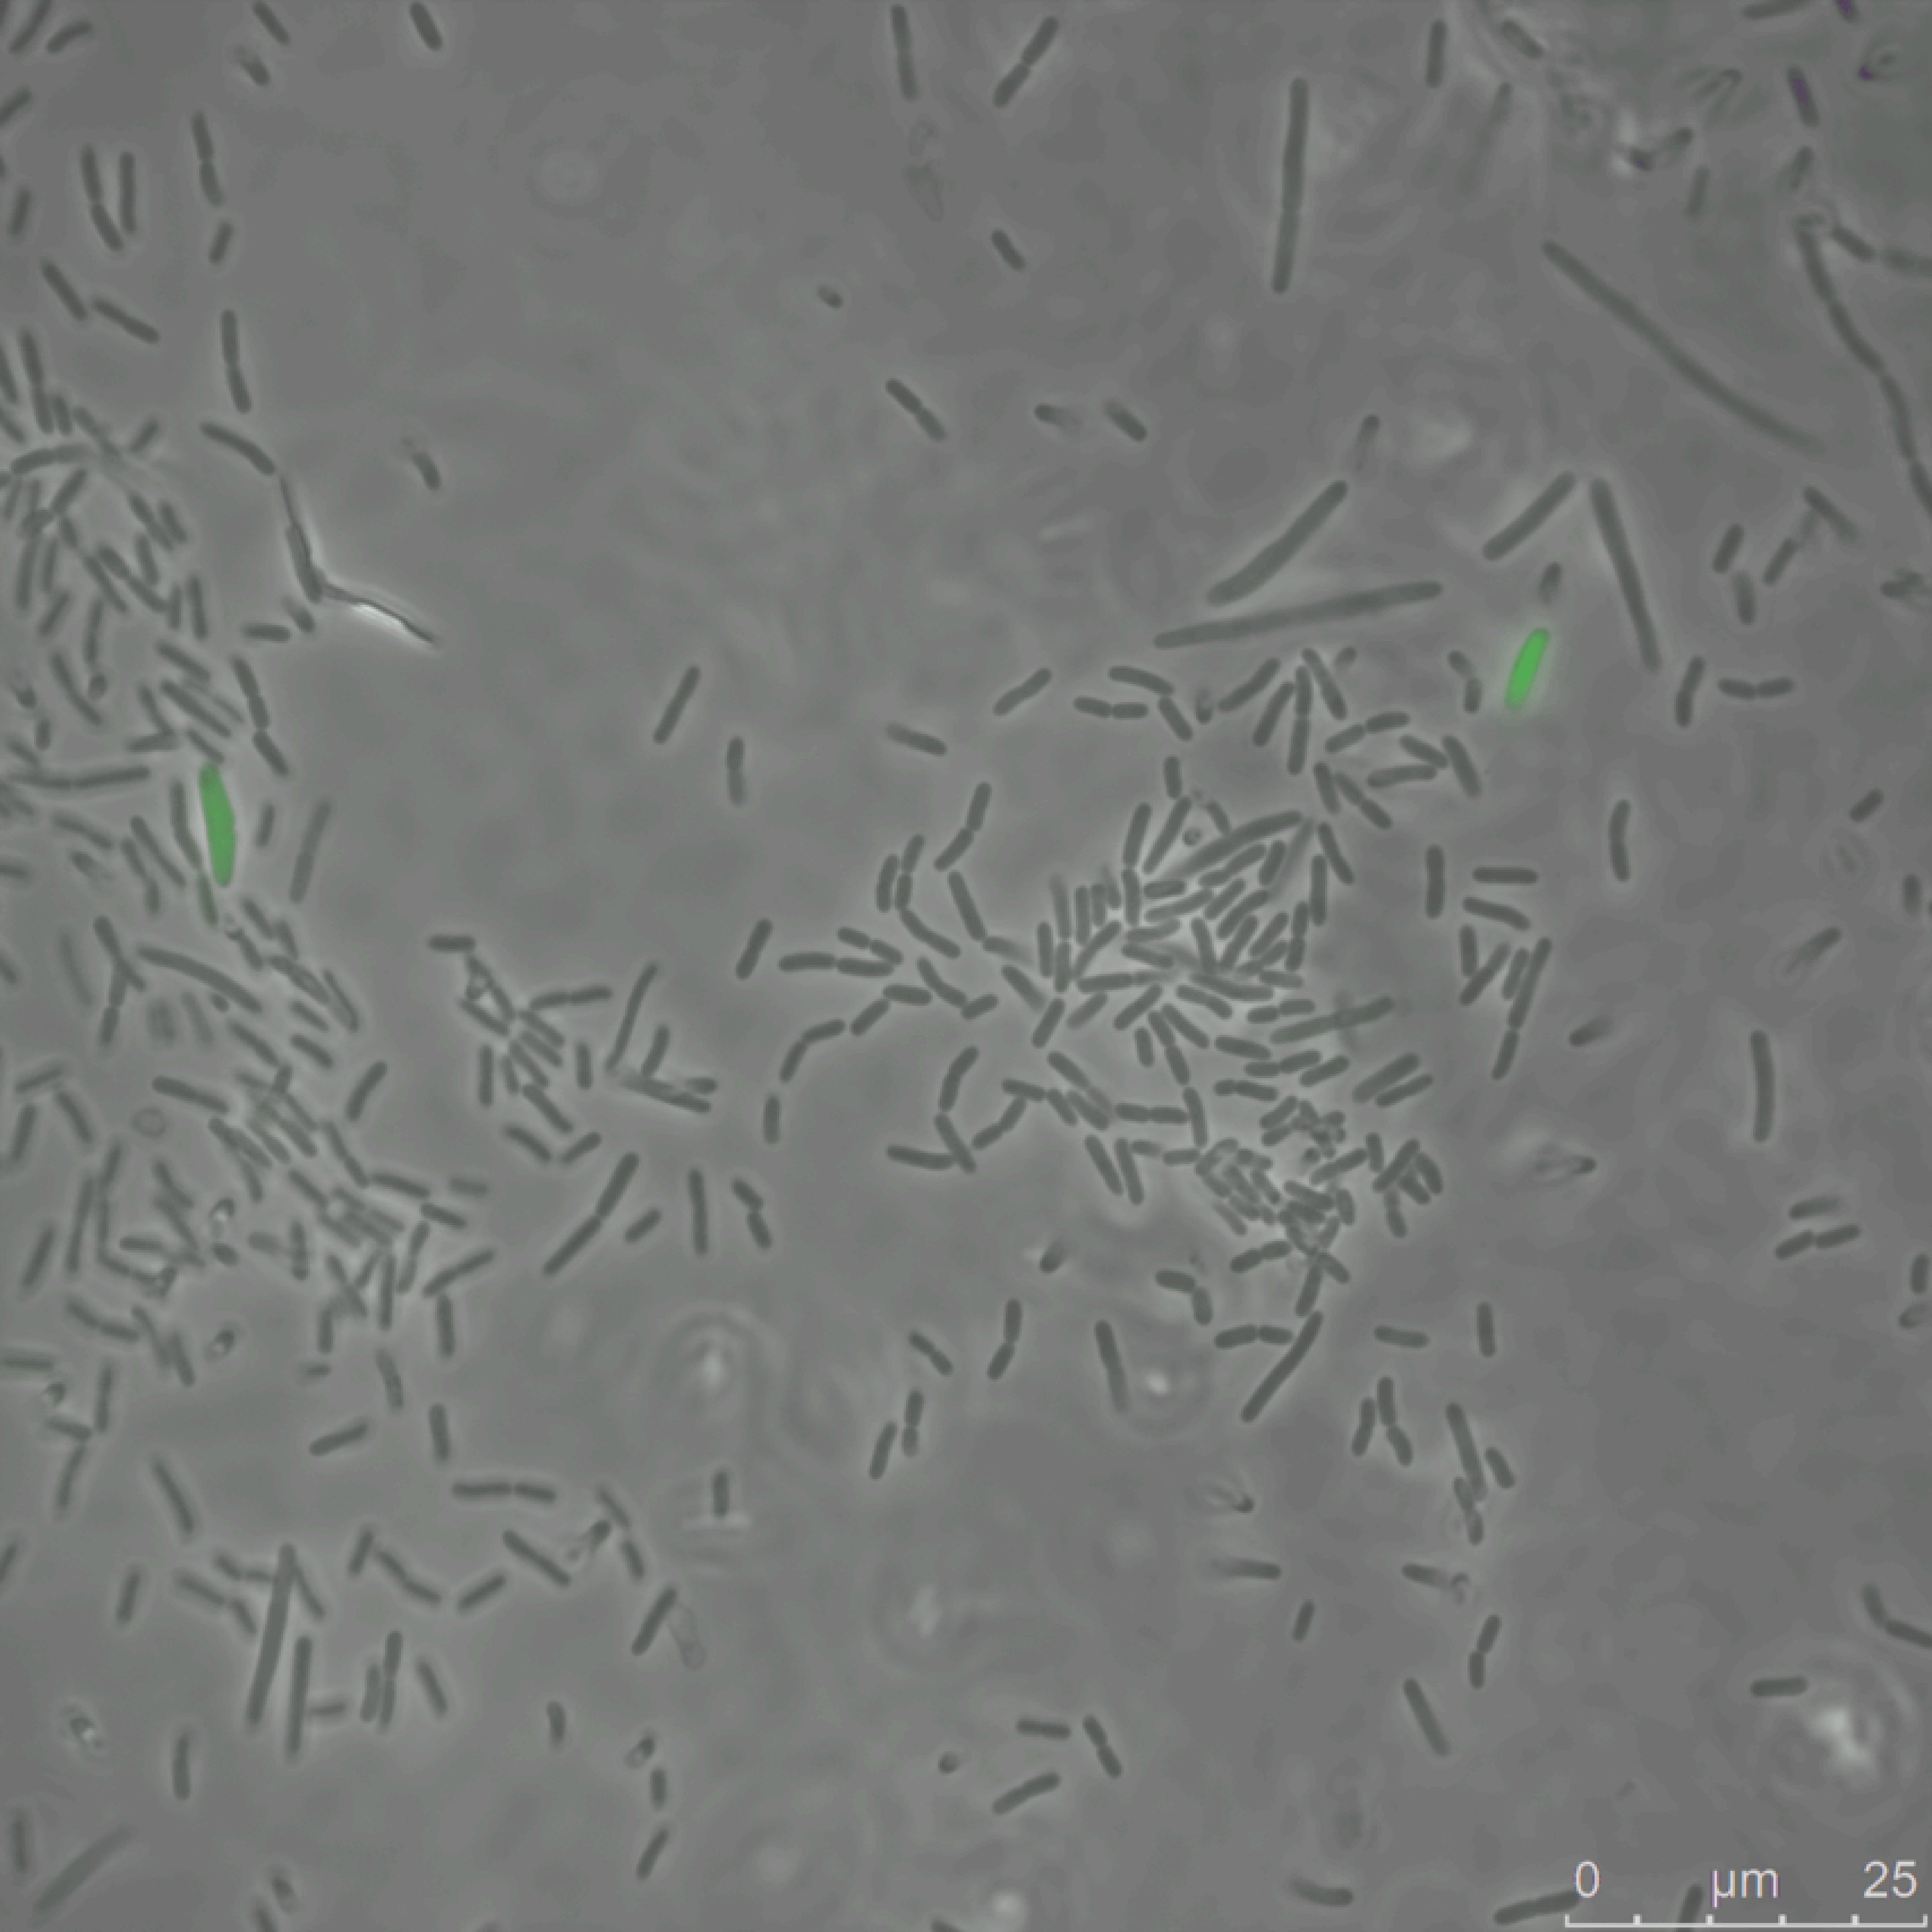
\includegraphics{TT01U4_5HR_2_GREEN-crunch-lighter-resample.pdf} &%
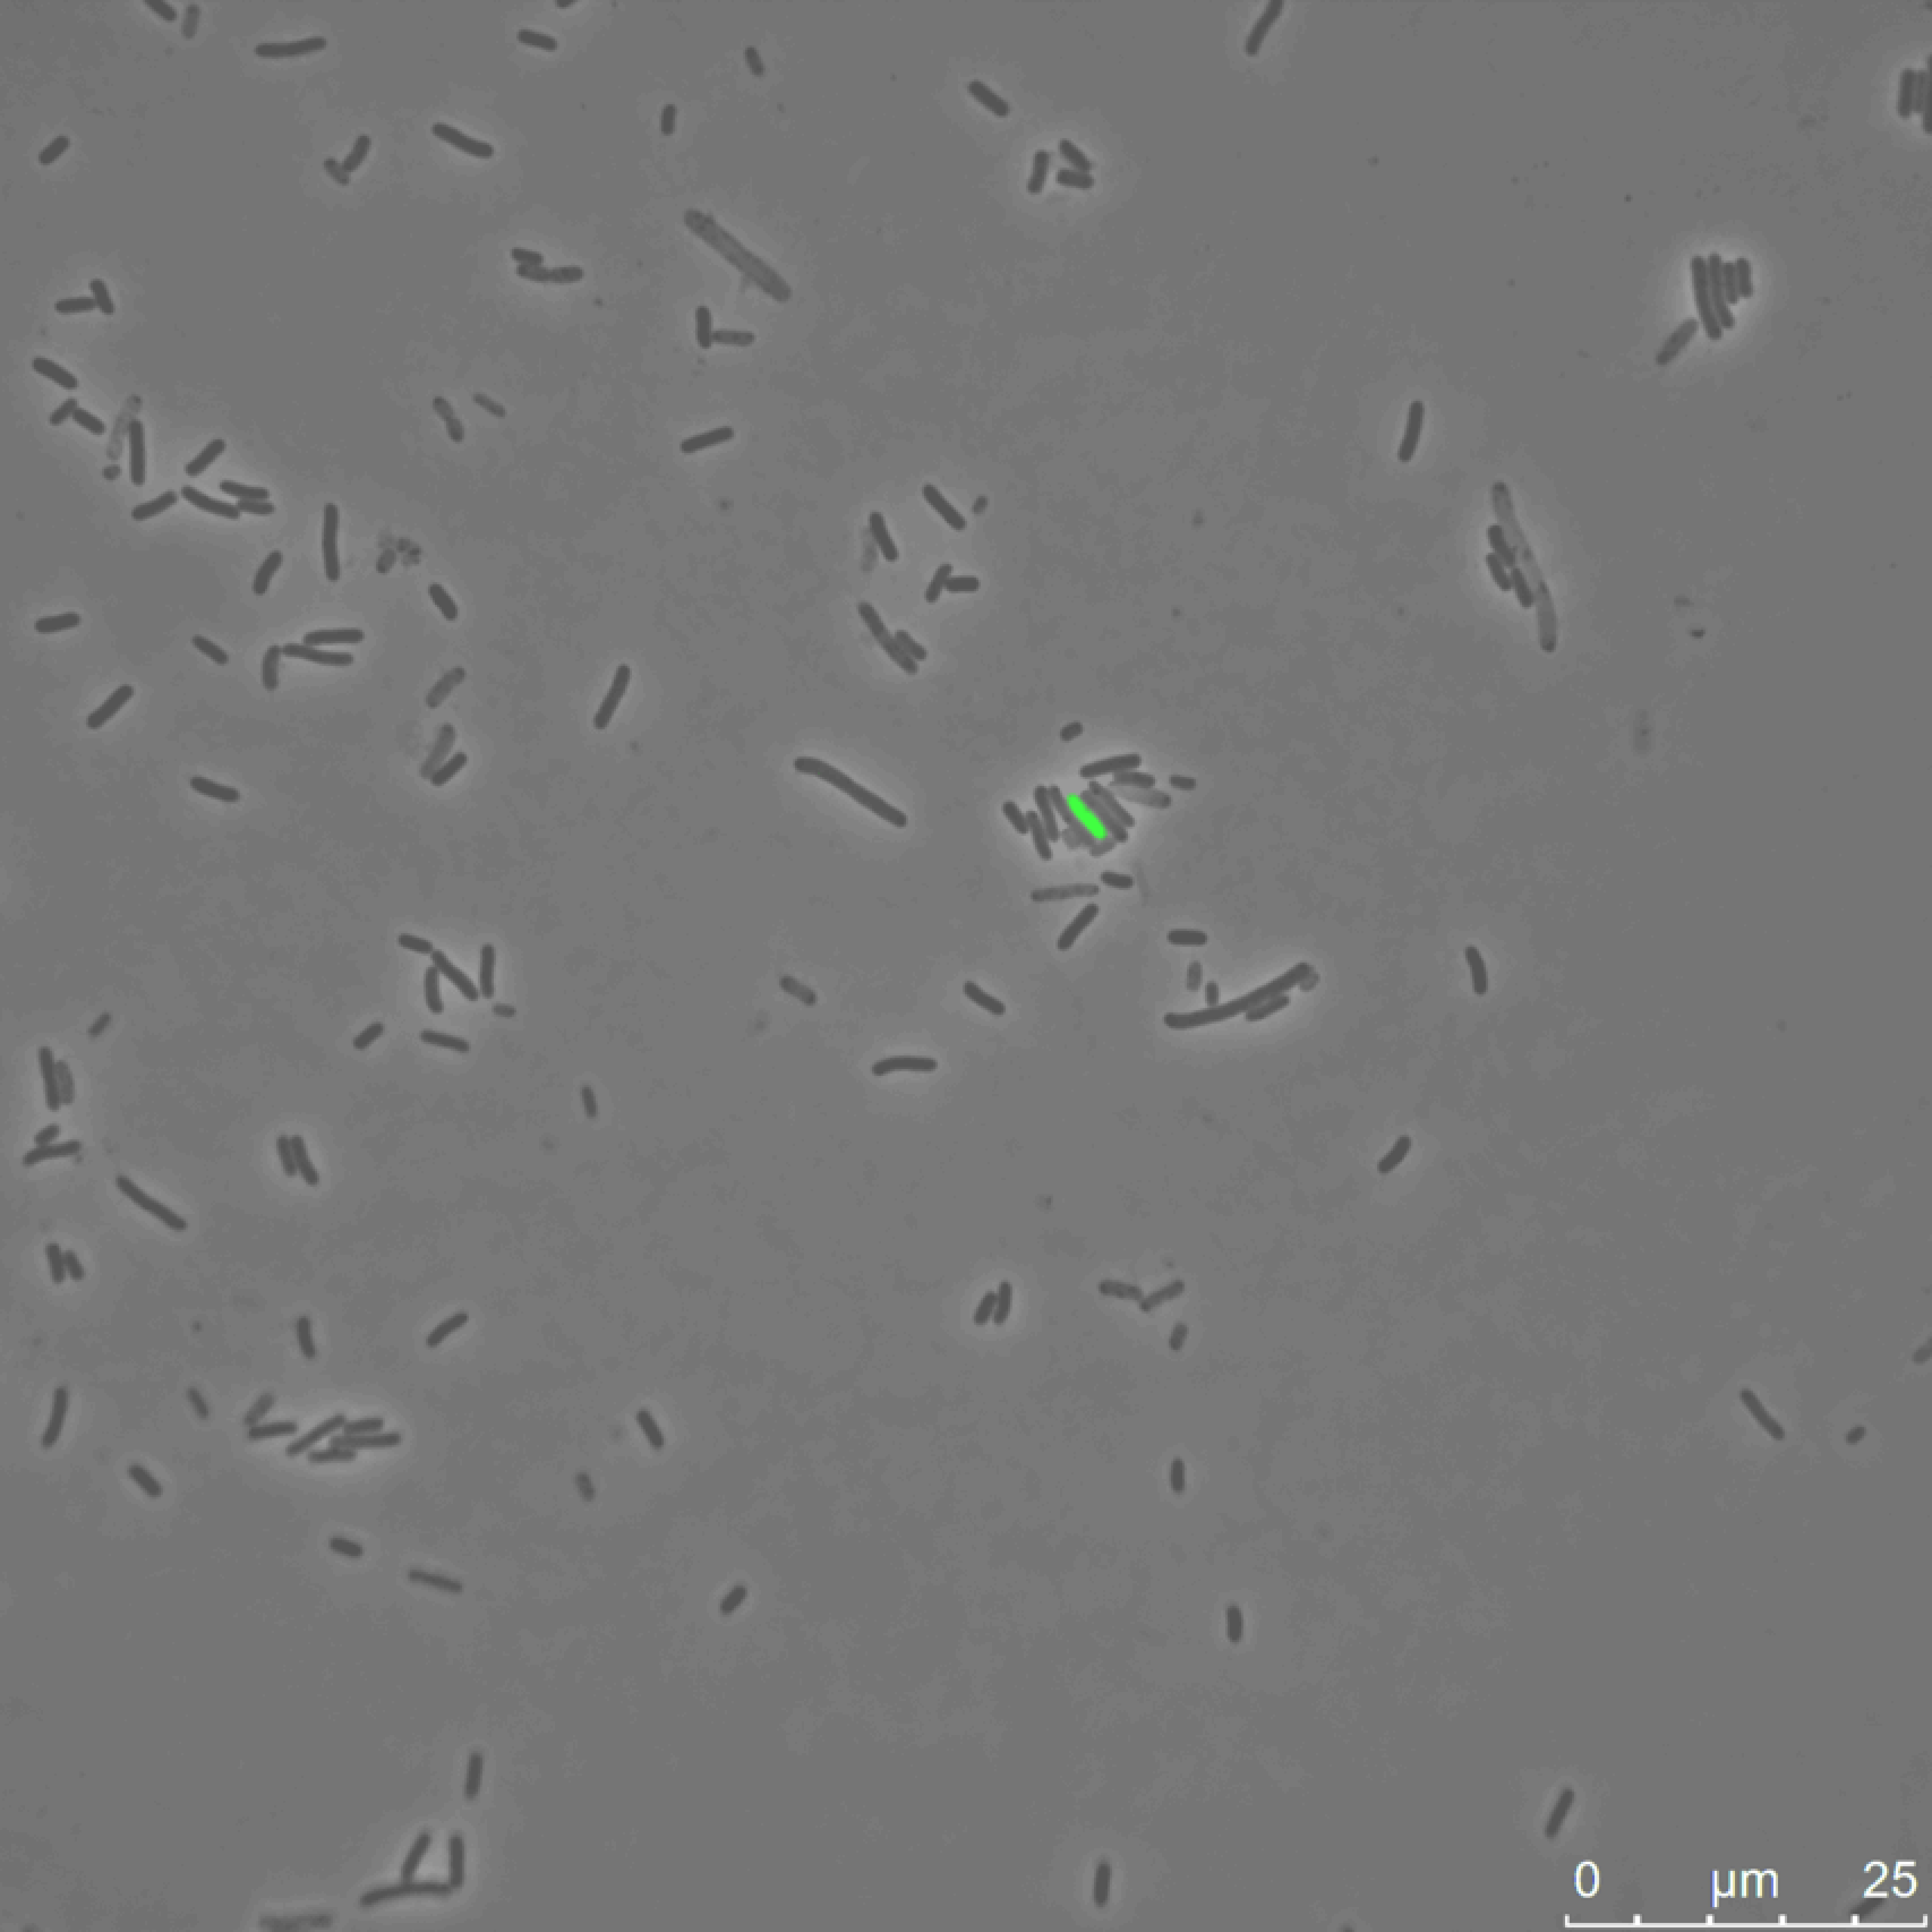
\includegraphics{TT01U4_24HR_2_GREEN-crunch-lighter-resample.pdf} &%
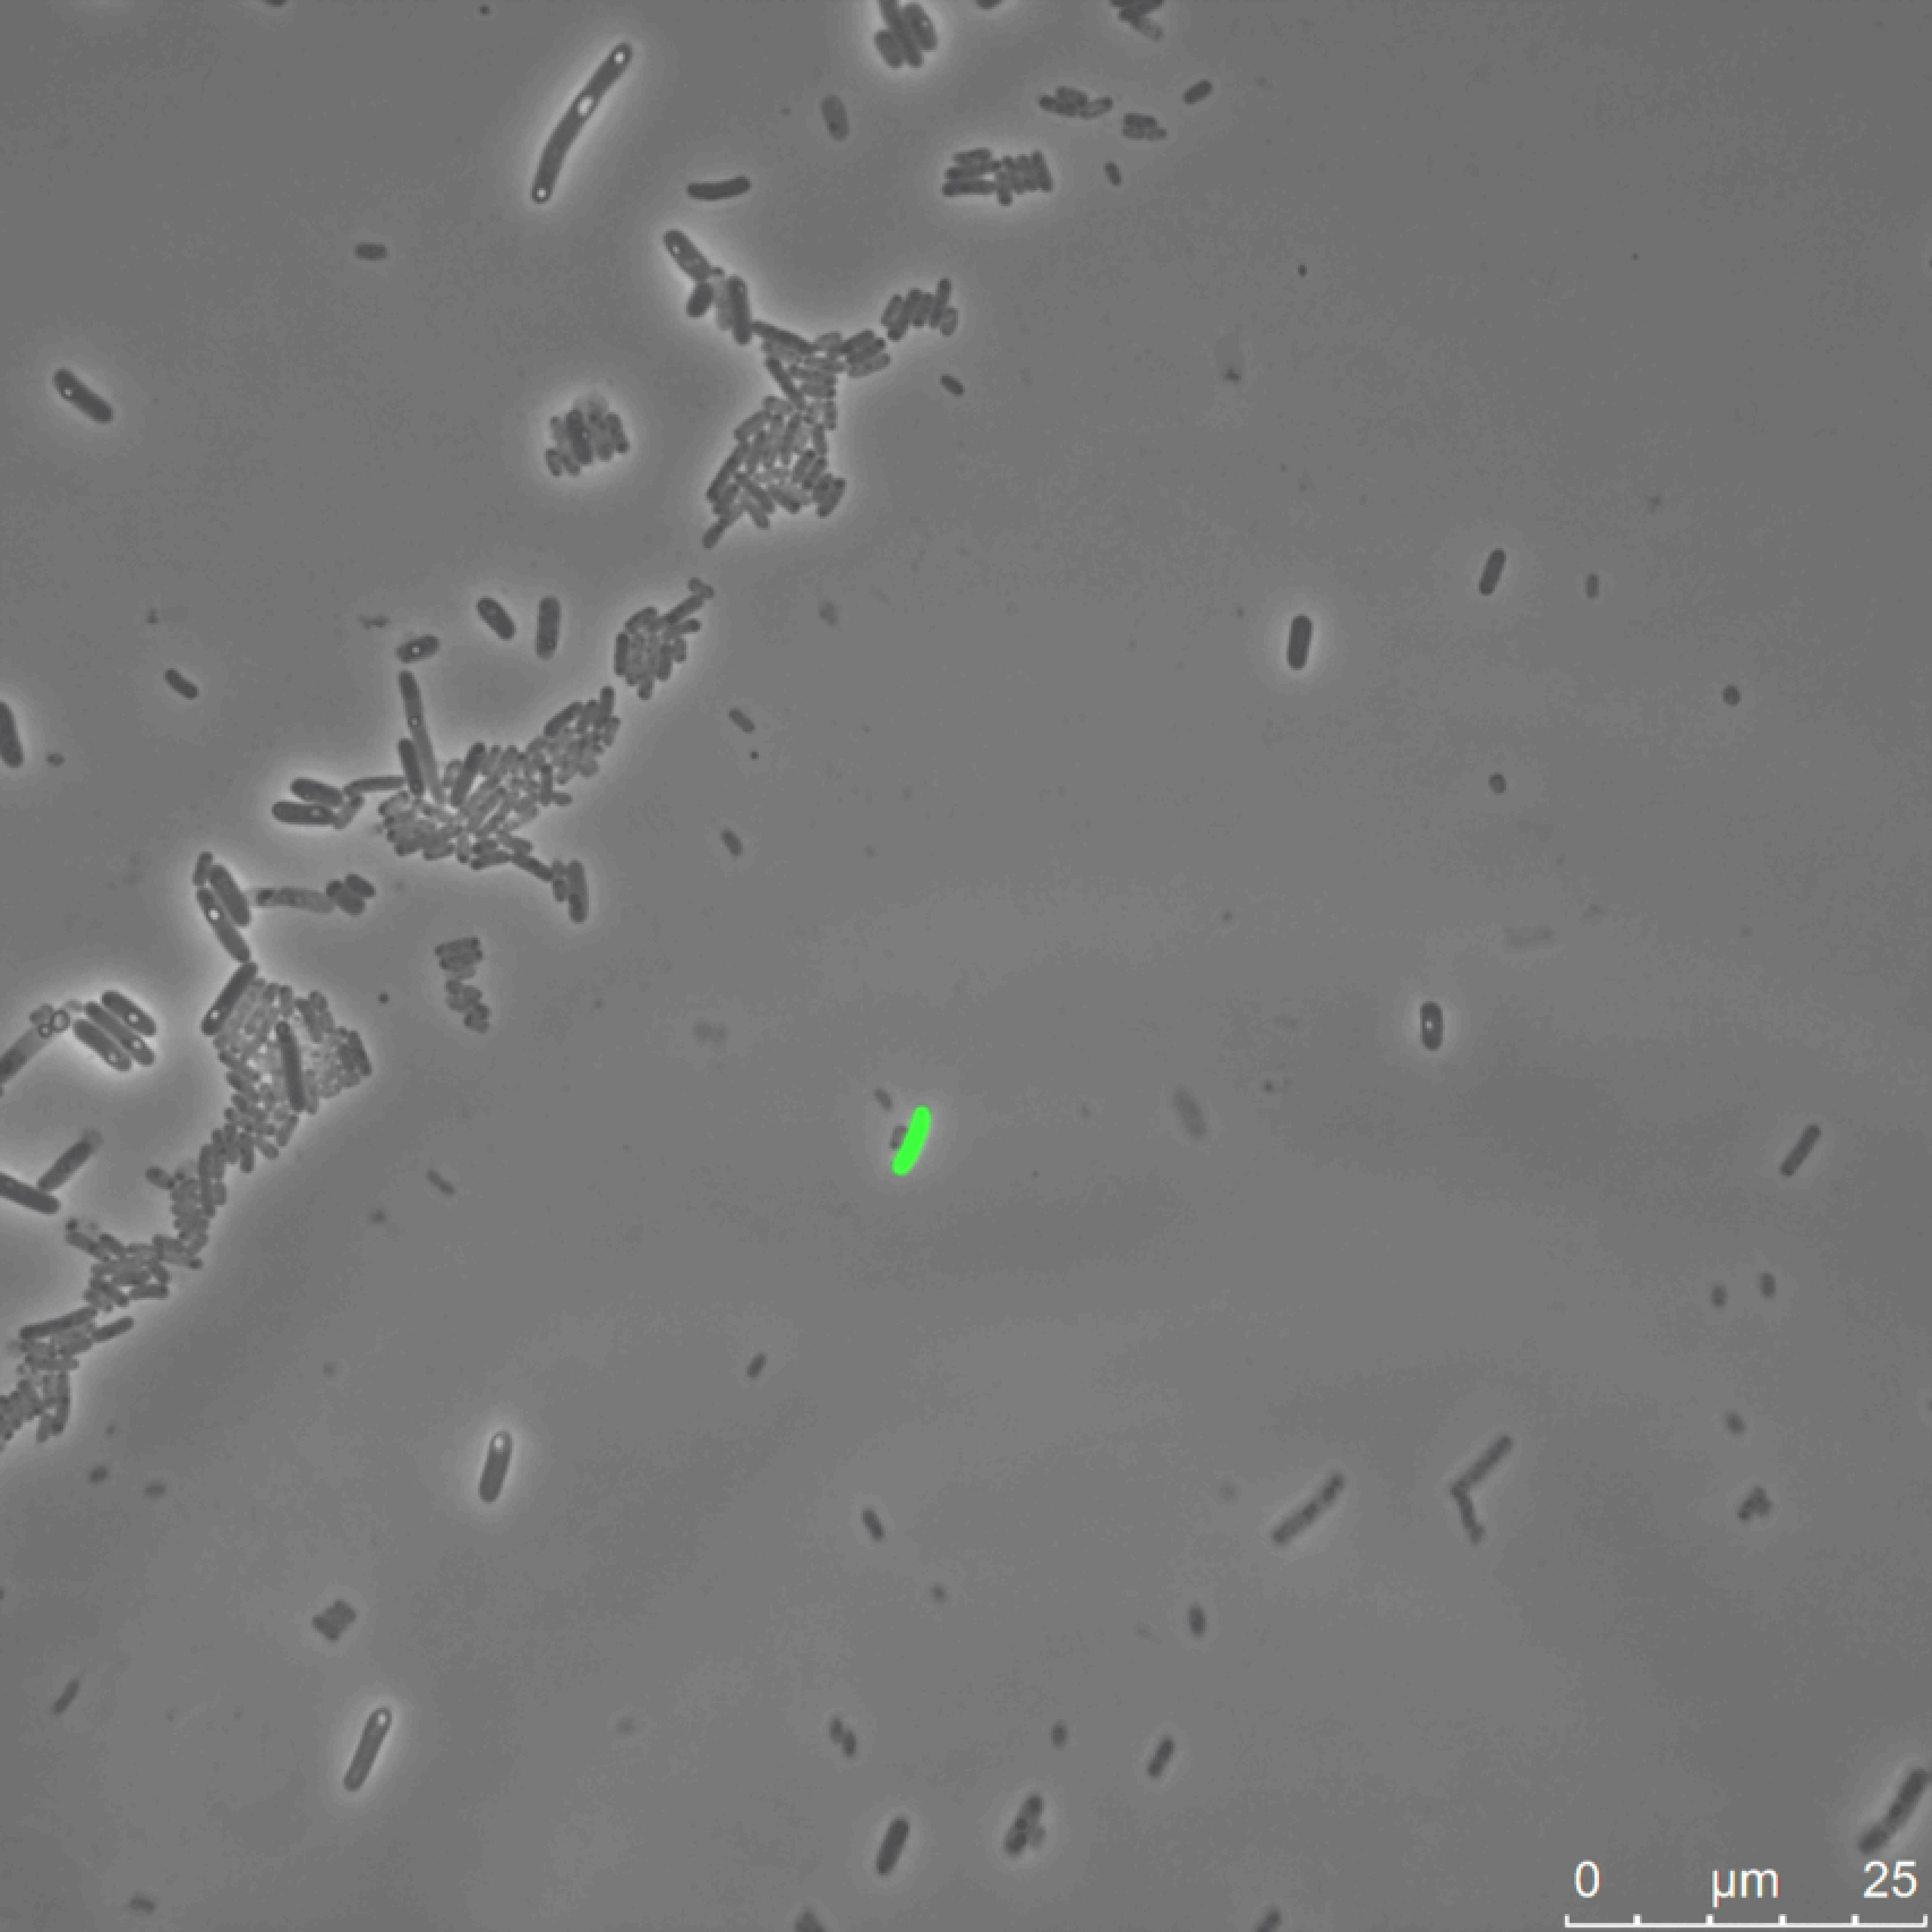
\includegraphics{TT01U4_72HR_2_GREEN-crunch-lighter-resample.pdf} \\[-0.5ex]

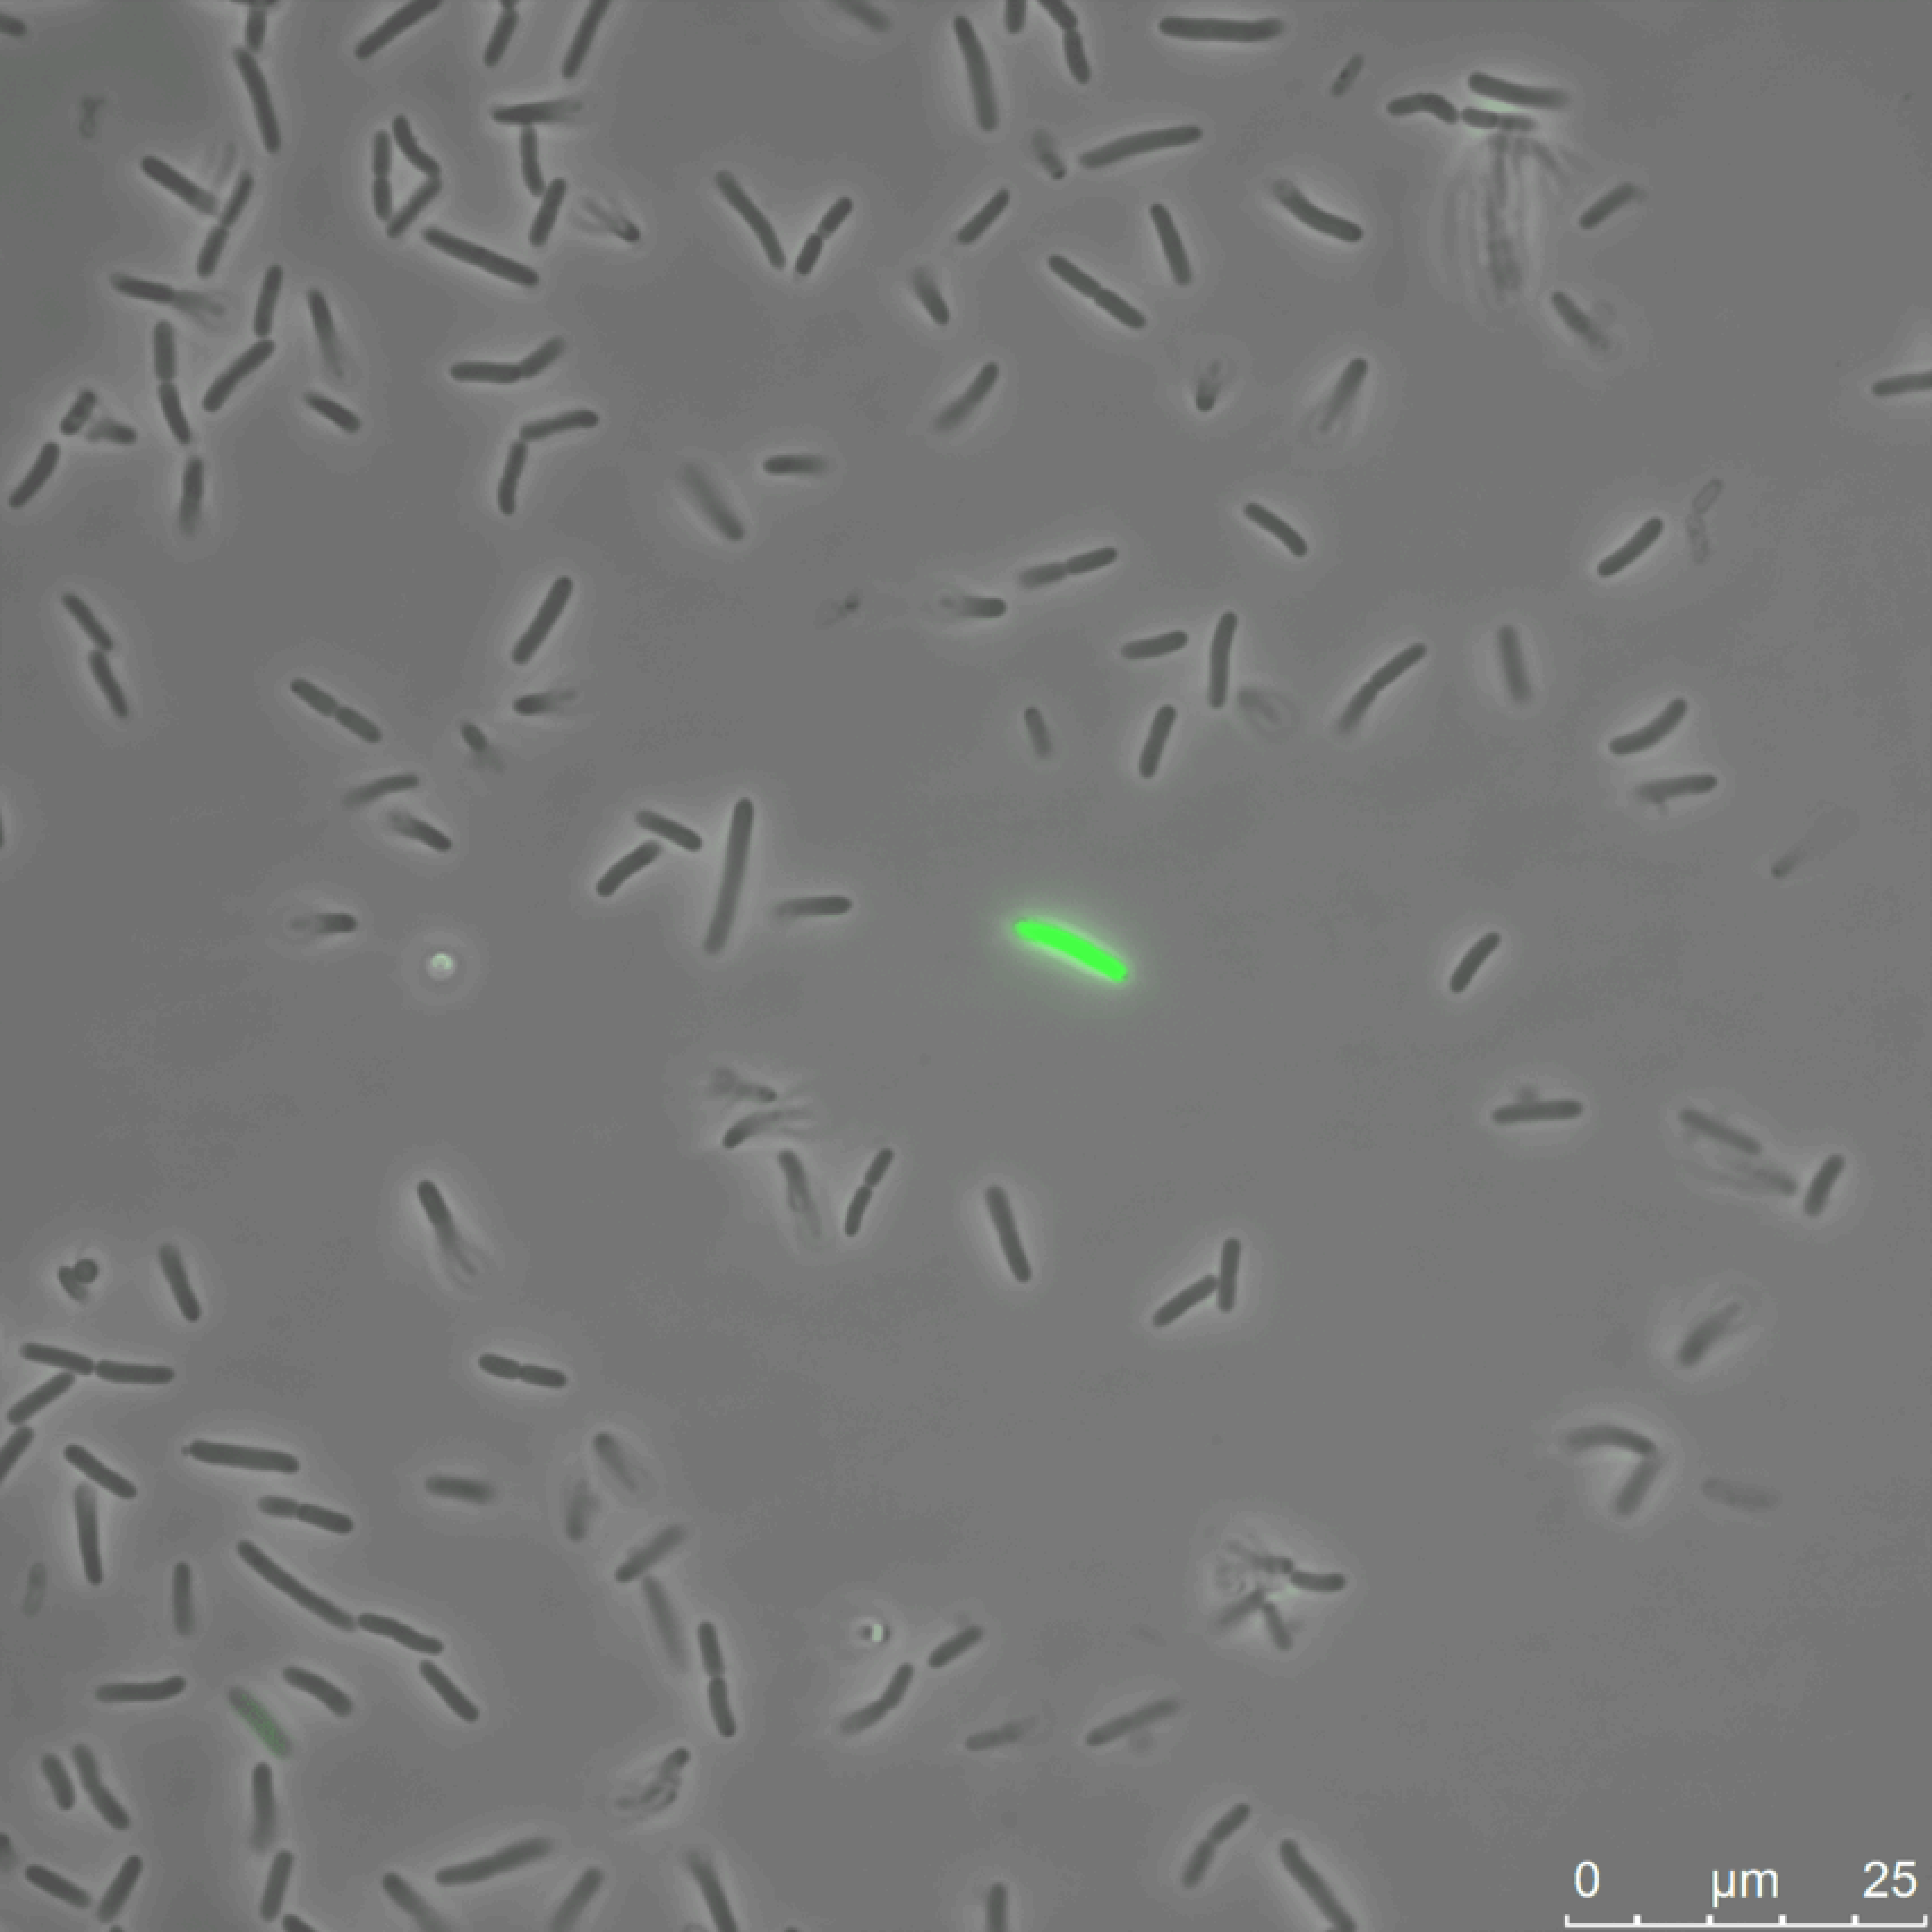
\includegraphics{TT01U4_5_GREEN-crunch-lighter-resample.pdf} &%
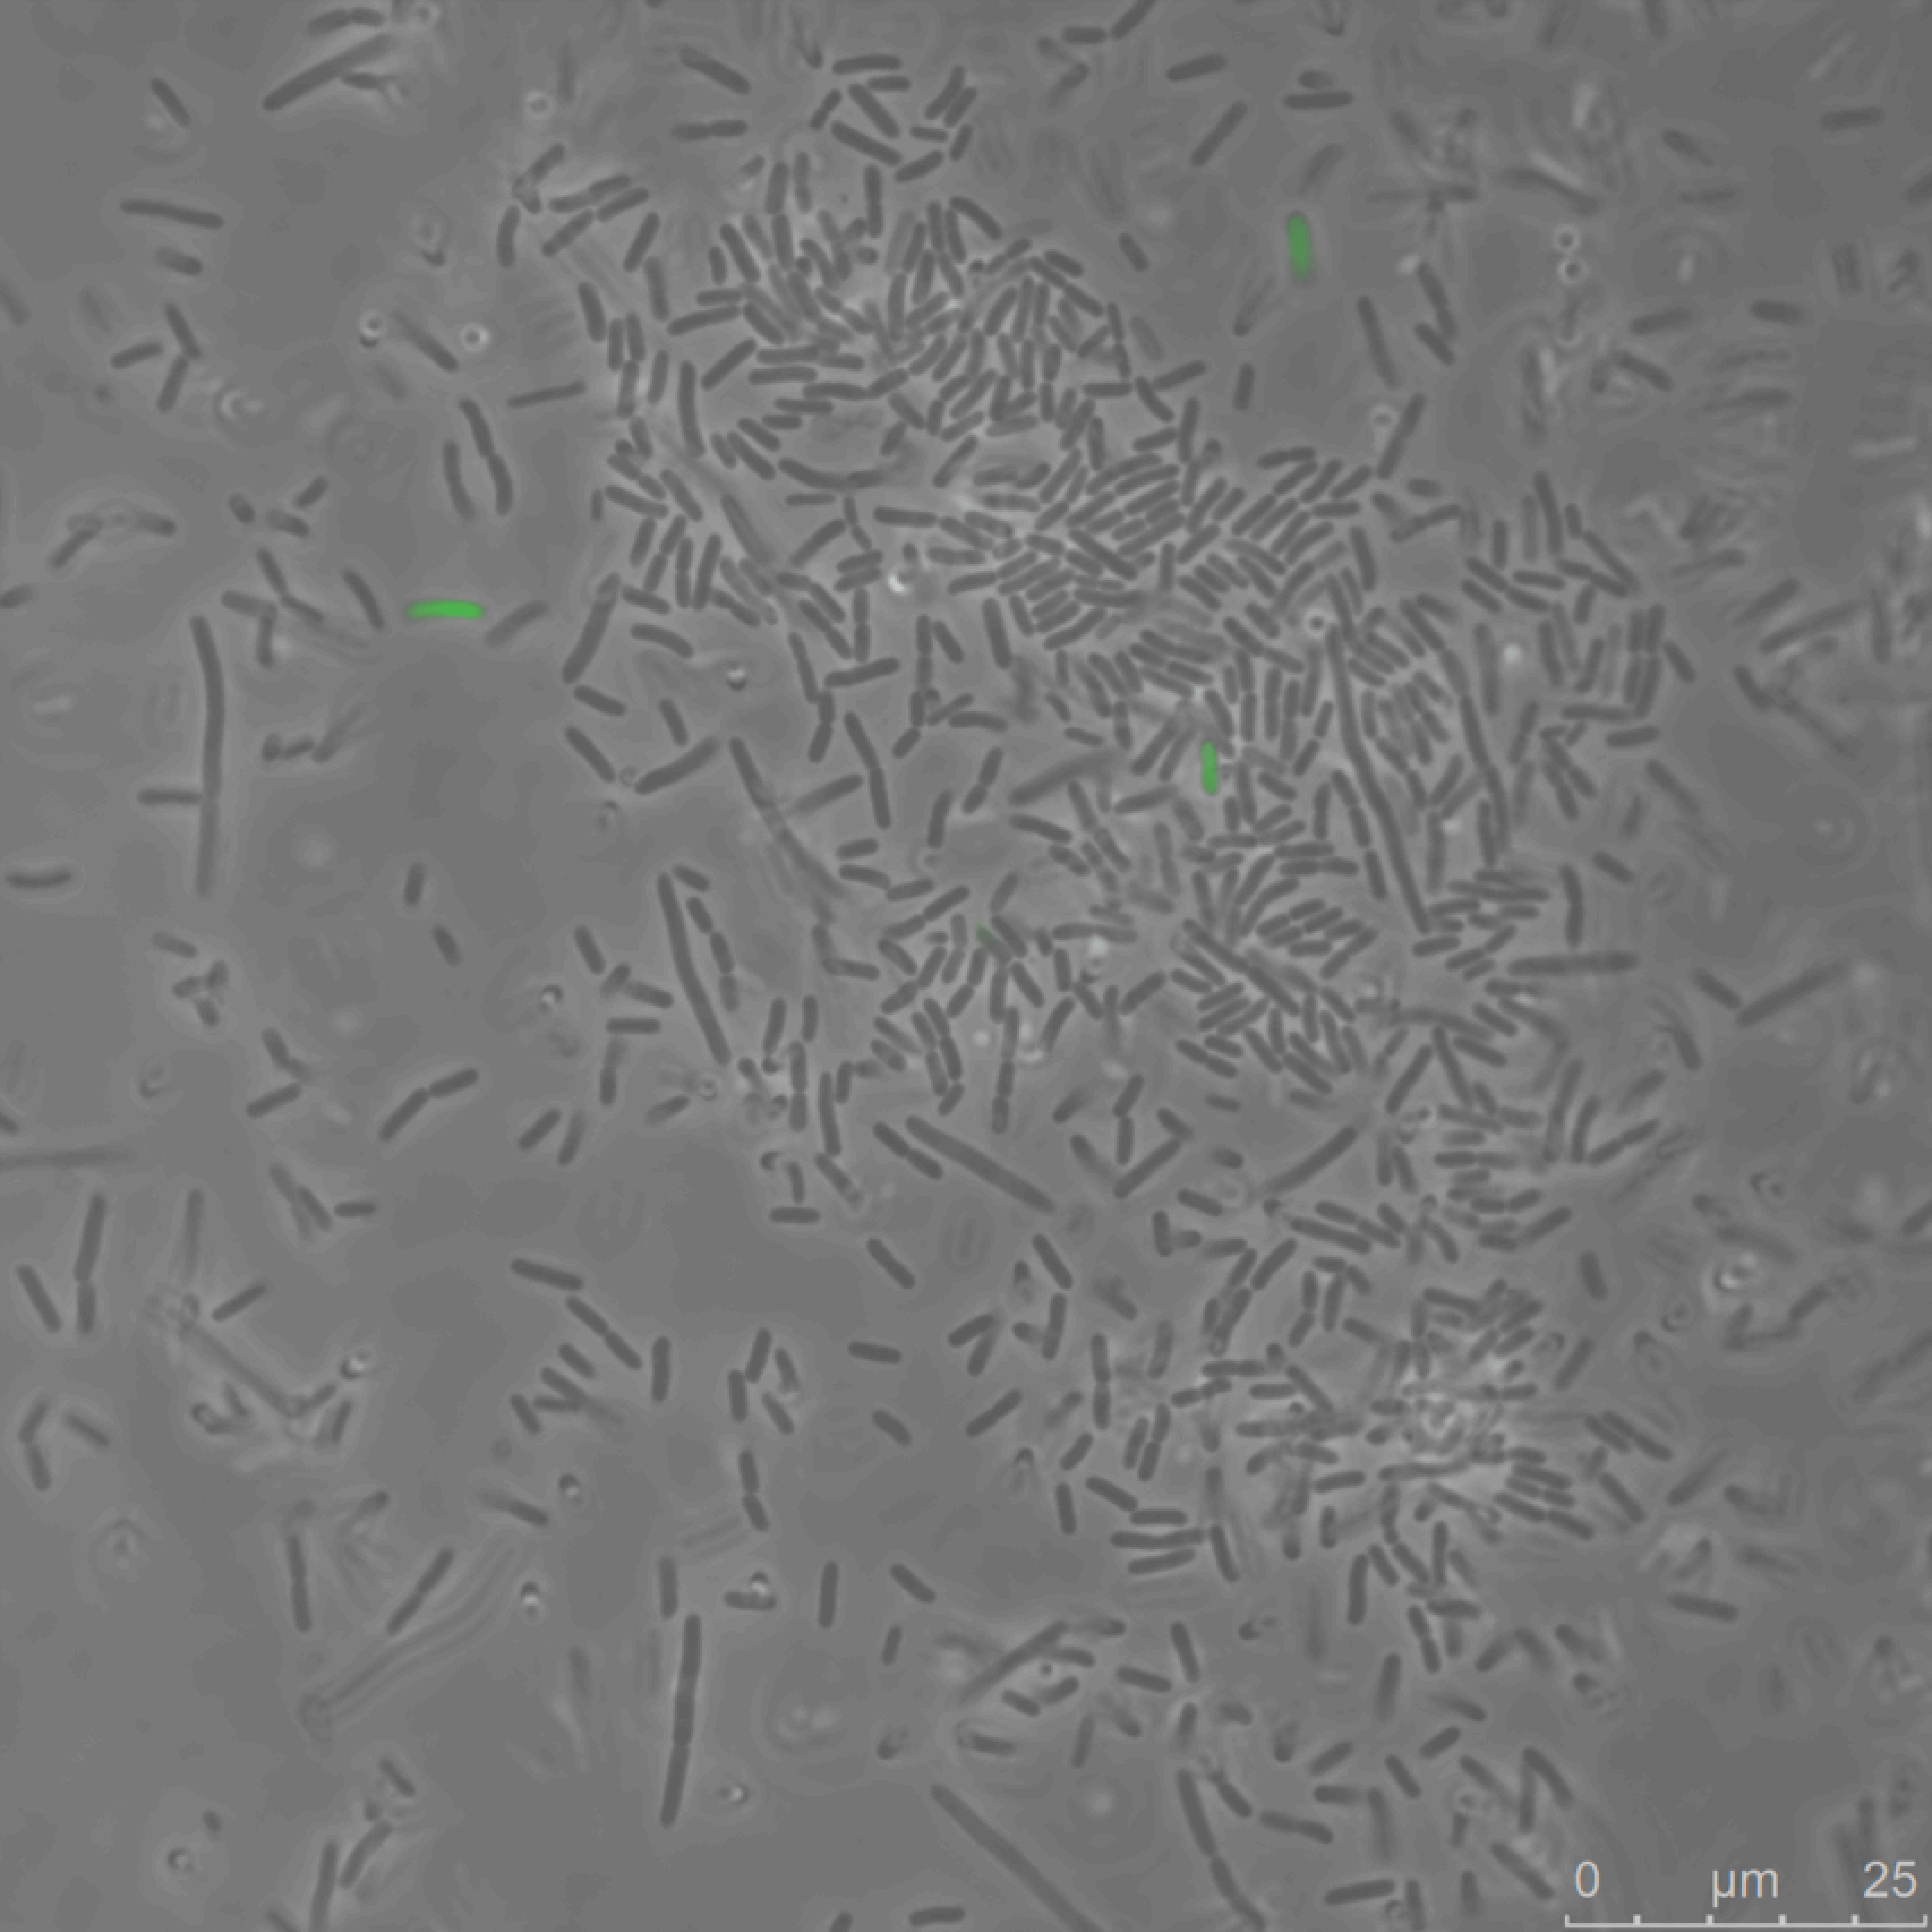
\includegraphics{TT01U4_5HR_3_GREEN-crunch-lighter-resample.pdf} &%
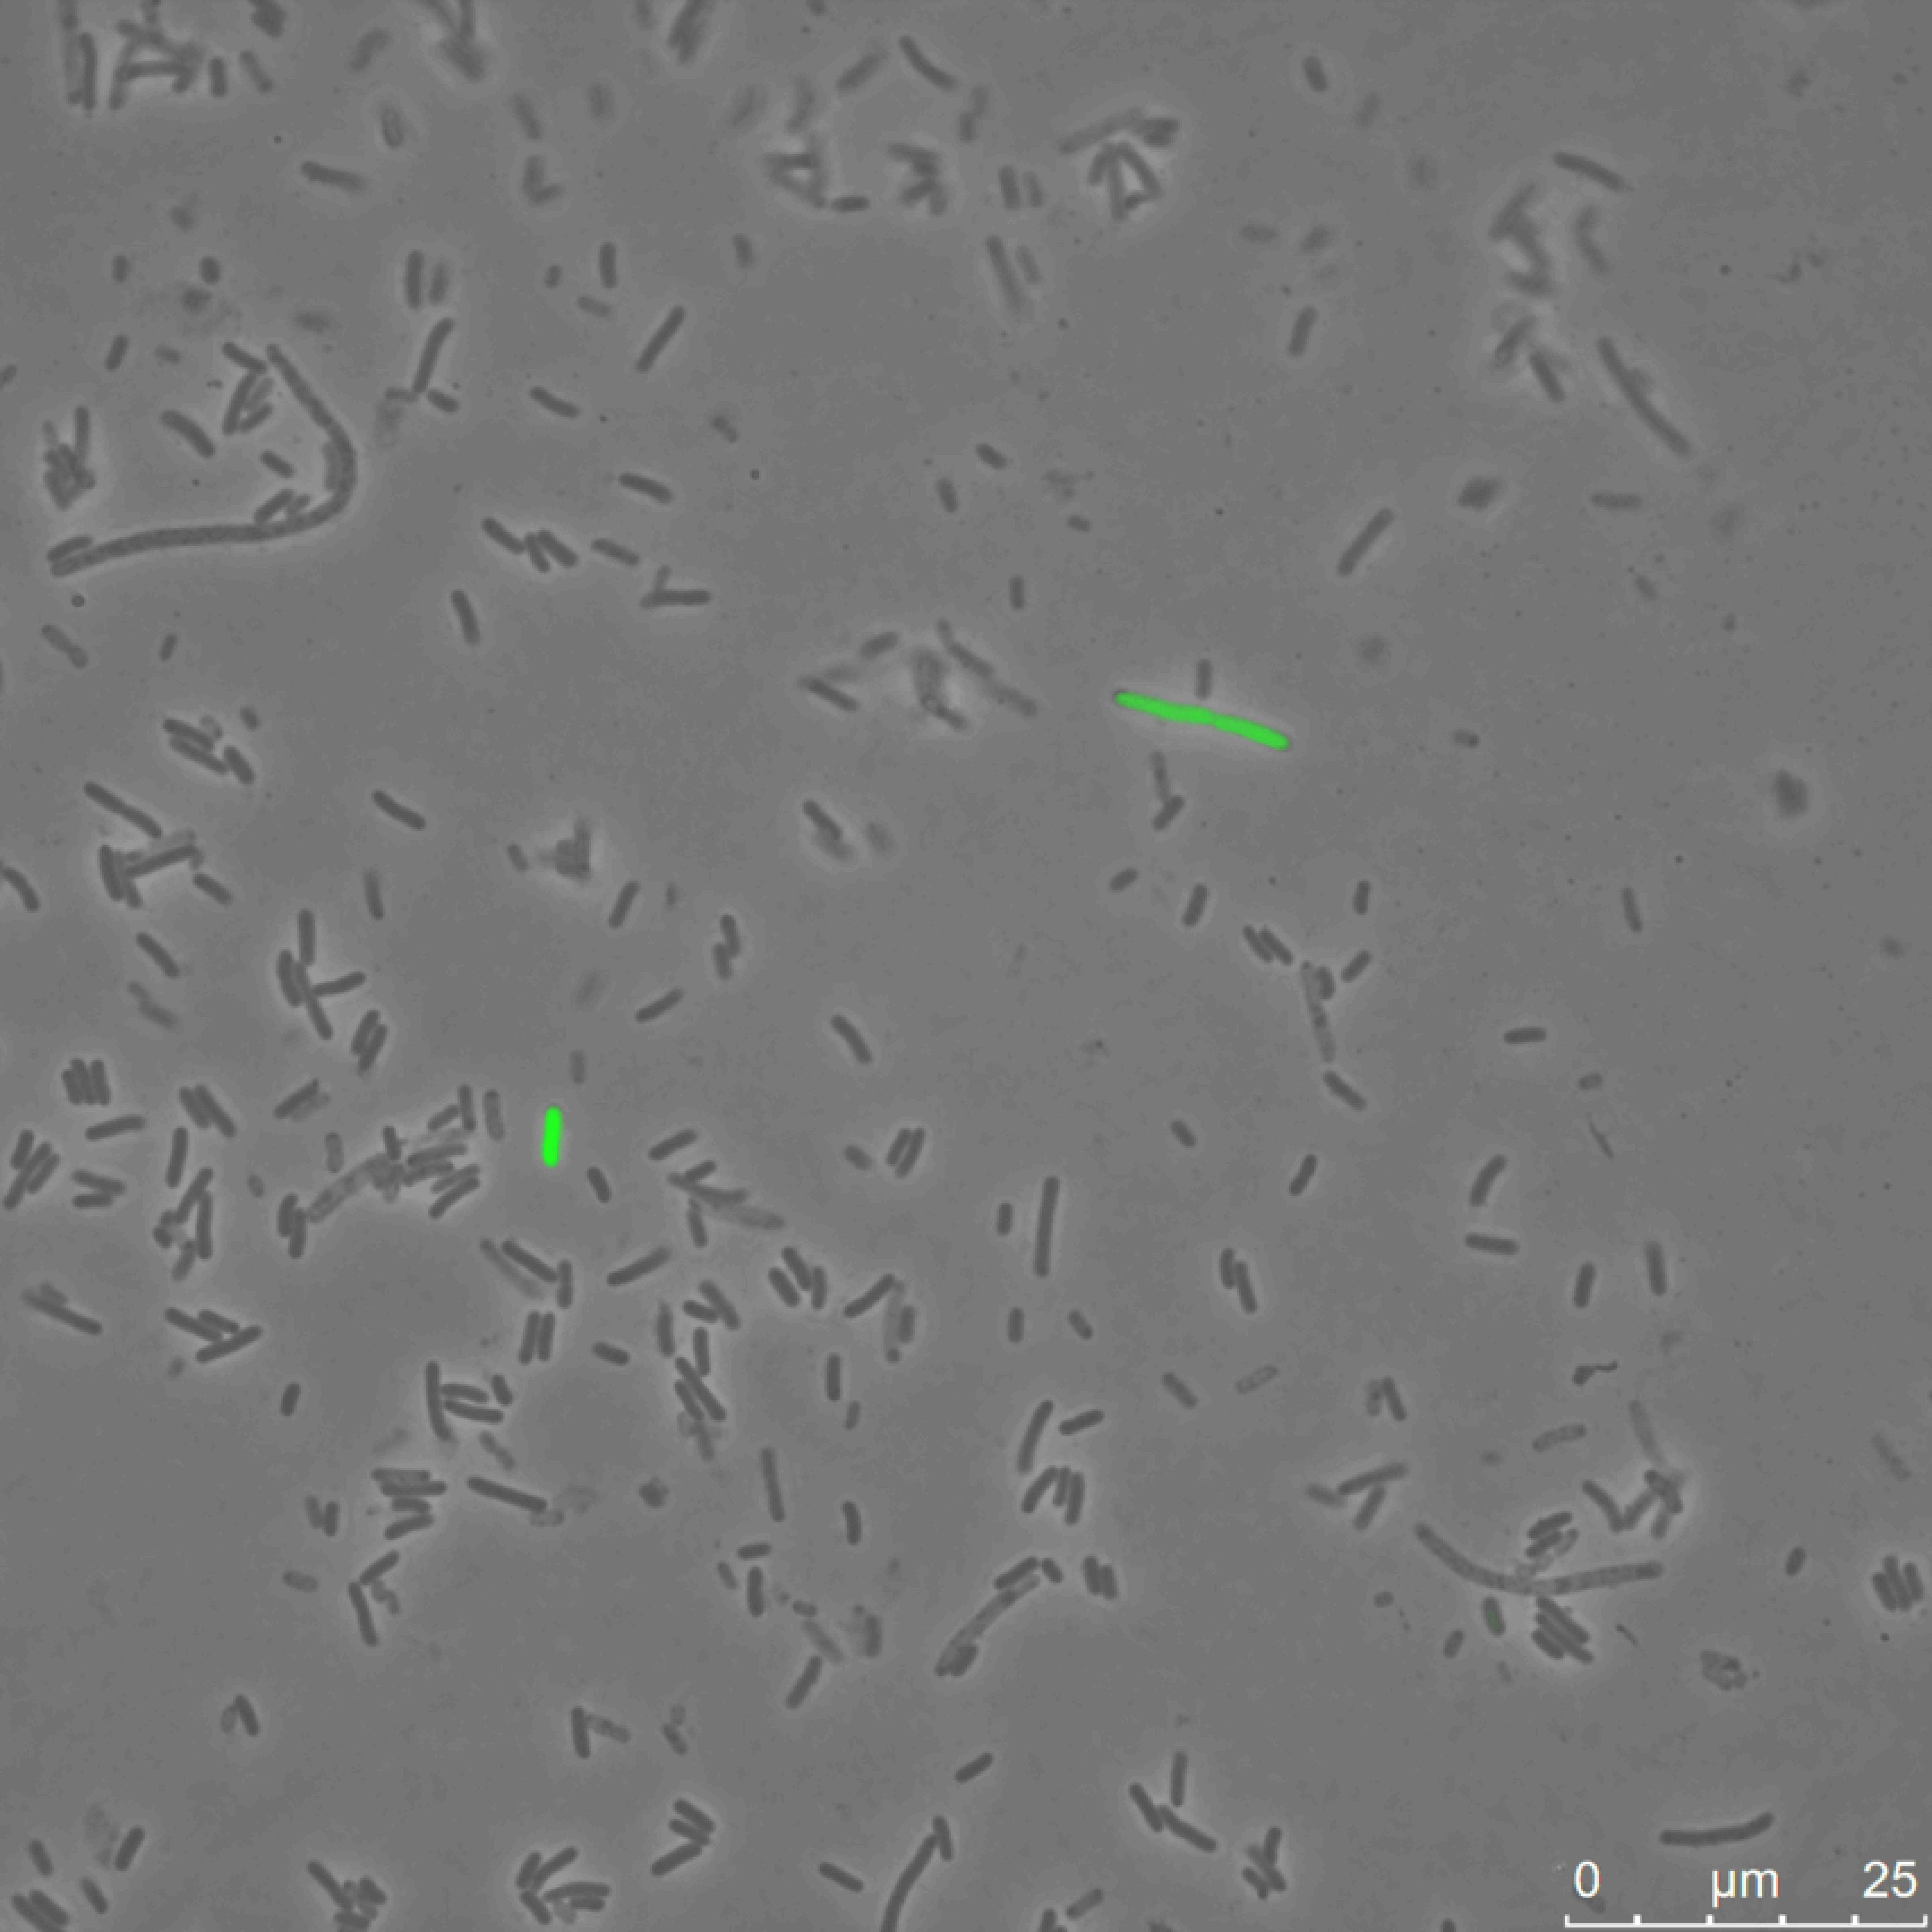
\includegraphics{TT01U4_24HR_3_GREEN-crunch-lighter-resample.pdf} &%
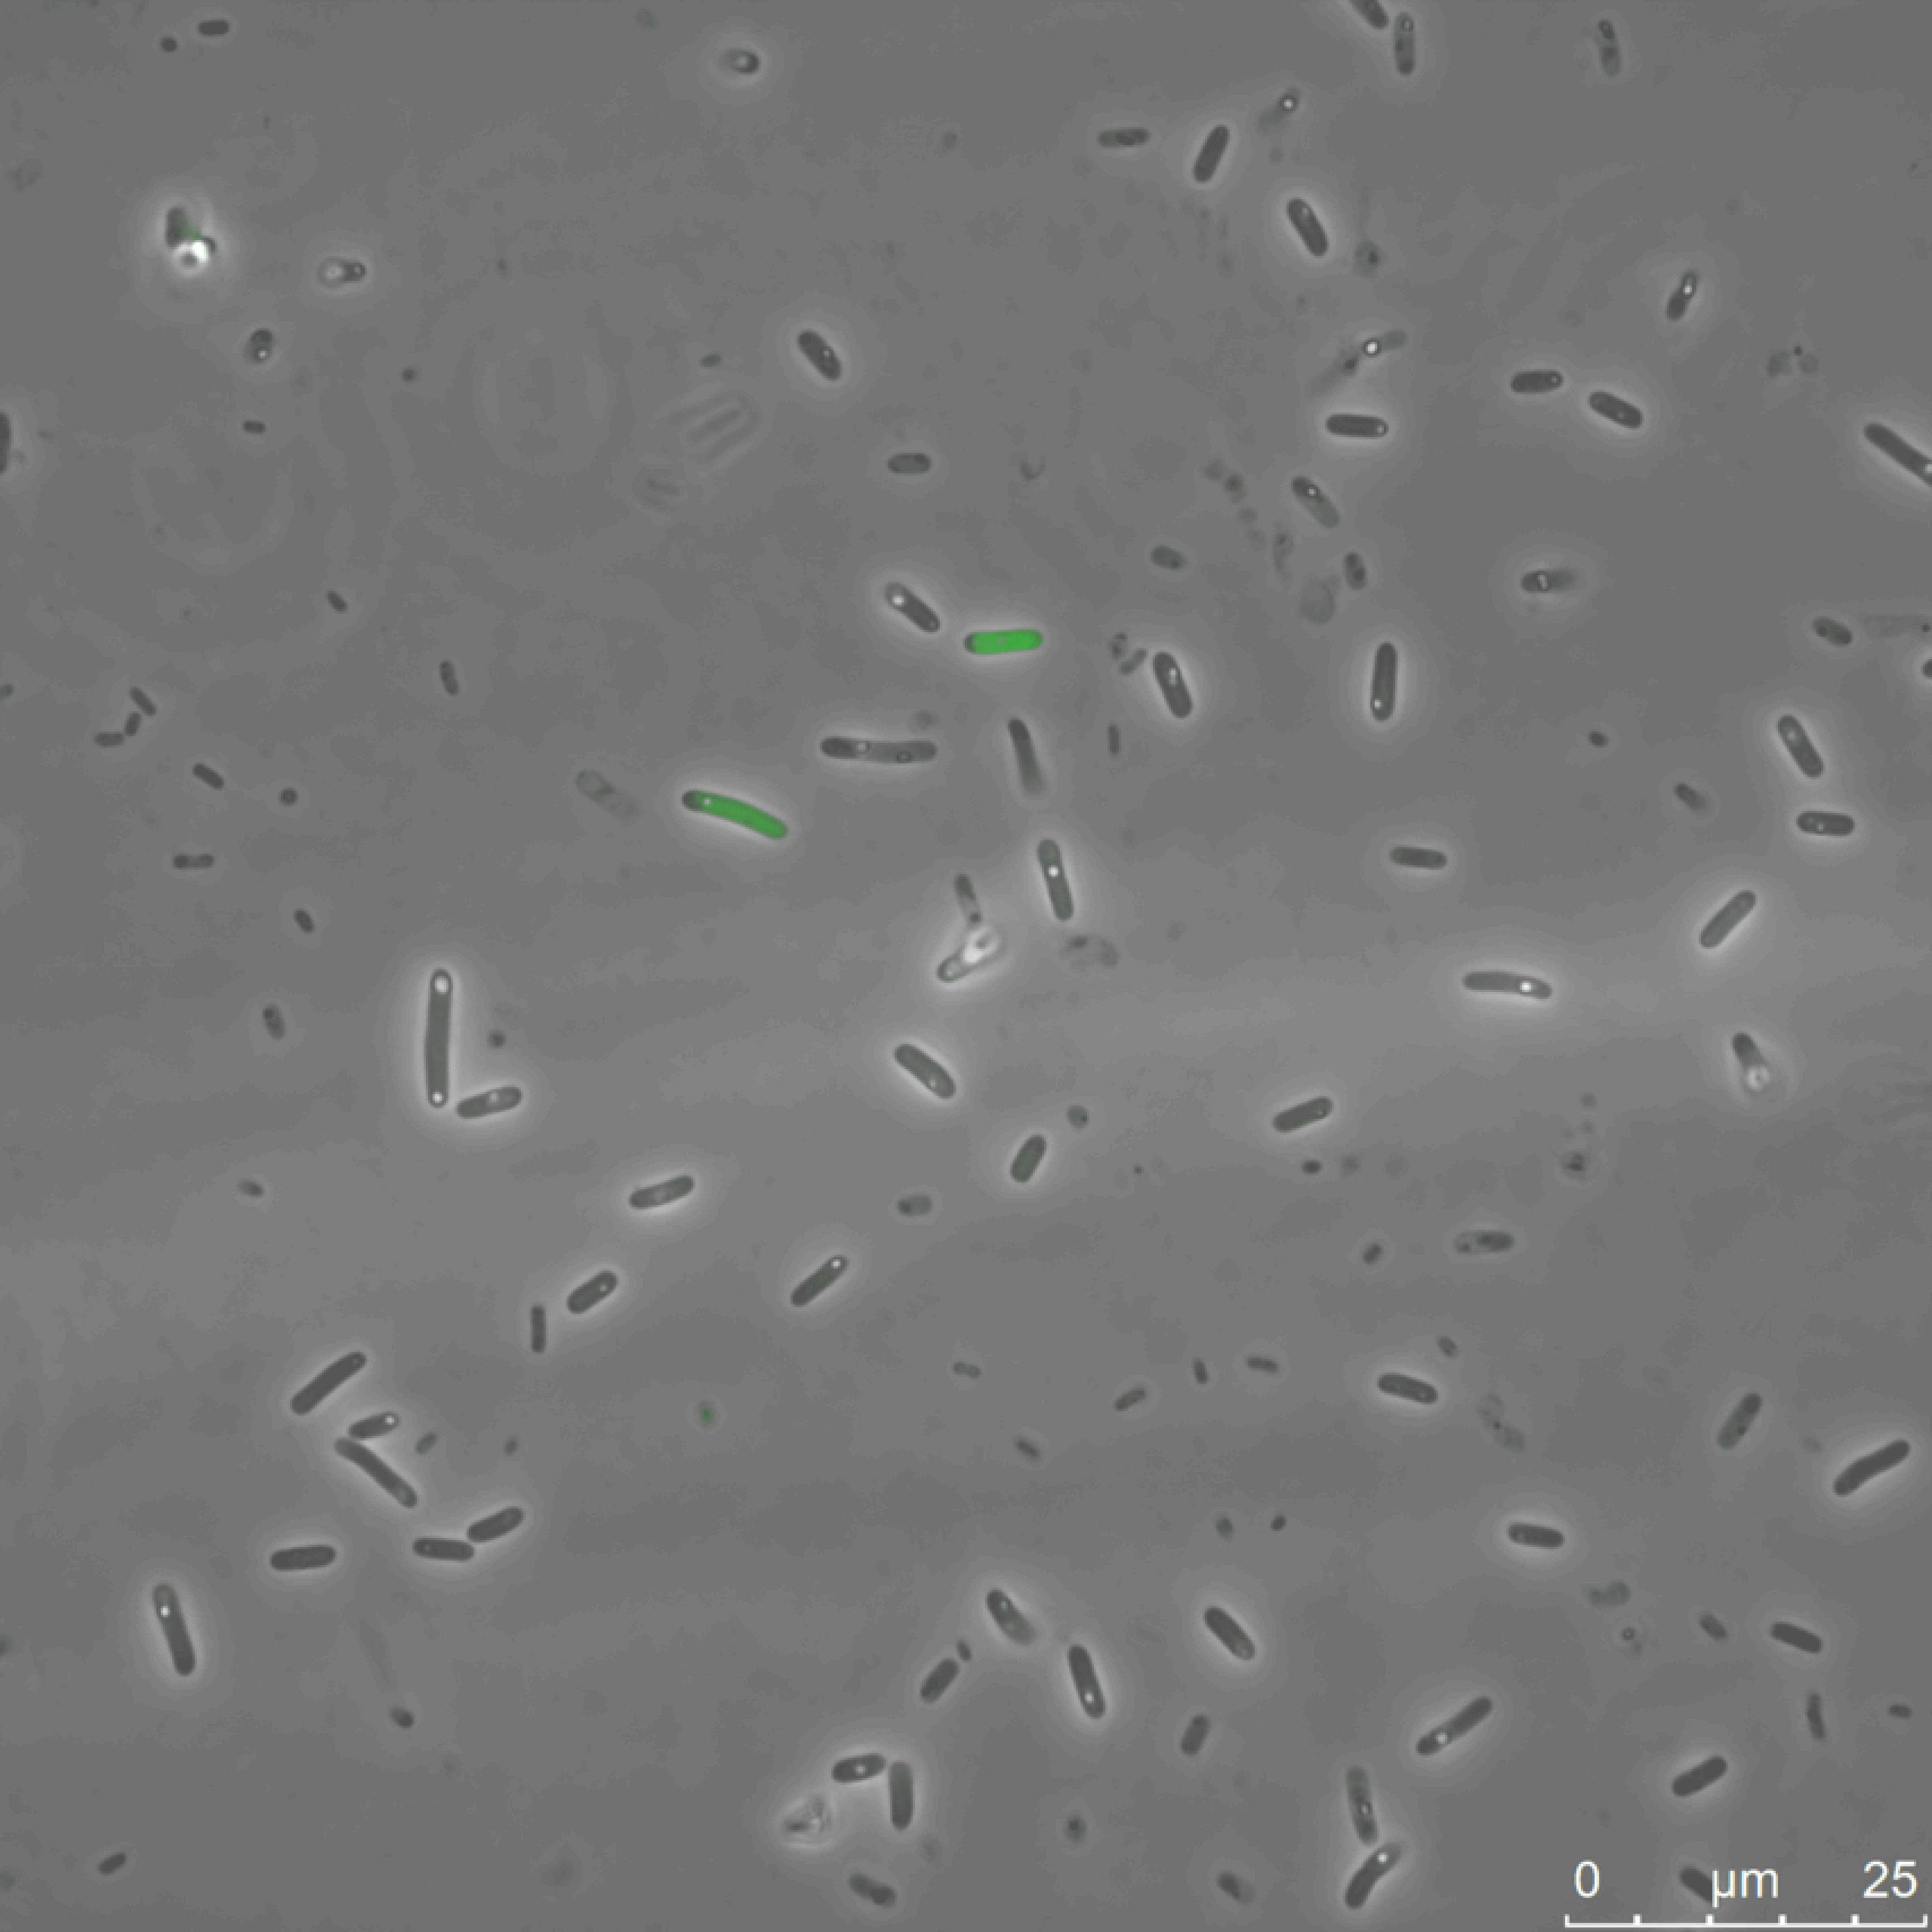
\includegraphics{TT01U4_72HR_3_GREEN-crunch-lighter-resample.pdf} \\[-0.5ex]

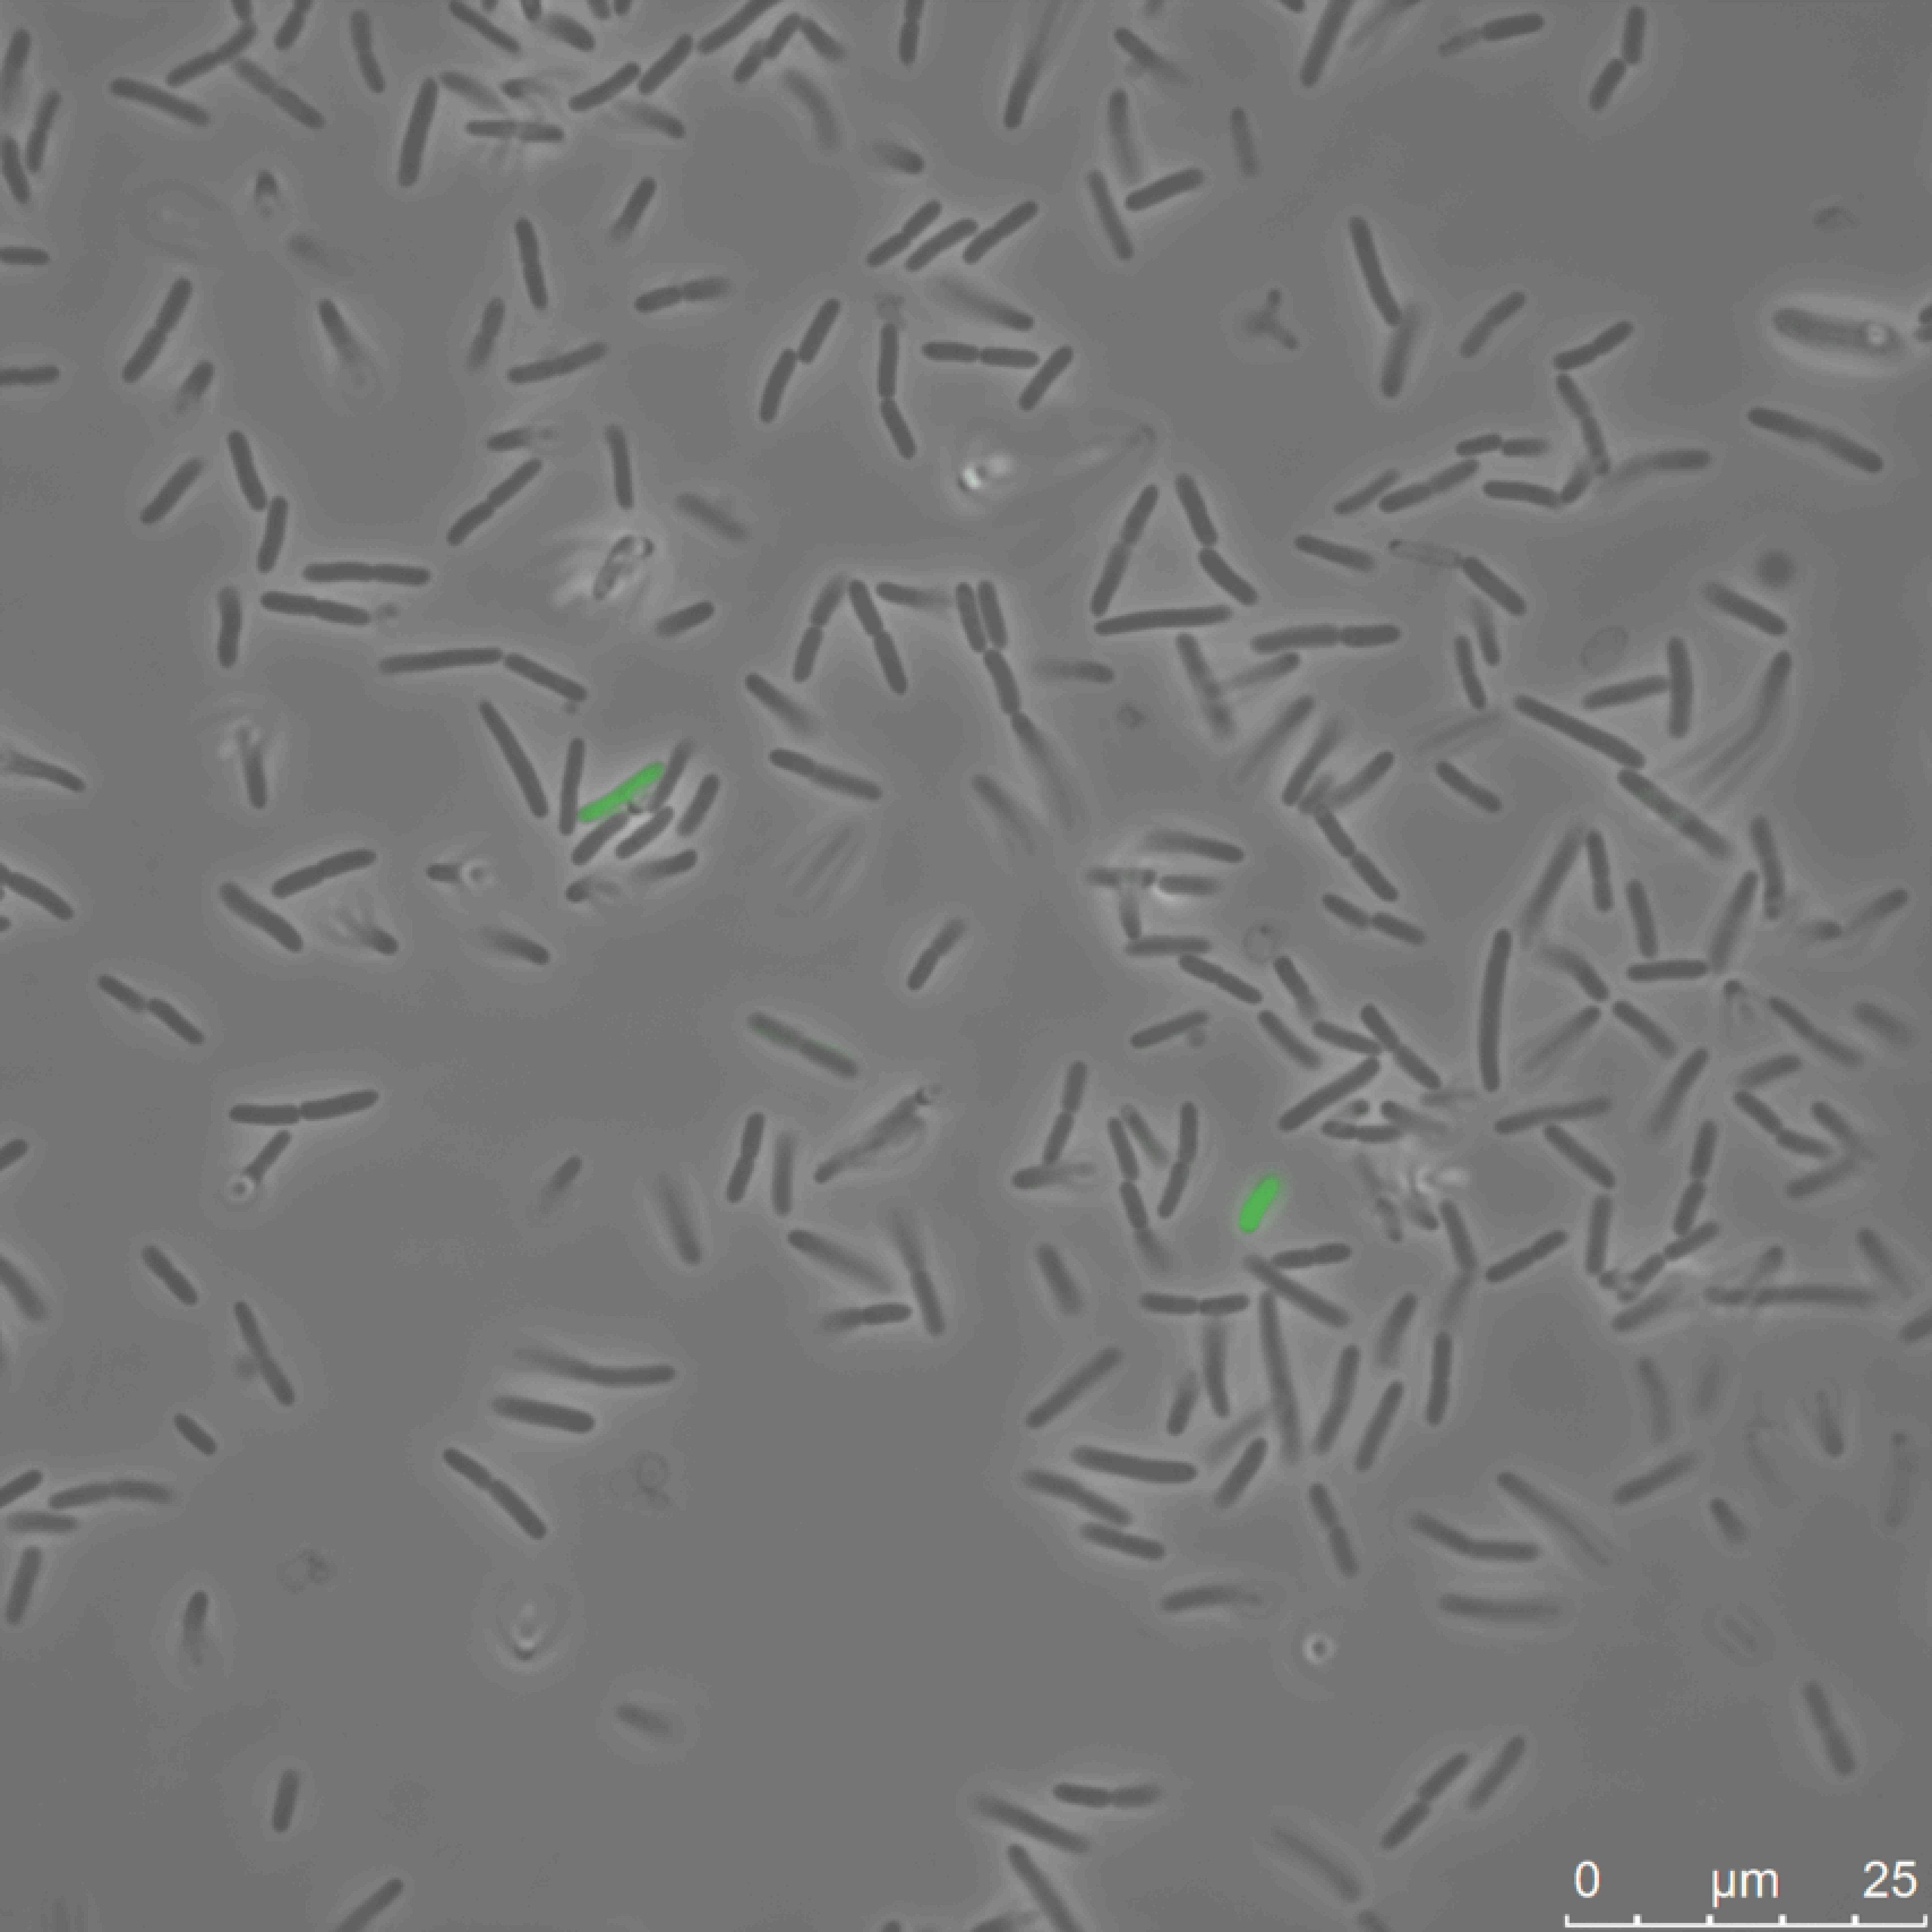
\includegraphics{TT01U4_6_GREEN-crunch-lighter-resample.pdf} &%
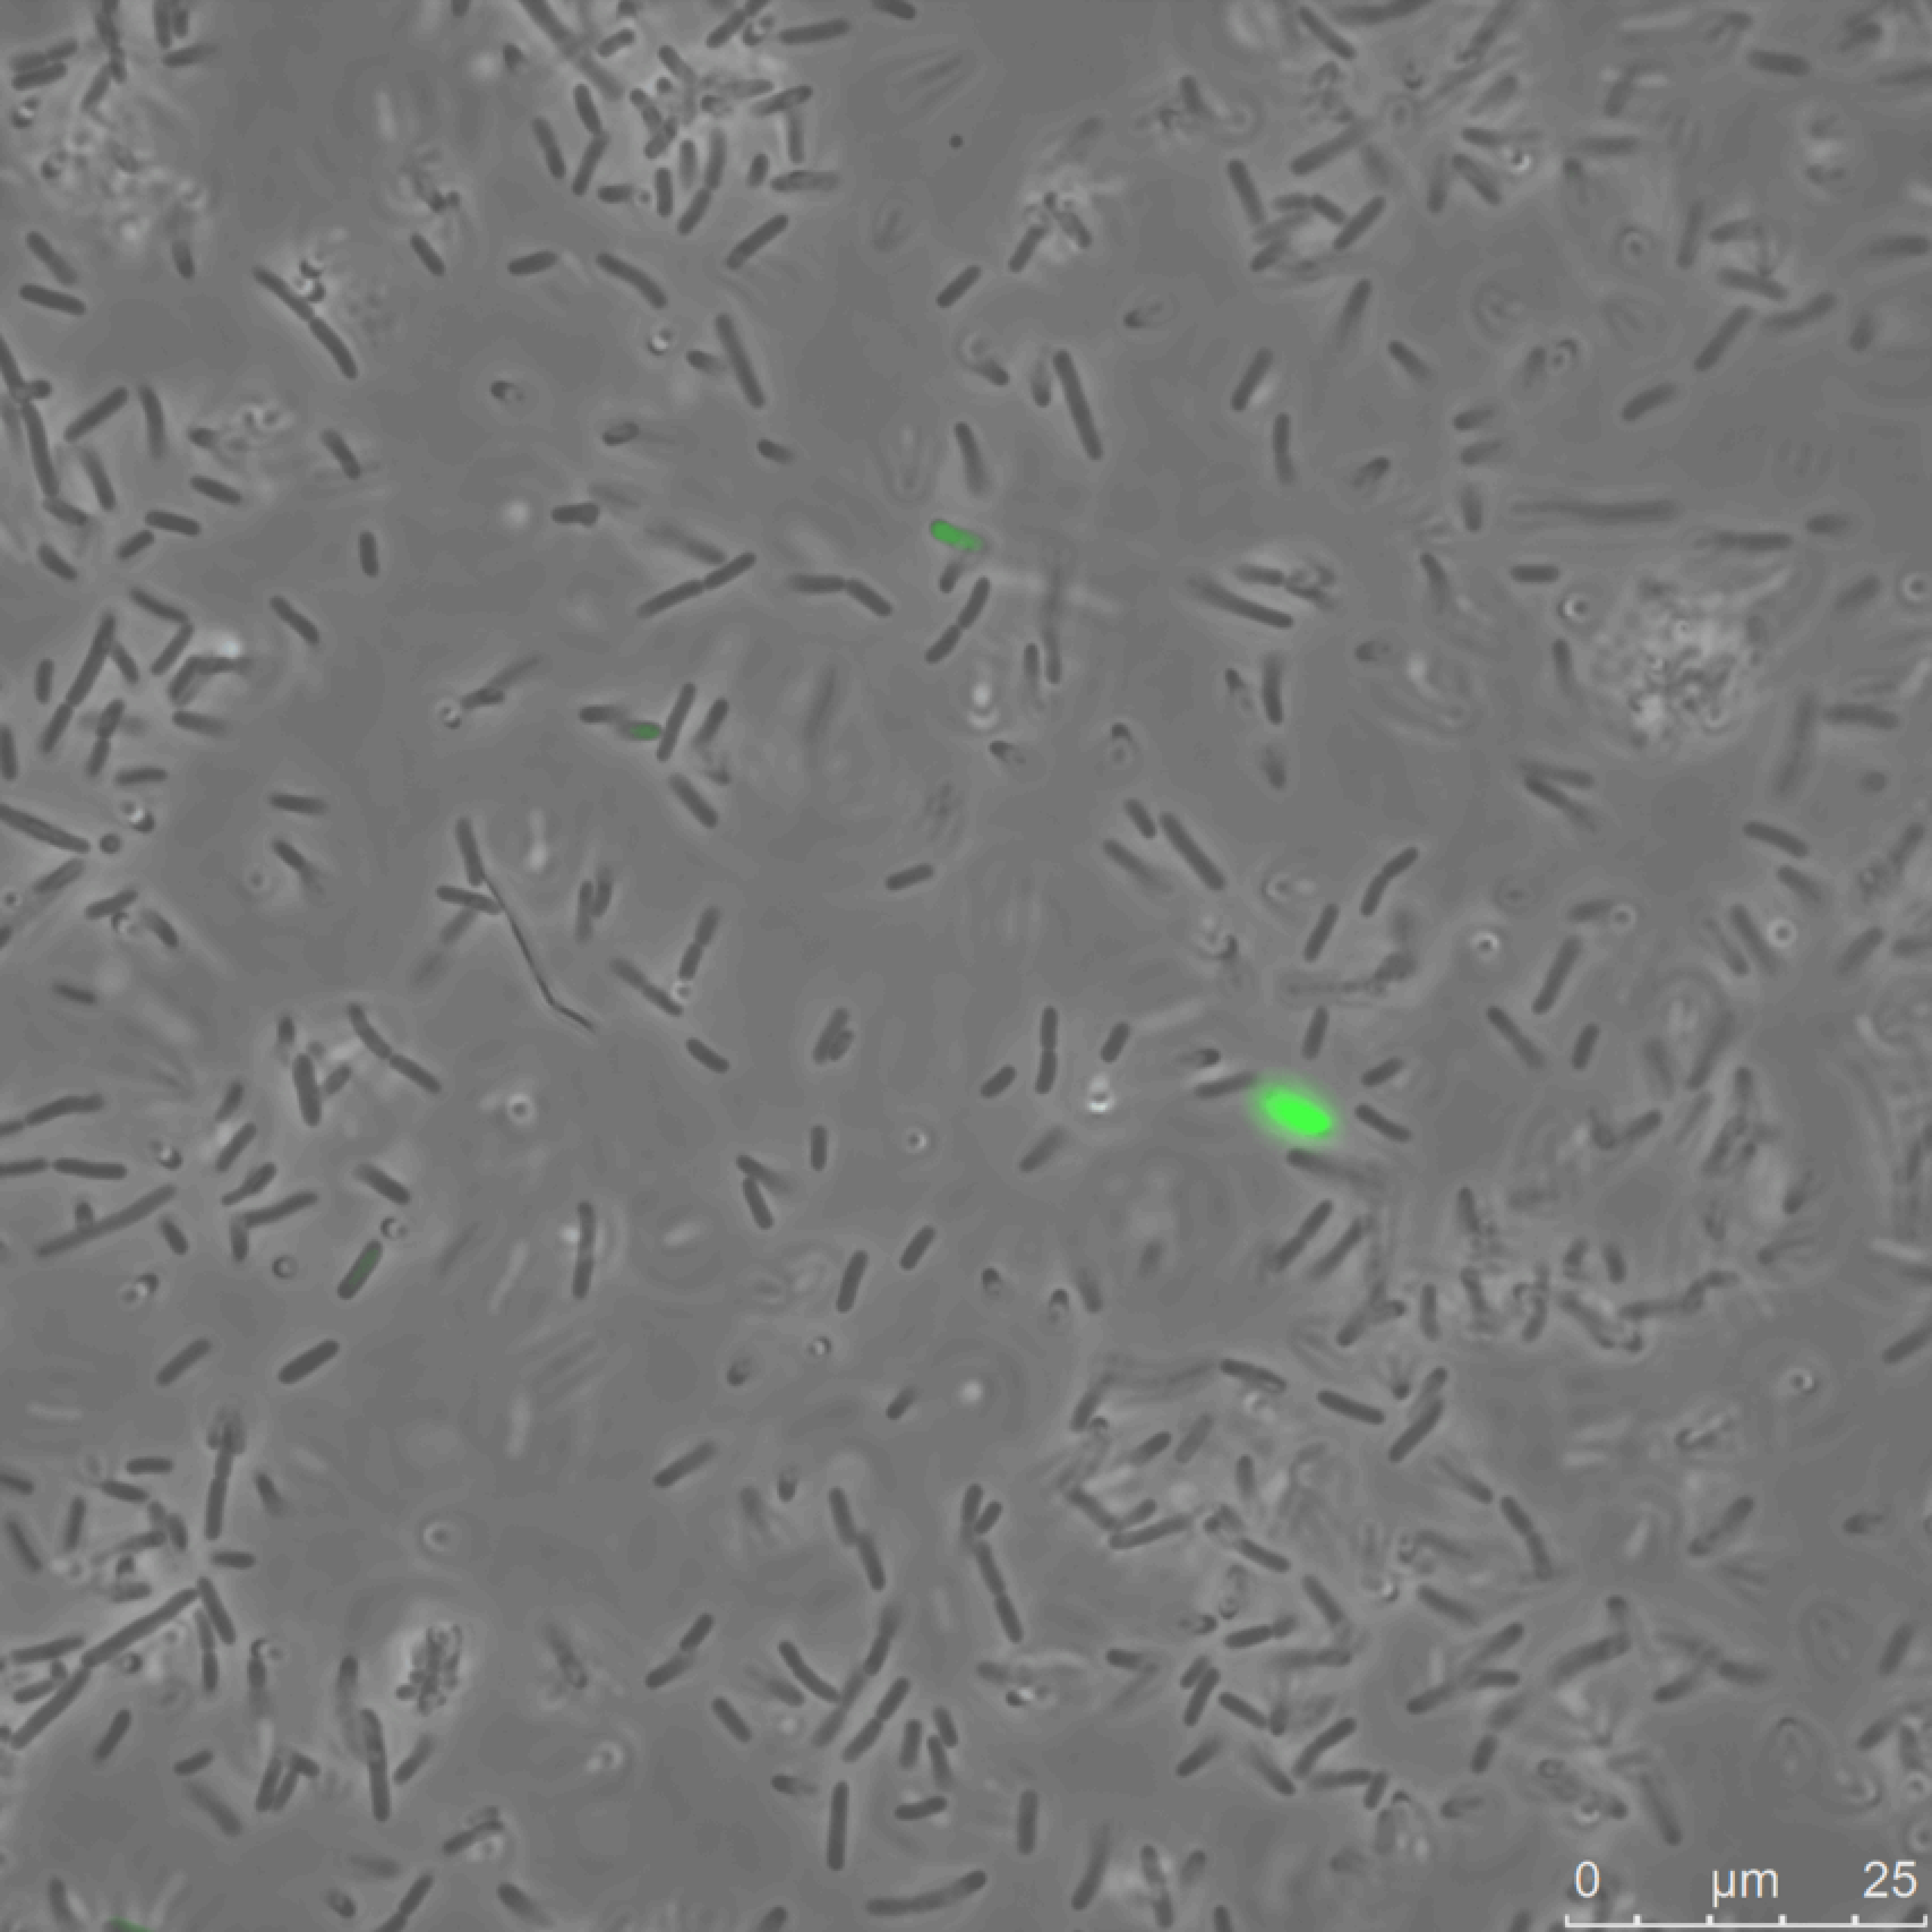
\includegraphics{TT01U4_5HR_4_GREEN-crunch-lighter-resample.pdf} &%
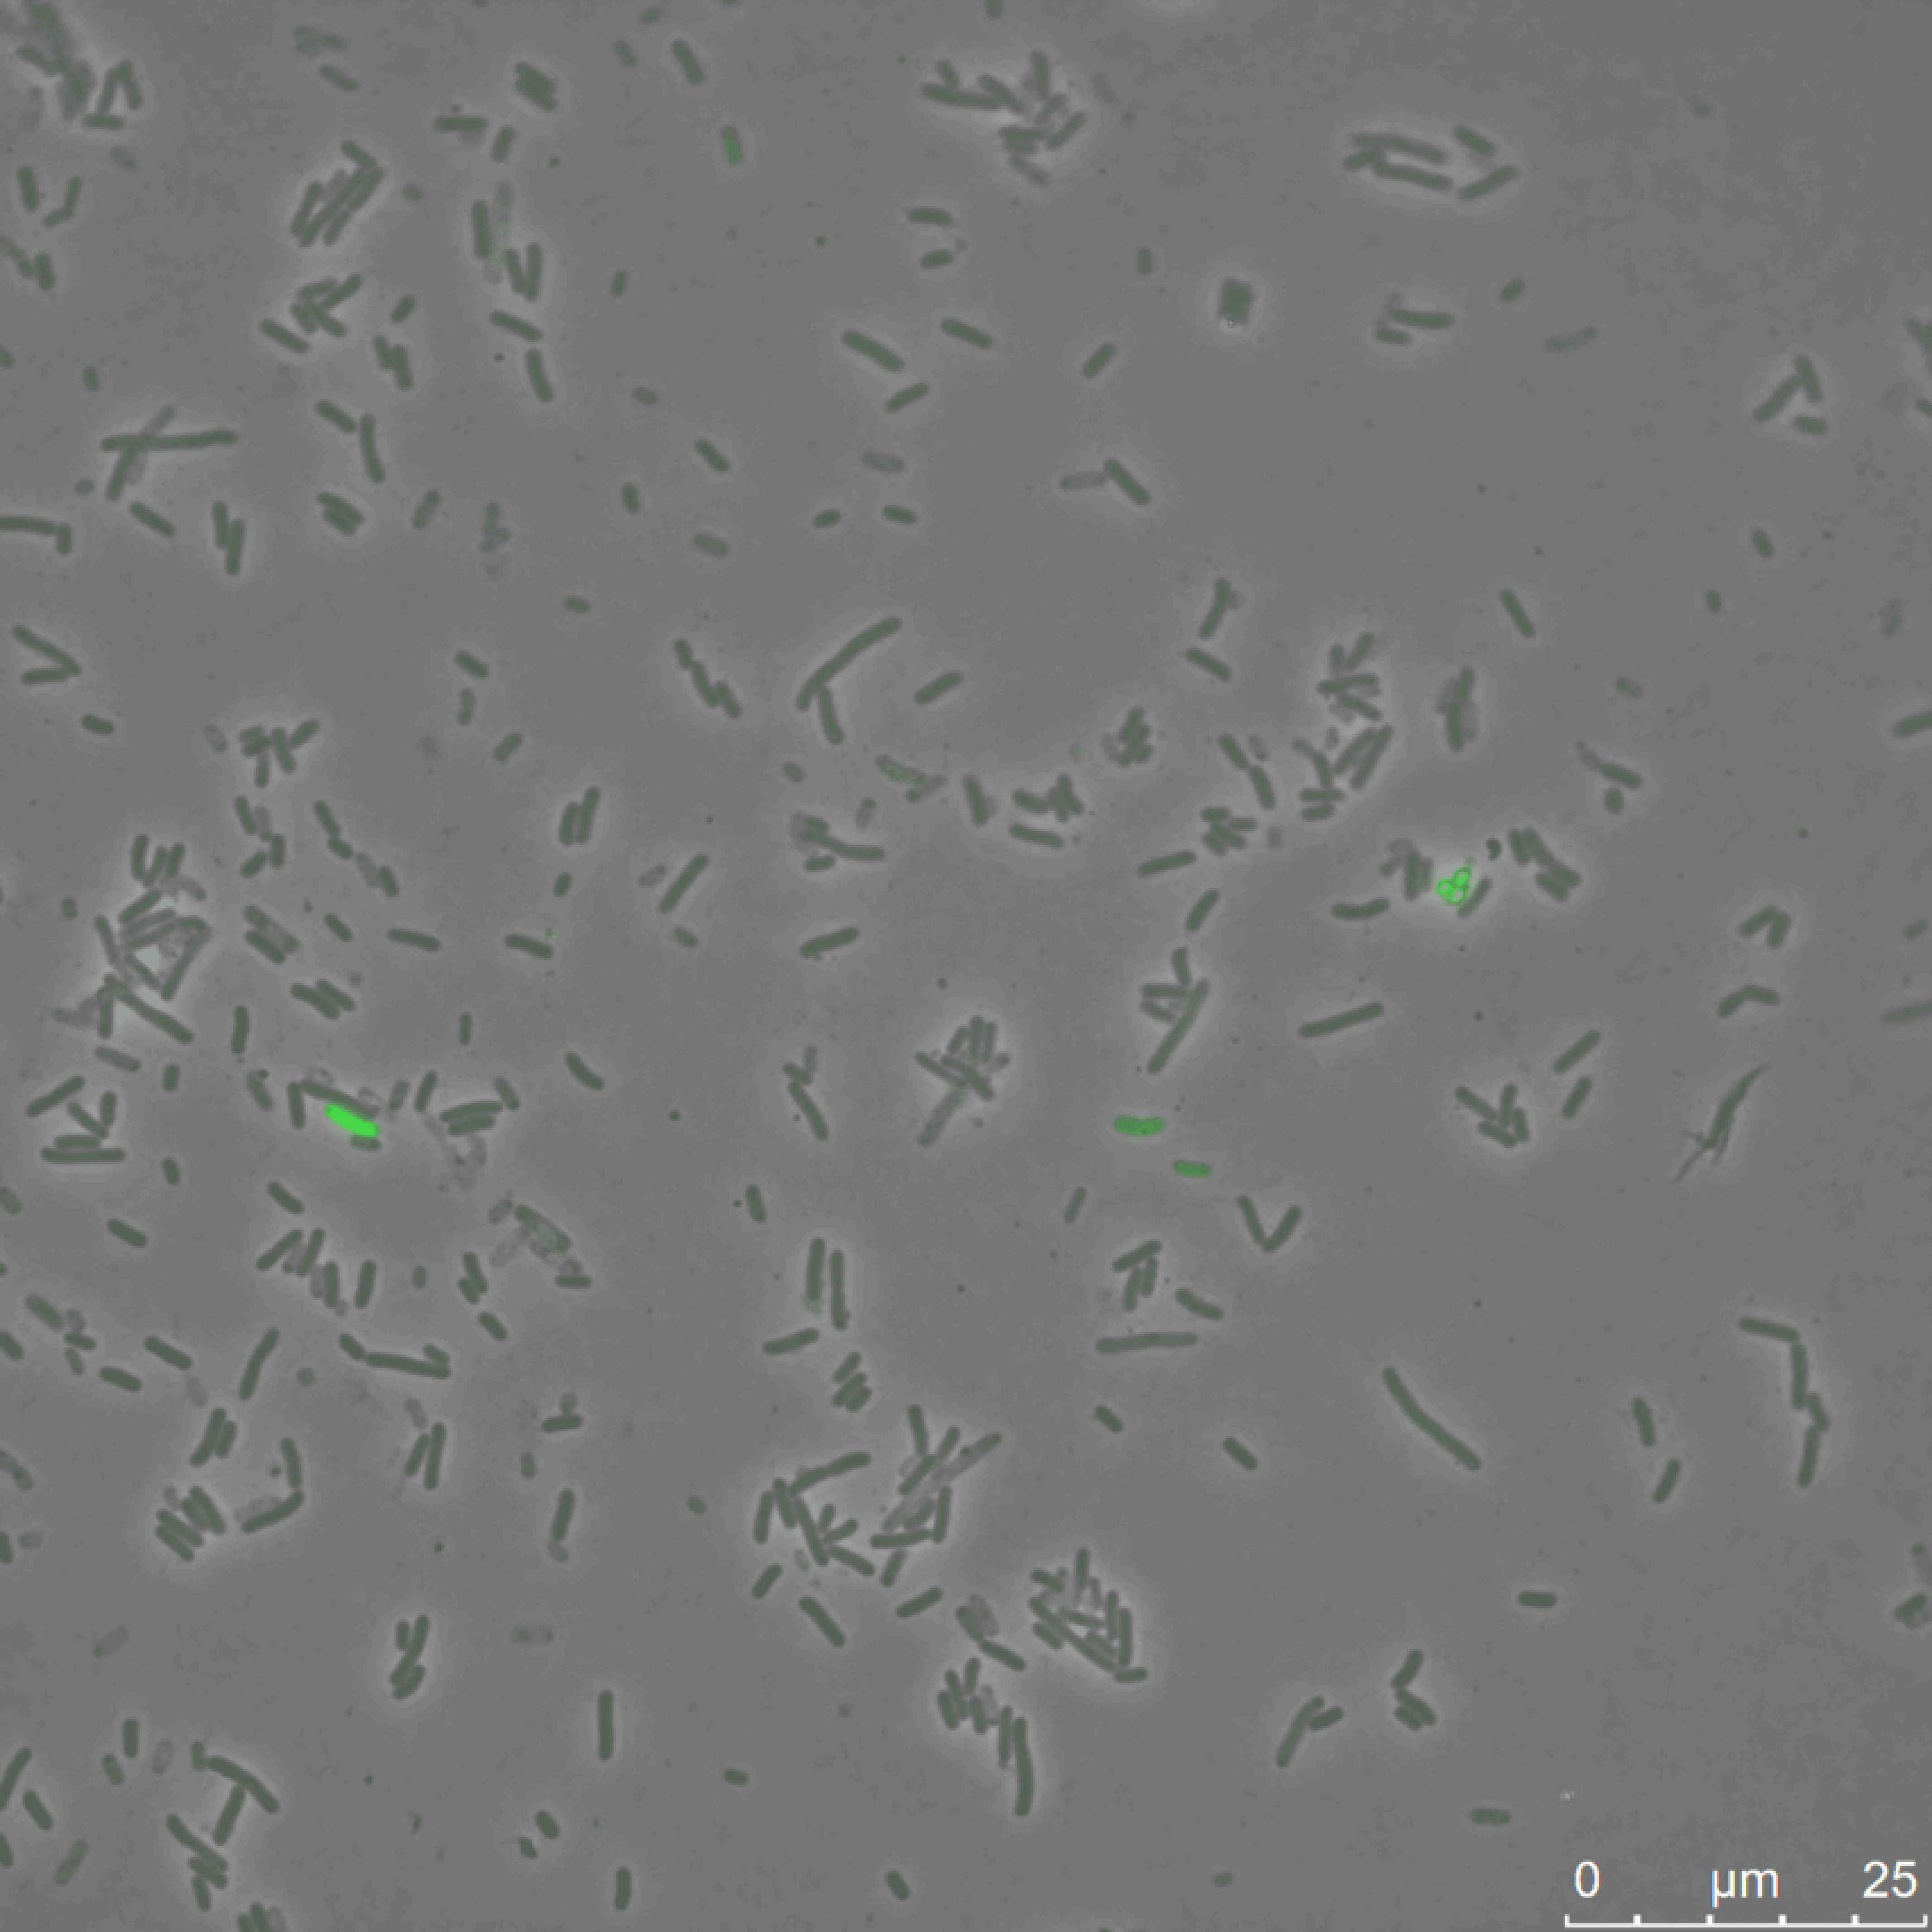
\includegraphics{TT01U4_24HR_4_GREEN-crunch-lighter-resample.pdf} &%
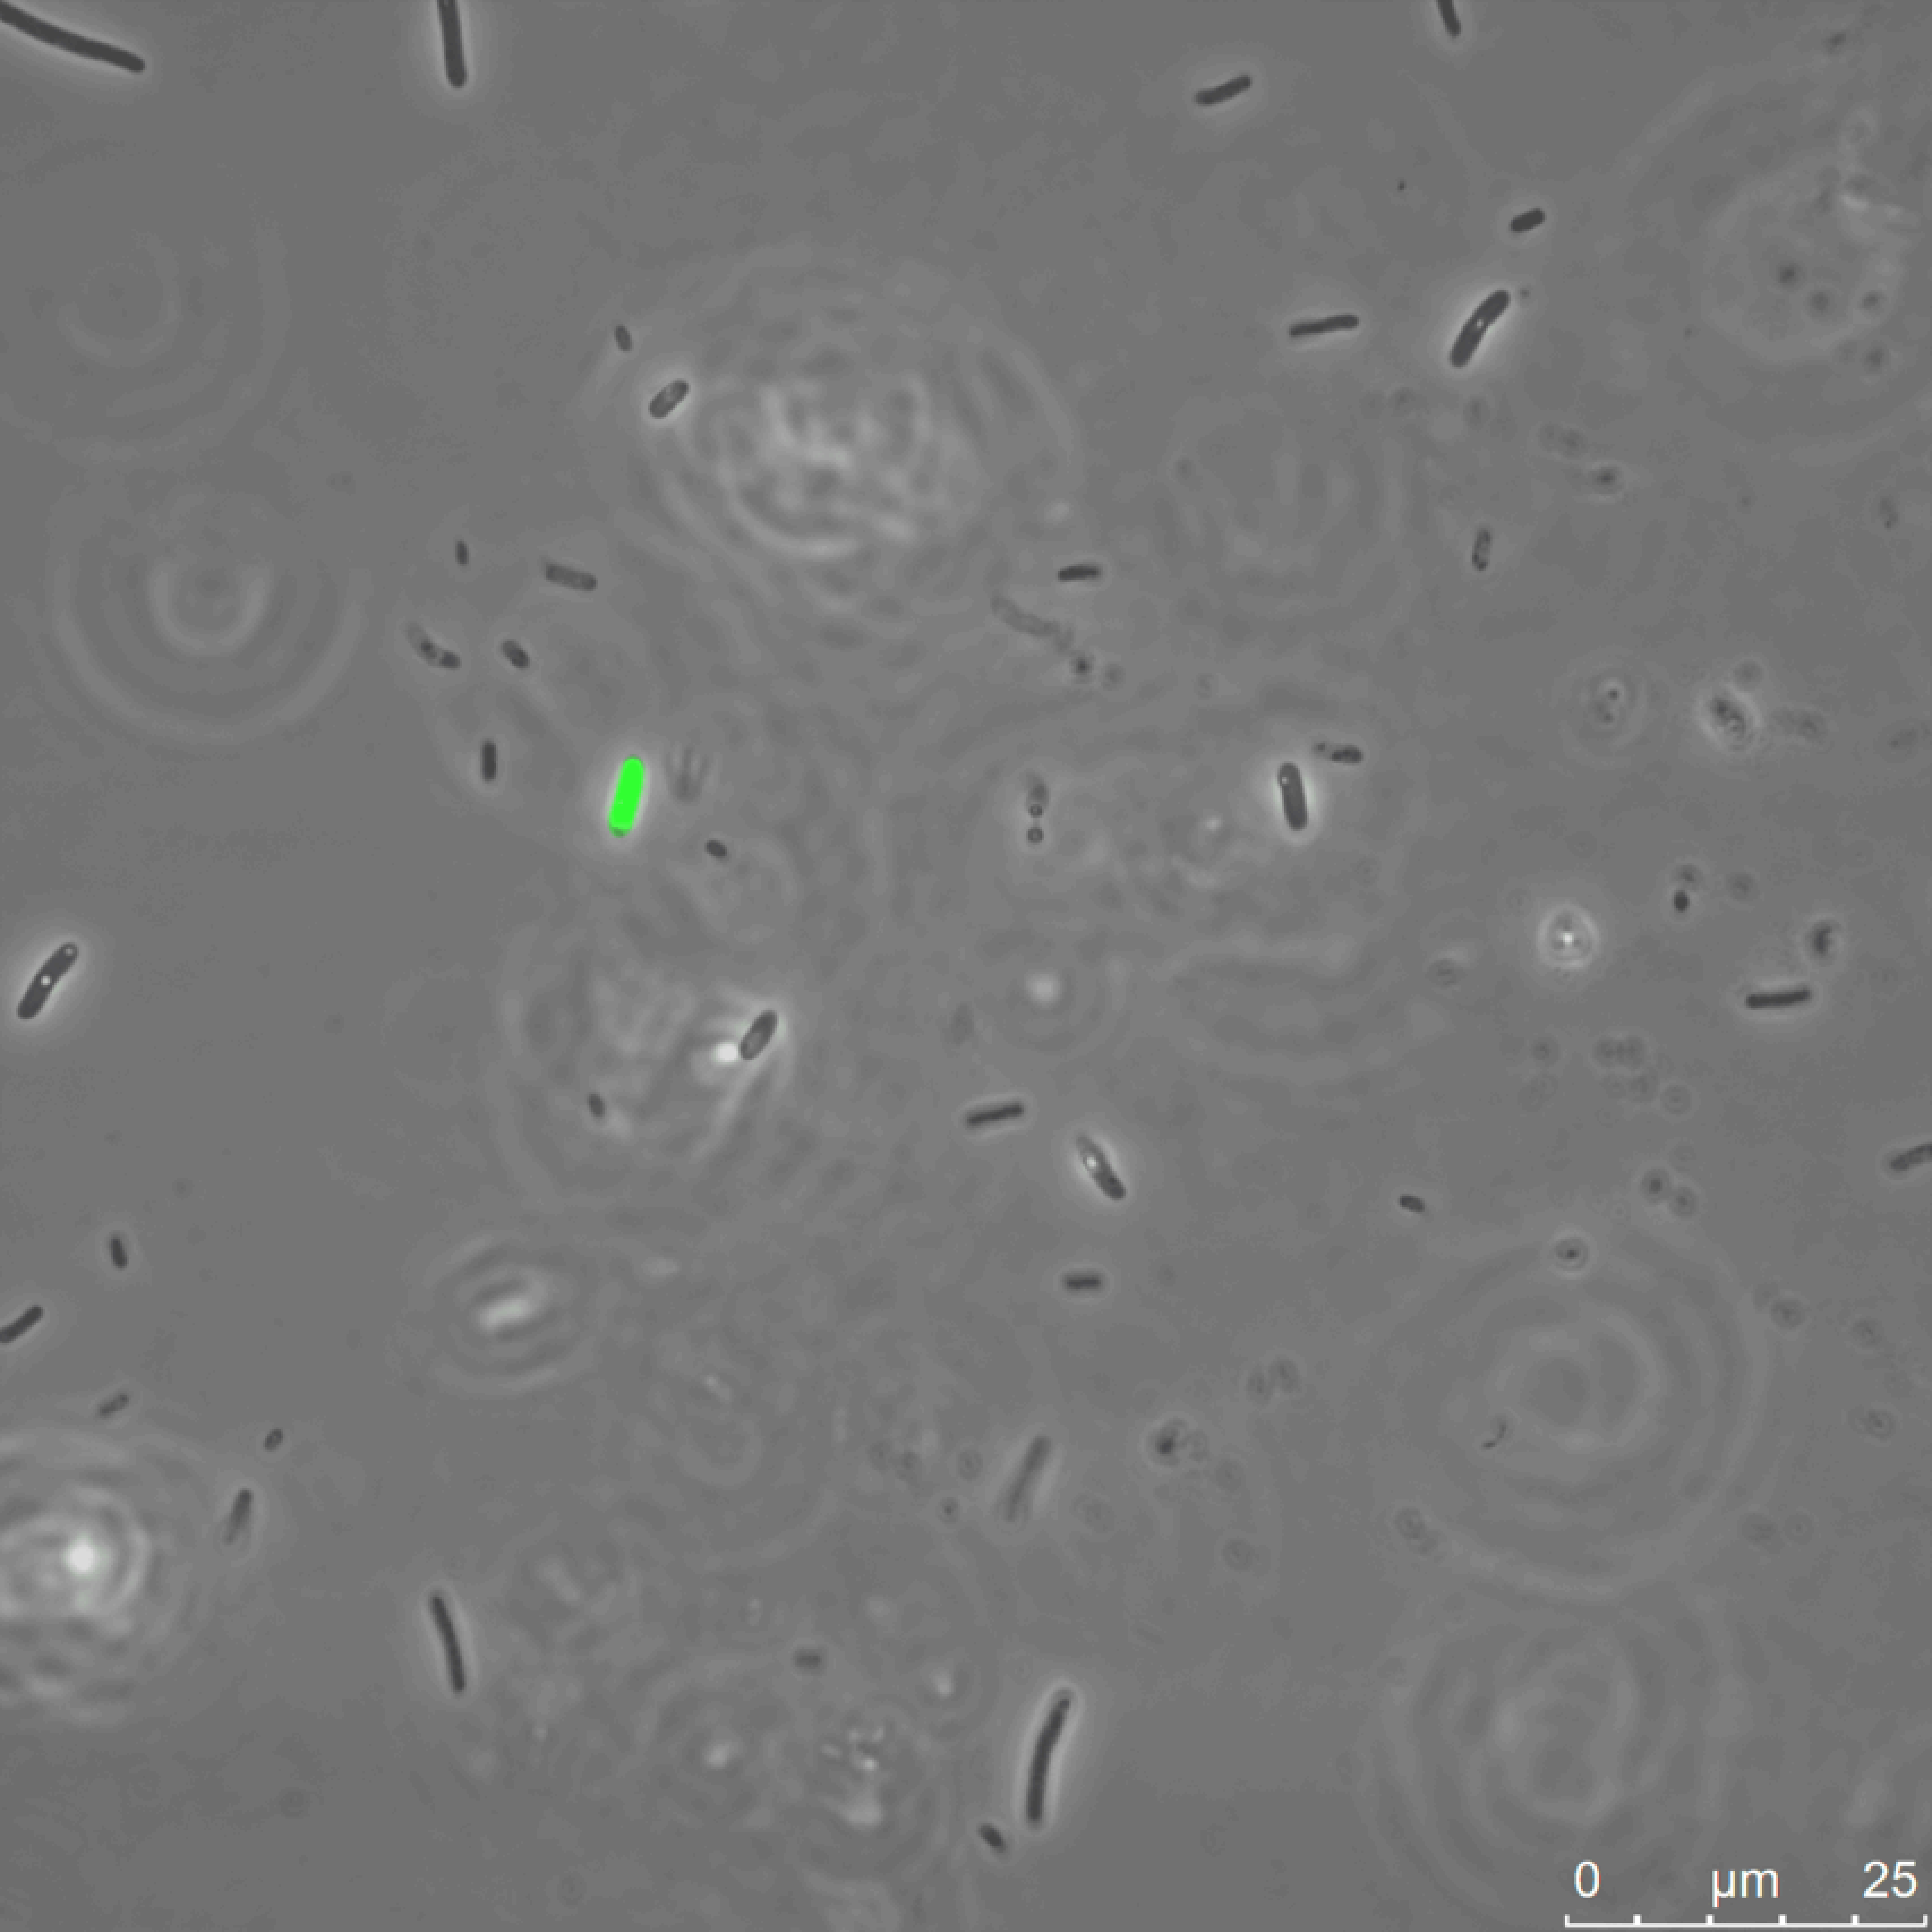
\includegraphics{TT01U4_72HR_4_GREEN-crunch-lighter-resample.pdf} \\
 ++ & ++ & ++ & ++ \\[1ex]

\end{tabularx}
\captionsetup{singlelinecheck=off, justification=justified, font=footnotesize, aboveskip=20pt}
\caption[Reporter microscopy - TT01 Unit 4]{\textsc{\normalsize Reporter microscopy for the \emph{P. luminescens} TT01 ``Unit 4" promoter.}\vspace{0.1cm} \newline A representative selection of images for 4 time points, for the PVC ``Unit 4" promoter fusion. Quadruplicate images are displayed vertically as representative of the whole slide sample. Key to qualitative fluorescence indication: ``-" - no fluorescence, ``+" - low level fluorescence in isolated cells. ``++" - low level fluorescence in many cells or few brighter cells, ``+++" - intermediate to high fluorescence in almost all cells, or very bright isolated cells.}
\end{figure}\label{RMTT01U4}
\endgroup

%%%%%%%%%%%%%%%%%%%%%%%%%%%%%%%%%%%%%%%%%%%%%%%%%%%%%%%%%%%%%%%%%%%%

\begingroup
\renewcommand{\arraystretch}{0.8}%
\setlength{\tabcolsep}{0.3pt}
\begin{figure}[p]
\setkeys{Gin}{width=\linewidth}
\Huge
\begin{tabularx}{\textwidth}{CCCC}
\multicolumn{4}{p{\linewidth}}{\large \centering \textbf{\emph{P. asymbiotica} PB68.1 (``THAI") PVC ``pnf"}} \\
\hiderowcolors
& & & \\[-1.5ex]
\Large 2 Hours &\Large 5 Hours &\Large 24 Hours &\Large 72 Hours \\[1ex]

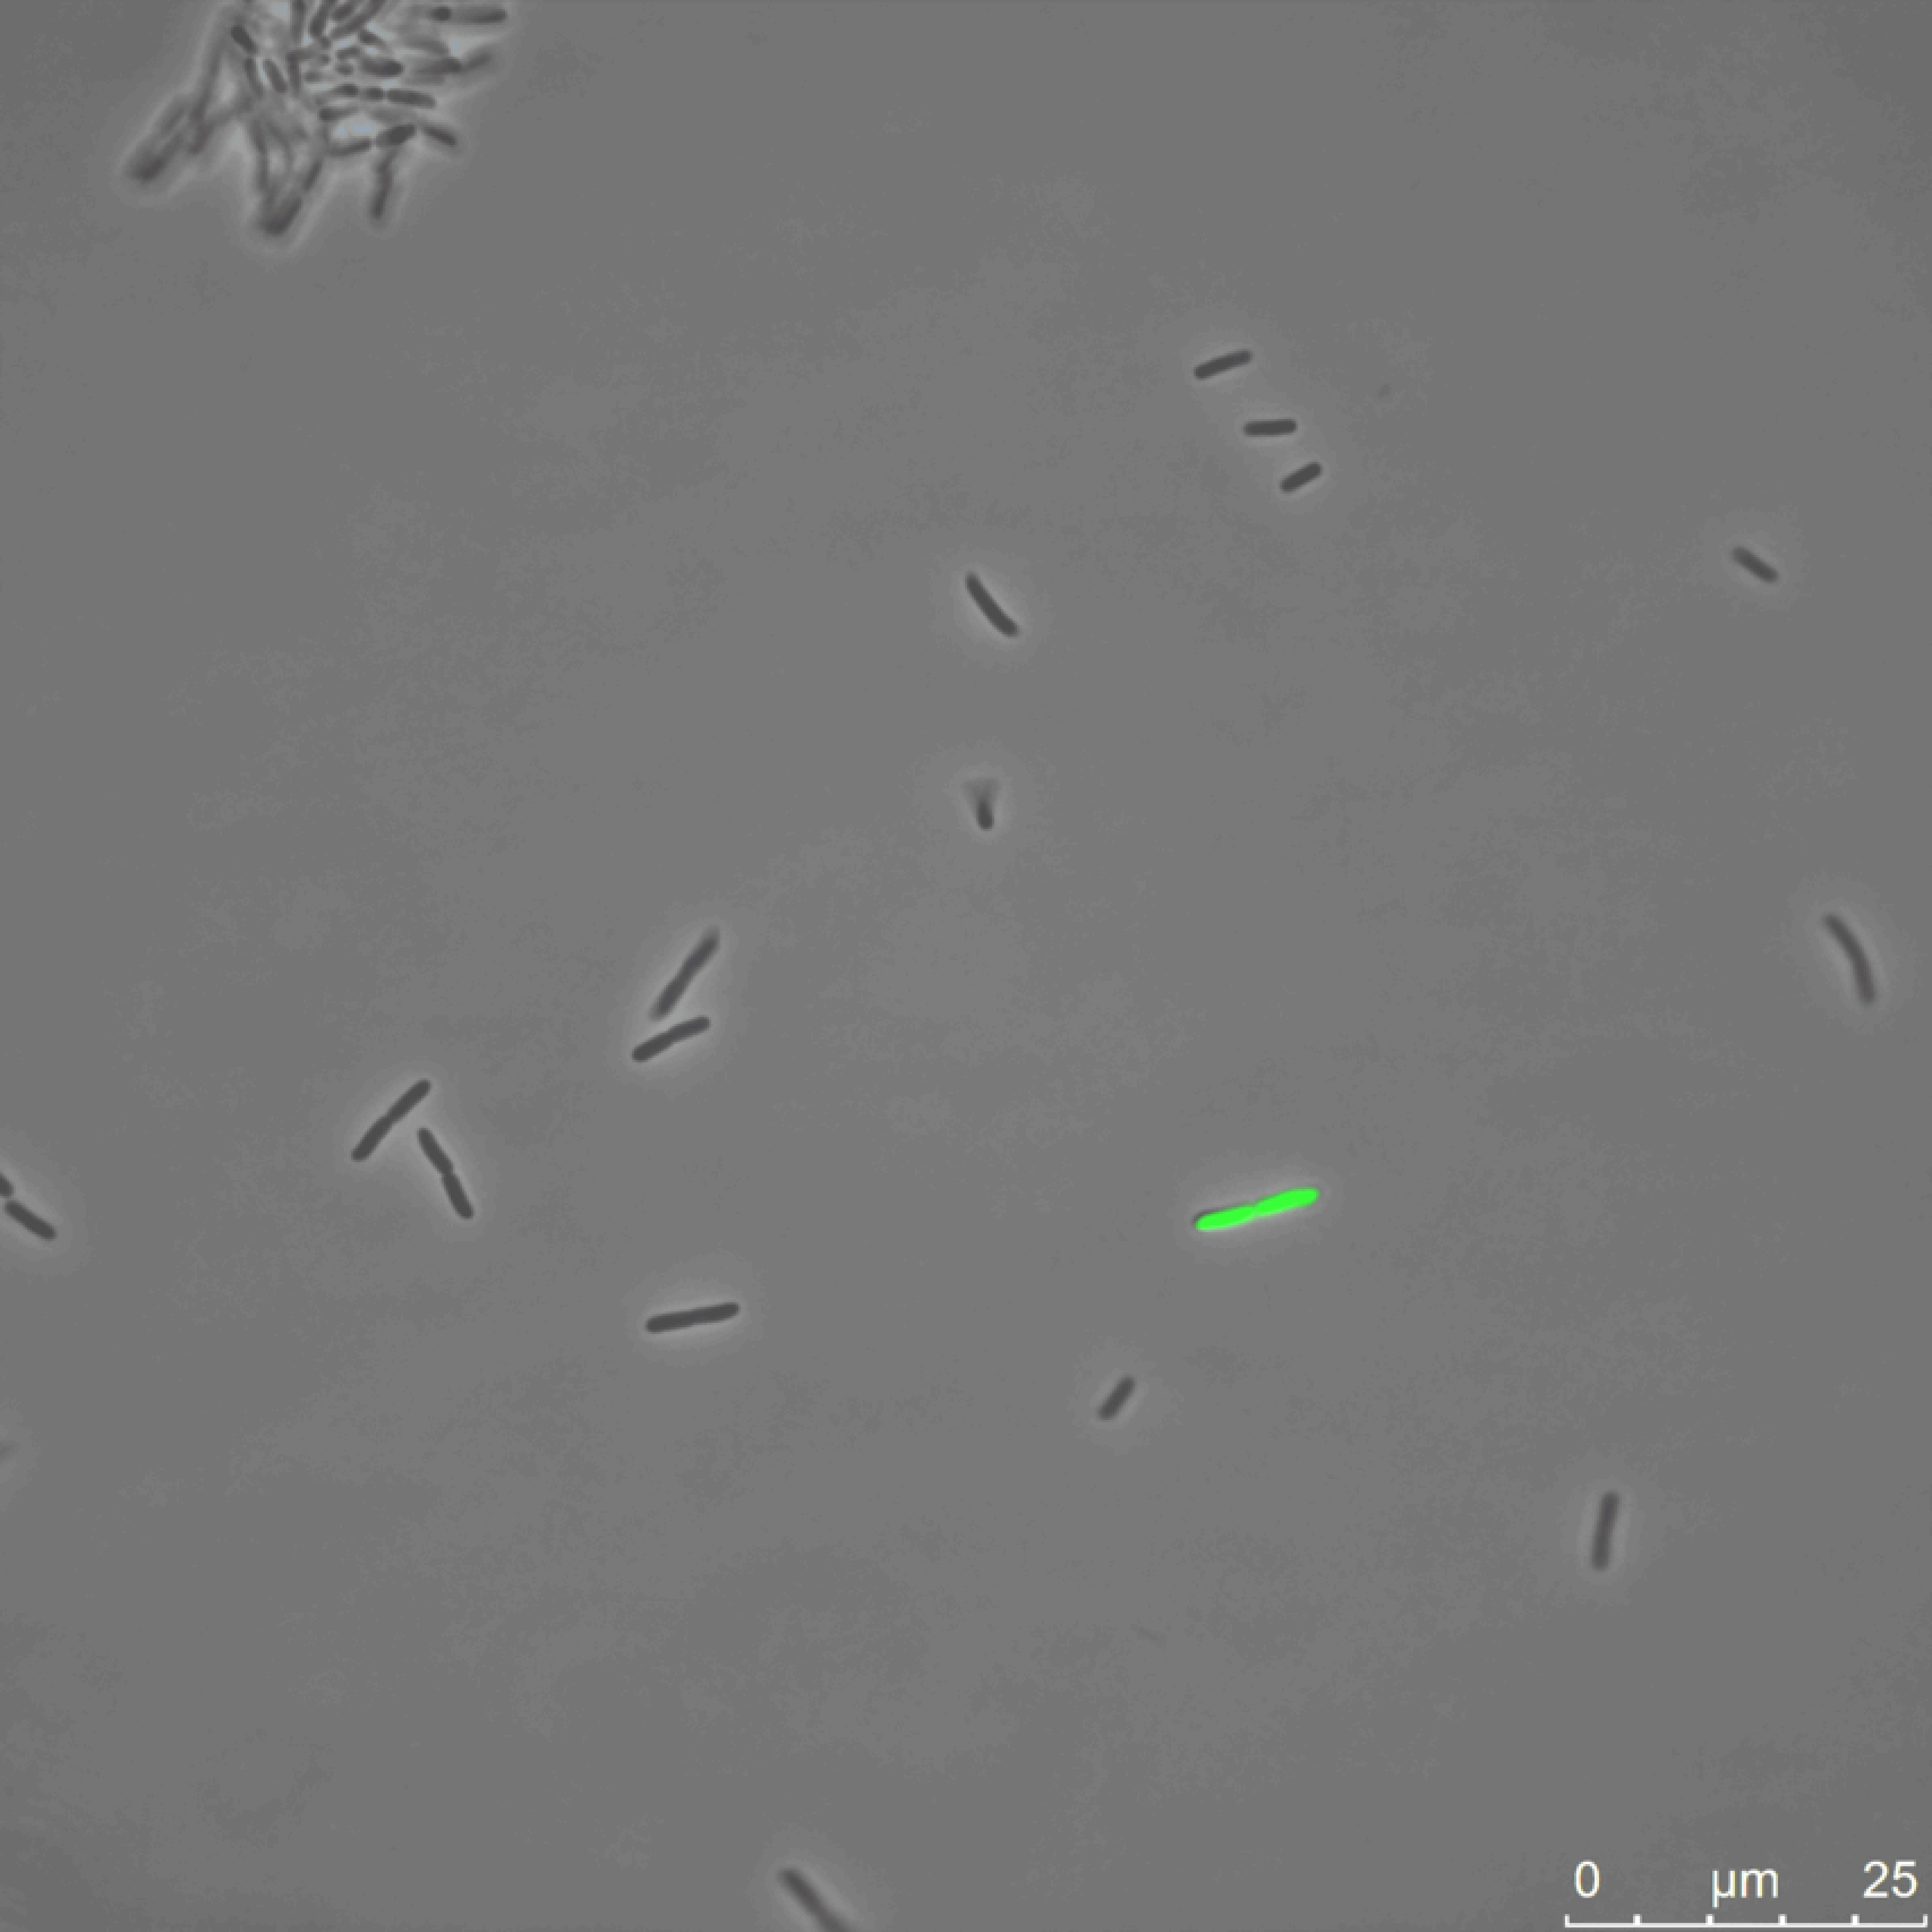
\includegraphics{THAIPNF_3_GREEN-crunch-lighter-resample.pdf} &%
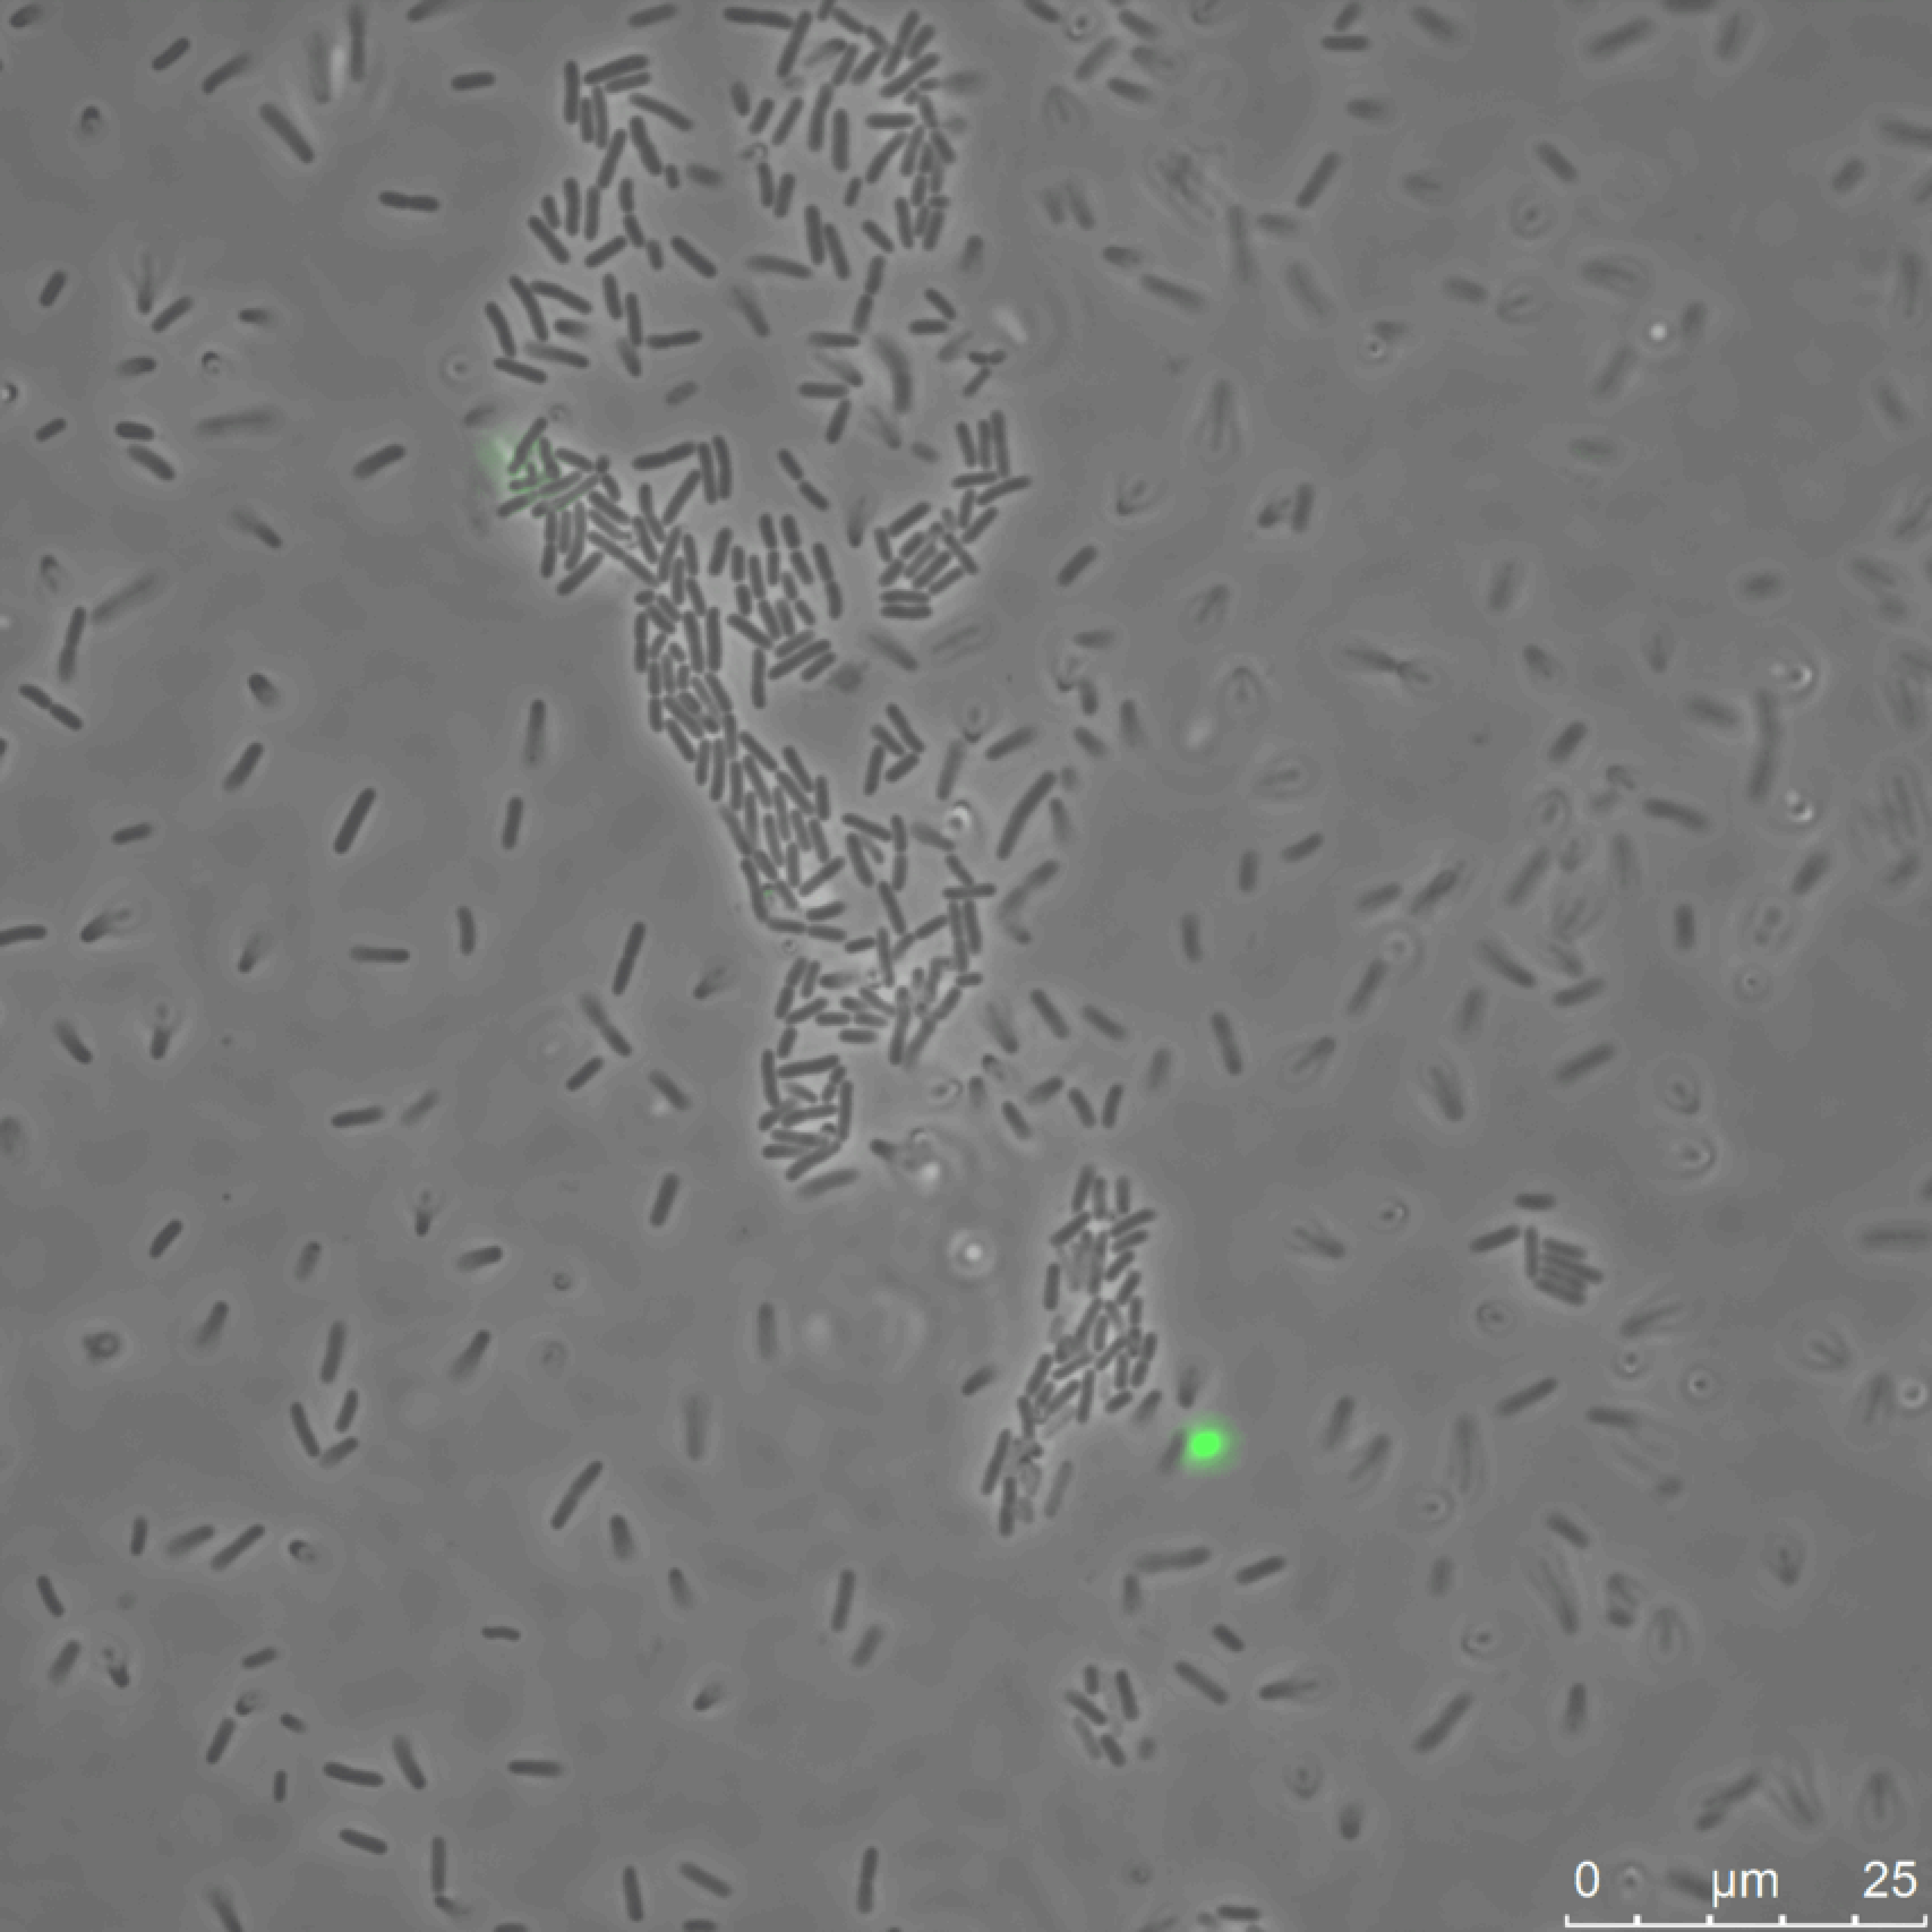
\includegraphics{THAIPNF_5HR_1_GREEN-crunch-lighter-resample.pdf} &%
\includegraphics{THAIPNF_24HR_2_GREEN-crunch-lighter-resample.pdf} &%
\includegraphics{THAIPNF_72HR_1_GREEN-crunch-lighter-resample.pdf} \\[-0.5ex]

\includegraphics{THAIPNF_4_GREEN-crunch-lighter-resample.pdf} &%
\includegraphics{THAIPNF_5HR_2_GREEN-crunch-lighter-resample.pdf} &%
\includegraphics{THAIPNF_24HR_4_GREEN-crunch-lighter-resample.pdf} &%
\includegraphics{THAIPNF_72HR_2_GREEN-crunch-lighter-resample.pdf} \\[-0.5ex]

\includegraphics{THAIPNF_5_GREEN-crunch-lighter-resample.pdf} &%
\includegraphics{THAIPNF_5HR_3_GREEN-crunch-lighter-resample.pdf} &%
\includegraphics{THAIPNF_24HR_5_GREEN-crunch-lighter-resample.pdf} &%
\includegraphics{THAIPNF_72HR_3_GREEN-crunch-lighter-resample.pdf} \\[-0.5ex]

\includegraphics{THAIPNF_6_GREEN-crunch-lighter-resample.pdf} &%
\includegraphics{THAIPNF_5HR_4_GREEN-crunch-lighter-resample.pdf} &%
\includegraphics{THAIPNF_24HR_7_GREEN-crunch-lighter-resample.pdf} &%
\includegraphics{THAIPNF_72HR_4_GREEN-crunch-lighter-resample.pdf} \\
 ++ & ++ & +++ & +++ \\[1ex]

\end{tabularx}

\captionsetup{singlelinecheck=off, justification=justified, font=footnotesize, aboveskip=20pt}
\caption[Reporter microscopy - PB68.1 pnf]{\textsc{\normalsize Reporter microscopy for the \emph{P. asymbiotica} PB68.1 ``pnf" promoter.}\vspace{0.1cm} \newline A representative selection of images for 4 time points, for the PVC ``pnf" promoter fusion. Quadruplicate images are displayed vertically as representative of the whole slide sample. Key to qualitative fluorescence indication: ``-" - no fluorescence, ``+" - low level fluorescence in isolated cells. ``++" - low level fluorescence in many cells or few brighter cells, ``+++" - intermediate to high fluorescence in almost all cells, or very bright isolated cells.}
\end{figure}\label{RMTHAIPNF}
\endgroup

%%%%%%%%%%%%%%%%%%%%%%%%%%%%%%%%%%%%%%%%%%%%%%%%%%%%%%%%%%%%%%%%%%%%

\begingroup
\renewcommand{\arraystretch}{0.8}%
\setlength{\tabcolsep}{0.3pt}
\begin{figure}[p]
\setkeys{Gin}{width=\linewidth}
\Huge
\begin{tabularx}{\textwidth}{CCCC}
\multicolumn{4}{p{\linewidth}}{\large \centering \textbf{\emph{P. luminescens} TT01 PVC ``LopT"}} \\
\hiderowcolors
& & & \\[-1.5ex]
\Large 2 Hours &\Large 5 Hours &\Large 24 Hours &\Large 72 Hours \\[1ex]

\includegraphics{TT01LOPT_1_LOWGREEN-crunch-lighter-resample.pdf} &%
\includegraphics{TT01LOPT_5HR_1_LOWGREEN-crunch-lighter-resample.pdf} &%
\includegraphics{TT01LOPT_24HR_1_GREEN-crunch-lighter-resample.pdf} &%
\includegraphics{TT01LOPT_72HR_1_GREEN-crunch-lighter-resample.pdf} \\[-0.5ex]

\includegraphics{TT01LOPT_2_NOGREEN-crunch-lighter-resample.pdf} &%
\includegraphics{TT01LOPT_5HR_2_LOWGREEN-crunch-lighter-resample.pdf} &%
\includegraphics{TT01LOPT_24HR_2_GREEN-crunch-lighter-resample.pdf} &%
\includegraphics{TT01LOPT_72HR_2_GREEN-crunch-lighter-resample.pdf} \\[-0.5ex]

\includegraphics{TT01LOPT_3_LOWGREEN-crunch-lighter-resample.pdf} &%
\includegraphics{TT01LOPT_5HR_3_LOWGREEN-crunch-lighter-resample.pdf} &%
\includegraphics{TT01LOPT_24HR_3_GREEN-crunch-lighter-resample.pdf} &%
\includegraphics{TT01LOPT_72HR_3_GREEN-crunch-lighter-resample.pdf} \\[-0.5ex]

\includegraphics{TT01LOPT_4_LOWGREEN-crunch-lighter-resample.pdf} &%
\includegraphics{TT01LOPT_5HR_4_LOWGREEN-crunch-lighter-resample.pdf} &%
\includegraphics{TT01LOPT_24HR_7_GREEN-crunch-lighter-resample.pdf} &%
\includegraphics{TT01LOPT_72HR_6_GREEN-crunch-lighter-resample.pdf} \\
 + & + & ++ & ++ \\[1ex]

\end{tabularx}

\captionsetup{singlelinecheck=off, justification=justified, font=footnotesize, aboveskip=20pt}
\caption[Reporter microscopy - TT01 LopT]{\textsc{\normalsize Reporter microscopy for the \emph{P. luminescens} TT01 ``LopT" promoter.}\vspace{0.1cm} \newline A representative selection of images for 4 time points, for the PVC ``LopT" promoter fusion. Quadruplicate images are displayed vertically as representative of the whole slide sample. Key to qualitative fluorescence indication: ``-" - no fluorescence, ``+" - low level fluorescence in isolated cells. ``++" - low level fluorescence in many cells or few brighter cells, ``+++" - intermediate to high fluorescence in almost all cells, or very bright isolated cells.}
\end{figure}\label{RMTT01LOPT}
\endgroup

%%%%%%%%%%%%%%%%%%%%%%%%%%%%%%%%%%%%%%%%%%%%%%%%%%%%%%%%%%%%%%%%%%%%


\begingroup
\renewcommand{\arraystretch}{0.8}%
\setlength{\tabcolsep}{0.3pt}
\begin{figure}[p]
\setkeys{Gin}{width=\linewidth}
\Huge
\begin{tabularx}{\textwidth}{CCCC}
\multicolumn{4}{p{\linewidth}}{\large \centering \textbf{\emph{P. asymbiotica} PB68.1 (``THAI") PVC ``LopT"}} \\
\hiderowcolors
& & & \\[-1.5ex]
\Large 2 Hours &\Large 5 Hours &\Large 24 Hours &\Large 72 Hours \\[1ex]

\includegraphics{THAILOPT_1_NOGREEN-crunch-lighter-resample.pdf} &%
\includegraphics{THAILOPT_5HR_1_NOGREEN-crunch-lighter-resample.pdf} &%
\includegraphics{THAILOPT_24HR_1_NOGREEN-crunch-lighter-resample.pdf} &%
\includegraphics{THAILOPT_72HR_1_NOGREEN-crunch-lighter-resample.pdf} \\[-0.5ex]

\includegraphics{THAILOPT_2_NOGREEN-crunch-lighter-resample.pdf} &%
\includegraphics{THAILOPT_5HR_2_NOGREEN-crunch-lighter-resample.pdf} &%
\includegraphics{THAILOPT_24HR_2_NOGREEN-crunch-lighter-resample.pdf} &%
\includegraphics{THAILOPT_72HR_2_NOGREEN-crunch-lighter-resample.pdf} \\[-0.5ex]

\includegraphics{THAILOPT_3_NOGREEN-crunch-lighter-resample.pdf} &%
\includegraphics{THAILOPT_5HR_3_NOGREEN-crunch-lighter-resample.pdf} &%
\includegraphics{THAILOPT_24HR_3_NOGREEN-crunch-lighter-resample.pdf} &%
\includegraphics{THAILOPT_72HR_3_NOGREEN-crunch-lighter-resample.pdf} \\[-0.5ex]

\includegraphics{THAILOPT_4_NOGREEN-crunch-lighter-resample.pdf} &%
\includegraphics{THAILOPT_5HR_4_NOGREEN-crunch-lighter-resample.pdf} &%
\includegraphics{THAILOPT_24HR_4_NOGREEN-crunch-lighter-resample.pdf} &%
\includegraphics{THAILOPT_72HR_4_NOGREEN-crunch-lighter-resample.pdf} \\
 - & - & - & - \\[1ex]

\end{tabularx}
\captionsetup{singlelinecheck=off, justification=justified, font=footnotesize, aboveskip=20pt}
\caption[Reporter microscopy - PB68.1 LopT]{\textsc{\normalsize Reporter microscopy for the \emph{P. asymbiotica} PB68.1 ``LopT" promoter.}\vspace{0.1cm} \newline A representative selection of images for 4 time points, for the PVC ``LopT" promoter fusion. Quadruplicate images are displayed vertically as representative of the whole slide sample. Key to qualitative fluorescence indication: ``-" - no fluorescence, ``+" - low level fluorescence in isolated cells. ``++" - low level fluorescence in many cells or few brighter cells, ``+++" - intermediate to high fluorescence in almost all cells, or very bright isolated cells.}
\end{figure}\label{RMTHAILOPT}
\endgroup

%%%%%%%%%%%%%%%%%%%%%%%%%%%%%%%%%%%%%%%%%%%%%%%%%%%%%%%%%%%%%%%%%%%%


\begingroup
\renewcommand{\arraystretch}{0.8}%
\setlength{\tabcolsep}{0.3pt}
\begin{figure}[p]
\setkeys{Gin}{width=\linewidth}
\Huge
\begin{tabularx}{\textwidth}{CCCC}
\multicolumn{4}{p{\linewidth}}{\large \centering \textbf{\emph{P. luminescens} TT01 PVC ``Cif"}} \\
\hiderowcolors
& & & \\[-1.5ex]
\Large 2 Hours &\Large 5 Hours &\Large 24 Hours &\Large 72 Hours \\[1ex]

\includegraphics{TT01CIF_1_NOGREEN-crunch-lighter-resample.pdf} &%
\includegraphics{TT01CIF_5HR_1_LOWGREEN-crunch-lighter-resample.pdf} &%
\includegraphics{TT01CIF_24HR_6_GREEN-crunch-lighter-resample.pdf} &%
\includegraphics{TT01CIF_72HR_5_GREEN-crunch-lighter-resample.pdf} \\[-0.5ex]

\includegraphics{TT01CIF_2_NOGREEN-crunch-lighter-resample.pdf} &%
\includegraphics{TT01CIF_5HR_2_LOWGREEN-crunch-lighter-resample.pdf} &%
\includegraphics{TT01CIF_24HR_2_GREEN-crunch-lighter-resample.pdf} &%
\includegraphics{TT01CIF_72HR_7_GREEN-crunch-lighter-resample.pdf} \\[-0.5ex]

\includegraphics{TT01CIF_3_NOGREEN-crunch-lighter-resample.pdf} &%
\includegraphics{TT01CIF_5HR_3_LOWGREEN-crunch-lighter-resample.pdf} &%
\includegraphics{TT01CIF_24HR_3_GREEN-crunch-lighter-resample.pdf} &%
\includegraphics{TT01CIF_72HR_3_GREEN-crunch-lighter-resample.pdf} \\[-0.5ex]

\includegraphics{TT01CIF_4_LOWGREEN-crunch-lighter-resample.pdf} &%
\includegraphics{TT01CIF_5HR_5_LOWGREEN-crunch-lighter-resample.pdf} &%
\includegraphics{TT01CIF_24HR_4_GREEN-crunch-lighter-resample.pdf} &%
\includegraphics{TT01CIF_72HR_6_GREEN-crunch-lighter-resample.pdf} \\
 - & + & ++ & ++ \\[1ex]

\end{tabularx}
\captionsetup{singlelinecheck=off, justification=justified, font=footnotesize, aboveskip=20pt}
\caption[Reporter microscopy - TT01 Cif]{\textsc{\normalsize Reporter microscopy for the \emph{P. luminescens} TT01 ``Cif" promoter.}\vspace{0.1cm} \newline A representative selection of images for 4 time points, for the PVC ``Cif" promoter fusion. Quadruplicate images are displayed vertically as representative of the whole slide sample. Key to qualitative fluorescence indication: ``-" - no fluorescence, ``+" - low level fluorescence in isolated cells. ``++" - low level fluorescence in many cells or few brighter cells, ``+++" - intermediate to high fluorescence in almost all cells, or very bright isolated cells.}
\end{figure}\label{RMTT01CIF}
\endgroup

%%%%%%%%%%%%%%%%%%%%%%%%%%%%%%%%%%%%%%%%%%%%%%%%%%%%%%%%%%%%%%%%%%%%


\begingroup
\renewcommand{\arraystretch}{0.8}%
\setlength{\tabcolsep}{0.3pt}
\begin{figure}[p]
\setkeys{Gin}{width=\linewidth}
\Huge
\begin{tabularx}{\textwidth}{CCCC}
\multicolumn{4}{p{\linewidth}}{\large \centering \textbf{\emph{P. asymbiotica} PB68.1 (``THAI") PVC ``Cif"}} \\
\hiderowcolors
& & & \\[-1.5ex]
\Large 2 Hours &\Large 5 Hours &\Large 24 Hours &\Large 72 Hours \\[1ex]

\includegraphics{THAICIF_1_LOWGREEN-crunch-lighter-resample.pdf} &%
\includegraphics{THAICIF_5HR_1_NOGREEN-crunch-lighter-resample.pdf} &%
\includegraphics{THAICIF_24HR_5_GREEN-crunch-lighter-resample.pdf} &%
\includegraphics{THAICIF_72HR_1_GREEN-crunch-lighter-resample.pdf} \\[-0.5ex]

\includegraphics{THAICIF_2_LOWGREEN-crunch-lighter-resample.pdf} &%
\includegraphics{THAICIF_5HR_2_LOWGREEN-crunch-lighter-resample.pdf} &%
\includegraphics{THAICIF_24HR_6_GREEN-crunch-lighter-resample.pdf} &%
\includegraphics{THAICIF_72HR_2_GREEN-crunch-lighter-resample.pdf} \\[-0.5ex]

\includegraphics{THAICIF_3_LOWGREEN-crunch-lighter-resample.pdf} &%
\includegraphics{THAICIF_5HR_3_NOGREEN-crunch-lighter-resample.pdf} &%
\includegraphics{THAICIF_24HR_3_GREEN-crunch-lighter-resample.pdf} &%
\includegraphics{THAICIF_72HR_3_GREEN-crunch-lighter-resample.pdf} \\[-0.5ex]

\includegraphics{THAICIF_4_LOWGREEN-crunch-lighter-resample.pdf} &%
\includegraphics{THAICIF_5HR_4_NOGREEN-crunch-lighter-resample.pdf} &%
\includegraphics{THAICIF_24HR_4_GREEN-crunch-lighter-resample.pdf} &%
\includegraphics{THAICIF_72HR_5_GREEN-crunch-lighter-resample.pdf} \\
 + & + & +++ & ++ \\[1ex]

\end{tabularx}
\captionsetup{singlelinecheck=off, justification=justified, font=footnotesize, aboveskip=20pt}
\caption[Reporter microscopy - PB68.1 Cif]{\textsc{\normalsize Reporter microscopy for the \emph{P. asymbiotica} PB68.1 ``Cif" promoter.}\vspace{0.1cm} \newline A representative selection of images for 4 time points, for the PVC ``Cif" promoter fusion. Quadruplicate images are displayed vertically as representative of the whole slide sample. Key to qualitative fluorescence indication: ``-" - no fluorescence, ``+" - low level fluorescence in isolated cells. ``++" - low level fluorescence in many cells or few brighter cells, ``+++" - intermediate to high fluorescence in almost all cells, or very bright isolated cells.}
\end{figure}\label{RMTHAICIF}

\endgroup

%%%%%%%%%%%%%%%%%%%%%%%%%%%%%%%%%%%%%%%%%%%%%%%%%%%%%%%%%%%%%%%%%%%%

\begingroup
\renewcommand{\arraystretch}{0.8}%
\setlength{\tabcolsep}{0.3pt}
\begin{figure}[p]
\setkeys{Gin}{width=\linewidth}
\Huge
\begin{tabularx}{\textwidth}{CCCC}
\multicolumn{4}{p{\linewidth}}{\large \centering \textbf{\emph{P. luminescens} TT01 pAGAG Negative Control}} \\
\hiderowcolors
& & & \\[-1.5ex]
\Large 2 Hours &\Large 5 Hours &\Large 24 Hours &\Large 72 Hours \\[1ex]

\includegraphics{TT01_pAGAG_CONTROL-crunch-lighter-resample.pdf} &%
\includegraphics{TT01_pAGAG_5HR_CONTROL-crunch-lighter-resample.pdf} &%
\includegraphics{TT01_pAGAG_24HR_CONTROL-crunch-lighter-resample.pdf} &%
\includegraphics{TT01_pAGAG_72HR_CONTROL-crunch-lighter-resample.pdf} \\[-0.5ex]


\multicolumn{4}{p{\linewidth}}{\large \centering \textbf{\emph{P. asymbiotica} PB68.1 (``THAI") pAGAG Negative Control}} \\

\includegraphics{THAI_pAGAG_CONTROL-crunch-lighter-resample.pdf} &%
\includegraphics{THAI_pAGAG_5HR_CONTROL-crunch-lighter-resample.pdf} &%
\includegraphics{THAI_pAGAG_24HR_CONTROL-crunch-lighter-resample.pdf} &%
\includegraphics{THAI_pAGAG_72HR_CONTROL-crunch-lighter-resample.pdf} \\[-0.5ex]

 - & - & - & - \\[1ex]

\end{tabularx}

\captionsetup{singlelinecheck=off, justification=justified, font=footnotesize, aboveskip=20pt}
\caption[Reporter microscopy - pAGAG Controls]{\textsc{\normalsize Reporter microscopy for empty vector control plasmids.}\vspace{0.1cm} \newline A representative selection of images for 4 time points, for \emph{P. luminenscens} TT01 and \emph{P. asymbiotica} PB68.1 bearing `empty' vectors, lacking promotors to ensure no background fluorescence or leaky expression. Key to qualitative fluorescence indication: ``-" - no fluorescence, ``+" - low level fluorescence in isolated cells. ``++" - low level fluorescence in many cells or few brighter cells, ``+++" - intermediate to high fluorescence in almost all cells, or very bright isolated cells.}
\end{figure}\label{RMpAGAG}
\endgroup




















\subsection{A putative role for RfaH in PVC regulation}

Alignment of RfaH - AnfA1 and any other ops active proteins?

RfaH sequence = \emph{ops} GGCGGTAGnnTG (in e coli) \citep{Sevostyanova2008, Artsimovitch2002}

Show/state that the JUMPStart sequence is closely related (contains an ops), but there doesn't appear to be a compelling structure for it in PVCs

Mention BW2115 knock out having weird morphology, and RfaH couldnt be knocked out in Photo
 - Mention that RfaH was initially thought to be essential in the first wave of keio knockouts but later was able to be removed.

Add the AFP 5' UTR to the alignment?

\begin{figure}[p]
\vspace{-0.5cm}
\begin{texshade}{/Users/joehealey/Documents/Warwick/PhD/Thesis/chapters/chapter6/resources/alignments/PVC_upstream_w_RfaH.afasta}
\seqtype{N}
\setends{19}{0..180}
\setfont{numbering}{tt}{md}{sc}{tiny}
\setfont{names}{tt}{md}{up}{tiny}
\setfont{residues}{tt}{md}{sc}{tiny}
\setfont{ruler}{tt}{bf}{sc}{tiny}
\shadingmode[allmatchspecial]{similar}
%\conservedresidues{Black}{LightCornflowerBlue}{upper}{md}
%\allmatchresidues{Goldenrod}{RoyalPurple}{upper}{bf}
\threshold[80]{30}
\smallblockskip
%\rulersteps{5}
%\showruler{top}

\hideruler
\vsepspace{0.2pt}
\showsequencelogo{bottom}
\showconsensus[ColdHot]{bottom}
\defconsensus{.}{lower}{upper}
\topspace{-3pt}
\featuressmall
\feature{top}{1}{1..12}{brace}{RfaH ops site}

%
%\shortcaption{Multiple sequence alignment of PVC tail fibre genes, denoting conserved domains}
%\showcaption[bottom]{\small Multiple sequence alignments for all tail fibre sequences known for the PVCs. This is the same alignment as that referred to in previous chapters and in Appendix \vref{bioinformatics_appendix}. The MSA was generated with Clustal Omega, and has been visualised here via the \texttt{TexShade} package. Residues are colour coded by residue similarity.}
%
\end{texshade}
	\captionsetup{singlelinecheck=off, justification=justified, font=footnotesize, aboveskip=5pt}
	\caption[Multiple sequence alignment of redundant RfaH \emph{ops} sites]{\textsc{\normalsize Identifying RfaH \emph{ops} sites via profile MSA.}\vspace{0.1cm}\newline A sequence alignment of $\approx$500 bases upstream of the first locus of the PVC operons (only $\approx$200 bases reproduced here), with redundant permutations of the RfaH \emph{ops} binding site profile aligned. 5' regions of the PVCs were first aligned together, then permutations of the canonical \emph{E. coli} RfaH binding site were generated and aligned together against the existing MSA to identify the binding site and its conservation (or lack thereof). Visualised here via the \texttt{TexShade} \LaTeX package, identical residues are yellow-on-purple, residues conserved at over 80 \% are white-on-blue, residues conserved at over 30 \% are black-on-pink, and uncoloured residues are less conserved than this cutoff.}
	\label{rfahmsa}
\end{figure}
\clearpage


\section{Discussion}

Do not get too hung up on RfaH itself - it may be a different protein thats LIKE RfaH that's responsible. Sigma70 binds to the same site for example..\citep{Sevostyanova2008}




Discussion of Yangs constructs - the long form including the RfaH upstream region has aberrant expression profiles (circumstantial data)

Remember to discuss the enlongation/filamenting of some bacteria - almost always green too)
Example panels:
TT01 LopT, 5 hours, bottom panel + 72 hour bottom panel
TT01 Unit 1, 72 hours, top panel.
Thai, 72 hours, bottom panel. Long green, but also long and non green
